%%%%%%%%%%%%%%%%%%%%%%%%%%%%%%%%%%%%%%%%%%%%%%%%%%%%%%%%%%%%%%%%%%%%%%%%%%%%%%%%
%%
%%   BornAgain User Manual
%%
%%   homepage:   http://www.bornagainproject.org
%%
%%   copyright:  Forschungszentrum Jülich GmbH 2015
%%
%%   license:    Creative Commons CC-BY-SA
%%
%%   authors:    Scientific Computing Group at MLZ Garching
%%               C. Durniak, M. Ganeva, G. Pospelov, W. Van Herck, J. Wuttke
%%
%%%%%%%%%%%%%%%%%%%%%%%%%%%%%%%%%%%%%%%%%%%%%%%%%%%%%%%%%%%%%%%%%%%%%%%%%%%%%%%%

% To compile this report, run
%   xelatex BornAgainManual
%   bibtex  BornAgainManual
%   xelatex BornAgainManual
%   makeindex BornAgainManual
%   makeindex -s nomencl.ist BornAgainManual.nlo -o BornAgainManual.nls
%   xelatex BornAgainManual

%\includeonly{Assemblies}
%\includeonly{ScatteringTheory}
%\includeonly{Introduction,Conventions,OnlineDocs,ScatteringTheory,PolarizedScattering,Multilayers,Assemblies,Domains,Roughness,Experiment}
%\includeonly{FormFactors}

%\documentclass[a4paper,11pt,twoside,fleqn]{report}\usepackage[final]{graphicx}
\documentclass[a4paper,11pt,fleqn,draft]{report}\usepackage[final]{graphicx}
%\documentclass[a4paper,11pt,fleqn,draft]{report}\usepackage[draft]{graphicx}

\def\authors{Jan Burle, Céline Durniak, Jonathan M.\ Fisher, Marina Ganeva, Gennady Pospelov,
Walter Van Herck, Joachim Wuttke}

%%%%%%%%%%%%%%%%%%%%%%%%%%%%%%%%%%%%%%%%%%%%%%%%%%%%%%%%%%%%%%%%%%%%%%%%%%%%%%%%
%%
%%   BornAgain User Manual
%%
%%   homepage:   http://www.bornagainproject.org
%%
%%   copyright:  Forschungszentrum Jülich GmbH 2015
%%
%%   license:    Creative Commons CC-BY-SA
%%
%%   authors:    Scientific Computing Group at MLZ Garching
%%               C. Durniak, M. Ganeva, G. Pospelov, W. Van Herck, J. Wuttke
%%
%%%%%%%%%%%%%%%%%%%%%%%%%%%%%%%%%%%%%%%%%%%%%%%%%%%%%%%%%%%%%%%%%%%%%%%%%%%%%%%%

\usepackage{ifdraft}

\let\angstrom=\AA

%-------------------------------------------------------------------------------
%  Page layout
%-------------------------------------------------------------------------------

% Horizontal setup
\textwidth=410pt
\hoffset=210mm % width of A4
\advance\hoffset by -1\textwidth
\ifdraft{\hoffset=0.\hoffset}{\hoffset=0.5\hoffset}
\advance\hoffset by -1in
% Now a slight assymmetry to leave more blank on the side of the fold
\ifdraft{}{
  \evensidemargin=0pt
  \oddsidemargin=5pt
  \advance\evensidemargin by -1\oddsidemargin}

\def\myparindent{5ex}
\setlength{\parindent}{\myparindent} % workaround, for colorboxes

% Vertical setup
\setlength{\headheight}{0pt}
\setlength{\headsep}{10pt}
\setlength{\textheight}{630pt} % default=592pt
\setlength{\footskip}{45pt}
\setlength{\marginparwidth}{7em}
\renewcommand{\baselinestretch}{1.02}

\renewcommand{\arraystretch}{1.3}

%-------------------------------------------------------------------------------
%  Symbols, fonts
%-------------------------------------------------------------------------------

\usepackage{amsmath}
\usepackage{mathtools} % has \coloneqq for :=
% \usepackage{manfnt} % for \dbend
\usepackage{dingbat}
\usepackage{amssymb}

\usepackage[bold-style=ISO]{unicode-math} % must come after ams and symbols
% from unicode-0.8, use \symbf instead of \mathbf
% see https://github.com/wspr/unicode-math/issues/340
%     http://apps.jcns.fz-juelich.de/redmine/issues/1293
\newif\ifolducm
\makeatletter
\@ifpackagelater{unicode-math}{2014/07/01}{\olducmfalse}{\olducmtrue}
\makeatother

% prevent unicode-math from overwriting

\AtBeginDocument{\renewcommand{\Re}{\operatorname{Re}}}
\AtBeginDocument{\renewcommand{\Im}{\operatorname{Im}}}

% Math operators
\DeclareMathOperator{\sinc}{sinc}
\DeclareMathOperator{\expmone}{expm1}
\DeclareMathOperator{\expmtwo}{expm2}

%-------------------------------------------------------------------------------
%  Footer
%-------------------------------------------------------------------------------

\makeatletter
\def\@oddfoot{\thepage\hfill\ifdraft{\today}{BornAgain-\version}\hfill\thepage}
\def\@evenfoot{\@oddfoot}
\makeatother
\def\pagereset{}

%-------------------------------------------------------------------------------
%  Sectioning
%-------------------------------------------------------------------------------

\makeatletter

\newif\ifnumberedchapter
\def\@makechapterhead#1{\numberedchaptertrue\mychapterhead{#1}}
\def\@makeschapterhead#1{\numberedchapterfalse\mychapterhead{#1}}

\newif\iffirstchapterinpart
\firstchapterinpartfalse
\renewcommand\part{%
  \clearpage\firstchapterinparttrue
  %\thispagestyle{plain}%
  \if@twocolumn
    \onecolumn
    \@tempswatrue
  \else
    \@tempswafalse
  \fi
  \vspace*{50\p@ plus 10\p@ minus 10\p@}%
  \secdef\@part\@spart}


\def\@part[#1]#2{%
    \refstepcounter{part}%
    \addcontentsline{toc}{part}{Part~\thepart\hspace{1em}#1}%
    \markboth{}{}%
    {\interlinepenalty \@M
     \normalfont
     \ifnum \c@secnumdepth >-2\relax
       \parindent \z@ \Large\bfseries \partname\nobreakspace\thepart
       \par
       \vskip 20\p@
     \fi
     \parindent \z@ \huge \bfseries #2\par}
    }

\newif\iffirstsectioninchapter
\def\sectionclear{\iffirstsectioninchapter\else\ifdraft{\clearpage}{}\fi}

\renewcommand\chapter{
  \firstsectioninchaptertrue
  \pagereset
  \iffirstchapterinpart\else\clearpage\fi
  \firstchapterinpartfalse
  %\thispagestyle{myheadings}
  %                  \thispagestyle{plain}%
  \global\@topnum\z@
  \@afterindentfalse
  \secdef\@chapter\@schapter}

\def\mychapterhead#1{%
  \vspace*{50\p@ plus 10\p@ minus 10\p@}%
  {\parindent \z@ \normalfont
    \raggedright
    \LARGE \bfseries \ifnumberedchapter\thechapter~~\fi #1\par\nobreak
    \interlinepenalty\@M
    \vskip 10\p@ plus 2\p@ minus 2\p@
%    \hrule
    \interlinepenalty\@M
    \vskip 40\p@ plus 8\p@ minus 8\p@
  }}

\def\pagemode#1{%
\ifdraft{
\def\thepage{#1:\arabic{page}} % compositor character must agree with page_compositor in *.ist files
\def\pagereset{\setcounter{page}{1}}}{}}

% Index, Bibliography, ...
\def\otherchapter#1#2{
  \clearpage
  \pagemode{#2}
  \phantomsection
  \addcontentsline{toc}{chapter}{#1}
  \markboth{#1}{#1}}

\def\ichapter#1{\chapter*{#1}\addcontentsline{toc}{chapter}{#1}}
\def\isection#1{\section*{#1}\addcontentsline{toc}{section}{#1}}

\renewcommand\section{\@startsection{section}{1}{\z@}
  {-3.5ex \@plus -1.5ex \@minus -.5ex}
  {2.3ex \@plus .8ex \@minus .5ex}
  {\sectionclear\global\firstsectioninchapterfalse\normalfont\Large\bfseries}}
\renewcommand\subsection{\@startsection{subsection}{2}{\z@}
  {-3.25ex\@plus -1.3ex \@minus -.4ex}
  {1.5ex \@plus .5ex \@minus .3ex}
  {\normalfont\large\bfseries}}

% from size11.clo
\renewcommand\normalsize{
   \@setfontsize\normalsize\@xipt{13.6}%
   \abovedisplayskip 11\p@ \@plus7\p@ \@minus6\p@
   \abovedisplayshortskip \z@ \@plus3\p@
   \belowdisplayshortskip 6.5\p@ \@plus3.5\p@ \@minus3\p@
   \belowdisplayskip \abovedisplayskip
   \let\@listi\@listI}
\makeatother

\setcounter{secnumdepth}{3}
\setcounter{tocdepth}{2}
%\usepackage[toc,page]{appendix}
\usepackage{titlesec}

\def\TTI#1{#1@\Code{#1}}
\def\ttIdx#1{\texttt{#1}\index{\TTI{#1}}}
\def\ttIdx#1{\texttt{#1}\index{\TTI{#1}}}
\def\clFctHide#1#2{\index{\TTI{#1}!\TTI{#2}}\index{#2 #1@\Code{#2} (\Code{#1})}}
\def\clFct#1#2{\texttt{#2}\clFctHide{#1}{#2}}
\def\constrHide#1{\index{\TTI{#1}!constructor}}
\def\constr#1{\texttt{#1}\constrHide{#1}}

%-------------------------------------------------------------------------------
%  Table of Contents
%-------------------------------------------------------------------------------

% from latex.ltx, worked incorrectly for non-standard page label
\makeatletter
\def\@dottedtocline#1#2#3#4#5{%
  \ifnum #1>\c@tocdepth \else
    \vskip \z@ \@plus.2\p@
    {\leftskip #2\relax \rightskip \@tocrmarg \parfillskip -\rightskip
     \parindent #2\relax\@afterindenttrue
     \interlinepenalty\@M
     \leavevmode
     \@tempdima #3\relax
     \advance\leftskip \@tempdima \null\nobreak\hskip -\leftskip
     {#4}\nobreak
     \leaders\hbox{$\m@th
        \mkern \@dotsep mu\hbox{.}\mkern \@dotsep
        mu$}\hfill
     \nobreak
     \hbox{\hfil\normalfont \normalcolor #5}% % patched here
     \par}%
  \fi}
\makeatother

%-------------------------------------------------------------------------------
%  Index, List of Symbols
%-------------------------------------------------------------------------------

\ifdraft{\usepackage{showidx}}{}
\usepackage[noautomatic]{imakeidx}
\makeindex

\makeatletter
% patch showidx
\def\@showidx#1{%
  \insert\indexbox{\tiny
    \hsize2\marginparwidth
    \hangindent\marginparsep \parindent\z@
    \everypar{}\let\par\@@par \parfillskip\@flushglue
    \lineskip\normallineskip
    \baselineskip .8\normalbaselineskip\sloppy
    \raggedright \leavevmode
    \vrule \@height .7\normalbaselineskip \@width \z@\relax
        #1\relax
    \vrule \@height \z@ \@depth .3\normalbaselineskip \@width \z@}}
\def\@mkidx{\smash{\hbox{\raise3cm\vbox to \z@{\hbox{\@rightidx\box\indexbox}\vss}}}}
\def\@rightidx{\hskip\columnwidth \hskip\marginparsep}
  \renewenvironment{theindex}
    {\imki@maybeaddtotoc
     \imki@indexlevel{\indexname}\imki@indexheaders
     % patched here \thispagestyle{\imki@firstpagestyle}%
     \ifnum\imki@columns>\@ne
       \columnsep \imki@columnsep
       \ifx\imki@idxprologue\relax
         \begin{multicols}{\imki@columns}
       \else
         \begin{multicols}{\imki@columns}[\imki@idxprologue]
       \fi
     \else
       \imki@idxprologue
     \fi
     \global\let\imki@idxprologue\relax
     \parindent\z@
     \parskip\z@ \@plus .3\p@\relax
     \columnseprule \ifKV@imki@columnseprule.4\p@\else\z@\fi
     \raggedright
     \let\item\@idxitem
     \imki@othercode}
    {\ifnum\imki@columns>\@ne\end{multicols}\fi}
\makeatother


\usepackage[refpage]{nomencl}
\makenomenclature
\renewcommand{\nomname}{List of Symbols}
  % see nomencl.txt for how to force the ordering of symbols
\def\nompageref#1{,~\hyperpage{#1}\nomentryend\endgroup}
\makeatletter
\def\thenomenclature{%
  \nompreamble
  \list{}{%
    \labelwidth\nom@tempdim
    \leftmargin\labelwidth
    \advance\leftmargin\labelsep
    \itemsep\nomitemsep
    \let\makelabel\nomlabel}}
\makeatother

%-------------------------------------------------------------------------------
%  Improve LaTeX basics
%-------------------------------------------------------------------------------

\usepackage{enumitem}
\usepackage{subfigure}

\usepackage{placeins} % defines \FloatBarrier
\usepackage{float}
\usepackage[font={small}]{caption}

%-------------------------------------------------------------------------------
%  Tables, code listings, ...
%-------------------------------------------------------------------------------

\usepackage{longtable}
%\usepackage{booktabs} % defines \toprule &c for use in tabular
% see http://tex.stackexchange.com/questions/78075/multi-page-with-tabulary
\usepackage{tabulary}

\usepackage[final]{listings}
\usepackage[x11names]{xcolor}
\usepackage{lstcustom} % under our control
\renewcommand{\lstfontfamily}{\ttfamily}

\def\setPy{\lstset{language=python,style=eclipseboxed,numbers=none,nolol,
   backgroundcolor=\color{SlateGray1}}}
\def\setPyNum{\lstset{language=python,style=eclipseboxed,nolol,
   backgroundcolor=\color{SlateGray1}}}
\def\setCpp{\lstset{language=python,style=eclipseboxed,numbers=none,nolol,
   backgroundcolor=\color{Wheat1}}}

%-------------------------------------------------------------------------------
%  Tikz pictures
%-------------------------------------------------------------------------------

\usepackage{tikz}
%\usepackage{tikz-uml}
\usetikzlibrary{trees,matrix,positioning,decorations.pathreplacing,calc}

\newcommand{\ntikzmark}[2]
           {#2\thinspace\tikz[overlay,remember picture,baseline=(#1.base)]
             {\node[inner sep=0pt] (#1) {};}}

\newcommand{\makebrace}[3]{%
    \begin{tikzpicture}[overlay, remember picture]
        \draw [decoration={brace,amplitude=0.6em},decorate]
        let \p1=(#1), \p2=(#2) in
        ({max(\x1,\x2)}, {\y1+1.5em}) -- node[right=0.6em] {#3} ({max(\x1,\x2)}, {\y2});
    \end{tikzpicture}
}

%-------------------------------------------------------------------------------
%  Conditional pictures
%-------------------------------------------------------------------------------

\def\TW{\textwidth}
\ifdraft{\def\skipresult{true}}{\def\skipresult{false}}
\def\includefinal#1#2{\includegraphics[width=#1,draft=\skipresult]{#2}}

%-------------------------------------------------------------------------------
%  Highlighting
%-------------------------------------------------------------------------------

\usepackage{mdframed}
\input FixMdframed % bug fix to prevent erroneous page breaks
% doesnt work:
%\newcommand\widow{%
%  \widowpenalty=10000
%
%  \widowpenalty=150}

\def\defineBox#1#2#3#4#5{
  \newmdenv[
    usetwoside=false,
    skipabove=3pt minus 1pt plus 3pt,
    skipbelow=3pt minus 1pt plus 3pt,
    leftmargin=-4pt,
    rightmargin=-4pt,
    innerleftmargin=2pt,
    innerrightmargin=2pt,
    innertopmargin=4pt,
    innerbottommargin=4pt,
    backgroundcolor=#3,
    topline=false,
    bottomline=false,
    linecolor=#4,
    linewidth=2pt,
    ]{#2*}
  \newenvironment{#1}
    {\begin{#2*}\makebox[0pt][r]{\smash{#5}}\ignorespaces}
    {\end{#2*}\mdbreakon}
}

\def\mdbreakoff{\makeatletter\booltrue{mdf@nobreak}\makeatother}
\def\mdbreakon{\makeatletter\boolfalse{mdf@nobreak}\makeatother}

\def\marginSymbolLarge#1#2{\raisebox{-4ex}{\includegraphics[width=3em]{#1}\hspace{10pt}}}
\def\marginSymbolMedium#1#2{\raisebox{-2ex}{\includegraphics[width=2em]{#1}\hspace{15pt}}}

\defineBox{boxWork}{boxxWork}{magenta!40}{magenta}
  {\marginSymbolLarge{fig/icons/Arbeiten.png}{TODO}}
\defineBox{boxWarn}{boxxWarn}{magenta!40}{magenta}
  {\marginSymbolLarge{fig/icons/Achtung.png}{WARN}}
\defineBox{boxNote}{boxxNote}{yellow!33}{yellow}{{}}
\defineBox{boxEmph}{boxxEmph}{green!20}{green}{{}}


\def\Warn#1{\begin{boxWarn}#1\end{boxWarn}}
\def\Work#1{\begin{boxWork}#1\end{boxWork}}
\def\Note#1{\begin{boxNote}#1\end{boxNote}}
\def\Emph#1{\begin{boxEmph}#1\end{boxEmph}}
\def\Emphc#1{\begin{boxEmph}#1\vskip -5pt\end{boxEmph}}

\def\MissingSection{\begin{boxWork}\ldots\ to be written \ldots\end{boxWork}}

%-------------------------------------------------------------------------------
%  Hyper ref and clever ref
%-------------------------------------------------------------------------------

\usepackage[final,pagebackref=true]{hyperref} % wants to be included last
\hypersetup{
    colorlinks,
    linkcolor={red!50!black},
    citecolor={blue!50!black},
    urlcolor={blue!80!black},
    pdftitle={BornAgain User Manual} % seems to be ignored
}
\def\tutoNomar#1#2{\href{http://bornagainproject.org/node/#1}{#2}}
\def\tuto#1#2{\tutoNomar{#1}{#2}\marginpar{\marginSymbolMedium{fig/icons/Weblink.png}{LINK}}}
\ifdraft{\usepackage[right]{showlabels}}{}

\usepackage{cleveref}

\crefformat{equation}{(#2#1#3)}
\Crefformat{equation}{Equation~(#2#1#3)}

\crefformat{part}{Part~#2#1#3}
\Crefformat{part}{Part~#2#1#3}

\crefformat{chapter}{Chapter~#2#1#3}
\Crefformat{chapter}{Chapter~#2#1#3}

\crefformat{section}{Sec.~#2#1#3}
\Crefformat{section}{Section~#2#1#3}

\crefformat{subsection}{Sec.~#2#1#3}
\Crefformat{subsection}{Section~#2#1#3}

\crefformat{subsubsection}{Sec.~#2#1#3}
\Crefformat{subsubsection}{Section~#2#1#3}

\crefformat{figure}{Fig.~#2#1#3}
\Crefformat{figure}{Figure~#2#1#3}


\begin{document}
\pagenumbering{roman}
\flushbottom

%%%%%%%%%%%%%%%%%%%%%%%%%%%%%%%%%%%%%%%%%%%%%%%%%%%%%%%%%%%%%%%%%%%%%%%%%%%%%%%%
%%
%%   BornAgain User Manual
%%
%%   homepage:   http://www.bornagainproject.org
%%
%%   copyright:  Forschungszentrum Jülich GmbH 2015
%%
%%   license:    Creative Commons CC-BY-SA
%%   
%%   authors:    Scientific Computing Group at MLZ Garching
%%               C. Durniak, M. Ganeva, G. Pospelov, W. Van Herck, J. Wuttke
%%
%%%%%%%%%%%%%%%%%%%%%%%%%%%%%%%%%%%%%%%%%%%%%%%%%%%%%%%%%%%%%%%%%%%%%%%%%%%%%%%%

\renewcommand\Im{\operatorname{Im}}
\renewcommand\Re{\operatorname{Re}}

\DeclareMathOperator{\sinc}{sinc}

%vector notations
\newcommand{\vect}[1]{\ensuremath{\mathbf{#1}}}
\newcommand{\unitvec}[1]{\ensuremath{\widehat{\vect{#1}}}}
\newcommand{\vectr}{\vect{r}}
\newcommand{\vectk}{\vect{k}}
\newcommand{\vectkt}{\vect{\widetilde{k}}}
\newcommand{\vectq}{\vect{q}}
\newcommand{\Nabla}{\mathbf{\nabla}}

%curly letters
\newcommand{\curlf}{\ensuremath{\mathcal{F}}}
\newcommand{\curlp}{\ensuremath{\mathcal{P}}}

%basic QM notation (bra, ket, operators, ...)
\newcommand{\oper}[1]{\ensuremath{\mathbf{\hat{#1}}}}
\newcommand{\bra}[1]{\ensuremath{\langle #1 \vert}}
\newcommand{\ket}[1]{\ensuremath{\vert #1 \rangle}}
\newcommand{\braket}[3]{\ensuremath{\left\langle #1 \vert #2 \vert #3 \right\rangle}}
\newcommand{\braketnoop}[2]{\ensuremath{\left\langle #1 \vert #2 \right\rangle}}

%pair correlation functions
\newcommand{\ppcf}[3]{\ensuremath{\mathcal{G}_{#1 ,#2}\left( \vect{#3}_{#1} , \vect{#3}_{#2} \right)}}
\newcommand{\ppcfb}[3]{\ensuremath{\mathcal{G}_{#1 #2}\left( \vect{#3}_{#1 #2} \right)}}

%ensemble average
\newcommand{\ensavg}[2]{\ensuremath{\left\langle #2 \right\rangle_{#1} }}

\newcommand{\Code}[1]{\texttt{#1}}
\newcommand{\BornAgain}{\Code{BornAgain}}%
\newcommand{\Python}{\Code{Python}}%
\newcommand{\IsGISAXS}{\Code{IsGISAXS}}%

\let\v=\vect
\def\r{\v{r}}
\def\k{\v{k}}
\def\rD{\r_\text{D}}
\def\rS{\r_\text{S}}
\def\kD{\k_\text{D}}
\def\Sample{\mathcal{M}}
\def\Sphere{\mathcal{S}}
\def\nz{\overline{n^2}}
\def\nzj{\overline{n_j^2}}


%-------------------------------------------------------------------------------
%	HYPHENATION
%-------------------------------------------------------------------------------

\hyphenation{ MacOS }

%%%%%%%%%%%%%%%%%%%%%%%%%%%%%%%%%%%%%%%%%%%%%%%%%%%%%%%%%%%%%%%%%%%%%%%%%%%%%%%%
%%
%%   BornAgain User Manual
%%
%%   homepage:   http://www.bornagainproject.org
%%
%%   copyright:  Forschungszentrum Jülich GmbH 2015
%%
%%   license:    Creative Commons CC-BY-SA
%%   
%%   authors:    Scientific Computing Group at MLZ Garching
%%               C. Durniak, M. Ganeva, G. Pospelov, W. Van Herck, J. Wuttke
%%
%%%%%%%%%%%%%%%%%%%%%%%%%%%%%%%%%%%%%%%%%%%%%%%%%%%%%%%%%%%%%%%%%%%%%%%%%%%%%%%%

% User Manual version number
% this file is automatically generated by CMakeLists.txt using cmake/modules/UserManualVersion.tex.in

\newcommand{\UserManualVersionNumber}{0.3.1}

 % defines command UserManualVersionNumber

%-------------------------------------------------------------------------------
%  Title page
%-------------------------------------------------------------------------------

\thispagestyle{empty}
\strut\vspace{10mm}
\begin{center}
\Huge
{\bf BornAgain}\\[10mm]
\Large
Software for simulating and fitting\\[.2ex]
X-ray and neutron small-angle scattering\\[.2ex]
at grazing incidence\\[15mm]
User Manual\\[5mm]
\large
Version \UserManualVersionNumber\ (\today)\\[30mm]
\Large
Céline Durniak, Marina Ganeva, Gennady Pospelov,\\[1ex]
Walter Van Herck, Joachim Wuttke\\[10mm]
\large
Scientific Computing Group\\[.2ex]
J\"ulich Centre for Neutron Science\\[.2ex]
at Heinz Maier-Leibnitz Zentrum Garching\\[.2ex]
Forschungszentrum J\"ulich GmbH
\end{center}
\newpage

%------------------------------------------------------------------------------
%	DOCUMENT
%------------------------------------------------------------------------------


% Back of title page.
\thispagestyle{empty}
~\vfill
\noindent
\begin{tabular}{@{}p{7em}@{}l@{}}
Homepage:  &\url{http://www.bornagainproject.org}\\[2ex]
Copyright:  &  Forschungszentrum Jülich GmbH 2013--\the\year\\[2ex]
Licenses:   &Software: GNU General Public License version 3 or higher\\
            &Documentation: Creative Commons CC-BY-SA\\[2ex]
Authors:    &Céline Durniak, Marina Ganeva, Gennady Pospelov,\\
            &Walter Van Herck, Joachim Wuttke\\
            &Scientific Computing Group\\
            &at Heinz Maier-Leibnitz Zentrum (MLZ) Garching\\[2ex]
Disclaimer: &Software and documentation are work in progress.\\
            &We cannot guarantee correctness and accuracy.\\
            &If in doubt, contact us for assistance or scientific collaboration.
\end{tabular}
\newpage


\tableofcontents\cleardoublepage

%%%%%%%%%%%%%%%%%%%%%%%%%%%%%%%%%%%%%%%%%%%%%%%%%%%%%%%%%%%%%%%%%%%%%%%%%%%%%%%%
%%
%%   BornAgain User Manual
%%
%%   homepage:   http://www.bornagainproject.org
%%
%%   copyright:  Forschungszentrum Jülich GmbH 2015
%%
%%   license:    Creative Commons CC-BY-SA
%%
%%   authors:    Scientific Computing Group at MLZ Garching
%%               C. Durniak, M. Ganeva, G. Pospelov, W. Van Herck, J. Wuttke
%%
%%%%%%%%%%%%%%%%%%%%%%%%%%%%%%%%%%%%%%%%%%%%%%%%%%%%%%%%%%%%%%%%%%%%%%%%%%%%%%%%


\cleardoublepage
\ichapter{Introduction}

%%%%%%%%%%%%%%%%%%%%%%%%%%%%%%%%%%%%%%%%%%%%%%%%%%%%%%%%%%%%%%%%%%%%%%%%%%%%%%%%
\isection{About BornAgain}
%%%%%%%%%%%%%%%%%%%%%%%%%%%%%%%%%%%%%%%%%%%%%%%%%%%%%%%%%%%%%%%%%%%%%%%%%%%%%%%%

\BornAgain\ is a software package
to simulate and fit
reflectometry, off-specular scattering,
and grazing-incidence small-angle scattering (GISAS)
of X-rays and neutrons.
It provides a generic framework
for modeling multilayer samples with smooth or
rough interfaces and with various types of embedded nanoparticles.
Support for neutron polarization and magnetic scattering
is under development.
The name, \BornAgain,
alludes to the central role of the distorted-wave Born
approximation (DWBA) in the physical description of the
scattering process.
\index{Distorted-wave Born approximation}

\BornAgain\ is being developed
by the Scientific Computing Group
of the J\"ulich Centre for Neutron Science (JCNS)
at Heinz Maier-Leibnitz Zentrum (MLZ) Garching, Germany.
It is intended to serve experimentalists in analysing all kinds
of reflectometry data.
It is equally aimed at users of MLZ reflectometers
\cite{mlz:maria,mlz:nrex,mlz:refsans},
at JCNS in-house researchers,
and at the reflectometry and GISAS community at large.
It is the main contribution of JCNS to national \cite{ba:hdri}
and international \cite{ba:sine2020} collaborations
of large-scale facilities for the development of better user software.

\BornAgain\ is released as free and open source software under
the GNU General Public License (GPL, version 3 or higher).
This documentation comes under the Creative Commons license CC-BY-SA.

\Warn{\indent The converse of this liberal policy is
that we cannot guarantee correctness and accuracy of the code.
It is entirely in the responsibility of users
to convince themselves that their data interpretation
is physically meaningful and plausible.}
\Work{\indent\BornAgain\ is still under intense development.
New major versions are released about every few months.
When need arises, bugfix versions are released in between.
It is strongly recommended that users regularly update their installations.}

The software \BornAgain\ embodies nontrivial scientific ideas.
Therefore when \BornAgain\ is used in preparing scientific papers,
it is mandatory to cite the software:
\index{Citation}%
%\marginpar{citation}%
\begin{quote}
\authors\ (2013--\the\year),\newline
BornAgain --- Software for simulating and fitting
X-ray and neutron small-angle scattering at grazing incidence,
version [\ldots],\newline
\url{http://www.bornagainproject.org}
\end{quote}
The initial design of \BornAgain\ owes much
to the widely used program \IsGISAXS\
\index{IsGISAXS@\IsGISAXS}%
\index{Lazzari, R\'emi}%
by R\'emi Lazzari \cite{Laz02,Laz08}.
Therefore when using \BornAgain\ in scientific work,
it might be appropriate to also cite the pioneering papers
by Lazzari \etal\ \cite{Laz02,ReLL09}.

Since version 1.0, \BornAgain\
almost completely reproduces the functionality
of \IsGISAXS.
About 20 exemplary simulations have been tested against \IsGISAXS,
and found to agree up to almost the last floating-point digit.
\BornAgain\ goes beyond \IsGISAXS\
in supporting an unrestricted number of layers and particles,
diffuse reflection from rough layer interfaces and
particles with inner structures.
Support for neutron polarization and magnetic scattering
is under development.
Adhering to a strict object-oriented design,
\BornAgain\ provides a solid base for future extensions
in response to specific user needs.

%%%%%%%%%%%%%%%%%%%%%%%%%%%%%%%%%%%%%%%%%%%%%%%%%%%%%%%%%%%%%%%%%%%%%%%%%%%%%%%%
\isection{Registration, contact, discussion forum}\label{Snews}
%%%%%%%%%%%%%%%%%%%%%%%%%%%%%%%%%%%%%%%%%%%%%%%%%%%%%%%%%%%%%%%%%%%%%%%%%%%%%%%%

\index{Registration}
\index{Newsletter}
To stay informed about the ongoing development of \BornAgain,
register on the project homepage \url{http://www.bornagainproject.org}
(``Create new account'').
You will then receive our occasional newsletters,
and be authorized to post to the discussion forum.

\index{Contact}
To contact the \BornAgain\ development and maintenance team
in the Scientific Computing Group
of Heinz Maier-Leibnitz Zentrum (MLZ) Garching,
write a mail to \url{contact@bornagainproject.org},
or fill the form in the \textsc{Contact} section of the
project web site.

\index{Forum}
For questions that might be of wider interest,
please consider posting to the discussion forum,
accessible through the \textsc{Forums} tab of the project web site.

\index{Bug reports}%
Please contact us for any question not answered here
or in the online documentation.
We are grateful for all kind of feedback:
criticism, praise, bug reports, feature requests or contributed modules.
If questions go beyond normal user support,
we will be glad to discuss a scientific collaboration.

%%%%%%%%%%%%%%%%%%%%%%%%%%%%%%%%%%%%%%%%%%%%%%%%%%%%%%%%%%%%%%%%%%%%%%%%%%%%%%%%
\isection{About this Manual}
%%%%%%%%%%%%%%%%%%%%%%%%%%%%%%%%%%%%%%%%%%%%%%%%%%%%%%%%%%%%%%%%%%%%%%%%%%%%%%%%

This User Manual is complementary to the online documentation
at \url{http://www.bornagainproject.org}.
It does not duplicate information that is more conveniently read online.
The online documentation covers in particular
how to download and install \BornAgain.

This User Manual containes of two parts:
\Cref{PPHYS} provides physics background
on the scattering theory and on the sample models implemented in \BornAgain.
\cref{PREF} is a partial reference of the C$++$ and Python interfaces;
it concentrates on physics related component,
and thereby complements the automatically generated interface documentation
that can be found online at \url{http://apps.jcns.fz-juelich.de/doxy/BornAgain/index.html}.

\Work{\indent This manual is incomplete.
Several important chapters are still incomplete, or only consist of a placeholder.}
We intend to publish the missing material successively,
along with new software release.

\pagebreak[3]
We use the following colored boxes to highlight
certain information:

\def\demobox#1{\noindent\strut\hspace{.2\TW}\begin{minipage}{.75\textwidth}#1
\end{minipage}\hfill\strut}

\medskip
\demobox{\Warn{\indent Such a box contains
a \textbf{warning} about potential problems
with the software or the documentation.}}

\medskip
\demobox{\Work{\indent This road sign in the margin indicates \textbf{work in progress}.}}

\medskip
\demobox{\Emph{\indent A green box highlights
  an \textbf{important fact}, for instance an equation
  that is central in
  the further development of the theory.}}

\medskip
\demobox{\Note{\indent
  An \textbf{implementation note} explains
  how the theory exposed in this manual is actually used in \BornAgain.}}

\medskip
\noindent\strut\hspace{.2\TW}This is a \tuto{1}{link to the online docs}.

\medskip
\setCpp
\begin{lstlisting}[linewidth=.95\TW,xleftmargin=.2\TW]
C++ code, mainly used for API documentation.
\end{lstlisting}

\setPy
\begin{lstlisting}[linewidth=.95\TW,xleftmargin=.2\TW]
Python code.
\end{lstlisting}

\bigskip
Mathematical notations are explained in the symbol index, page~\pageref{Snomencl}.


\def\thepage{\thechapter-\arabic{page}}
\def\pagereset{\setcounter{page}{1}}

%%%%%%%%%%%%%%%%%%%%%%%%%%%%%%%%%%%%%%%%%%%%%%%%%%%%%%%%%%%%%%%%%%%%%%%%%%%%%%%%
%%
%%   BornAgain User Manual
%%
%%   homepage:   http://www.bornagainproject.org
%%
%%   copyright:  Forschungszentrum Jülich GmbH 2015
%%
%%   license:    Creative Commons CC-BY-SA
%%
%%   authors:    Scientific Computing Group at MLZ Garching
%%               C. Durniak, M. Ganeva, G. Pospelov, W. Van Herck, J. Wuttke
%%
%%%%%%%%%%%%%%%%%%%%%%%%%%%%%%%%%%%%%%%%%%%%%%%%%%%%%%%%%%%%%%%%%%%%%%%%%%%%%%%%

\part{Physics}\label{PPHYS}

\chapter{Scattering}  \label{SSca}
\chaptermark{Scattering}


This chapter introduces the basic theory of small-angle scattering (SAS).
\index{Small-angle scattering}%
\index{SAS|see{Small-angle scattering}}%
We specifically consider scalar neutron and X-ray propagation,
adjourning the notationally more involved
theory of polarized neutrons to \Cref{SPol}.
Our exposition is self-contained,
except for the initial passage from the microscopic
to the macroscopic Schrödinger equation,
which we outline only briefly (\Cref{Swave}).
For X-rays, we obtain the same perturbed Schrödinger equation from Maxwell's equations
(\Cref{SXray}).
The standard description of scattering in first-order Born approximation
(\Cref{SBornApprox})
is introduced in a way that facilitates the following generalization
into the distorted-wave Born approximation (DWBA)
needed for grazing-incidence scattering (\Cref{SDWBA}).
This chapter finishes with a qualitative discussion
of coherence lengths (\Cref{Scoherlen}).

%%%%%%%%%%%%%%%%%%%%%%%%%%%%%%%%%%%%%%%%%%%%%%%%%%%%%%%%%%%%%%%%%%%%%%%%%%%%%%%%
\section{Neutron propagation}\label{Swave}
%%%%%%%%%%%%%%%%%%%%%%%%%%%%%%%%%%%%%%%%%%%%%%%%%%%%%%%%%%%%%%%%%%%%%%%%%%%%%%%%
\index{Wave propagation!neutrons|(}%
\index{Neutrons!wave propagation|(}%

%===============================================================================
\subsection{Coherent wave equation}\label{ScohWave}
%===============================================================================

\def\Vmac{\tilde{V}}

\index{Schrodinger@Schrödinger equation!microscopic}%
The scalar wavefunction $\psi(\r,t)$
\nomenclature[2t020]{$t$}{Time}%
\nomenclature[2r040]{$\r$}{Position}%
\nomenclature[1ψ030 2r040 2t02]{$\psi(\r,t)$}{Microscopic neutron wavefunction}%
of a free neutron
is governed by the microscopic Schrödinger equation
\begin{equation}\label{ESchrodi}
  i\hbar\partial_t \psi(\r,t)
  = \left\{-\frac{\hbar^2}{2m}\Nabla^2+V(\r)\right\} \psi(\r,t).
\end{equation}
Since BornAgain only supports elastic scattering,
\index{Elastic scattering}%
\index{Scattering!elastic}%
the potential $V(\r)$ must be time independent.
\index{Time}%
Therefore we only need to consider monochromatic waves
\index{Wave!monochromatic}%
\index{Monochromatic wave}%
with given frequency~$\omega$.
\nomenclature[1ω 020]{$\omega$}{Frequency of incident radiation}%
In consequence, the wave function
\begin{equation}\label{Estationarywave}
  \psi(\r,t) = \psi(\r)\e^{-i\omega t}
\end{equation}
\nomenclature[1ψ030 2r040 0]{$\psi(\r)$}{Stationary wavefunction}%
factorizes into a stationary wave and a time-dependent phase factor.%
\index{Stationary wave function}%
\index{Phase factor}%
\footnote
{The minus sign in the exponent of the phase factor
is an inevitable consequence of the standard form of the Schrödinger equation,
and is therefore called the \E{quantum-mechanical sign convention}.
\index{Wave propagation|seealso {Sign convention}}%
\index{Convention|see {Sign convention}}%
\index{Sign convention!wave propagation|(}%
For electromagnetic radiation
usage is less uniform.
While most optics textbooks
have adopted the quantum-mechanical convention~\cref{Estationarywave},
\index{Quantum-mechanical convention}%
in X-ray crystallography
the conjugate phase factor $\e^{+i\omega t}$ is prefered.
This \E{crystallographic sign convention}
\index{Crystallographic sign convention}%
has also been chosen
in influential texts on GISAXS (e.g.\ \cite{ReLL09}).
Here, however, we are concerned not only with X-rays,
but also with neutrons,
and therefore need to leave the Schrödinger equation~\cref{ESchrodi} intact.
Consequently, in this manual, and in the program code of BornAgain,
the quantum-mechanical sign convention~\cref{Estationarywave}
\index{Sign convention!wave propagation|)}%
is chosen.}
Inserting \cref{Estationarywave} in \cref{ESchrodi},
we obtain the stationary Schrödinger equation
\begin{equation}\label{EstatSchrodi}
  \left\{-\frac{\hbar^2}{2m}\Nabla^2+V(\r)-\hbar\omega\right\} \psi(\r) = 0.
\end{equation}
\nomenclature[2m020]{$m$}{Neutron mass}%
\nomenclature[2v130 2r040]{$V(\r)$}{Microscopic optical potential}%
\index{Potential|see {Optical potential}}%
\index{Optical potential!nuclear (microscopic)}%
The \E{nuclear} (or \E{microscopic})
\E{optical potential} $V(\r)$,
in a somewhat ``naive conception'' \cite[p.~7]{Sea89},
consists of a sum of delta functions,
representing Fermi's ``pseudopotential''.
\index{Fermi's pseudopotential}%
The superposition of the incident wave with the scattered waves
originating from each illuminated nucleus
results in \E{coherent forward scattering},
\index{Coherent forward scattering}%
in line with Huygens' principle.
\index{Huygens' principle}%

Coherent superposition also leads to \E{Bragg scattering}.
\index{Bragg scattering!by atomic lattices}%
However, Bragg scattering by atomic lattices only occurs at angles
far above the small-angle range covered in GISAS experiments.
Accordingly, it can be neglected in the analysis of GISAS data,
or at most, is taken into account as a loss channel.

Therefore,
we can neglect the atomic structure of $V(\r)$,
and perform some coarse graining to
arrive at a \E{continuum approximation}.
\index{Continuum approximation!neutron propagation}%
This is
similar to the passage from
the microscopic to the macroscopic Maxwell equations.
The details are intricate \cite{Sea89,Lax51},
but the result \cite[eq.~2.8.32]{Sea89} is very simple:
The macroscopic field equation
has still the form of a stationary Schrödinger equation,
\index{Schrodinger@Schrödinger equation!macroscopic}%
\begin{equation}\label{EmacrSchrodi}
  \left\{-\frac{\hbar^2}{2m}\Nabla^2+\Vmac(\r)-\hbar\omega\right\} \psi(\r) = 0,
\end{equation}
\nomenclature[1ψ030 2r040 2t020]{$\psi(\r,t)$}{Coherent wavefunction}%
\nomenclature[2v131 2r040]{$\Vmac(\r)$}{Macroscopic optical potential}%
where $\psi$ now stands for the \E{coherent wavefunction}
\index{Coherent wavefunction}%
\index{Wave propagation!coherent}%
obtained by superposition of
incident and forward scattered states,
and $\Vmac(\r)$ is the \E{macroscopic optical potential}.
\index{Optical potential!macroscopic}%
This potential is weak, and slowly varying compared to atomic length scales.
In the following it shall be expressed through the
\E{bound scattering length density} (SLD)
\index{Bound scattering length|see{Scattering length}}%
\index{Scattering!length density}%
\index{SLD|see{Scattering length density}}%
\cite[eq.\ 2.8.37]{Sea89},
\nomenclature[2v020 2r040]{$v(\r)$}{Scattering length density (SLD)}%
\begin{equation}
  v(\r)\coloneqq\frac{m}{2\pi \hbar^2}\Vmac(\r).
\end{equation}

%===============================================================================
\subsection{SLD fluctuations}\label{Sfluct}
%===============================================================================

In the following, we will use~\cref{EmacrSchrodi}
as a starting point to study scattering by condensed-matter samples
(we will prefer the brief term \E{sample} over \E{scattering target}).
\index{Scattering!target|see{Sample}}%
\index{Sample}%
To compute scattering cross sections from a perturbation expansion,
\index{Perturbation expansion}%
we will need to decompose the SLD as
\begin{equation}\label{Edecompose_v}
  v(\r) \coloneqq \mv(\r) + \delta v(\r).
\end{equation}
\nomenclature[1d030 2v230 2r040]{$\delta v(\r)$}{Fluctuating part of the scattering length density}%
\nomenclature[2v021]{$\mv$}{Average scattering length density}%
For $\r$ outside the finite sample volume, we require $\delta v(\r)=0$.
Inside the sample, the decomposition~\cref{Edecompose_v} is somewhat arbitrary,
and can be chosen for analytical convenience.
The macroscopic Schrödinger equation~\cref{EmacrSchrodi} becomes
\begin{equation}\label{ESchrodi3}
  \left\{ \Nabla^2 + \frac{2m\omega}{\hbar} - 4\pi\mv(\r) \right\}\psi(\r)
  = 4\pi\delta v(\r)\psi(\r).
\end{equation}
The left-hand side describes optical wave propagation,
the right-hand side is a perturbation that causes scattering.
\index{Scattering potential!neutron}%
\index{Perturbation potential|see{Scattering potential}}%
\index{Potential|see{Scattering potential}}%
Accordingly, $\mv(\r)$ should only contain SLD variations
that are simple enough to allow an analytical solution.
The SLD fluctuation~$\delta v(\r)$ then stands for the more irregular
features of a sample one ultimately wants to study in a scattering experiment.

For brevity, we rewrite~\cref{ESchrodi3} as
\Emph{
\begin{equation}\label{ESchrodiK}
  \left\{ \Nabla^2 + k(\r)^2 \right\}\psi(\r)
  = 4\pi\delta v(\r)\psi(\r).
\end{equation}
\vspace*{-5pt}}
\index{Perturbed Schrödinger equation}%
This \E{perturbed Schrödinger equation} will be the starting point for all further analyses.
It contains the material-dependent wavenumber~$k(\r)$, defined by the dispersion relation
\nomenclature[2k030 2r040]{$k(\r)$}{Wavenumber}%
\index{Dispersion!neutron in homogeneous medium}%
\index{Wavenumber!material dependent}%
\begin{equation}\label{Edispersion}
  k(\r)^2 \coloneqq \frac{2m\omega}{\hbar} - 4\pi\mv(\r).
\end{equation}
Alternatively, we may write
\begin{equation}\label{Ekkn}
  k(\r)=K n(\r),
\end{equation}
using the vacuum wavenumber~$K\coloneqq 2m\omega/\hbar$
\nomenclature[2k120]{$K$}{Wavenumber in vacuum}%
and the neutron optical \E{refractive index}
\nomenclature[2n020]{$n$}{Refractive index}%
\index{Refractive index}%
\index{Index of refraction|see {Refractive index}}%
\begin{equation}\label{EnRefrIndx}
  n(\r)\coloneqq \sqrt{1-\frac{4\pi}{K^2}\mv(\r)}.
\end{equation}
It is customary to express the complex refractive index of a material
by two real parameters:
\begin{equation}\label{Endb1}
  n =  1-\delta +i\beta.
\end{equation}
\nomenclature[1δ020]{$\delta$}{Small parameter in the refractive index
   $n=1-\delta +i\beta$}%
\nomenclature[1β020]{$\beta$}{Imaginary part of the refractive index}%
For X-rays and thermal neutrons,
$\delta$ and $\beta$ are almost always nonnegative,\footnote
{The plus sign in front of~$i\beta$ is a consequence of
the quantum-mechanical sign convention;
in the X-ray crystallography convention it would be a minus sign.
\index{Refractive index!sign convention}%
\index{Sign convention!refractive index}}
and much smaller than~1.
A nonzero~$\beta$ describes absorption and leads to a damping of propagating waves.
\index{Absorption}%
\index{Damping}%

The SLD fluctuation amplitude $|\delta v(\r)|$ is at most of order $1-n$.
Therefore the right-hand side of the Schrödinger equation~\cref{ESchrodiK}
is but a weak perturbation.
This suggests a solution
by means of a perturbation expansion in powers of $\delta v$,
\index{Perturbation expansion}%
known as the \E{Born expansion} or \E{Born series}.\footnote{
Named after Max Born
who introduced it in quantum mechanics.
The idea goes back to Lord Rayleigh
who devised it for sound,
and later also applied it to electromagnetic waves,
which resulted in his famous explanation of the blue sky.}
The standard first-order Born approximation (BA, \cref{SBornApprox})
is regularly used  for the analysis of small-angle scattering (SAS) experiments.
\index{Small-angle scattering}%
\index{BA|see{Born approximation}}%
\index{Born approximation}%
For grazing-incidence small-angle scattering (GISAS),
one uses the slightly more generic distorted wave Born approximation (DWBA, \Cref{SDWBA}).
\index{Distorted-wave Born approximation}%

\index{Wave propagation!neutrons|)}%
\index{Neutrons!wave propagation|)}%

%%%%%%%%%%%%%%%%%%%%%%%%%%%%%%%%%%%%%%%%%%%%%%%%%%%%%%%%%%%%%%%%%%%%%%%%%%%%%%%%
\section{Neutron scattering in Born approximation}\label{SBornApprox}
%%%%%%%%%%%%%%%%%%%%%%%%%%%%%%%%%%%%%%%%%%%%%%%%%%%%%%%%%%%%%%%%%%%%%%%%%%%%%%%%

%===============================================================================
\subsection{The Born expansion}\label{SBornExpans}
%===============================================================================

\index{Born approximation|(}%
\index{Scattering!plane wave|(}%

To describe an elastic scattering experiment,
we need to solve the Schrödinger equation~\cref{ESchrodiK}
under the asymptotic boundary condition\footnote
{A more formal variant of this is known as the \E{Sommerfeld radiation condition}.%
\index{Sommerfeld radiation condition}}
\index{Boundary conditions!elastic scattering}%
\begin{equation}\label{Escabouco}
  \psi(\r)
  \simeq \psi_\si(\r) + f(\vartheta,\varphi)\frac{\e^{iKr}}{4\pi r}
  \text{~for~}r\to\infty,
\end{equation}
\nomenclature[1ψ034 2i000 2r040]{$\psi_\si(\r)$}{Incident wavefunction}%
\nomenclature[2i000]{i}{Subscript ``incident''}%
\index{Incident radiation!Born approximation}%
where $\psi_\si(\r)$ is the incident wave
as prepared by the experimental apparatus,
and the second term on the right-hand side is
the outgoing scattered wave
that carries information in form of the angular distribution
$f(\vartheta,\varphi)$.

Equation~\cref{ESchrodiK} looks
like an inhomogeneous differential equation ---
except that the right-hand side contains the unknown function~$\psi$.
The key idea of the Born expansion is to overcome this problem by iteration.
Treating the right-hand side as a given inhomogeneity,
one can solve~\cref{ESchrodiK} by the Green function method.
The incident wave~$\psi_\si(\r)$ must be determined from the homogeneous wave equation
\begin{equation}\label{EHomoK}
  \left\{\Nabla^2+k(\r)^2\right\}\psi_\si(\r) = 0.
\end{equation}
The Green function~$G(\r,\r')$ must fulfill the wave equation with an isolated inhomogeneity,
\index{Green function}%
\begin{equation}\label{EGreenK}
  \left\{\Nabla^2+k(\r)^2\right\}G(\r,\r') = \delta(\r-\r').
\end{equation}
Let us postpone the explicit or asymptotic solution of these two equations
to later sections (\cref{Sfarfield} for the standard plane-wave case with $k(\r)=K$,
\cref{SfarDW} for the more generic distorted-wave case).
Here we only need to assume that solutions $\psi_\si$ and~$G$ exist.
We can then posit the \E{Lippmann-Schwinger equation}
\index{Lippmann-Schwinger equation}%
\begin{equation}\label{EPsiFormal}
  \psi(\r)
  = \psi_\si(\r)
  + \int\!\d^3r'\, G(\r,\r') 4\pi\delta v(\r')\psi(\r').
\end{equation}
By operating on both sides with~$\{\Nabla^2+k(\r)^2\}$
it is easily seen that solutions~$\psi$ of this integral equation
fulfill the perturbed Schrödinger equation \cref{ESchrodiK}.

The Lippmann-Schwinger equation can be resolved into an infinite series
by iteratively substituting the full right-hand side of~\cref{EPsiFormal}
for the occurence of~$\psi$ in the integrand.
Successive terms in this series contain rising powers of $\delta v$.
Since $\delta v$ is assumed to be small, the series is likely to converge.
In \E{first-order Born approximation},
only the linear order in $\delta v$ is retained,
\begin{equation}\label{EBorn}
  \psi(\r)
  \doteq \psi_\si(\r)
  + 4\pi \int\!\d^3r'\, G(\r,\r') \delta v(\r') \psi_\si(\r').
\end{equation}
This is practically always adequate for
material investigations with X-rays or neutrons,
where the aim is to
deduce $\delta v(\r')$ from the scattered intensity ${|\psi(\r)|}^2$.
Since detectors are always placed at positions $\r$
that are not illuminated by the incident beam,
we are only interested in the scattered wave
\index{Scattered wave}%
\index{Wave!scattered}%
\begin{equation}\label{EBornS}
  \psi_\text{s}(\r)
  \coloneqq
  4\pi \int\!\d^3r'\, G(\r,\r') \delta v(\r') \psi_\si(\r').
\end{equation}
\nomenclature[1ψ034 2s000 0 2r040]{$\psi_\text{s}(\r)$}{Scattered wavefunction}%
\nomenclature[2s000 0]{s}{Subscript ``scattered''}%
For brevity and mathematical convenience,
the integral introduced in~\cref{EPsiFormal} has no bounds
and therefore formally runs over the entire space.
However, the scattering potential $\delta v(\r')$ in the integrand is nonzero
only if $\r'$ lies inside the sample volume.
On the other hand, we only need to compute the scattered wave~$\psi_\text{s}(\r)$
at detector positions~$\r$ far outside the sample.
This is just the condition for \E{Fraunhofer diffraction}:
\index{Fraunhofer approximation}%
the distance from the sample to the detector location~$\r$
must be much larger than the size of the sample.
In the context of generic scattering theory,
it is known as the \E{far-field approximation}.
\index{Far-field approximation}%
To keep notation light,
we assume from now on that the coordinate origin
\index{Coordinate origin}%
\index{Origin!coordinate system}%
lies inside the sample.
Then far-field asymptotes are obtained by taking the limit $r\to\infty$.
Since we only need the asymptote $\psi_{\text{s}\infty}(\r)$ of the scattered wave,
it is sufficient to solve~\cref{EGreenK} for the far-field Green function
\begin{equation}\label{EGinftydef}
  G_\infty(\r,\r')\coloneqq \lim_{r\to\infty} G(\r,\r').
\end{equation}
This will be done in very different ways for plane waves (\cref{Sfarfield})
and for distorted waves (\cref{SfarDW}).

\index{Scattering!plane wave|)}%
\index{Born approximation|)}%

%===============================================================================
\subsection{Vacuum solution}\label{Sfarfield}
%===============================================================================

\index{Far-field approximation|(}%

As said in connection with~\cref{Edecompose_v},
there is some freedom in the choice of $\mv(\r)$.
In the standard variant of the Born expansion,
one makes the simplest possible choice,
setting $\mv(\r)$ to the constant vacuum value.
With~\cref{Edecompose_v},
all fluctuations in $v(\r)$ are ascribed to the scattering potential~$\delta v(\r)$.
With~\cref{Edispersion}, we have $k(\r)=K$.
The homogeneous equation~\cref{EHomoK} reduces to the \E{Helmholtz equation},
\index{Helmholtz wave equation}%
\index{Wave propagation!Helmholtz equation}%
and is solved by plane waves and superpositions thereof.
In the following we choose the incident plane wave
\index{Incident radiation!plane wave}%
\begin{equation}\label{EPsi0Plane}
  \psi_\si(\r)=\e^{i \k_\si \r}
\end{equation}
\nomenclature[2k040]{$\k$}{wavevector}%
with $k_\si=K$.
Superposition of plane waves
\index{Superposition}%
will be discussed when we come to instrumental resolution effects (\cref{SBeam}).
\index{Instrument!resolution|see{Resolution}}%
\index{Resolution}%

The Green function of the inhomogeneous Helmholtz equation~\cref{EGreenK}
with $k(\r)=K$ is well known:\footnote
{Verification under the condition $\r\ne0$
is a straightforward exercise in vector analysis.
For the special case $\r=0$,
one encloses the origin in a small sphere
and integrates by means of the Gauss-Ostrogadsky divergence theorem.
This explains the appearance of the factor $4\pi$.}
\index{Green function!homogeneous material}%
\begin{equation}\label{EGreens1}
  G(\r,\r') = \frac{\e^{iK|\r-\r'|}}{4\pi |\r-\r'|}.
\end{equation}
Read as a function of~$\r$, it is an outgoing spherical wave centered at $\r'$.
To compute the far-field limit~\cref{EGinftydef},
we expand for $\r'$ with $r'\ll r$:
\begin{equation}
  \left|\r-\r'\right|
  \doteq \sqrt{r^2-2\r\,\r'}
  \doteq r - \frac{\r\,\r'}{r}
  \equiv r - \frac{\k_\sf \r'}{K},
\end{equation}
\nomenclature[2f000]{f}{Subscript ``final'',
   for outgoing waves scattered into the direction of the detector}%
where we have introduced the outgoing wavevector
$  \k_\sf\coloneqq K \r / r$.
We apply this to~\cref{EGreens1},
\index{Green function!homogeneous material}%
and obtain in leading order the far-field Green function
\begin{equation}\label{EGreenFar}
  G_\infty(\r,\r')
  = \frac{\e^{iKr}}{4\pi r}\psi^*_\sf(\r'),
\end{equation}
\nomenclature[2g134 2far]{$G_\infty(\r,\r')$}{Far-field
   approximation to the Green function $G(\r,\r')$}%
where
\begin{equation}\label{EPsisfar}
  \psi_\sf(\r) \coloneqq  \e^{i\k_\sf \r}
\end{equation}
\nomenclature[1ψ034 2f000 2r040]{$\psi_\sf(\r)$}{Plane
  wave propagating from the sample towards the detector}%
is a plane wave propagating towards the detector,
and $\psi^*$ designates the complex conjugate of $\psi$.
As function of~$\r$, $G_\infty$ is an outgoing spherical wave.
Inserting \cref{EGreenFar} in \cref{EBornS},
we obtain the far-field approximation for the scattered wave,
\index{Scattered wave!far-field}%
\begin{equation}\label{EsandwichC}
  \psi_{\text{s}\infty}(\r)
  = \frac{\e^{iKr}}{r}
    \bra \psi_\si|\delta v|\psi_\sf\ket^*
\end{equation}
\nomenclature[1ψ034 2s000 2far]{$\psi_{\text{s}\infty}(\r)$}{Far-field
   approximation to the scattered wavefunction $\psi_\text{s}(\r)$}%
with the Dirac notation for the scattering matrix element
\index{Scattering matrix}%
\index{Transition matrix|see{Scattering matrix}}%
\Emph{%
\begin{equation}\label{Etrama}
  \bra \psi_\si|\delta v|\psi_\sf\ket
  \coloneqq  \int\!\d^3r\, \psi^*_\si(\r)\delta v(\r)\psi_\sf(\r).
\end{equation}
\vspace*{-5pt}}
\nomenclature[0$\langle$0]{{$\bra\ldots\vert\ldots\vert\ldots\ket$}}{Matrix
  element, defined as a volume integral}%
Since per \cref{EPsi0Plane} and~\cref{EPsisfar} our $\psi_\si$ and~$\psi_\sf$ are plane waves,
the matrix element can be simplified as
\begin{equation}\label{Echiq}
  \bra \psi_\si|\delta v|\psi_\sf\ket
  = \int\!\d^3r\, {\rm e}^{-i\k_\si\r}\delta v(\r){\rm e}^{i\k_\sf\r}
  = \int\!\d^3r\, {\rm e}^{i\q\r}\delta v(\r)
  \eqqcolon v(\q),
\end{equation}
\nomenclature[1χ030 2q040]{$v(\v{q})$}{Fourier
   transform of the SLD~$\delta v(\r)$}%
with the \E{scattering vector}\footnote
{With this choice of sign,
\index{Sign convention!scattering vector}%
$\hbar\q$ is the momentum
\index{Momentum transfer|see {Scattering vector}}%
\E{gained} by the scattered neutron,
and \E{lost} by the sample.
In much of the literature the opposite convention is prefered,
since it emphasizes the sample physics over the scattering experiment.
However, when working with two-dimensional detectors
it is highly desirable to express pixel coordinates
\index{Coordinate system}
and scattering vector components
with respect to equally oriented coordinate axes,
which can only be achieved by the convention~\cref{Eq}.}
\index{Scattering!vector}%
\begin{equation}\label{Eq}
  \q\coloneqq \k_\sf-\k_\si.
\end{equation}
\nomenclature[2q040]{$\q$}{Scattering vector}%
\Cref{Echiq} summarizes the well-known fact that
small-angle neutron scattering basically measures
the Fourier transform $v(\q)$ of the SLD.
\index{Scattering potential!Fourier transform}%
\index{Fourier transform!scattering potential}%

\index{Far-field approximation|)}%


%===============================================================================
\subsection{Differential cross section}\label{SdiffCross}
%===============================================================================

In connection with \cref{EBorn} we mentioned
that a scattering experiment measures intensities~${|\psi(\r)|}^2$.
We shall now restate this in a more rigorous way.
In the case of neutron scattering,
one actually measures a \E{probability flux}.
We define it in arbitrary relative units as
\begin{equation}\label{EdefJ}
  \v{J}(\r) \coloneqq  \psi^*\frac{\Nabla}{2i}\psi - \psi\frac{\Nabla}{2i}\psi^*.
\end{equation}
\nomenclature[2j150 2r040]{$\v{J}(\r)$}{Probability flux}%
\index{Flux!incident and scattered}%
The ratio of the scattered flux hitting an infinitesimal detector area
$r^2\d\Omega$ to the incident flux is expressed as a
\E{differential cross section}
\index{Cross section}%
\index{Scattering!cross section}%
\index{Elastic scattering cross section}%
\index{Incident radiation!flux|(}%
\begin{equation}\label{Exsectiondef}
  \xElas
  \coloneqq  \frac{r^2 J(\r)}{J_\si}.
\end{equation}
\nomenclature[1ω120]{$\Omega$}{Solid angle}%
\nomenclature[1σ020]{$\sigma$}{Scattering or absorption cross section}%
% TODO RESTORE XREF
% The geometric factors that are needed to
% convert $\d\sigma/\d\Omega$ into detector counts will be discussed
% below in \cref{SdetImg}.
For a plane wave~\cref{EPsi0Plane}, the incident flux is
\index{Incident radiation!flux|)}%
\index{Flux!Born approximation}%
\begin{equation}\label{EJi}
  \v{J}_\si = \k_\si.
\end{equation}
With the far-field result~\cref{EsandwichC}
and the notation~\cref{Etrama},
the scattered flux at the detector is
\begin{equation}\label{EJr}
  \v{J}(\r)
  = \v{\hat r}\frac{K}{r^2}
    {\left|\bra\psi_\si|\delta v|\psi_\sf\ket\right|}^2.
\end{equation}
Inserting these into definition~\cref{Exsectiondef},
we obtain the generic differential cross section
of elastic scattering in first order Born approximation,
\index{Born approximation!elastic scattering cross section}%
\index{Cross section!Born approximation}%
\index{Scattering!cross section!Born approximation}%
\index{Elastic scattering cross section!Born approximation}%
\Emph{
\begin{equation}\label{Exsection}
  \xElas
  =  {\left|\bra\psi_\si|\delta v|\psi_\sf\ket\right|}^2.
\end{equation}\vspace*{-5pt}
}
As we shall see below,
it holds not only for plane waves governed
by the Helmholtz equation,
but also for distorted waves.
\index{Distorted-wave Born approximation!elastic cross section}%
In the plane-wave case \cref{Echiq} considered here,
the differential cross section is just the squared modulus
of the Fourier transform of the SLD,
\index{Scattering!length density!Fourier transform}%
\begin{equation}\label{Ecross1}
  \xElas
  = {\left| v(\q) \right|}^2.
\end{equation}

%%%%%%%%%%%%%%%%%%%%%%%%%%%%%%%%%%%%%%%%%%%%%%%%%%%%%%%%%%%%%%%%%%%%%%%%%%%%%%%%
\section{Distorted-wave Born approximation (DWBA)}\label{SDWBA}
%%%%%%%%%%%%%%%%%%%%%%%%%%%%%%%%%%%%%%%%%%%%%%%%%%%%%%%%%%%%%%%%%%%%%%%%%%%%%%%%

\index{Distorted-wave Born approximation|(}%
\index{DWBA|see {Distorted-wave Born approximation}}%

%===============================================================================
\subsection{Introduction}\label{SDWBA1}
%===============================================================================

The standard Born approximation depends on the choice $\mv=\text{const}$,
which implies that $\psi_\si$ and $\psi_\sf$ are plane waves.
In the distorted-wave Born approximation (DWBA),\footnote{
The DWBA was originally devised by Massey and Mott (ca 1933)
for collisions of charged particles.
Summaries can be found in some quantum mechanics textbooks (Messiah, Schiff)
and in monographs on scattering theory (e.~g.\ Newton).
The first explicit applications to grazing-incidence scattering
were published in 1982:
Vineyard \cite{Vin82} discussed X-ray scattering,
but failed to account for the distortion of the scattered wave;
Mazur and Mills \cite{MaMi82} deployed heavy formalism
to compute the inelastic neutron scattering cross section
of ferromagnetic surface spin waves from scratch.
A concise derivation of the DWBA cross section
was provided by Dietrich and Wagner (1984/85)
for X-rays \cite{DiWa84} and neutrons \cite{DiWa85}.
Unfortunately, their work was overlooked in much of the later literature,
which often fell back to less convincing derivations.}
this requirement is dropped.
The SLD decomposition~\cref{Edecompose_v}
is restored to full genericity,
and it is taken for granted
that somehow analytical or numerical solutions $\psi_\si$ and~$\psi_\sf$
of the homogeneous wave equation~\cref{EHomoK}
have been obtained.

Because these solutions are no longer plane waves,
we need to work out a terminological and notational distinction
that is blurred in the standard Born approximation:
we need to distinguish
 between the \E{exciting} wave~$\psi_\se$
\nomenclature[1ψ034 2e000]{$\psi_\se(\r)$}{Exciting wave}%
and the \E{incident} wave~$\psi_\si$.
The \E{exciting wave}
\index{Exciting wave}%
\index{Wave!exciting}%
is prepared far
outside the sample by a radiation source and some optical devices.
\index{Radiation source}%
It is a superposition of plane waves,
as discussed later in the context of instrumental resolution effects
(\cref{SInstr}).
Here, while discussing scattering theory,
it shall be represented by a single plane wave
$\psi_\se(\r)=\e^{i\k_\se\r}$.
This function is defined for all~$\r$,
but is physical only along the primary beam, upstream of the sample.

In contrast, by the \E{incident wave}~$\psi_\si(\r)$
\index{Incident wave!DWBA}%
\index{Incident wave!vs exciting wave}%
\index{Wave!incident}%
we understand an exact solution of~\cref{EHomoK}.
Upstream of the sample, along the primary beam, it coincides with the exciting wave.
Inside the sample, however, it undergoes refraction and reflection,
and therefore no longer is a plane wave, and no longer equals~$\psi_\se(\r)$.
This is different from the conventional Born approximation,
where $\psi_\si$ is a plane wave throughout the sample,
and therefore must not be distinguished from~$\psi_\se$.

Differently from the above derivation of the Born expansion,
we will not even attempt to obtain a full solution
\index{Green function!DWBA}%
of the Green function equation~\cref{EGreenK}.
We will only consider its asymptotic far-field limit $G_\infty(\rD,\r)$
at a detector position $\rD$.
Nonetheless, this function will be exact in the coordinate~$\r$
that designates where the scattering takes place.
\nomenclature[2r041 2d100]{$\rD$}{Position of the detector}%

%===============================================================================
\subsection{Reciprocity of the Green function}\label{SReci}
%===============================================================================


We derive a source-detector reciprocity theorem
\index{Reciprocity|(}%
\index{Green function!reciprocity}%
for the scalar Schrödinger equation.
It is needed in the derivation of the distorted-wave Born approximation
(\cref{SDWBA}),
where it allows us to short-cut the computation of the Green function,
yielding at once the far-field at the detector position.

We start from a generic stationary Schrödinger equation
with an isolated inhomogeneity,
\begin{equation}\label{EgsSchrodi}
  \left\{\Nabla^2+v(\r)\right\}G(\r,\rS) = \delta(\r-\rS).
\end{equation}
We assume that the source location $\rS$
%\nomenclature[2r041 2s100]{$\rS$}{Position of a scattering center}%
(which in our application is a scattering center)
lies within a finite sample volume.
Outside the sample, the potential~$v(\r)$ has the constant value~$K^2$
so that \cref{EgsSchrodi}
reduces to the Helmholtz equation%
\begin{equation}\label{EgsSchrodiHelmh}
  \left\{\Nabla^2+K^2\right\}G(\r,\rS) = 0.
\end{equation}
We introduce the adjoint Green function~$B$
%\nomenclature[2b030 2r040 2r041]{$B(\r,\r')$}{Green function, adjoint of $G$}%
that originates from a source term at the detector location
and obeys
\begin{equation}\label{EgsSchrodiAdj}
  \left\{\Nabla^2+v(\r)\right\}B(\r,\rD) = \delta(\r-\rD).
\end{equation}
We also introduce the auxiliary vector field
\begin{equation}
  \v{X}(\r,\rS,\rD)\coloneqq B(\r,\rD)\Nabla G(\r,\rS) - G(\r,\rS)\Nabla B(\r,\rD).
\end{equation}
%\nomenclature[2x150 2r040]{$\v{X}(\r,\rS,\rD)$}{Auxiliary vector field}%
We inscribe the sample, the detector, and the origin of the coordinate system
into a sphere $\Sphere$ with radius~$R$,
%\nomenclature[2s180]{$\Sphere$}{Auxiliary spherical volume}%
%\nomenclature[2r120]{$R$}{Radius of $\Sphere$}%
and compute the volume integral
\begin{equation}\label{Eprerecipro}
  \begin{array}{lcl}
    I(\rS,\rD)
  &=& \displaystyle\int_\Sphere\!\d^3r\,\Nabla \v{X}(\r,\rS,\rD)
  \\[1.8em]
  &=& \displaystyle\int_\Sphere\!\d^3r\,\left(
    B\Nabla^2 G- G\Nabla^2 B \right)
  \\[1.4em]
  &=&  B(\rS,\rD) - G(\rD,\rS).
  \end{array}
\end{equation}
Alternatively, we can compute $I$ as a surface integral
\begin{equation}
  I(\rS,\rD)
  =\displaystyle\int_{\partial\Sphere}\d\v{\sigma}\,\v{X}(\r,\rS,\rD)
  =\displaystyle\int_{\partial\Sphere}\d{\sigma}\,
       \left(B\partial_R G - G\partial_R B\right).
\end{equation}
On the surface $\partial\Sphere$,
$B$ and $G$ are outgoing wave fields that obey the Helmholtz equation.
Solutions of this equation in spherical coordinates
have a well-known series expansion.
We send $R\to\infty$ so that we need only to retain the lowest order,
the form of which has been anticipated
in the boundary condition~\cref{Escabouco},
\begin{equation}
   G(\r(R,\vartheta,\varphi),\rS)
   \doteq \frac{\e^{iKR}}{4\pi R} g(\vartheta,\varphi),
\end{equation}
and similarly
\begin{equation}
   B(\r(R,\vartheta,\varphi),\rD)
   \doteq \frac{\e^{iKR}}{4\pi R} b(\vartheta,\varphi).
\end{equation}
The functions $g$ and $b$ can be further expanded into spherical harmonics,
but this is of no interest here.
The decisive point is the factorization of $G$ and $B$
and their common $R$ dependence.
It follows at once that
\begin{equation}
  I(\rS,\rD)
  =\displaystyle\int_{\partial\Sphere}\d\sigma\,
       (\text{$R$-dependent})(bg-gb)
  = 0.
\end{equation}
From \cref{Eprerecipro} we obtain the \E{reciprocity theorem}
\begin{equation}\label{Ereci}
  G(\rD,\rS) = B(\rS,\rD).
\end{equation}
It allows us to obtain the far-field value of the
forward-propagating Green function~$G$
at the detector position~$\rD$
from the adjoint Green function~$B$
that traces the radiation back from $\rD$
to the source location~$\rS$.
The theorem is practically important because
$B$ is much easier to compute than the unexpanded~$G$.

\index{Reciprocity|)}%

%===============================================================================
\subsection{Far-field Green function}\label{SfarDW}
%===============================================================================

OLD MAT:
The \E{source-detector reciprocity theorem}~\cref{Ereci}
\index{Reciprocity}%
proven in \cref{Sreci1}
yields
\begin{equation}\label{EreciDup}
  G(\rD,\r) = B(\r,\rD),
\end{equation}
\nomenclature[2b030 2r040 2r041]{$B(\r,\r')$}{Green function, adjoint of $G$}%
where~$B$ is the \E{adjoint Green function}
that describes backward propagation from $\rD$ into the sample.
Outside the sample,
$B$ obeys the Helmholtz equation
with isolated inhomogeneity \cref{EGreenK},
and therefore has the far-field expansion~\cref{EGreenFar},
\index{Far-field approximation}%
\begin{equation}\label{EBFar}
  B_\infty(\r,\rD)
  =\frac{\e^{iKr_\text{D}}}{4\pi r_\text{D}}\e^{-i\k_\sf \r}.
\end{equation}
As explained above,
we assume that there is a solution $\psi_\sf(\r)$ of the homogeneous
wave equation that matches $\e^{i\k_\sf \r}$ outside the sample.
Therefore,
\begin{equation}\label{EBFull}
  B_\infty(\r,\rD)
  = \frac{\e^{iKr_\text{D}}}{4\pi r_\text{D}}\psi^*_\sf(\r)
\end{equation}
is the far-field approximation (in $\rD$)
to the solution of the Green function equation that generalizes~\cref{EGreenK}.
It does not involve any approximation in~$\r$.
Reciprocity \cref{EreciDup} yields
\begin{equation}\label{EGreenFarDWBA}
  G_\infty(\r,\r')
  = \frac{\e^{iKr}}{4\pi r}\psi^*_\sf(\r')
\end{equation}
which is identical with with \cref{EGreenFar},
but no longer depends on $\psi_\sf$ being a plane wave.

\Emph{Accordingly,
the differential cross section is still given by \cref{Exsection},
and the scattering matrix element by~\cref{Etrama}.}
The plane-wave form~\cref{Echiq}, however, does no longer hold;
its replacement depends on the distorted wavefunctions
$\psi_\si$ and $\psi_\sf$,
is therefore application specific,
and will be worked out later (\cref{Swave21}).
\index{Cross section!distorted-wave Born approximation}%
\index{Scattering!cross section!distorted-wave Born approximation}%
\index{Elastic scattering cross section!distorted-wave Born approximation}%

\index{Distorted-wave Born approximation|)}%

%%%%%%%%%%%%%%%%%%%%%%%%%%%%%%%%%%%%%%%%%%%%%%%%%%%%%%%%%%%%%%%%%%%%%%%%%%%%%%%%
\section{X-ray scattering}\label{SXray}
%%%%%%%%%%%%%%%%%%%%%%%%%%%%%%%%%%%%%%%%%%%%%%%%%%%%%%%%%%%%%%%%%%%%%%%%%%%%%%%%
\index{X-ray!scattering theory|(}%

%===============================================================================
\subsection{Wave equation}\label{SXwave}
%===============================================================================

The propagation of X-rays is governed by Maxwell's equations,
\index{Maxwell's equations}%
\index{Wave propagation!X-rays}%
\begin{equation}\label{EMaxwell}
  \begin{array}{lll}
    \Nabla\times\v{E}=-\partial_t \v{B},\quad
   &\Nabla\v{B}=0,\quad
   &\v{B}=\v{\mu}(\r)\mu_0\v{H},
   \\[2ex]
    \Nabla\times\v{H}=+\partial_t \v{D},\quad
   &\Nabla\v{D}=0,\quad
   &\v{D}=\v{\eps}(\r)\eps_0\v{E}.
  \end{array}
\end{equation}
\nomenclature[2e150 2r040 2t020]{$\v{E}(\r,t)$}{Electric field}%
\nomenclature[2h150 2r040 2t020]{$\v{H}(\r,t)$}{Magnetizing field}%
\nomenclature[2d150 2r040 2t020]{$\v{D}(\r,t)$}{Displacement field}%
\nomenclature[2b150 2r040 2t020]{$\v{B}(\r,t)$}{Magnetic field}%
\nomenclature[1ε070 2r040]{$\v\eps(\r)$}{Relative dielectric permittivity tensor}%
\nomenclature[1μ070 2r040]{$\v\mu(\r)$}{Relative magnetic permeability tensor}%
\nomenclature[1ε024 00]{$\eps_0$}{Vacuum permittivity, 8.854\ldots As/Vm}%
\nomenclature[1μ024 00]{$\mu_0$}{Vacuum permeability, 1.256\ldots Vs/Am}%
Since BornAgain only addresses elastic scattering,
\index{Elastic scattering}%
\index{Scattering!elastic}%
we assume the permeability and permittivity tensors $\v\mu$ and~$\v\eps$
to be time-independent.
\index{Time}%
Therefore, as in~\cref{ScohWave}, we only need to consider monochromatic waves
\index{Wave!monochromatic}%
\index{Monochromatic wave}%
with given frequency~$\omega$,
and each of the fields $\v{E}$, $\v{D}$, $\v{H}$, $\v{B}$
factorizes into a stationary field and a time-dependent phase factor.
\index{Phase factor}%
In the following, we will concentrate on the electric field
\index{Electric field}%
\begin{equation}
  \v{E}(\r,t) = \v{E}(\r)\e^{-i\omega t}.
\end{equation}
The other three fields can be obtained from~$\v{E}$
by straightforward application of~\cref{EMaxwell}.

Since magnetic refraction or scattering is beyong the scope of BornAgain,
the relative magnetic permeability tensor is always $\v{\mu}(\r)=1$.
\index{Permeability}%
\index{Magnetic permeability}%
As customary in SAXS and GISAXS,
\index{Grazing-incidence small-angle scattering!dielectric model}%
\index{Small-angle scattering!dielectric model}%
we assume
that the dielectric properties of the material are those of a polarizable electron cloud.\footnote
{This is occasionally called the \E{Laue model}
\index{Laue model}%
 \cite{Lau31}.}
Thereby the relative dielectric permittivity tensor~$\v{\eps}$
\index{Dielectric permittivity}%
\index{Permittivity}%
becomes a scalar,
\begin{equation}
  \eps(\r)=1-\frac{4\pi r_e}{K^2}\rho(\r),
\end{equation}
\nomenclature[1ε030 2r040]{$\eps(\r)$}{Relative dielectric permittivity function}%
\nomenclature[1ρ030 2r040]{$\rho(\r)$}{Electron number density}%
with the classical electron radius~$r_e=e^2/mc^2\simeq2.8\cdot10^{-15}$~m,
\index{Electron radius}%
\index{Classical electron radius}%
\nomenclature[2r024 2e000]{$r_e$}{Classical electron radius~$2.817\ldots^{-15}$~m}%
the electron number density~$\rho(\r)$,
\index{Electron density}%
\index{Density!electron}%
\index{Number density|see{Density}}%
and the vacuum wavenumber~$K$,
given by the dispersion relation
\begin{equation}
  K^2 = \mu_0\eps_0\omega^2.
\end{equation}
\index{Dispersion!X-rays}%
With these simplifying assumptions about $\v{\eps}$ and~$\v{\mu}$,
Maxwell's equations yield the wave equation
\begin{equation}\label{ENabNabE}
  \Nabla\times\Nabla\times\v{E} = K^2\eps(\r)\v{E}.
\end{equation}
\index{Wave equation!X-rays}%
\index{X-ray!wave equation}%
To solve this equation by a perturbation expansion,
\index{Perturbation expansion}%
we proceed as in \cref{Sfluct},
and decompose the dielectric permittivity
into a slowly varying component and a perturbation that fluctuates on atomic scales,
\begin{equation}
  \eps(\r) = \overline{\eps}(\r) + \delta\eps(\r).
\end{equation}
\nomenclature[1ε031 2r040]{$\overline\eps(\r)$}{Slowly varying part of the permittivity~$\eps(\r)$}%
\nomenclature[1δ030
  1ε030 2r040]{$\delta\eps(\r)$}{Fast varying part of the permittivity~$\eps(\r)$}%
In analogy to~\cref{Ekkn} we define the material-dependent wavenumber by
\index{Wavenumber!material dependent}%
\begin{equation}
  k(\r)^2 \coloneqq K^2 \overline{\eps}(\r).
\end{equation}
Furthermore, we define the scattering potential by
\index{Scattering potential!X-ray}%
\begin{equation}
  4\pi\delta v(\r) \coloneqq - K^2\delta\eps.
\end{equation}
The wave equation~\cref{ENabNabE} then becomes
\begin{equation}\label{EwaveE3}
  \left\{-\Nabla\times\Nabla\times\v{1} + k(\r)^2\right\}\v{E}(\r)
  = 4\pi\delta v(\r)\v{E}(\r).
\end{equation}
\index{Wave equation!X-rays}%
\index{X-ray!wave equation}%
This is very similar to the perturbed Schrödinger equation~\cref{ESchrodiK}.
\index{Perturbed Schrödinger equation}%
There are only two differences:
the more complicated differential operator,
and the fact that $\v{E}(\r)$ is vector valued,
whereas unpolarized neutrons are described by a scalar wave function~$\psi(\r)$.

%===============================================================================
\subsection{Solution}\label{SXscasol}
%===============================================================================

\MissingSection

\iffalse
OLD MAT:
To simplify the left-hand side,
we make use of a standard vector analysis identity,
followed by an application of Gauss's law $\Nabla\v{D}=0$:
\index{Gauss's law}%
\begin{equation}
  \Nabla\times\Nabla\times\v{E}
  = - \Nabla^2\v{E} + \Nabla(\Nabla\v{E})
  = - \Nabla^2\v{E} - \Nabla\left[\eps(\r)^{-1}(\Nabla\v\eps(\r))\v{E}\right].
\end{equation}
When applied to propagating waves, the second term can be neglected against the first one.
This follows from a simple estimate:
For X-rays, the dielectric permittivity~$\eps$
\index{Dielectric permittivity}%
\index{Permittivity}%
deviates from the unit tensor by no more than $10^{-5}$.
All the more certainly, fluctuation amplitudes are no larger than $10^{-5}$.
In contrast, within half a wavelength, $\v{E}$ changes sign.
Therefore, $(\Nabla\eps)\v{E}$ is by at least five orders of magnitude
smaller than $\Nabla\v{E}$,
and can safely be neglected.
With this approximation, the wave equation~\cref{ENabNabE} becomes simply
\begin{equation}\label{EwaveE2}
  \Nabla^2\v{E}
  = -K^2\eps(\r)\v{E}.
\end{equation}
\fi

\index{X-ray!scattering theory|)}%

%%%%%%%%%%%%%%%%%%%%%%%%%%%%%%%%%%%%%%%%%%%%%%%%%%%%%%%%%%%%%%%%%%%%%%%%%%%%%%%%
\section{Coherent vs incoherent scattering}\label{Scoherlen}
%%%%%%%%%%%%%%%%%%%%%%%%%%%%%%%%%%%%%%%%%%%%%%%%%%%%%%%%%%%%%%%%%%%%%%%%%%%%%%%%

%===============================================================================
\subsection{Coherence length}
%===============================================================================

Per \cref{Exsection} and~\cref{Etrama},
\index{Coherence length|(}%
the matrix element $\bra \psi_\si|\delta v|\psi_\sf\ket$
is given by a three-dimensional integral
\begin{equation}\label{Etrama3}
  \bra \psi_\si|\delta v|\psi_\sf\ket
  \coloneqq  \int\!\d^3r\, \psi^{*}_\si(\r)\delta v(\r)\psi_\sf(\r).
\end{equation}
The integration domain is effectively limited to a finite $z$ interval,
where $\delta v(\r)$ is nonzero.
The horizontal integration domain, however, is infinite
within our formalism,
which is of course an idealization.
Obviously, physical integration limits are imposed by the finite
\index{Sample area}%
\E{illuminated sample area}.\footnote
{We assume a well aligned instrument,
for which the beam footprint and the backtracked detector footprint
\index{Illumination!beam footprint on sample}%
\index{Beam footprint}%
\index{Backtracking!beam footprint}%
agree within reasonable accuracy.}
Another limitation comes from the finite \E{coherence length}
of the instrumental setup,
which usually is much shorter than the sample width and length
%This is of importance in neutron scattering
%where typical sample dimensions of 1\ldots10~mm
%are much larger than the relevant coherence length,
%which is of the order 10\ldots100~$\upmu$m
\cite{HaPR10,MaMM14}.\footnote
{These two references also make clear that
  the theoretical description and the experimental determination of
  coherence lengths are difficult problems and subject of ongoing research.}

While each single neutron is described by a wavefunction
that allows for \E{coherent} superposition of
different contributions to the scattered wavefunction,
the final detector statistics
\index{Detector statistics}%
is given by an \E{incoherent} sum
over the differential cross sections of individual neutrons.
The finite \E{resolution}
\index{Resolution|(}%
of an experimental setup is in part due to the fact that
different neutrons have different wavenumbers,
originate\footnote
{It is reasonable to take the last collision in the moderator
  as the \E{origin} of a neutron ray,
  since collisions between neutrons and hydrogen nuclei bound in
  disordered matter lead to almost perfect decoherence.}
at different points in the moderator,
and are detected at slightly different points within one detector pixel.
This can be modeled by computing expected scattering intensities as
averages over different neutrons with
$K$, $\v{\hat k}_\si$, and $\v{\hat k}_\sf$ drawn at random
from appropriate distributions.
% TODO RESTORE TEMPORARILY REMOVED XREF as described in \cref{Sresolution}.

However, this is not the full story.
In the above introduction to the Born approximation
we have made the standard assumption
that an incoming neutron can be described by a plane wave
$\psi_\si=\e^{i\k_\si\r}$.
The wavefunction $\psi_\sf$ traced back from the detector is also
approximated by a plane wave.
In the DWBA we allow these waves to be distorted within the sample,
but when impinging on the sample they still are plane.
A plane wave obviously is an idealized concept,
since it has infinite lateral extension.
The \E{transverse coherence length} indicates the scale
beyond which this approximation becomes invalid.
At larger scales, the wave fronts appear randomly distorted.
Physical causes of these distortions include
reflections in the neutron guide,
diffraction by guide windows and other slits,
and diffraction by imperfect monochromator crystals.
Of course the distorted wave still admits a Fourier decomposition
into plane waves with slightly different wavevectors.
In practice, it is impossible to distinguish this spread of wavevectors
from the incoherent spread described in the previous paragraph.
The instrumental resolution function therefore
accounts for both causes of wavevector distortion.
\index{Resolution|)}%

Usually, therefore, a GISANS image is an incoherent average
over coherent diffraction patterns collected from
many small subareas of the sample.
Only horizontal sample structures on scales smaller the coherence length
yield interference patterns.
Structure fluctuations on larger scales
produce said incoherent average of different GISANS images.

The crossover from coherent to incoherent scattering is of course
a gradual one.
The coherence length indicates where a certain, somewhat arbitrary degree
of decoherence is reached.
Under these reservations
one defines a \E{coherence spot}
in the cross section of an approximately plane wave
as an area where the coherence is above a certain threshold.
Unless the wave has been prepared in a highly anisotropic guide and slit system,
this spot is about circular.
Under grazing incidence conditions however,
the projection of this spot onto the sample surface
yields a very elongated ellipse.
Therefore, the coherence length is much larger in $x$ than
in $y$ or $z$ direction.\footnote
{This has nothing to do with the distinction of
  \E{transverse} and \E{longitudinal} coherence length.
  Longitudinal coherence has to do with wavelength stability
  and is of no importance for elastic scattering.
  We are talking here about \E{horizontal} and \E{vertical}
  projections of the \E{transverse} coherence length.}

%===============================================================================
\subsection{Implementation}
%===============================================================================


\Note{\indent Unless otherwise said, \BornAgain\ simulates
  \E{coherent} diffraction patterns obtained by
  the linear superposition of scattered waves.
  To simulate an \E{incoherent} mixture of diffraction patterns,
  the most generic solution is a script with an outer loop
  that averages over several coherent computations with
  appropriately distributed parameters.}

\Warn{\indent Currently, \BornAgain\ does not support interferences
  between particles in different layers.}
% TODO: more about implementation !

\index{Coherence length|)}%

%%%%%%%%%%%%%%%%%%%%%%%%%%%%%%%%%%%%%%%%%%%%%%%%%%%%%%%%%%%%%%%%%%%%%%%%%%%%%%%%
%%
%%   BornAgain User Manual
%%
%%   homepage:   http://www.bornagainproject.org
%%
%%   copyright:  Forschungszentrum Jülich GmbH 2015
%%
%%   license:    Creative Commons CC-BY-SA
%%   
%%   authors:    Scientific Computing Group at MLZ Garching
%%               C. Durniak, M. Ganeva, G. Pospelov, W. Van Herck, J. Wuttke
%%
%%%%%%%%%%%%%%%%%%%%%%%%%%%%%%%%%%%%%%%%%%%%%%%%%%%%%%%%%%%%%%%%%%%%%%%%%%%%%%%%


\chapter{Wave propagation through multilayers}  \label{sec:Multilayers}

This chapter describes how to calculate the coherent wave solution for neutrons incident on a multilayered sample. In the first section, only scalar interactions will be considered. The second part uses a spinor and matrix formalism to account for neutron polarization.

%%%%%%%%%%%%%%%%%%%%%%%%%%%%%%%%%%%%%%%%%%%%%%%%%%%%%%%%%%%%%%%%%%%%%%%%%%%%%%%%
\section{Multilayer systems}
%%%%%%%%%%%%%%%%%%%%%%%%%%%%%%%%%%%%%%%%%%%%%%%%%%%%%%%%%%%%%%%%%%%%%%%%%%%%%%%%

\index{Multilayer systems}%

%===============================================================================
\subsection{DWBA}
%===============================================================================

In many applications of GISAS,
the investigated sample consists of a number of distinct layers.
For the time being,
no other systems are supported in BornAgain.\footnote
{Please contact us if need arises for modelling systems with
smoothly varying~$\nz(z)$.
\index{Refractive index!graded}%
}
Within one layer~$j$, the average refractive index is constant,
$\nz(z)=\nzj$ for $z\in\mathcal{Z}_j$, where
$\mathcal{Z}_j$ denotes an interval on the vertical coordinate axis.
Within a layer,
the downward and upward propagating waves are plane,
\begin{equation}
  \Psi^\pm_{wj}(\r)=A^\pm_{wj}{\rm e}^{i\k^\pm_{wj}\r}.
\end{equation}
\nomenclature[2j020]{$j$}{Index of layer in multilayer sample}%
\nomenclature[2a123 2w010 2j010 \pm]{$A^\pm_{wj}$}{Amplitude of the plane wave $\Psi^\pm_{wj}(\r)$}%
\index{Fresnel coefficients}%
\index{Transmission|see {Fresnel coefficients}}%
\index{Reflection|seealso {Fresnel coefficients}}%
Here and in the following,
the index~$w$ can take the values i and~f.
The amplitudes $A$ are often written with distinct letters
T and~R to designate the transmitted or reflected beam,
\begin{equation}
  T_{wj} := A^-_\text{wj},\quad
  R_{wj} := A^+_\text{wj}.
\end{equation}
The wave vector can be decomposed as
\begin{equation}
  \k^\pm_{wj}= \k_{\parallel w} \pm k_{\perp wj}\v{\hat z}.
\end{equation}
\nomenclature[2z060]{$\v{\hat z}$}{Unit vector along the sample normal}%
\nomenclature[2k043 2w010 2j010 \pm]{$\k^\pm_{wj}$}{Wave vector of the plane wave $\Psi^\pm_{wj}(\r)$}%
As explained in connection with~(\ref{Ekpar}),
the in-plane wave vector $\k_{\parallel w}$ remains constant
across layer interfaces.
The vertical wavenumber is obtained from (\ref{Ewavez}),
\begin{equation}
  k_{\perp wj} = \sqrt{K^2 \nzj - k_{\parallel w}^2}.
\end{equation}
Restricting (\ref{EBornQ}) to one layer,
the Fourier transform of the refractive index fluctuations
shall be written as
\begin{equation}\label{Echij}
  \chi_j(\v{q})
  := \int_{z\in\mathcal{Z}_j}\!{\rm d}^3r\, {\rm e}^{i\v{q}\,\r}\chi(\r).
\end{equation}
\nomenclature[1χ032 2j010 2q040]{$\chi_j(\v{q})$}{Fourier transform of the perturbation potential $\chi(\r)$, evaluated in one sample layer}%
We can then write the DWBA transition matrix~(\ref{EtmDWBAsum}) as
a sum over all layers,
\index{Distorted-wave Born approximation!multilayer}%
\Highlight{\Box{
\begin{equation}\label{EtmDWBAft}
  \bra \Psi_\text{f}|\chi|\Psi_\text{i}\ket
  = \sum_{j} \sum_{\pm_\text{f}} \sum_{\pm_\text{i}}
    A^\pm_{\text{i}j} A^{\pm *}_{\text{f}j}
     \chi_j(\k^\pm_{\text{i}j} - \k^\pm_{\text{f}j}).
\end{equation}
}}

%===============================================================================
\subsection{Transmission and reflection coefficients}
%===============================================================================

The coefficients $A^\pm_{wj}$
can be calculated using the Parratt formalism \cite{Par54}
or the matrix method \cite{BoWo99}.

..... And how are they actually computed in BornAgain? .....

%===============================================================================
\subsection{Embedded particles}
%===============================================================================

\index{Particles!embedded|(}%
\index{Nanoparticles|see {Particles}}%
\index{Mesoparticles|see {Particles}}%
In many important GISAS applications,
fluctuations of the refractive index are due to particles
of mesoscopic size (nanometer to micrometer).
These particles are either embedded into a material layer,
or attached to the surface of the sample.
In BornAgain, the latter case must be construed as a special form of the former
by defining an extra layer on top of the regular surface that
consists of vacuum (or air) with embedded particles.

For the time being,
we consider scattering from only one layer;
therefore we can omit the layer index~$j$ from the following considerations.
The layer has a thickness~$d$ and contains $N$ particles per area~$A$.
% hence the particles have a number density of $\nu=N/(Ad)$.
Particle~$i$, located at $\r_i$,
has a volume~$V_i$ and scattering length density~$\rho_i(\r-\r_i)$.
Outside the volumes occupied by particles,
the scattering length has a constant density of~$\chi_0$.
The average scattering length density of the entire layer is then
\begin{equation}\label{Emulaynav}
  \begin{split}
  \overline{\rho}
      &= \frac{\sum_i \int_{V_i}\!{\rm d}^3r\; \rho_i(\r-\r_i)
               + (Ad-\sum_i V_i)\rho_0}
             {Ad}\\[1em]
      &= \rho_0 + \frac{\sum_i \int_{V_i}\!{\rm d}^3r\, [\rho_i(\r-\r_i)-\rho_0]}
             {Ad}
  \end{split}
\end{equation}
To predict the GISAS pattern,
we need to compute the Fourier transform (\ref{Echij}) of
$\chi(\r)=\rho(\r)-\overline{\rho}$.
There are two contributions to the Fourier integrand:
from the embedded particles, and from the embedding matrix,
which has the structure of an Emmental cheese:
homogeneous except for holes where the particles are.
Fortunately, we do not need to compute the Fourier transform
of the cheese:
Analogous to (\ref{Emulaynav}),
we can rearrange the Fourier integral as
\begin{equation}\label{Echijre}
  \chi_j(\v{q})
  = \int_{z\in\mathcal{Z}_j}\!{\rm d}^3r\, {\rm e}^{i\v{q}\,\r}
    \left\{ \left(\rho_0-\overline{\rho}\right)
           + \sum_i \left[(\rho_i(\r-\r_i)-\rho_0\right] \right\}
  =: \chi^0_j + \chi^\text{p}_j.
\end{equation}
The first term is the shape transform of the entire layer
\begin{equation}
  \chi^0_j(\v{q})
   = \int_{z\in\mathcal{Z}_j}\!{\rm d}^3r\, {\rm e}^{i\v{q}\,\r}
      \left(\rho_0-\overline{\rho}\right)
   = \delta(\v{q}_\parallel)\;d\;\text{sinc}(q_\parallel d/2).
\end{equation}
For the second term,
we abbreviate
\begin{equation}
  \delta\rho_i(\r):=\rho_i(\r)-\rho_0,
\end{equation}
and we introduce the form factor of a single particle
\begin{equation}
  F_i(\v{q}) := \int\!{\rm d}^3r\, {\rm e}^{i\v{q}\,\r} \delta\rho_i(\r).
\end{equation}
We can then rearrange to obtain
\begin{equation}
  \chi^\text{p}_j(\v{q})
  = \sum_i {\rm e}^{i\v{q}\,\r_i} F_i(\v{q}).
\end{equation}
Implemented single-particle form fators $F_i(\v{q})$
are listed in great detail in chapter~\ref{sec:FormFactors}.
The positional phase factors ${\rm e}^{i\v{q}\,\r_i}$
can give rise to inter-particle interference patterns
that are discussed in chapter~\ref{sec:Assemblies}.

%===============================================================================
\subsection{OLD STUFF}
%===============================================================================

... the same techniques as demonstrated in section \ref{sec:ba} can be applied, leading to the following expression for the expectation value of the scattering cross-section:
\begin{align*}
  & \bra \frac{d\sigma}{d\Omega}(\k_\text{i},\k_\text{f}) \ket_{\text{Off-specular}}  \\
  & = \sum_\alpha p_\alpha \left\lvert \curlf_\alpha(\k_{j,i},\k_{j,f}, R_{\alpha,z})\right\rvert ^2 + \frac{\rho_S}{S}\sum_{\alpha,\beta} p_\alpha p_\beta \curlf_\alpha (\k_{j,i},\k_{j,f}, R_{\alpha,z})\curlf_\beta^*(\k_{j,i},\k_{j,f}, R_{\beta,z}) \\
  & \times \iint_S d^2\r_\alpha^\parallel d^2\r_\beta^\parallel \ppcf{\alpha}{\beta}{R^\parallel} \exp \left[ i\v{q}_{j\parallel}\cdot (\r_\alpha^\parallel - \r_\beta^\parallel ) \right].
\end{align*}

The main differences with respect to the cross-section in the Born approximation are:
\begin{enumerate}
  \item The particle form factor now consists of a more complex expression and now depends on both incoming and outgoing wave vectors and also on the $z$-coordinate of the particle;
  \item Since the $z$-coordinate of the particles is implicitly included in its formfactor, the position integrals only run over $x$- and $y$-coordinates and the volume and density gets replaced with the surface area and surface density respectively.
\end{enumerate}

%%%%%%%%%%%%%%%%%%%%%%%%%%%%%%%%%%%%%%%%%%%%%%%%%%%%%%%%%%%%%%%%%%%%%%%%%%%%%%%%
\section{Geometry of the sample}
%%%%%%%%%%%%%%%%%%%%%%%%%%%%%%%%%%%%%%%%%%%%%%%%%%%%%%%%%%%%%%%%%%%%%%%%%%%%%%%%

\noindent The geometry used to describe the sample is
shown in Fig.~\ref{fig:multil3d}. The $z$-axis is perpendicular to the sample's
surface and pointing upwards. The $x$-axis  is perpendicular to the
detector plane. The input and the
scattered output beams are each characterized by two angles
$\alpha_i$, $\phi_i$ and $\alpha_f$, $\phi_f$, respectively. Our choice of orientation for the
angles $\alpha_i$ and $\alpha_f$ is so that they are positive
as shown in Fig.~\ref{fig:multil3d}. \\

\begin{figure}[ht]
  \centering
    \includegraphics[clip=, width=120mm]{fig/drawing/setup_multilayer.jpg}
  \caption[Representation of the scattering geometry.]{Representation of the scattering geometry. $n_j$ is
    the refractive index of layer $j$ and $\alpha_i$ and $\phi_i$ are the incident
    angles of the wave propagating. $\alpha_f$ is the exit angle with respect to the sample's surface and
$\phi_f$ is the scattering angle with respect to the scattering
plane. }
  \label{fig:multil3d}
\end{figure}

The layers are defined by their thicknesses (parallel to the
$z$-direction), their possible
roughnesses (equal to 0 by default) and the
materials they are made of. They have an infinite extension in the $x$ and $y$
directions. And, except for roughness, their interfaces are plane and
perpendicular to the $z$-axis. There is also no limitation to the
number of layers that could be defined in \BornAgain. Note that the
thickness of the top and bottom layer are not defined.

%\ImportantPoint{Remark:}{Order of layers: \\
%When assembling the sample, the layers are defined from top to
%bottom. So in most cases the first layer will be the air layer.}\\

The nanoparticles are characterized by their form factors
(\textit{i.e.} the Fourier transform of the shape function - see Appendix~\ref{app:ff} for a list of form factors implemented in \BornAgain) and the composing material. The number of input parameters for the form factor depends on the particle symmetry; it ranges from one parameter for a sphere (its radius) to three for an ellipsoid (its three main axis lengths).
  
By placing the particles
inside or on top of a layer, we impose their vertical positions, whose
values correspond to the bottoms of the particles. The in-plane distribution of particles is linked with the way the
particles interfere with each other. It is therefore implemented
when dealing with the interference function.

%\ImportantPoint{Remark:}{Depth of particles\\
%The vertical positions of particles in a layer are given in relative
%coordinates. For the top layer, the bottom corresponds to
%\texttt{depth}=0. But for all the other layers, it is the top of the
%layer which corresponds to \texttt{depth}=0.}\\

\index{Refractive index}
\index{Index of refraction|see {Refractive index}}
The complex refractive index associated with a layer or a particle
is written as $n=1-\delta +i\beta$,
with $\delta, \beta \in \mathbb{R}$.
In our program, we input $\delta$ and $\beta$ directly.


\noindent The input beam is assumed to be monochromatic without any
spatial divergence.\\ %\textbf{polarization term?}

%\newcommand{\vect}[1]{\ensuremath{\mathbf{#1}}}
%\newcommand{\unitvec}[1]{\ensuremath{\widehat{\vect{#1}}}}
%\newcommand{\altc}[1]{\ensuremath{\widetilde{#1}}}
%\newcommand{\beq}{\begin{equation}}
%\newcommand{\eeq}{\end{equation}}
\renewcommand{\u}[1]{\underline{#1}}
\newcommand{\uu}[1]{\underline{\underline{#1}}}
\renewcommand{\t}{\uparrow}
\renewcommand{\d}{\downarrow}

%\renewcommand\Im{\operatorname{Im}}
%\renewcommand\Re{\operatorname{Re}}


%%%%%%%%%%%%%%%%%%%%%%%%%%%%%%%%%%%%%%%%%%%%%%%%%%%%%%%%%%%%%%%%%%%%%%%%%%%%%%%%
\section{Basic formalism for scalar index of refraction}
%%%%%%%%%%%%%%%%%%%%%%%%%%%%%%%%%%%%%%%%%%%%%%%%%%%%%%%%%%%%%%%%%%%%%%%%%%%%%%%%

In this section,
we investigate refraction by a multilayer system
with flat interfaces and with scalar refraction indices.
We first develop the basic formalism
without absorption, and far from total reflection conditions.
Absorption, total reflection and evanescent waves
will be discussed in subsection~\ref{s:complex}.
In section~\ref{s:pol},
we generalize the formalism to include
polarization-dependent interaction.

Polarized neutron propagation at glancing incidence
in multilayer systems has been studied by Spiering and Deak [...],
using Abeles' matrix formalism and matrix exponentials.
In Abeles' formalism [],
plane waves are parametrized by $\psi$ and $\partial_z\psi$.
We prefer a parametrization (\ref{Epsiz})
by the amplitudes of forward and backward propagating plane waves,
which is mathematically simpler,
and allows a more direct physical interpretation.

%-------------------------------------------------------------------------------
\subsection{Wave equation for a basic multilayer model}
%-------------------------------------------------------------------------------

The geometry for reflection by a multilayer sample is shown in figure~\ref{fig:multil3d}. Here we only consider specular reflection, hence the azimuthal angle $\phi_f = 0$.

All layer interfaces are assumed to be perfectly smooth.
All layers are homogenous; layer~$i$ has the complex refractive index~$n_i$.
Layer~0 is the air or vacuum on top of the sample;
layer~$N$ is the substrate; these two layers are assumed semi-inifinite.
We first consider scalar interactions.
Polarization-dependent reflection
will be discussed in section~\ref{s:pol}. 

Within one layer,
stationary wave propagation with given frequency,
hence with fixed vacuum wave number~$K$,
obeys the differential equation
\begin{equation}\label{Escalar_wave}
\left(\Delta + K^2 n_i^2 \right) \psi(\r) = 0.
\end{equation}
At interfaces between layers,
the wave function $\psi(\r)$ and its first derivative
$\Nabla\psi(\r)$ must evolve continuously.


%-------------------------------------------------------------------------------
\subsection{Wave propagation within one layer}
%-------------------------------------------------------------------------------

Since our multilayer model has infinite extension
in $x$ and $y$--directions, we can factorize
$\psi(\r)$, and assume plane-wave propagation for
the in-plane component $\r_\parallel$ (\ref{Ewave3}):
\begin{equation}\label{Ewave3dup}
\psi(\r) = \psi(z) {\rm e}^{i \k_\parallel\r_\parallel}.
\end{equation}
From the continuity conditions we infer that $\k_\parallel$
is constant across layers.
The wave equation~(\ref{Escalar_wave})
reduces to a one-dimensional equation in~$z$ [see (\ref{Ewavez})]
\begin{equation}\label{Ewavezdup}
\left(\partial_z^2 + K^2n_i^2 - k_\parallel^2 \right) \psi(z) = 0,
\end{equation}
which is solved by
\begin{equation}\label{Epsiz}
  \psi_i(z) = a_i{\rm e}^{ik_{\perp i}(z-z_i)} + b_i{\rm e}^{-ik_{\perp i}(z-z_i)},
\end{equation}
where $z_i$ is the coordinate of the \textit{bottom} interface
of layer $i$,
introduced here as a constant offset for later convenience.
In the case of the semi-infinite bottom layer~$N$,
$z_N$ can be chosen arbitrarily.

Inserting (\ref{Epsiz}) into (\ref{Ewavezdup}),
we obtain the dispersion relation
\begin{equation}\label{Edisp}
  k_\parallel^2 + k_{\perp i}^2 = K^2 n_i^2.   
\end{equation}
If $n_i$ is real and $k_\parallel<K n_i$,
this is just the Pythagorean equation
for the perpendicular components of either of
the two wave vectors:
vector $\k_\pm=\k_\parallel \pm k_{\perp i}\v{\hat z}$.
They correspond to the two summands in (\ref{Epsiz}),
and describe plane waves propagating upwards or downwards.
These waves have glancing angles
\begin{equation}\label{Edef_alpha}
  \alpha_i:=\arctan(k_{\perp i}/k_\parallel).  
\end{equation}
Equivalently,
\begin{equation}
  k_\parallel=K n_i \cos\alpha_i. 
\end{equation}
Since $k_\parallel$ is constant across layers,
we have
\begin{equation}\label{ESnell}
  n_i \cos\alpha_i = \text{the same for all }i,
\end{equation}
which is Snell's refraction law.

For later convenience we abbreviate
\begin{equation}\label{Edef_f}
f_i := \sqrt{ n_i^2 - n_0^2 \cos^2\alpha_0 },
\end{equation}
which is a combination of material parameters ($n_0$, $n_i$)
and a geometric parameter ($\alpha_0$) that describes the incident beam.
If $n_i$ is real, and the argument of the square root nonnegative,
we simply have $f_i=n_i\sin\alpha_i$.
However, using $f_i$ allows for later generalizations
to cope with absorbing media or with total reflection and evanescent waves.
The wave number in (\ref{Epsiz}) can now be written as
\begin{equation}\label{EkKf}
  k_{\perp i} = K f_i.
\end{equation}


%-------------------------------------------------------------------------------
\subsection{Wave propagation across layers}
%-------------------------------------------------------------------------------

In this section,
the continuity of $\psi(z)$ and $\partial_z\psi(z)$ at layer interfaces
is used to derive a recursion rule
for the coefficients $a_i$ and $b_i$ of (\ref{Epsiz}).
At the \textit{bottom} interface of layer~$i=0,\ldots,N-1$,
continuity requires
\begin{equation}\label{Econtcond}
  \begin{array}{lcl}
            \psi_{i}(z_i)&=&\psi_{i+1}(z_{i+1}+d_{i+1}),\\
            \partial_z\psi_{i}(z_i)&=&\partial_z\psi_{i+1}(z_{i+1}+d_{i+1}),
  \end{array}
\end{equation}
  where
\begin{equation}
  d_i:=z_{i-1}-z_{i}
\end{equation}
is the thickness of layer~$i$.
With the solution (\ref{Epsiz}), conditions (\ref{Econtcond}) become
\begin{equation}\label{Econt2}
  \begin{array}{lclclcl}
  a_i &+& b_i,
  &=&
  a_{i+1}{\rm e}^{iKf_{i+1}d_{i+1}} &+& b_{i+1}{\rm e}^{-iKf_{i+1}d_{i+1}},
  \\
  a_i f_i  &-& b_i f_i,
  &=&
 a_{i+1}{\rm e}^{iKf_{i+1}d_{i+1}} f_{i+1} &-& b_{i+1}{\rm e}^{-iKf_{i+1}d_{i+1}} f_{i+1}.
  \end{array}
\end{equation}
We introduce the vector notation
\begin{equation}\label{Evecc}
  c_i := \left( \begin{array}{c}a_i\\b_i\end{array} \right),
\end{equation}
to write (\ref{Econt2}) as
\begin{equation}\label{EFcFDc}
  F_i c_i = F_{i+1} D_{i+1} c_{i+1}
\end{equation}
with the matrices
\begin{equation}
  F_i := \left(\begin{array}{cc}1&1\\f_i&-f_i\end{array}\right)\text{, and }
  D_i := \left(\begin{array}{cc}\delta_i&0\\0&\delta_i^*\end{array}\right),
\end{equation}
and the phase factor
\begin{equation}
   \delta_i := {\rm e}^{iKf_id_i}.
\end{equation}
We define the transfer matrix
\begin{equation}\label{Edef_M}
  M_i
  := F_{i-1}^{-1}F_i D_i,
\end{equation}
to obtain the recursion 
\begin{equation}\label{EcMc}
  c_i = M_{i+1} c_{i+1}.
\end{equation}
Straightforward computation yields
\begin{equation}
  M_i
   = \frac{1}{2f_{i-1}}
   \left(\begin{array}{cc}
       \delta_i(f_{i-1}+f_{i})&\delta_i^*(f_{i-1}-f_{i})\\
       \delta_i(f_{i-1}-f_{i})&\delta_i^*(f_{i-1}+f_{i})
   \end{array}\right)
   = \frac{1}{2}
   \left(\begin{array}{cc}
       \delta_i(1+\rho_{i})&\delta_i^*(1-\rho_{i})\\
       \delta_i(1-\rho_{i})&\delta_i^*(1+\rho_{i})
   \end{array}\right)
\end{equation}
with the ratio
\begin{equation}
  \rho_i := \frac{f_{i}}{f_{i-1}}.
\end{equation}
The recursion starts from the semi-infinite substrate layer~$N$
where there is no upwards propagating wave, hence $a_N=0$.
For layer~$i$, the solution is
\begin{equation}\label{Eci}
  c_i
  =
  M_{i+1}.... M_{N} c_N.  % TODO restore \cdots
\end{equation}

%-------------------------------------------------------------------------------
\subsection{Currents}
%-------------------------------------------------------------------------------

Currents shall be computed in relative units as
\begin{equation}
  \v{J}:=\psi^*(\r)\frac{\Nabla}{2i}\psi(\r)+\text{c.c.}
\end{equation}
We are interested in the component $J_z$.
With (\ref{Epsiz}),
we obtain in layer~$i$
\begin{equation}\label{EJperp}
  \begin{array}{lcl}
  J_{zi} &=& \frac{1}{2}
  \left( a_i^*{\rm e}^{-ik_{\perp i}(z-z_i)} + b_i^*{\rm e}^{ik_{\perp i}(z-z_i)} \right)
  k_{\perp i}
  \left( a_i{\rm e}^{ik_{\perp i}(z-z_i)} - b_i{\rm e}^{-ik_{\perp i}(z-z_i)} \right)
  +\text{c.c.}\\[2ex]
  &=& \left( |a_i|^2 - |b_i|^2 \right) K f_i,
  \end{array}
\end{equation}
provided $k_{\perp i}$ is real.
Obviously,
the $|a_i|^2$ term is due to the upward beam
and the $|b_i|^2$ term to the downward beam.

In the absence of absorption we expect that the net current
is the same in all layers.
We verify this as follows.
Using the vector notation~(\ref{Evecc}),
we write~(\ref{EJperp}) as a sesquilinear form
\begin{equation}
  J_{zi}
  = c_i^\dagger \left(\begin{array}{cc}Kf_i&0\\0&-Kf_i\end{array}\right) c_i.
\end{equation}
Using the recursion (\ref{EcMc}) for $c_i$,
we obtain a recursion for $J_{zi}$:
\begin{equation}\label{EJrec}
  \begin{array}{lcl}
    J_{zi} &=&
    c_{i}^\dagger
    \left(\begin{array}{cc}Kf_{i}&0\\0&-Kf_{i}\end{array}\right) c_{i}
    \\[3ex]
    &=&
    c_{i+1}^\dagger M_{i+1}^\dagger
    \left(\begin{array}{cc}Kf_{i}&0\\0&-Kf_{i}\end{array}\right)
    M_{i+1}c_{i+1}
    \\[3ex]
    &=&
    c_{i+1}^\dagger
    \left(\begin{array}{cc}Kf_{i+1}&0\\0&-Kf_{i+1}\end{array}\right)
    c_{i+1}
    \\[3ex]
    &=&
    J_{z,i+1},
  \end{array}
\end{equation}
which means that the net current is constant.

For a single interface between two semi-infinite media,
wave amplitudes are related by
\begin{equation}
    \left(\begin{array}{c}a_0\\b_0\end{array}\right)
  = M_1
    \left(\begin{array}{c}0\\b_1\end{array}\right)
  = \frac{\delta_1^* b_1}{2 f_0}
    \left(\begin{array}{c}f_0-f_1\\f_0+f_1\end{array}\right).
\end{equation}
The reflectivity of the interface is
\begin{equation}\label{ER01}
  R={\left|\frac{a_0}{b_0}\right|}^2
   ={\left|\frac{f_0-f_1}{f_0+f_1}\right|}^2,
\end{equation}
which agrees with Fresnel's result for $s$-polarized light.


%-------------------------------------------------------------------------------
\subsection{Damped waves in absorbing media
  or under total reflection conditions}\label{s:complex}
%-------------------------------------------------------------------------------

If layer~$i$ absorbs radiation,
its index of refraction $n_i$ has a positive imaginary component.
By~(\ref{Edisp}),
$k_\parallel^2+k_{\perp i}^2$ then also has a positive imaginary component.
From the continuity of $\psi$ and $\Nabla\psi$ across layer interfaces
it still follows that $\k_\parallel$ is constant.
We assume that the top layer~0 is not absorbing.
Hence $\k_\parallel$ is real.
To fulfill~(\ref{Edisp}),
it is necessary that $k_{\perp i}$
has a positive imaginary component.
In consequence,
the intensities of the forward and backward travelling beams (\ref{Epsiz})
decrease exponentially in~$\pm z$.

Snell's law of refraction (\ref{ESnell})
cannot be fulfilled if
\begin{equation}\label{Etotrefcond}
  n_i<n_0\cos\alpha_0.  
\end{equation}
In this case, total reflection occurs at the top interface of layer~$i$,
accompanied by an evanescent wave within layer~$i$.
Strictly speaking,
total reflection is only possible if layer~$i$ is not absorbing.
Otherwise, some intensity would be dissipated by the evanescent wave,
and the reflection would not be total.
Also, the unequality~(\ref{Etotrefcond}) is undefined
if $n_i$ has an imaginary component.

With definition~(\ref{Edef_f}),
total reflection occurs if $f_i$ is a pure imaginary number.
For an absorbing medium, $f_i$ has a positive imaginary part
and a non-zero real part.
Therefore it is appropriate to treat total reflection as a special
case of refraction by a medium with complex~$f_i$.

For complex $f_i$,
the theory developed above
remains applicable, with the following exceptions:
The geometric interpretation of the wave vectors $\k_\pm$
in Eqs.~(\ref{Edef_alpha}--\ref{ESnell}) is untenable,
and the computation of currents in
Eqs.~(\ref{EJperp}--\ref{EJrec}) is invalid because it
relies on $\Im k_{\perp i}=0$.


%-------------------------------------------------------------------------------
\subsection{Numerical considerations}
%-------------------------------------------------------------------------------

...



%%%%%%%%%%%%%%%%%%%%%%%%%%%%%%%%%%%%%%%%%%%%%%%%%%%%%%%%%%%%%%%%%%%%%%%%%%%%%%%%
\section{Reflection with polarization-dependent interactions}\label{s:pol}
%%%%%%%%%%%%%%%%%%%%%%%%%%%%%%%%%%%%%%%%%%%%%%%%%%%%%%%%%%%%%%%%%%%%%%%%%%%%%%%%

%\cite{Deak_ppt, PhysRevB.76.224420, Deak2001113, PhysRevB.53.6158}.
%\cite{RevModPhys.23.287}

%-------------------------------------------------------------------------------
\subsection{Wave equation and propagation within one layer}
%-------------------------------------------------------------------------------

To allow for polarization-dependent interactions,
we replace the squared index of refraction $n^2$
by $1+\uu\chi$, where $\uu\chi$ is a $2\times 2$ susceptibility matrix.
The wave equation (\ref{Escalar_wave}) for layer~$i$ becomes
\begin{equation}\label{Ewaveqp}  
(\Delta +K^2 +K^2 \uu\chi_i) \u\psi(\r)= 0,
\end{equation}
where $\u\psi(\r)$ is a two-component spinor wave function,
with components $\psi_\t(\r)$ and~$\psi_\d(\r)$.
At interfaces between layers,
both spinor components of $\u\psi(\r)$ and $\Nabla\u\psi(\r)$
must evolve continuously.

The reasons for the factorization (\ref{Ewave3}) still apply,
and so we can write
\begin{equation}\label{Ewave3p}
\u\psi(\r) = \u\psi(z) {\rm e}^{i \k_\parallel\r_\parallel}.
\end{equation}
As before, $\k_\parallel$ is constant across layers.
The wave equation~(\ref{Ewaveqp}) reduces to 
\begin{equation}\label{Ewavezp}
\left(\partial_z^2 + K^2 + K^2\uu\chi_i - k_\parallel^2 \right) \u\psi(z) = 0.
\end{equation}
We abbreviate
\begin{equation}
  \uu H_i := K^2(1+\uu\chi_i)-k_\parallel^2
\end{equation}
so that the wave equation becomes simply
\begin{equation}\label{Ewaveqp2}
  \left(\partial_z^2 + \uu H_i\right) \u\psi(z) = 0.
\end{equation}
The solution is
\begin{equation}\label{Epsizp}
  \u\psi_i(z)
  = \sum_{j=1}^2 \u x_{ij}\left(\alpha_{ij}{\rm e}^{i p_{ij}(z-z_i)}
                            + \beta_{ij}{\rm e}^{-i p_{ij}(z-z_i)}\right),
\end{equation}
where the $\u x_{ij}$ are eigenvectors of $\uu H_i$
with eigenvalues $p_{ij}^2$:
\begin{equation}
  \left( -p_{ij}^2 + \uu H_i \right) \u x_{ij} = 0
   \;\text{ for }\;j=1,2.
\end{equation}
In a reproducible algorithm,
the eigenvectors $\u x_{ij}$ must be chosen according to some arbitrary
normalization rule,
for instance
\begin{equation}
  |\u x_{ij}|=1,\quad x_{ij\t} \text{ real and nonnegative}.
\end{equation}
Similarly,
a rule is needed how to handle the case of one degenerate eigenvalue,
which includes in particular the case of scalar interactions.


%-------------------------------------------------------------------------------
\subsection{Wave propagation across layers}
%-------------------------------------------------------------------------------

Generalizing (\ref{Evecc}),
we introduce the coefficient vector
\begin{equation}
  c_i := {(\alpha_{i1}, \alpha_{i2}, \beta_{i1}, \beta_{i2})}^\text{T}.
\end{equation}
To match solutions for neighboring layers,
continuity is requested for both spinorial components
of $\u\psi$ and $\Nabla\u\psi$.
As before (\ref{EFcFDc}), we have at the bottom of layer~$i$
\begin{equation}\label{EFcFDcp}
  F_i c_i = F_{i+1} D_{i+1} c_{i+1},
\end{equation}
where the matrices are now
\begin{equation}
  F_i := \left(\begin{array}{cccc}
    x_{i1\t}      &x_{i2\t}     &x_{i1\t}       &x_{i2\t}       \\
    x_{i1\d}      &x_{i2\d}     &x_{i1\d}       &x_{i2\d}       \\
    x_{i1\t}p_{i1}&x_{i2\t}p_{i2}&-x_{i1\t}p_{i1}&-x_{i2\t}p_{i2}\\
    x_{i1\d}p_{i1}&x_{i2\d}p_{i2}&-x_{i1\d}p_{i1}&-x_{i2\d}p_{i2}
  \end{array}\right)
\end{equation}
and
\begin{equation}
  D_i := \text{diag}(\delta_{i1}, \delta_{i2}, \delta_{i1}^*, \delta_{i2}^*)
\end{equation}
with the phase factor
\begin{equation}
   \delta_{ij} := {\rm e}^{ip_{ij}d_i}.
\end{equation}
Note that matrix $F_i$ has the block form
\begin{equation}
  F_i
  =\left(\begin{array}{ll}\uu x_i&\hphantom{-}\uu x_i\\[1ex]
    \uu x_i\; \uu P_i&-\uu x_i\; \uu P_i\end{array}\right)
    = \uu x_i \cdot
    \left(\begin{array}{cc}\uu 1&\uu 1\\[1ex]
    \uu P_i&-\uu P_i\end{array}\right),
\end{equation}
with
\begin{equation}
  \uu x_i :=
  \left(\u x_{i1}, \u x_{i2}\right),
  \quad
  \uu P_i :=
  \text{diag}\left(p_{i1},p_{i2}\right).
\end{equation}
This facilitates the computation of the inverse
\begin{equation}
  F_i^{-1}
    = \frac{1}{2}
    \left(\begin{array}{cc}\uu 1&\hphantom{-}\uu P_i^{-1}\\[1.2ex]
      \uu 1 &-\uu P_i^{-1}\end{array}\right)
      \cdot\uu x_i^{-1},
\end{equation}
which is needed for the transfer matrix $M_i$,
defined as in (\ref{Edef_M}).
With the new meaning of $c_i$ and $M_i$,
the recursion (\ref{EcMc}) and the explicit solution~(\ref{Eci})
hold as derived above.
To resolve~(\ref{Eci}) for the reflected amplitudes $\alpha_{0j}$
as function of the incident amplitudes $\beta_{0j}$,
we choose the notations
\begin{equation}
  \u\alpha_i
  :=\left(\begin{array}{c}\alpha_{i1}\\\alpha_{i2}\end{array}\right),\quad
  \u\beta_i
  :=\left(\begin{array}{c}\beta_{i1}\\\beta_{i2}\end{array}\right),\quad
  M:=M_1 ... M_N % TODO restore \cdots
  =:\left(\begin{array}{cc}\uu m_{11}&\uu m_{12}\\
                           \uu m_{21}&\uu m_{22}\end{array}\right),
\end{equation}
where the $\uu m_{jk}$ are $2\times2$ matrices.
Eq.~(\ref{Eci}) then takes the form
\begin{equation}
  \left(\begin{array}{c}\u\alpha_{0}\\\u\beta_{0}\end{array}\right)
  = 
  \left(\begin{array}{cc}\uu m_{11}&\uu m_{12}\\
    \uu m_{21}&\uu m_{22}\end{array}\right)
  \left(\begin{array}{c}\u{0}\\\u\beta_{N}\end{array}\right),
\end{equation}
which immediately yields
\begin{equation}
  \u\alpha_0 = \uu m_{12}\,\uu m_{22}^{-1}\,\u\beta_0.
\end{equation}

%%%%%%%%%%%%%%%%%%%%%%%%%%%%%%%%%%%%%%%%%%%%%%%%%%%%%%%%%%%%%%%%%%%%%%%%%%%%%%%%
%%
%%   BornAgain User Manual
%%
%%   homepage:   http://www.bornagainproject.org
%%
%%   copyright:  Forschungszentrum Jülich GmbH 2015
%%
%%   license:    Creative Commons CC-BY-SA
%%
%%   authors:    Scientific Computing Group at MLZ Garching
%%               C. Durniak, M. Ganeva, G. Pospelov, W. Van Herck, J. Wuttke
%%
%%%%%%%%%%%%%%%%%%%%%%%%%%%%%%%%%%%%%%%%%%%%%%%%%%%%%%%%%%%%%%%%%%%%%%%%%%%%%%%%


\chapter{Particle Assemblies}  \label{sec:Assemblies}


%%%%%%%%%%%%%%%%%%%%%%%%%%%%%%%%%%%%%%%%%%%%%%%%%%%%%%%%%%%%%%%%%%%%%%%%%%%%%%%%
\section{Embedded particles}
%%%%%%%%%%%%%%%%%%%%%%%%%%%%%%%%%%%%%%%%%%%%%%%%%%%%%%%%%%%%%%%%%%%%%%%%%%%%%%%%

\index{Particle assemblies|(}%
\index{Nanoparticles|see {Particles}}%
\index{Mesoparticles|see {Particles}}%
In many important GISAS applications,
fluctuations of the refractive index are due to
\E{droplets}, \E{islands}, \E{inclusions} or \E{holes}
\index{Droplets}%
\index{Island}%
\index{Inclusion}%
\index{Hole}%
of a mesoscopic size (nanometer to micrometer).
In the following, all such inhomogeneities will be described as
\E{particles} that are embedded in a material layer.

\Work
{Documentation on inter-particle correlations is under preparation.
\BornAgain\ currently offers the same choice of models as \IsGISAXS.
Therefore, for the moment we refer to the \IsGISAXS\ manual \cite{Laz08}.}

\iffalse
Our derivation of the DWBA (Sec.~\ref{Sdwba}) has shown
that the distinction between refraction and reflection on the one hand
and scattering on the other hand is not a fundamental one,
but to a certain degree arbitrary:
In (\ref{EHelmholtzGraded}) we have some freedom to assign
inhomogeneities of the scattering length density
either to the averaged refractive index in the
homogeneous wave propagation equation,
or to the perturbative potential.
Therefore it is legitimate
to describe \E{dilute} embedded particles
as scattering centers that otherwise do not affect the propagating waves.
For GISAS by \E{concentrated} particles, however,
one must expect multiple scattering to invalidate this approach.
It seems preferable to take the embedded particles into account
when computing the average refractive index,
which then leads to refraction and reflection caused conjointly
by embedding material (``matrix'') and embedded particles.
\index{Matrix!embedding}%
The downside is that one has then scattering contribution
from both the matrix and the particles.

In general, therefore, the average squared refractive index~$\nz(z)$
used in~(\ref{EHelmholtzGraded})
does not equal the value $n_\text{m}^2(z)$ of the matrix,
but also includes contributions from the particles.
If there is but one species $p$ of particles
\nomenclature[2p010 0]{$p$}{Index of embedded particle species}%
with constant refractive index $n_\text{p}$,
then
\begin{equation}\label{Enzx}
  \nz(z) = [1-x_\text{p}(z)]\,n_\text{m}^2(z) + x_\text{p}(z)\, n_\text{p}^2,
\end{equation}
where $x_\text{p}(z)$ is the volume fraction occupied by the particles.
This equation can be generalized in obvious ways
when there are different types of particles,
or when the refractive index is not constant within the particles.

\mdbreakoff
\Note{\indent \BornAgain\ for the moment only supports discrete layers.
  Within one layer~$\il$,
  the refractive index of the matrix must be constant,
  $n_\text{m}(z)\eqqcolon n_l$.}
%\footnote
%  {The same holds for \IsGisaxs.
%    We are not aware of any software that implements (\ref{Enzx}).}}

Since we have some freedom in shuffling inhomogeneity
between refraction/reflection and scattering,
we are not obliged to compute $\nz(z)$ \E{exactly},
but are allowed to choose some approximation.
In particular, we may average~$x_\text{p}(z)$
over one layer
so that $\nz(z)\eqqcolon \overline{n_\il^2}$ becomes $z$ independent.

\Warn{\indent Currently, \BornAgain\ only supports
  the dilute-particle limit. Whatever the actual particle concentration,
  the approximation $x_\text{p}(z)=0$ is used so that $\overline{n_\il^2}\equiv n_\il^2$.}

Once $\nz(z)$ is computed in whatever approximation,
the perturbation potential is given by (\ref{EChiGraded}),
which takes the form
\begin{equation}
  \chi_\text{p}(\r) \coloneqq  \frac{K^2}{4\pi}\left(\nz(z)-n_\text{p}^2(\r)\right)
\end{equation}
for the particles, and similarly $\chi_\text{m}(z)$ for the matrix.
The overall potential
\begin{equation}
  \chi(\r)=\left\{\begin{array}{ll}
  \chi_\text{p}(\r)&\text{~if $\r$ in particle,}\\[.2ex]
  \chi_\text{m}(z) &\text{~otherwise,} \end{array}\right.
\end{equation}
\nomenclature[1χ032 0]{$\chi_\text{m}(z)$}{Perturbative potential of embedding material (``matrix'')}%
\nomenclature[1χ032 2p010]{$\chi_\text{p}(\r)$}{Perturbative potential of embedded particles of type~$p$}%
can be rearranged as
\begin{equation}\label{Echi0p}
  \chi(\r)=\chi_\text{m}(z) + \left\{\begin{array}{ll}
  \tilde\chi_\text{p}(\r)&\text{~if $\r$ in particle,}\\[.2ex]
  0 &\text{~otherwise,} \end{array}\right.
\end{equation}
with the renormalized particle potential
\begin{equation}
  \tilde\chi_\text{p}(\r)
  \coloneqq  \chi_\text{p}(\r)-\chi_\text{m}(z)
  = \frac{K^2}{4\pi}\left(n_\text{m}^2(z)-n_\text{p}^2(\r)\right),
\end{equation}
\nomenclature[1χ033 2p010]{$\tilde\chi_\text{p}(\r)$}{Renormalized perturbative potential of embedded particles of type~$p$}%
which vanishes unless $\r$ lies within a particle.

Writing the potential as~(\ref{Echi0p}) is a convenient starting point
for computing the matrix element~$\bra\psi_\ti|\chi|\psi_\tf\ket$.
We now definitively specialize to the case of discrete layers~$\il$
with constant~$\nz(z)=\nzj$.
Hence the $\psi_{w}$ consist of plane waves,
and $\bra\psi_\ti|\chi|\psi_\tf\ket$ is given by (\ref{Edwba_ml}).
We only need to compute the restricted Fourier transform
$\chi_\il(\q)$ introduced in (\ref{Echij}).
According to (\ref{Echi0p}),
it has two contributions,
\begin{equation}\label{Echijmp}
  \chi_\il(\q) = \chi_\text{m}(\q) + \chi_\text{p}(\q).
\end{equation}
The first one is the shape transform of the entire layer,
\begin{equation}
  \chi_\text{m}(\q)
  = \chi_\text{m} \int_{z_\il}^{z_{\il-1}}\!\d z \int\!\d^2r_\plll\, \e^{i\v{q}\,\r}
  = \chi_\text{m} \delta(\q_\plll) \sinc\left( q_\perp z \right).
\end{equation}
Thanks to the delta function,
this term only contributes to the off-specular scattering.
\Work{But what about the mixed terms
  $\chi_\text{p}^*\chi_\text{m} + \text{c.c.}$?}
\Warn{Since $\chi_\text{m}=0$ in BornAgain,
  $\chi_\text{m}(\q)$ is not considered any further.}

The second term in (\ref{Echijmp}) describes the scattering
by the embedded particles.
To proceed, we need to model their scattering properties
and spatial distribution.
A single particle~$i$ shall be characterized by its location~$\R_i$,
and by a parameter vector~$\v{T}_i$ that collects
characteristics like shape, size, orientation, and refractive index profile.
The potential of all particles can then be written as a sum
\begin{equation}
  \chi_\text{p}(\r) = \sum_i \chi(\r-\R_i,\v{T}_i).
\end{equation}
We further introduce the \E{form factor}
\index{Form factor}%
of a particle,
made of a material
with average renormalized perturbation potential~$\tilde\chi$,
\begin{equation}\label{EFFdef}
  F(\q,\v{T}_i) \coloneqq  \int\!\d^3r\,\e^{i\q\r}\chi(\r,\v{T}_i)/\tilde\chi,
\end{equation}
and obtain
\begin{equation}
  \chi_\text{p}(\q) = \sum_i \e^{i\q\R_i} \tilde\chi F(\q,\v{T}_i).
\end{equation}
With (\ref{Exsection}) and (\ref{Edwba_ml}),
the differential cross section due to scattering from embedded particles is
given by double sums over layers, DWBA terms, and particles:
\begin{equation}\label{Eass6}
  \frac{\partial\sigma}{\partial\Omega}
  = \sum_{lm} \sum_{uv} C^{u*}_l C^v_m \sum_{ij} \tilde\chi^2
    \e^{-i\q^u \R_i +i \q^v \R_j} F^*(\q^u,\v{T}_i) F(\q^v,\v{T}_j).
\end{equation}
Motivated by the $\q$ decomposition (\ref{Eqpp}),
we absorb the vertical particle coordinate~$\R_{i\perp}$
into the parameter vector~$\v{T}_i$.
We then collect several terms into the \E{DWBA form factor}\footnote
{This generalizes the definition in \IsGISAXS\ \cite[Sec.~2.4.1]{Laz08}
  \index{IsGISAXS@\string\IsGISAXS!DWBA form factor}%
  and in the literature \cite[p.~292]{ReLL09},
which does not include a depth factor.}
\begin{equation}
  \FD_l(\k_\ti,\k_\tf;\v{T}_i)
  \coloneqq  \sum_u C^u_l\tilde\chi \e^{iq^u_\perp R_{i\perp}} F(\q^u,\v{T}_i).
\end{equation}
In the following, the dependence on the external parameters
$\k_\ti$ and $\k_\tf$ shall be understood implicitly.
Hence (\ref{Eass6}) can be written as
\begin{equation}\label{Eass4}
  \frac{\partial\sigma}{\partial\Omega}
  = \sum_{lm} \sum_{ij} \e^{-i\q_{l\plll}\R_{i\plll}+i\q_{m\plll}\R_{j\plll}}
    \FD^*_l(\v{T}_i) \FD_m(\v{T}_j).
\end{equation}

\Warn{\indent Currently, \BornAgain\ does not support interferences
  between particles in different layers.
  This means in particular that there is no way to model particles
  that extend beyond layer interfaces.}
With this restriction, (\ref{Eass4}) becomes an incoherent sum
\begin{equation}
  \frac{\partial\sigma}{\partial\Omega}
  = \sum_{l} \left.\frac{\partial\sigma}{\partial\Omega}\right|_l
\end{equation}
  \index{IsGISAXS@\IsGISAXS!particle assemblies}%
over contributions from different layers,\footnote
{This generalizes Eq.~(2.6) of the \IsGISAXS\ manual \cite{Laz08}.}
\Emph{
\begin{equation}\label{Eass3}
  \left.\frac{\partial\sigma}{\partial\Omega}\right|_l
  = \sum_{ij} \e^{i\q_{l\plll}(-\R_{i\plll}+\R_{j\plll})}
    \FD^*_l(\v{T}_i) \FD_l(\v{T}_j).
\end{equation}
\vspace*{-5pt}}

If the morphology of a sample is known from experiments
(e.g.\ transmission electron microscopy) or from simulations,
one could use a straightforward evaluation of~(\ref{Eass3})
to predict the scattering pattern
for a given set of particle coordinates $\{\R_i,\v{T}_i\}$.

\addtocounter{footnote}{1}
% see http://tex.stackexchange.com/questions/35298 how to repair hyperref
\Note{\indent Simulations based on \E{morphology data}\footnotemark[\value{footnote}]
\index{Morphology!as input data}%
  have not yet been implemented in \BornAgain,
  and are not on our agenda.
  Please contact us if you have a use case.}
\footnotetext[\value{footnote}]{Known from \IsGISAXS\ \cite[Sec.~3.3]{Laz08}.
\index{IsGISAXS@\string\IsGISAXS!morphology data}}

Instead, \BornAgain\ provides various physical models
for the distribution of $\R_i$ and $\v{T}_i$.
Except if uniform particles form a perfect two-dimensional crystal,
some degrees of freedom will be more or less disordered.
Therefore models need to be formulated in statistical language.
That formalism is versatile enough to also cover any degree of order.

%%%%%%%%%%%%%%%%%%%%%%%%%%%%%%%%%%%%%%%%%%%%%%%%%%%%%%%%%%%%%%%%%%%%%%%%%%%%%%%%
\section{Decoupling approximations}\label{Spartidis}
%%%%%%%%%%%%%%%%%%%%%%%%%%%%%%%%%%%%%%%%%%%%%%%%%%%%%%%%%%%%%%%%%%%%%%%%%%%%%%%%

To prepare a statistical formulation,
we encode the particle coordinates in a distribution function
\index{Distribution function!embedded particles}%
\index{Particles!distribution function}%
\index{Statistics!particle distribution}%
\begin{equation}\label{EPDdeltas}
  \PD_{l}(\r,\v\tau,\v\tau')
  = \sum_{ij} \delta(\r-(\R_{i\plll}-\R_{j\plll}))
  \delta(\v\tau-\v{T}_i)\delta(\v\tau'-\v{T}_j).
\end{equation}
Since in the following we are concerned with only one layer,
we shall omit the index~$l$ from $\q_{l\plll}$, $\PD_l$, and $\FD_l$.
Let $d_T$ be the dimensionality of~$\v{T}$.
The differential cross section~(\ref{Eass3}) becomes
\begin{equation}\label{Epdm1}
  \left.\frac{\partial\sigma}{\partial\Omega}\right|_l
  =
  \int\!\d^2r\,   \e^{i\q_{\plll}\r}\!
  \int\! \d^{d_T}\tau\, \d^{d_T}\tau'
    \PD(\r,\v\tau,\v\tau')
    \FD^*(\v\tau) \FD(\v\tau'),
\end{equation}
where the integration over $\r$ is restricted to the horizontal plane.

In the following, we will present different physical models
that provide computable approximations
for the formally exact distribution~(\ref{EPDdeltas}).
All these models are based on the following assumptions
about the particle \E{properties} like shape, size, and orientation
(but \E{not} position) that are  encoded in the vector~$\v T_i$:
\Note{\textbf{T-T decoupling approximation:}
Properties of different particles are not correlated.}
\index{T-T decoupling approximation}%
\Note{\textbf{T-R decoupling approximation:}
Particle properties do not depend on position.}
\index{T-R decoupling approximation}%
In consequence, the $\v T_i$
are independent and identically distributed (\E{i.i.d.}) random variables.
They all have the same distribution~$p(\v\tau)$.
For $\r\ne0$, the distribution $\PD$ factorizes as
\begin{equation}
  \PD(\r,\v\tau,\v\tau')\eqqcolon\GD(\r|\v\tau,\v\tau')p(\v\tau)p(\v\tau'),
\end{equation}
which defines the conditional position correlation function~$\GD$.
The case $\r=0$ (equivalent with $i=j$) needs special consideration,
which leads the decomposition
\Emph
{\begin{equation}
  \left.\frac{\partial\sigma}{\partial\Omega}\right|_l
  = I_\text{d}+I_\text{c}.
\end{equation}\vskip -5pt}
We denote averages under~$p(\v\tau)$ as
\begin{equation}
  \bra\FD\ket \coloneqq  \int\!\d^{d_T}\v\tau\,p(\v\tau)\FD(\tau),
\end{equation}
so that the \E{diffuse} scattering intensity assumes the simple form
\index{Diffuse scattering}%
\index{Scattering!diffuse}%
\Emph
{\begin{equation}
  I_\text{d} = \bra\FD^2\ket-{\bra\FD\ket}^2.
\end{equation}\vskip -5pt}
The \E{coherent} scattering intensity is given by
\Emph
{\begin{equation}
  I_\text{c} =
  \int\!\d^2r\,   \e^{i\q_{\plll}\r}\!
  \int\! \d^{d_T}\tau\, \d^{d_T}\tau'
    \GD(\r|\v\tau,\v\tau')p(\v\tau)\FD(\tau)
    \FD^*(\v\tau) \FD(\v\tau').
\end{equation}\vskip -5pt}

Only a few paracrystal models actually specify
a conditioning of~$\GD$ on the particle properties~$\v\tau,\v\tau'$.
For all other models, we assume the
\Note{\textbf{R-T decoupling approximation:}
\index{R-T decoupling approximation}%
Particle positions do not depend on properties.}
Hence simply $\GD(\r|\v\tau,\v\tau')=\GD(\r)$.
To distinguish $\GD(\r)$ from the standard \E{pair correlation function}
\index{Pair correlation function}%
at atomic level, we will call it the
\E{particle position correlation function}.
\index{Particle position correlation function}%
Its Fourier transform
\begin{equation}
  \SD(\q)\coloneqq   \int\!\d^2r\,   \e^{i\q_{\plll}\r}\!   \GD(\r)
\end{equation}
shall be called the \E{interference function}.
\index{Interference function}%.
It is the two-dimensional, mesoscale equivalent of
the atomic \E{static structure factor}
\index{Static structure factor}%
(in crystallography also called \E{lattice factor}).
\index{Lattice factor}%
The coherent scattering intensity then takes the simple form
and therefore
\Emph
{\begin{equation}
  I_\text{c} = \SD(\q) {\bra\FD\ket}^2.
\end{equation}\vskip -5pt}

Altogether, the approximations introduced so far
(coherent superposition; uncorrelated particle properties;
R-T decoupling)
make up the \E{decoupling approximation}
\index{IsGISAXS@\IsGISAXS!decoupling approximation}
of \IsGISAXS.\footnote
{In the \IsGISAXS\ manual \cite[Sec.~2.2]{Laz08},
the \E{decoupling approximation} (DA),
\index{Decoupling approximation}%
\index{DA|see {Decoupling approximation}}%
is opposed to the
\E{local monodisperse approximation} (LMA)
\index{Local monodisperse approximation}%
\index{LMA|see {Local monodisperse approximation}}%
and the
\E{size-spacing correlation approximation} (SSCA).
\index{Size-spacing correlation approximation}%
\index{SSCA|see {Size-spacing correlation approximation}}%
We can now disentangle this skew trichotomy:
The LMA is opposite to coherent superposition;
it describes the incoherent average of
scattering from different coherence domains.
In \BornAgain,
it can be emulated by averaging over different simulated GISAS images
(as described in Sec.~\ref{Scoherlen}),
or by attaching different \texttt{ParticleLayout}s to a \texttt{Layer}.
The SSCA is an alternative to the R-T decoupling approximation.
In \IsGISAXS, and similarly in \BornAgain,
it is only available for paracrystals
% TODO RESTORE TEMPORARILY REMOVED XREF
(to be documented later).
% and will therefore be discussed later (Sec.~\ref{}).
}
\fi

%%%%%%%%%%%%%%%%%%%%%%%%%%%%%%%%%%%%%%%%%%%%%%%%%%%%%%%%%%%%%%%%%%%%%%%%%%%%%%%%
\section{Form factors}
%%%%%%%%%%%%%%%%%%%%%%%%%%%%%%%%%%%%%%%%%%%%%%%%%%%%%%%%%%%%%%%%%%%%%%%%%%%%%%%%

\index{Particles!form factor|see {Form factor}}
\index{Form factor|(}

%===============================================================================
\subsection{Shape transform}
%===============================================================================

\index{Shape transform|(}
The form factor % TODO RESTORE ~(\ref{EFFdef})
of a particle is the Fourier transform
of its shape function $S(\r)=\chi(\r)/\tilde\chi$,
\nomenclature[2s130 2r040]{$S(\r)$}{Shape function}%
\nomenclature[2f130 2q040]{$F(\q)$}{Particle form factor}%
\index{Shape function}%
\begin{equation}
  F(\q)=\int {\rm d}^3r\, {\rm e}^{i\q\r} S(\r).
\end{equation}
For hard-shell particles %the shape function
$S(\r)$ only takes the values 0 and~1
so that the form factor becomes
the \textit{shape transform}
\index{Shape transform}%
\begin{equation}\label{EFFhardshell}
  F(\q)=\int_V {\rm d}^3r\, {\rm e}^{i\q\r},
\end{equation}
where $V$ is the volume of the particle.
\nomenclature[2v130 0]{$V$}{Volume of embedded particle}%
\E{Ripples}
\index{Ripple (form factor)}%
 are particles with infinite extension in one dimension
(by convention in $x$ direction).
They have the shape transform
\begin{equation}\label{EFFripple}
  F(\q)=\delta(q_x)\int_A {\rm d}^2r\, {\rm e}^{i(q_y y + q_z z)},
\end{equation}
where $A$ is the cross section.
To avoid an extra distinction of cases,
\BornAgain\ implements ripples as particles with a \E{finite} length~$L$,
which users may keep fixed at a very large value.
% TODO: document alternative implementation of infinite ripples

\BornAgain\ comes with a comprehensive collection of hard-coded
shape transforms for standard particle geometries like
spheres, cylinders, prisms, or pyramids,
plus some ripples.
They are available through constructors like
\begin{lstlisting}
  FormFactorCone(radius, height, alpha)
\end{lstlisting}
These functions are documented in Appendix~\ref{SFF}.
Some background information on how the form factors are computed
is given in Appendix~\ref{SFFcomp}.

\index{Form factor!tutorial}%
\index{Form factor!examples}%
\index{Form factor!custom implementation}%
\Tuto{The online tutorial contains an entire section on
  \tuto{47}{embedded particles}, including several usage examples
  and a \tuto{72}{list of all available form factors}.
  If a particle shape is missing, try to implement a \tuto{107}{custom form factor},
  or/and contact us.}

\index{Large particles!numeric difficulty}%
\index{Oscillations!from large particle form factor}%
\index{Monte-Carlo integration!for large particle form factor}%
\index{Particles!rapid form factor oscillations}%
\index{Form factor!rapid oscillations}%
\index{Form factor!large particles}%
\Warn{For large particles (typically of order 1000nm),
  the form factor oscillates rapidly within one detector bin
  so that analytical calculations (performed for the bin center)
  may give a completely wrong intensity pattern.}

\Tuto{In this case, the best solution we can currently provide
  is a Monte-Carlo integration, as shown in the example
  \tuto{TODO}{large particle form factor}.}

\index{Shape transform|)}

%===============================================================================
\subsection{Inhomogeneous particles}
%===============================================================================

For particles that are made of different materials,
the definition % TODO RESTORE ~(\ref{EFFdef})
of the form factor~$F(\q)$
must be generalized in obvious ways.
In practice, the most important case is the \E{core-shell particle}.
\index{Inhomogeneous particles}%
\index{Core-shell particles}%
\index{Particles!Core-shell}%
This is supported in \BornAgain\ through the function
\index{ParticleCoreShell@\Code{ParticleCoreShell}}
\begin{lstlisting}
  ParticleCoreShell(shell_particle, core_particle, relative_core_position)}
\end{lstlisting}
where \Code{shell\_particle} is assumed to be inscribed
in \Code{core\_particle},
and \Code{relative\_\discretionary{}{}{}core\_\discretionary{}{}{}position}
specifies the position of the
center of the base of the core particle relative
to center of the base of the shell particle.

\Tuto{See the online tutorial for an example with \tuto{59}{core-shell nanoparticles}.}

%===============================================================================
\subsection{Polydispersity}
%===============================================================================

\index{Polydispersity!embedded particles}%
\index{Particles!polydispersity}%
\index{Distribution!of particle parameters}%
\index{Form factor!parameter distributions}%
Embedded particles may be \E{polydisperse}, i.~e.\ have statistical distributions
for some or all their numeric parameters.
This is supported in \BornAgain\ through the same mechanism
as for other numeric parameters.

\Tuto{See the online tutorial for the example \tuto{66}{cylinders with size distribution}.
  The example also shows how two parameters can be tied to each other
(size distribution with constant ratio radius/height).}


\index{Form factor|)}

\iffalse
%%%%%%%%%%%%%%%%%%%%%%%%%%%%%%%%%%%%%%%%%%%%%%%%%%%%%%%%%%%%%%%%%%%%%%%%%%%%%%%%
\section{OLD STUFF}
%%%%%%%%%%%%%%%%%%%%%%%%%%%%%%%%%%%%%%%%%%%%%%%%%%%%%%%%%%%%%%%%%%%%%%%%%%%%%%%%

Unless embedded particles are dilute like an ideal gas,
their positions are somehow correlated,
which leads to interference patterns in the scattered radiation.
In the following,
we present particle assembly models that are supported in \BornAgain.
% For a more complete theoretical description,
% the user is referred to, for example, reference~\cite{ReLL09}.

%\Work{\indent \BornAgain\ does not yet support embedded particles
%  that intersect a layer boundary.
%\index{Particles!intersecting layer boundaries}}

The nanoparticles are characterized by their form factors
(\idest the Fourier transform of the shape function - see Appendix~\ref{app:ff} for a list of form factors implemented in \BornAgain) and the composing material.


\Note{\indent
The vertical positions of particles in a layer are given in relative
coordinates. For the top layer, the bottom corresponds to
\texttt{depth}=0. But for all the other layers, it is the top of the
layer which corresponds to \texttt{depth}=0.}

%===============================================================================
\subsection{Collection of particles} \label{sec:sect:interf}
%===============================================================================

Since in most experimental conditions only the statistical properties of the particles are known, one can consider the probabilistic value of this cross-section \idest its expectation value. Assuming that the particles' shapes are determined by their class $\alpha$, with the abundance ratio $p_\alpha \equiv N_\alpha / N$, and defining the particle density as $\rho_V \equiv N/V$, the expectation value becomes:
\begin{align*}
  \bra \frac{d\sigma}{d\Omega}(\q) \ket  & = \sum_\alpha p_\alpha \left\lvert F_\alpha(\q)\right\rvert ^2 + \frac{\rho_V}{V}\sum_{\alpha,\beta} p_\alpha p_\beta F_\alpha (\q)F_\beta^*(\q)  \\
  & \times \iint_V d^3\v{R}_\alpha d^3\v{R}_\beta \ppcf{\alpha}{\beta}{R} \exp \left[ i\q\cdot (\v{R}_\alpha - \v{R}_\beta ) \right],
\end{align*}


where $\ppcf{\alpha}{\beta}{R}$ is called the \emph{partial pair correlation function}. It represents the normalized probability of finding particles of type $\alpha$ and $\beta$ in positions $\v{R}_\alpha$ and $\v{R}_\beta$ respectively.

TO MERGE IN:

\begin{align*}
  & \bra \frac{d\sigma}{d\Omega}(\k_\ti,\k_\tf) \ket_{\text{Off-specular}}  \\
  & = \sum_\alpha p_\alpha \left\lvert \curlf_\alpha(\k_{j,i},\k_{j,f}, R_{\alpha,z})\right\rvert ^2 + \frac{\rho_S}{S}\sum_{\alpha,\beta} p_\alpha p_\beta \curlf_\alpha (\k_{j,i},\k_{j,f}, R_{\alpha,z})\curlf_\beta^*(\k_{j,i},\k_{j,f}, R_{\beta,z}) \\
  & \times \iint_S d^2r_\alpha^\plll d^2r_\beta^\plll \ppcf{\alpha}{\beta}{R^\plll} \exp \left[ i\v{q}_{j\plll}\cdot (\r_\alpha^\plll - \r_\beta^\plll ) \right].
\end{align*}


TO MERGE IN:
This expression can be split into a diffuse part, which by definition should be zero for the case of only one particle type, and a coherent part, resulting from the coherent superposition of scattering amplitudes for particles at different positions:
\begin{equation*}
  \bra \frac{d\sigma}{d\Omega}(\q) \ket
  = I_d(\q) + {\bra F_\alpha (\q ) S_{\alpha\beta} (\q) F_\beta^* (\q)
               \ket}_{\alpha\beta},
\end{equation*}
where
\begin{align*}
  I_d(\q) &
  \equiv {\bra\left\rvert F_\alpha (\q) \right\rvert^2\ket}_{\alpha}
       - \left\lvert {\bra F_\alpha (\q)\ket}_{\alpha} \right\rvert^2, \\
  S_{\alpha\beta} (\q) &\equiv 1 + \rho_V \int_V d^3\r\mathcal{G}_{\alpha\beta}(\r) \exp \left[ i\q\cdot \r \right].
\end{align*}
$S_{\alpha\beta} (\q)$ is called the \emph{interference function} and $\bra\dotso\ket_\alpha$ is the expectation value over the classes $\lbrace \alpha\rbrace$.


TO MERGE IN:
More precisely, the probability density for finding a particle $\alpha$ at position $\v{R}_\alpha$ and another one of type $\beta$ at $\v{R}_\beta$ is given by:
\begin{equation*}
  \mathcal{P}(\alpha, \v{R}_\alpha ; \beta , \v{R}_\beta ) \equiv \rho_V^2 p_\alpha p_\beta \ppcf{\alpha}{\beta}{R}.
\end{equation*}


%%%%%%%%%%%%%%%%%%%%%%%%%%%%%%%%%%%%%%%%%%%%%%%%%%%%%%%%%%%%%%%%%%%%%%%%%%%%%%%%
\section{Horizontal particle distributions}
%%%%%%%%%%%%%%%%%%%%%%%%%%%%%%%%%%%%%%%%%%%%%%%%%%%%%%%%%%%%%%%%%%%%%%%%%%%%%%%%

To proceed further, when the morphology and topology are not exactly known, some hypotheses need to be made since the correlation between the kinds of scatterers and their relative positions included in the pair correlation functions are difficult to estimate. Several options are available:



%%%%%%%%%%%%%%%%%%%%%%%%%%%%%%%%%%%%%%%%%%%%%%%%%%%%%%%%%%%%%%%%%%%%%%%%%%%%%%%%
\section{Layout of particles}\label{sec:partlayout}
%%%%%%%%%%%%%%%%%%%%%%%%%%%%%%%%%%%%%%%%%%%%%%%%%%%%%%%%%%%%%%%%%%%%%%%%%%%%%%%%

%===============================================================================
\subsection{The uncorrelated or disordered lattice}
%===============================================================================
For very diluted distributions of particles, the particles are too far apart from each other to lead to any interference between the waves scattered by each of them. In this case the interference function is equal to 1. The scattered intensity is then entirely determined by the form factors of the particles distributed in the sample.

%===============================================================================
\subsection{The regular lattice and the ideal paracrystal}
%===============================================================================
The particles are positioned at regular intervals generating a layout characterized by its base vectors $\v{a}$ and $\v{b}$ (in direct space) and the angle between these two vectors.
This lattice can be two or one-dimensional depending on the characteristics of the particles. For example when they are infinitely long, the implementation can be simplified and reduced to a "pseudo" 1D system.

\index{Paracrystal}
A paracrystal, whose notion was developed by Hosemann\cite{Hos51}, allows fluctuations of the lengths and orientations of lattice vectors. Paracrystals can be defined as distorted crystals in which the crystalline order has not disappeared and for which the behavior of the interference functions  at small angles is coherent.
It is a transition between the regular lattice and the disordered state.\\

For example, in one dimension, a paracrystal is generated using the following method. First we place a particle at the origin. The second particle is put at a distance $x$ with a density probability $p(x)$ that is peaked at a mean value $D$: $\int_{-\infty} ^{\infty}p(x)dx=1$ and $\int_{-\infty}^{\infty}xp(x)dx=D$. The third one is added at a distance $y$ from the second site using the same rule with a density probability $p_2(y)= \int_{-\infty}^{\infty}p(x)p(y-x)dx=p\otimes p(y)$.\\ With such a method, the pair correlation function $g(x)$ is built step by step. Its expression and the one of its Fourier transform, which is the interference function are
\begin{equation*}
g(x)=\delta(x)+ p(x)+ p(x)\otimes p(x)+\ldots + p(-x)+\ldots \: \mathrm{and}\:\, S(q)=\Re\left(\dfrac{1+P(q)}{1-P(q)}\right),
\end{equation*}
 where $P(q)$ is the Fourier transform of the density probability $p(x)$.\\

\paragraph{Example} For a probability distribution function is Gaussian:
\begin{equation*}
p(x)=\frac{1}{\omega \sqrt{2\pi}} \exp\left(-\dfrac{(x-D)^2}{\omega^2}\right),\qquad P(q)=\exp\left(-\frac{q^2 \omega^2}{2}\right)\exp(iqD).
\end{equation*}
 The interference function of a one-dimensional paracrystal is given by

\begin{align*}
S(q) =\Re \left(\frac{1+\Phi(q) }{1 - \Phi(q)} \right), \quad \mathrm{where}\quad \Phi(q) = P(q)\exp\left(-\frac{D}{\Lambda}\right),
\end{align*}
where $\Lambda$ is a damping length used in order to introduce some finite-size effects.

Figure~\ref{fig:1dparas_q} shows the evolution of $S(q)$ for different values of $\omega /D$.

\begin{figure}[tb]
\begin{center}
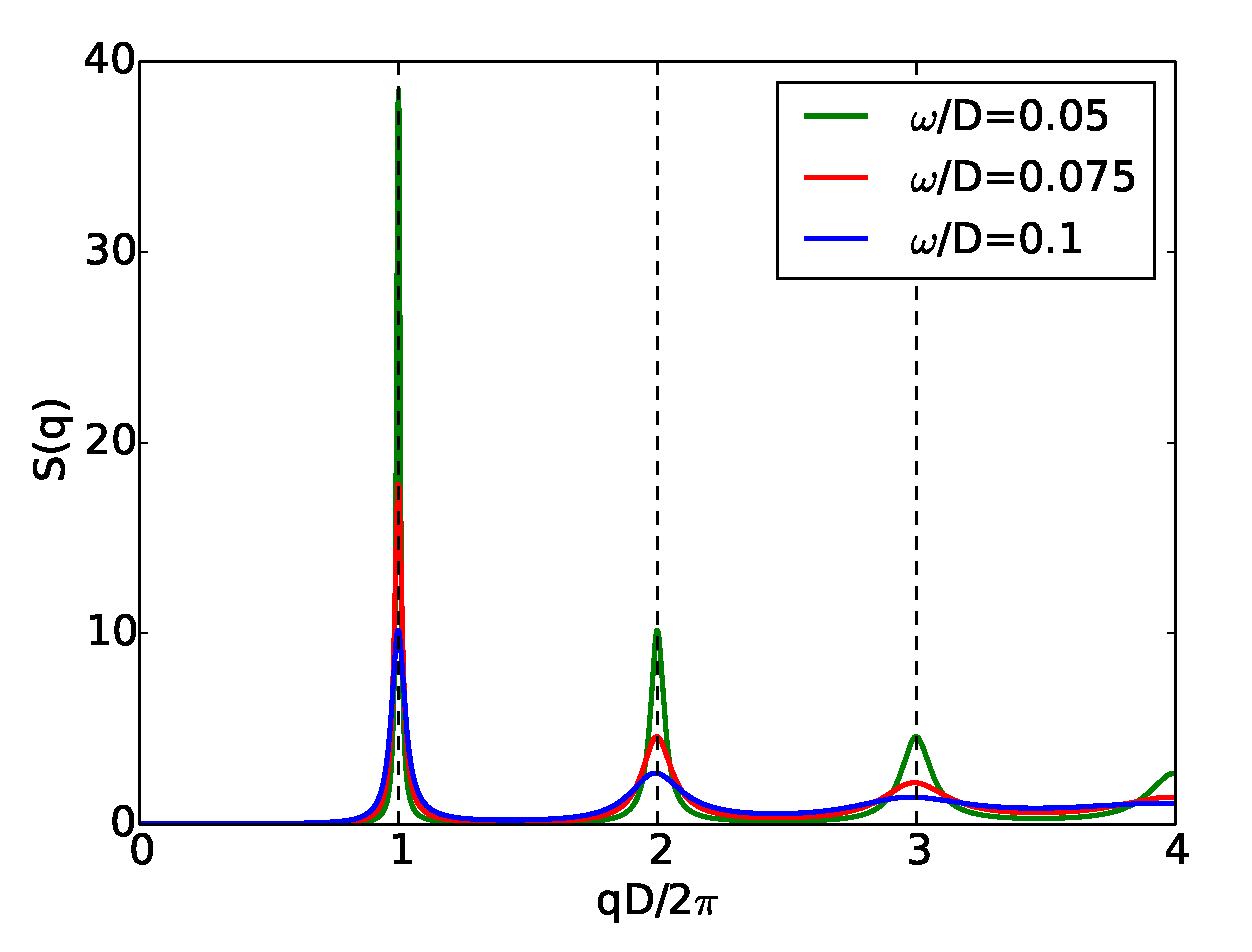
\includegraphics[width=0.6\textwidth]{fig/funcplot/S_q_1Dparacrystal.eps}
\end{center}
\caption{Interference function of a 1D Gaussian paracrystal plotted for different values of $\omega /D$. The peaks broaden with a decreasing amplitude as $\omega/D$ increases. This shows the transition between an ordered and a disordered states. }
\label{fig:1dparas_q}
\end{figure}

In two dimensions, the paracrystal is constructed on a pseudo-regular lattice with base vectors $\v{a}$ and $\v{b}$ using the following conditions for the densities of probabilities:\\ $\int p_{\v{a}}(\r)d^2r=\int p_{\v{b}}(\r)d^2r=1$, $\int \r p_{\v{a}}(\r)d^2r=\v{a}$, $\int \r p_{\v{b}}(\r)d^2r=\v{b}$.\\
In the ideal case the deformations along the two axes are decoupled and each unit cell should retain a parallelogram shape. The interference function is given by\\ $S(q_{\plll})=\prod_{k=a,b}\Re\left(\dfrac{1+P_k(q_{\plll})}{1-P_k(q_{\plll})} \right)$ with $P_k$ the Fourier transform of $p_k$, $k=a, b$.

\paragraph{Probability distributions} \mbox{}\\
The scattering by an ordered lattice gives rise to a series of Bragg peaks situated at the nodes of the reciprocal lattice. Any divergence from the ideal crystalline case modifies the output spectrum by, for example, widening or attenuating the Bragg peaks. The influence of these "defects" can be accounted for
 in direct space by using correlation functions or by truncating the lattice or, in reciprocal space with structure factors or interference functions by convoluting the scattered peaks with a function which could reproduce the experimental shapes.

%===============================================================================
\subsection{Size-Spacing Correlation Approximation}
%===============================================================================
\index{Size-spacing correlation approximation}

TO MERGE IN:
introduces correlations between polydisperse particles, more precisely between the size of the particles and their mutual spacing. A classical example would consist in particles whose closest-neighbor spacing depends linearly on the sum of their respective sizes \cite{LaLR07}, as illustrated in fig.~\ref{fig:ssca}.

%For a sample where only the statistical properties of particle positions and size are known, the scattered intensity per scattering particle is expressed as the average over an ensemble of the Fourier transform of the Patterson function, which is the autocorrelation of the scattering length density $\curlp (\r ) \equiv \sum_{ij} S_i(-\r )\otimes S_j(\r )\otimes \delta (\r + \r_i - \r_j )$:
%\begin{equation*}
%  I(\q ) = \frac{1}{N}\ensavg{}{\curlf (\curlp (\r ))},
%\end{equation*}
%where $\curlf$ denotes the Fourier transform and $\curlp$ the Patterson function

\begin{figure}[tb]
\begin{center}
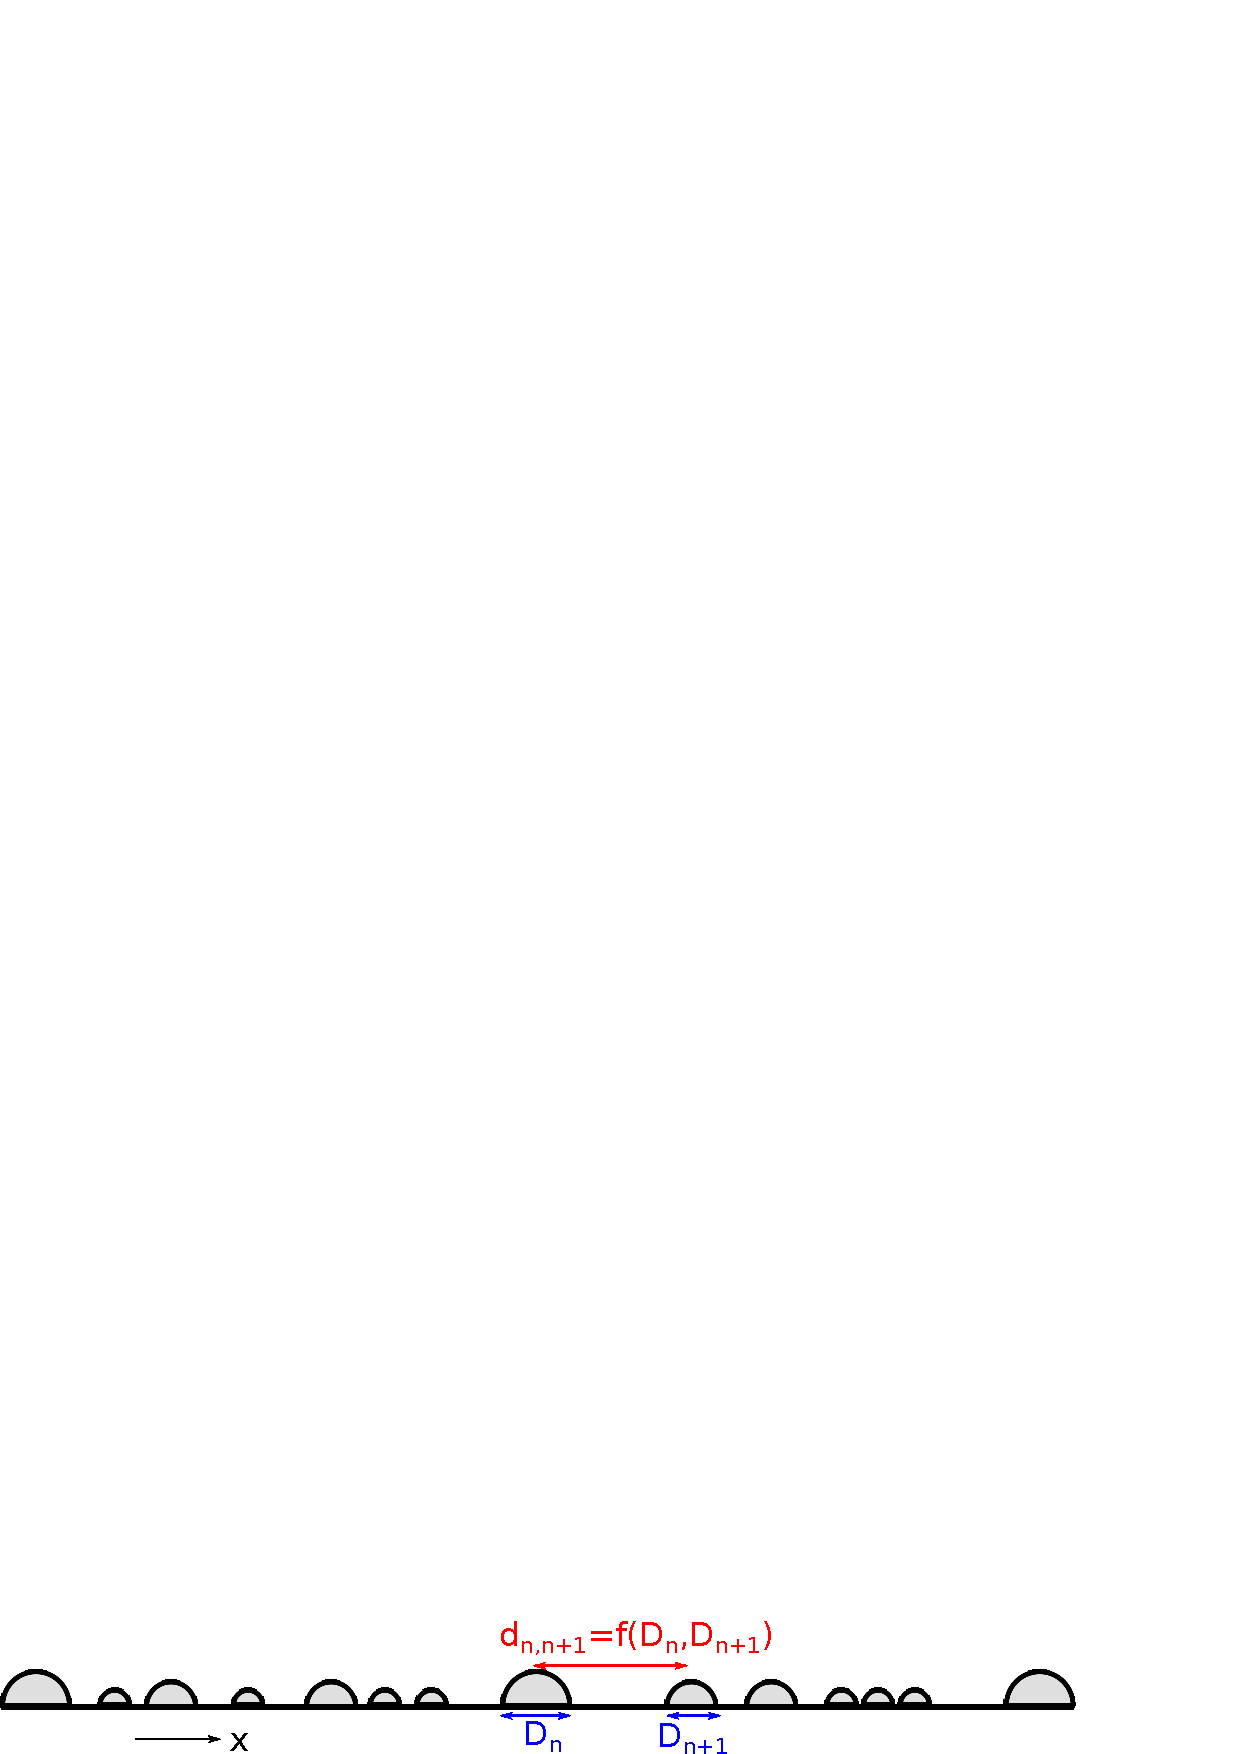
\includegraphics[width=0.9\textwidth]{fig/drawing/drawingSSCA.pdf}
\end{center}
\caption{Sketch of a 1D distributed collection of particles, whose scattering could be described by the size-spacing correlation approximation: the distance between two particles depends on their sizes.}
\label{fig:ssca}
\end{figure}


In the Size-Spacing Correlation Approximation, a correlation is assumed between the shape/size of the particles and their mutual spacing. A classical example would consist of particles whose closest-neighbor spacing depends linearly on the sum of their respective sizes. The following discussion of this type of correlation is inspired by \cite{LaLR07}

The scattered intensity can also be calculated as the Fourier transform of the Patterson function, which is the autocorrelation of the scattering length density:
\begin{equation*}
  \curlp (\r ) \equiv \sum_{ij} S_i(-\r )\otimes S_j(\r )\otimes \delta (\r + \r_i - \r_j ).
\end{equation*}
For a sample where only the statistical properties of particle positions and shape/size are known, the scattered intensity per scattering particle becomes average over an ensemble of the Fourier transform of the Patterson function:
\begin{equation*}
  I(\q ) = \frac{1}{N}\bra\curlf (\curlp (\r ))\ket,
\end{equation*}
where $\curlf$ denotes the Fourier transform.

The ensemble averaged Patterson function will be denoted as:
\begin{equation*}
  Z(r) \equiv \frac{1}{N}\bra\curlp (\r )\ket.
\end{equation*}
In the case of systems where the particles are aligned in one dimension, this autocorrelation function can be further split into nearest neighbor probabilities. First, it is split into terms for negative, zero or positive distance:
\begin{equation*}
  Z(\r ) \equiv z_0(\r ) + z_+(\r ) + z_-(\r ).
\end{equation*}
Taking $x$ as the coordinate in the direction in which the particles are arranged and $s$ as an orthogonal coordinate ($\r \equiv (x,s)$), one obtains:
\begin{align*}
  z_0(\r ) &= \sum_{\alpha_0} p(\alpha_0) S_{\alpha_0}(-x,-s) \otimes S_{\alpha_0}(x,s)  \\
  z_+(\r ) &= \sum_{\alpha_0\alpha_1} p(\alpha_0,\alpha_1) S_{\alpha_0}(-x,-s) \otimes S_{\alpha_1}(x,s) \otimes P_1(x|\alpha_0\alpha_1)  \\
               &+ \sum_{\alpha_0\alpha_1\alpha_2} p(\alpha_0,\alpha_1,\alpha_2) S_{\alpha_0}(-x,-s) \otimes S_{\alpha_2}(x,s) \otimes P_1(x|\alpha_0\alpha_1) \otimes P_2(x|\alpha_0\alpha_1\alpha_2)  \\
               &+ \dotsb \\
  z_-(\r ) &= z_+(-\r ),
\end{align*}
where $p(\alpha_0,\dotsc ,\alpha_n)$ denotes the probability of having a sequence of particles of the indicated sizes/shapes and $P_n(x|\alpha_0\dotsc\alpha_n)$ is the probability density of having a particle of type $\alpha_n$ at a (positive) distance $x$ of its nearest neighbor of type $\alpha_{n-1}$ in a sequence of the given order.

In the Size-Spacing Correlation Approximation, one assumes that the particle sequence probabilities are just a product of their individual fractions:
\begin{equation*}
  p(\alpha_0,\dotsc ,\alpha_n) = \prod_i p(\alpha_i),
\end{equation*}
and the nearest neighbor distance distribution is dependent only on the two particles involved:
\begin{equation*}
  P_n(x|\alpha_0\dotsc\alpha_n) = P_1(x|\alpha_{n-1}\alpha_n).
\end{equation*}
Furthermore, the distance distribution $P_1(x|\alpha_0\alpha_1)$ depends on the particle sizes/shapes only through its mean value $D$:
\begin{equation*}
  P_1(x|\alpha_0\alpha_1) = P_0(x - D(\alpha_0,\alpha_1) ),
\end{equation*}
where $D(\alpha_0,\alpha_1) = D_0 + \kappa \left[ \Delta R(\alpha_0) + \Delta R(\alpha_1) \right]$, with $\Delta R(\alpha_i)$ the deviation of a size parameter of particle $i$ with respect to the mean over all particles sizes/shapes and $\kappa$ the coupling parameter.

In momentum space, the sum of convolutions can be written as a geometric series, which can be exactly calculated to be:
\begin{equation}
\label{Esscainf}
I(\q ) = {\bra\left| F_\alpha(\q ) \right| ^2\ket}_{\alpha}
+ 2 \Re \left\lbrace \widetilde{\curlf_\kappa}(\q )
 \widetilde{\curlf_\kappa^*}(\q ) \cdot
 \frac{\Omega_\kappa(\q )}{\tilde{p}_{2\kappa}(\q )\left
   [ 1 - \Omega_\kappa(\q )\right] } \right\rbrace,
\end{equation}
with
\begin{align*}
  \tilde{p}_\kappa(\q ) &= \int d\alpha\; p(\alpha) e^{i\kappa q_x \Delta R(\alpha)}  \\
  \Omega_\kappa(\q ) &= \tilde{p}_{2\kappa}(\q ) \phi(\q) e^{i q_x D_0}  \\
  \widetilde{\curlf_\kappa}(\q ) &= \int d\alpha\; p(\alpha)F_\alpha (\q ) e^{i\kappa q_x \Delta R(\alpha)},
\end{align*}
and the Fourier transform of $P_1(x|\alpha_0\alpha_1)$ is
\begin{equation*}
  \curlp (\q ) = \phi (\q )e^{i q_x D_0} e^{i \kappa q_x \left[ \Delta R(\alpha_0) + \Delta R(\alpha_1) \right] }.
\end{equation*}

Using the result from the one-dimensional analysis, one can apply this formula ad hoc for distributions of particles in a plane, where the coordinate $x$ will now be replaced with $(x,y)$, while the $s$ coordinate encodes a position in the remaining orthogonal direction. One must be aware however that this constitutes a further approximation, since this type of correlation does not have a general solution in more than one dimension.

The intensity in (\ref{Esscainf}) will contain a Dirac delta function contribution, caused by taking an infinite sum of terms that are perfectly correlated at $\q = 0$. One can leverage this behaviour by multiplying the nearest neighbor distribution by a constant factor $e^{-D/\Lambda}$, which removes the division by zero in (\ref{Esscainf}).
Another way of dealing with this infinity at $\q =0$ consists of taking only a finite number of terms, in which case the geometric series still has an analytic solution, but becomes a bit more cumbersome:
\begin{equation*}
\begin{split}
  I(\q ) &= {\bra\left| F_\alpha(\q ) \right| ^2\ket}_\alpha
   + 2 \Re \Biggl\lbrace \frac{1}{\tilde{p}_{2\kappa}(\q )}\widetilde{\curlf_\kappa}(\q )\widetilde{\curlf_\kappa^*}(\q ) \\
  & \times \left[ \left( 1 - \frac{1}{N}\right) \frac{\Omega_\kappa(\q )}{1 - \Omega_\kappa(\q ) } - \frac{1}{N}\frac{\Omega_\kappa^2(\q )\left( 1- \Omega_\kappa^{N-1}(\q )\right) }{\left( 1 - \Omega_\kappa(\q ) \right) ^2 } \right] \Biggr\rbrace.
\end{split}
\end{equation*}
This expression has a well-defined limit for $\Omega_\kappa(\q ) \rightarrow 1$ (when $\q \rightarrow 0$), namely:
\begin{equation*}
  \lim_{\q \rightarrow 0} I(\q ) = {\bra\left| F_\alpha(0 ) \right| ^2\ket}_{\alpha} + \left( N-1 \right) \left| {\bra F_\alpha(0 )\ket}_{\alpha} \right|^2.
\end{equation*}


%%%%%%%%%%%%%%%%%%%%%%%%%%%%%%%%%%%%%%%%%%%%%%%%%%%%%%%%%%%%%%%%%%%%%%%%%%%%%%%%
\section{Vertical location of particles}
%%%%%%%%%%%%%%%%%%%%%%%%%%%%%%%%%%%%%%%%%%%%%%%%%%%%%%%%%%%%%%%%%%%%%%%%%%%%%%%%

 \ImportantPoint{Remark:}{The particles cannot sit in between layers. At most they can be sitting on any inner interfaces.}

%===============================================================================
\subsection{Particles deposited on a substrate}
%===============================================================================
%Substrate modified Born approximation
In this configuration, the particles are sitting on top of a substrate layer, in the air as shown in fig.~\ref{fig:SchemDWBA}. In the DWBA the expression of a form factor becomes
\begin{align}
F_{\rm{DWBA}}(q_{\plll}, k_{i,z}, k_{f,z}) &= F_{\rm{BA}}(q_{\plll}, k_{i,z}-k_{f,z})+ R_i F_{\rm{BA}}(q_{\plll}, -k_{i,z}-k_{f,z}) \nonumber \\
&+ R_f F_{\rm{BA}}(q_{\plll}, k_{i,z}+k_{f,z}) + R_i R_f F_{\rm{BA}}(q_{\plll},-k_{i,z}+k_{f,z}), \label{Edwbaair}
\end{align}
where $q_{\plll}$ is the component of the scattering beam in the plane of the interface ($\q=\k_i-\k_\text{f}$), $k_{i,z}$ and $k_{f,z}$ are the z-component of the incident and scattered beam, respectively. $R_i$, $R_f$ are the reflection coefficients in incidence and reflection. They are defined as\\ $R=\dfrac{k_z+\sqrt{n_s^2k_0^2-|k_{\plll}|^2}}{k_z-\sqrt{n_s^2 k_0^2-|k_{\plll}|^2}}$, where $n_s=1-\delta_s +i \beta_s$ is the refractive index of the substrate, $k_0$ is the wavelength in vacuum ($2\pi /\lambda$), $k_z$ and $k_{\plll}$ are the $z$-component and the in-plane component of $\k_\text{i}$ or $\k_\text{f}$. \\

\ImportantPoint{Remark:}{If the particles are sitting on a multilayered system, the expression of the form factor in the DWBA is obtained by replacing the Fresnel coefficient by the corresponding coefficients of the underlying layers \cite{Par54,BoWo99}.}

\vspace{18pt}

Figure~\ref{fig:SchemDWBA} illustrates the four scattering processes for a supported particle, taken into account in the DWBA. The first term of eq.~\ref{Edwbaair}  corresponds to the Born approximation. Each term of $F_{\rm{DWBA}}$ is weighted by a Fresnel coefficient.

\begin{figure}[tb]
\begin{center}
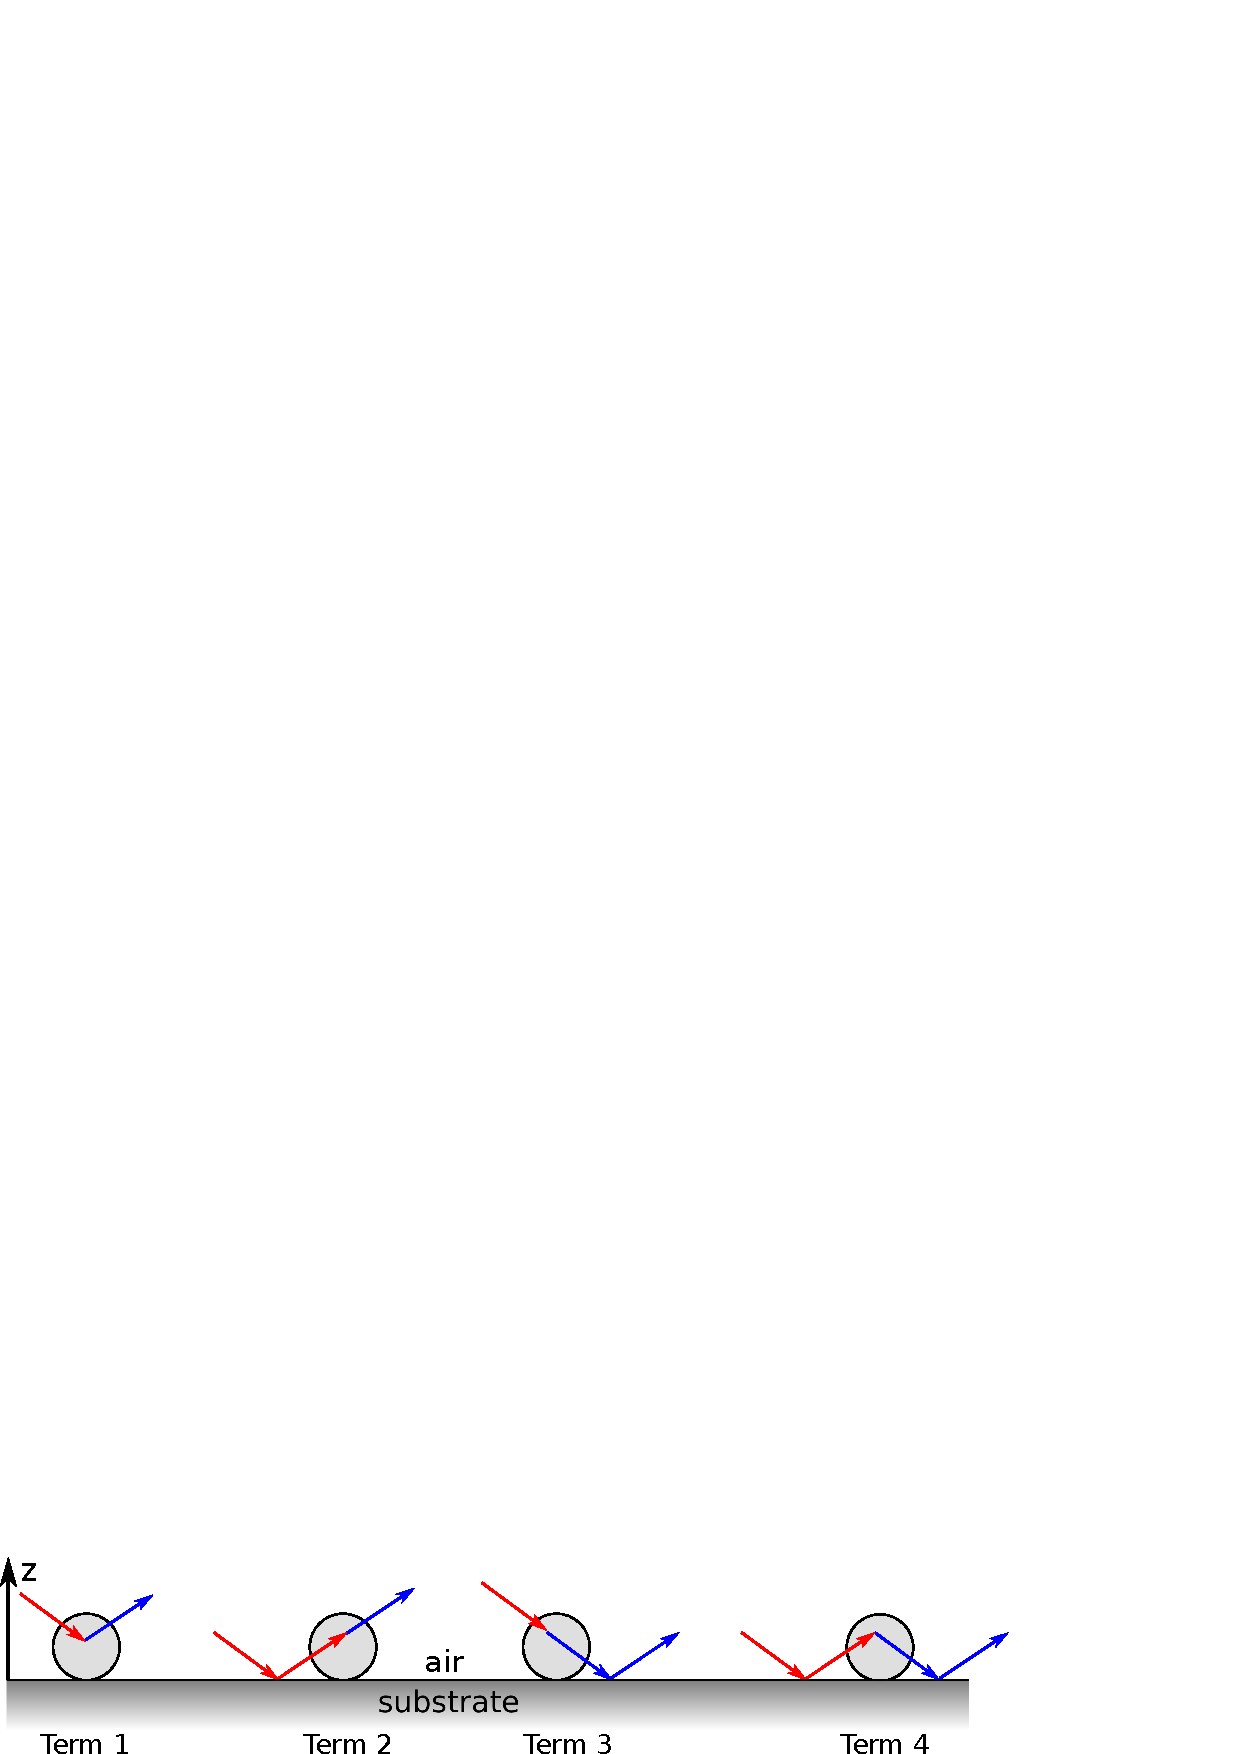
\includegraphics[width=\textwidth]{fig/drawing/drawingDWBA.pdf}
\end{center}
\caption{Schematic views of the different terms appearing in the expression of the form factor under DWBA for particles sitting on a substrate layer.}
\label{fig:SchemDWBA}
\end{figure}


Script~\ref{lst:badwba} illustrates the difference between BA and DWBA in \BornAgain\ when generating the sample.  We consider the simple case of:
\begin{itemize}
\item one kind of particles' shape,
\item no interference between the particles,
\item in the DWBA, a sample made of a layer of substrate on which are deposited the particles,
\item in the BA, a sample composed of the particles in air.
\end{itemize}

Figure~\ref{fig:spheroidbadwba} shows the intensity contour plot generated using this script with truncated spheroids as particles.

\newpage

\begin{lstlisting}[language=python, style=eclipseboxed,numbers=none,nolol,caption={\Code{Python} script to generate a sample using Born (BA) or distorted-wave Born approximation (DWBA). The difference between BA and DWBA in this simple case is the absence or presence of a substrate layer in the sample.},label={lst:badwba}]
def get_sample():
    """
    Build and return the sample to calculate form factor of
    truncated spheroid in Born or distorted-wave Born Approximation.
    """
    # defining materials
    m_ambience = HomogeneousMaterial("Air", 0.0, 0.0)
    m_substrate = HomogeneousMaterial("Substrate", 6e-6, 2e-8)
    m_particle = HomogeneousMaterial("Particle", 6e-4, 2e-8)

    # collection of particles
    ff= FormFactorTruncatedSpheroid(7.5*nanometer, 9.0*nanometer, 1.2)
    particleshape = Particle(m_particle, ff)
    particle_layout = ParticleLayout()
    particle_layout.addParticle(particleshape, 1.0)

    # interferences
    interference = InterferenceFunctionNone()
    particle_layout.addInterferenceFunction(interference)

    # assembling the sample
    air_layer = Layer(m_ambience)
    air_layer.addLayout(particle_layout)
    substrate_layer = Layer(m_substrate, 0)

    multi_layer = MultiLayer()
    multi_layer.addLayer(air_layer)
    # Comment the following line out for Born Approximation
    multi_layer.addLayer(substrate_layer)
    return multi_layer
\end{lstlisting}


\begin{figure}[tb]
\hfill
\subfigure[Born Approximation]{\includegraphics[angle=-90,width=6cm]{fig/gisasmap/ffspheroidBA.pdf}}
\hfill
\subfigure[DWB Approximation]{\includegraphics[angle=-90,width=6cm]{fig/gisasmap/ffspheroidDWBA.pdf}}
\hfill
\caption{Intensity map of TruncatedSpheroid form factor in BA and DWBA computing using script~\ref{lst:badwba} for the sample.}
\label{fig:spheroidbadwba}
\end{figure}

\FloatBarrier

\ImportantPoint{Remark:}{In \BornAgain, the DWBA is implemented automatically when assembling the sample with more layers than only the air layer (for example, for particles are sitting on a substrate).}

%===============================================================================
\subsection{Buried particles}
%===============================================================================

The system considered in this section consists of particles encapsulated in a layer, which is sitting on a substrate (see fig.~\ref{fig:SchemDWBAburied}). In this case the form factor in the DWBA is given by

\begin{align}
  F_{\rm{DWBA}}(q_{\plll}, k_{i,z}, k_{f,z})
  &= T_\text{i} T_\text{f} F_{\rm{BA}}(q_{\plll}, k_{i,z}-k_{f,z})e^{i(k_{i,z}-k_{f,z})d}\nonumber \\
  &+ R_\text{i} T_\text{f} F_{\rm{BA}}(q_{\plll}, -k_{i,z}-k_{f,z})e^{i(-k_{i,z}-k_{f,z})d} \nonumber \\
  &+ R_\text{f} T_\text{i} F_{\rm{BA}}(q_{\plll}, k_{i,z}+k_{f,z}) e^{i(k_{i,z}+k_{f,z})d}\nonumber \\
  &+ R_\text{f} R_\text{i}F_{\rm{BA}}(q_{\plll},-k_{i,z}+k_{f,z})e^{i(-k_{i,z}+k_{f,z})d}, \label{Edwbaburied}
\end{align}

\begin{equation*}
R_j =\frac{t^{j}_{0,1}r^{j}_{1,2}\exp(2ik_{j,z}t)}{1+r^{j}_{0,1}r^{j}_{1,2}\exp(2ik_{j,z}t)}, \quad T_j=\frac{t^{j}_{0,1}}{1+r^{j}_{0,1}r^{j}_{1,2}\exp(2ik_{j,z}t)}, j=i,f
\end{equation*}
where $q_{\plll}$ is the component of the scattering beam in the plane of the interface, $k_{i,z}$ and $k_{f,z}$ are the z-component of the incident and scattered beams, respectively.  $d$ is the depth at which the particles are sitting in the layer. Note that this value is given relative to the top of this layer and it is not the coordinate in the absolute referential (linked with the full sample) and it is measured up to the bottom of the particle. $t$ is the thickness of the intermediate layer containing the particles. $R_{i,f}$ and $T_{i,f}$  are the reflection  and transmission coefficients in incidence and reflection (they can be calculated using Parratt or matrix formalism). $r^j_{0,1}$, $r^j_{1,2}$ $t^j_{0,1}$ are the reflection and transmission coefficients between layers; the indices are related to different boundaries with 0: air, 1: intermediate layer and 2: substrate layer and the superscript $j$ is associated with the incident or scattered beams:
\begin{equation*}
r^j_{n,n+1}=\frac{k_{j,z,n}-k_{j,z,n+1}}{k_{j,z,n}-k_{j,z,n+1}}, \qquad t^j_{n,n+1}= \frac{2k_{j,z,n}}{k_{j,z,n}-k_{j,z,n+1}}, \quad n=0,1, \quad j=i,f,
\end{equation*}
where index $n$ is related to the layers, $z$ to the vertical component, and $j$ to the beams (incident and outgoing).

\begin{figure}[tb]
\begin{center}
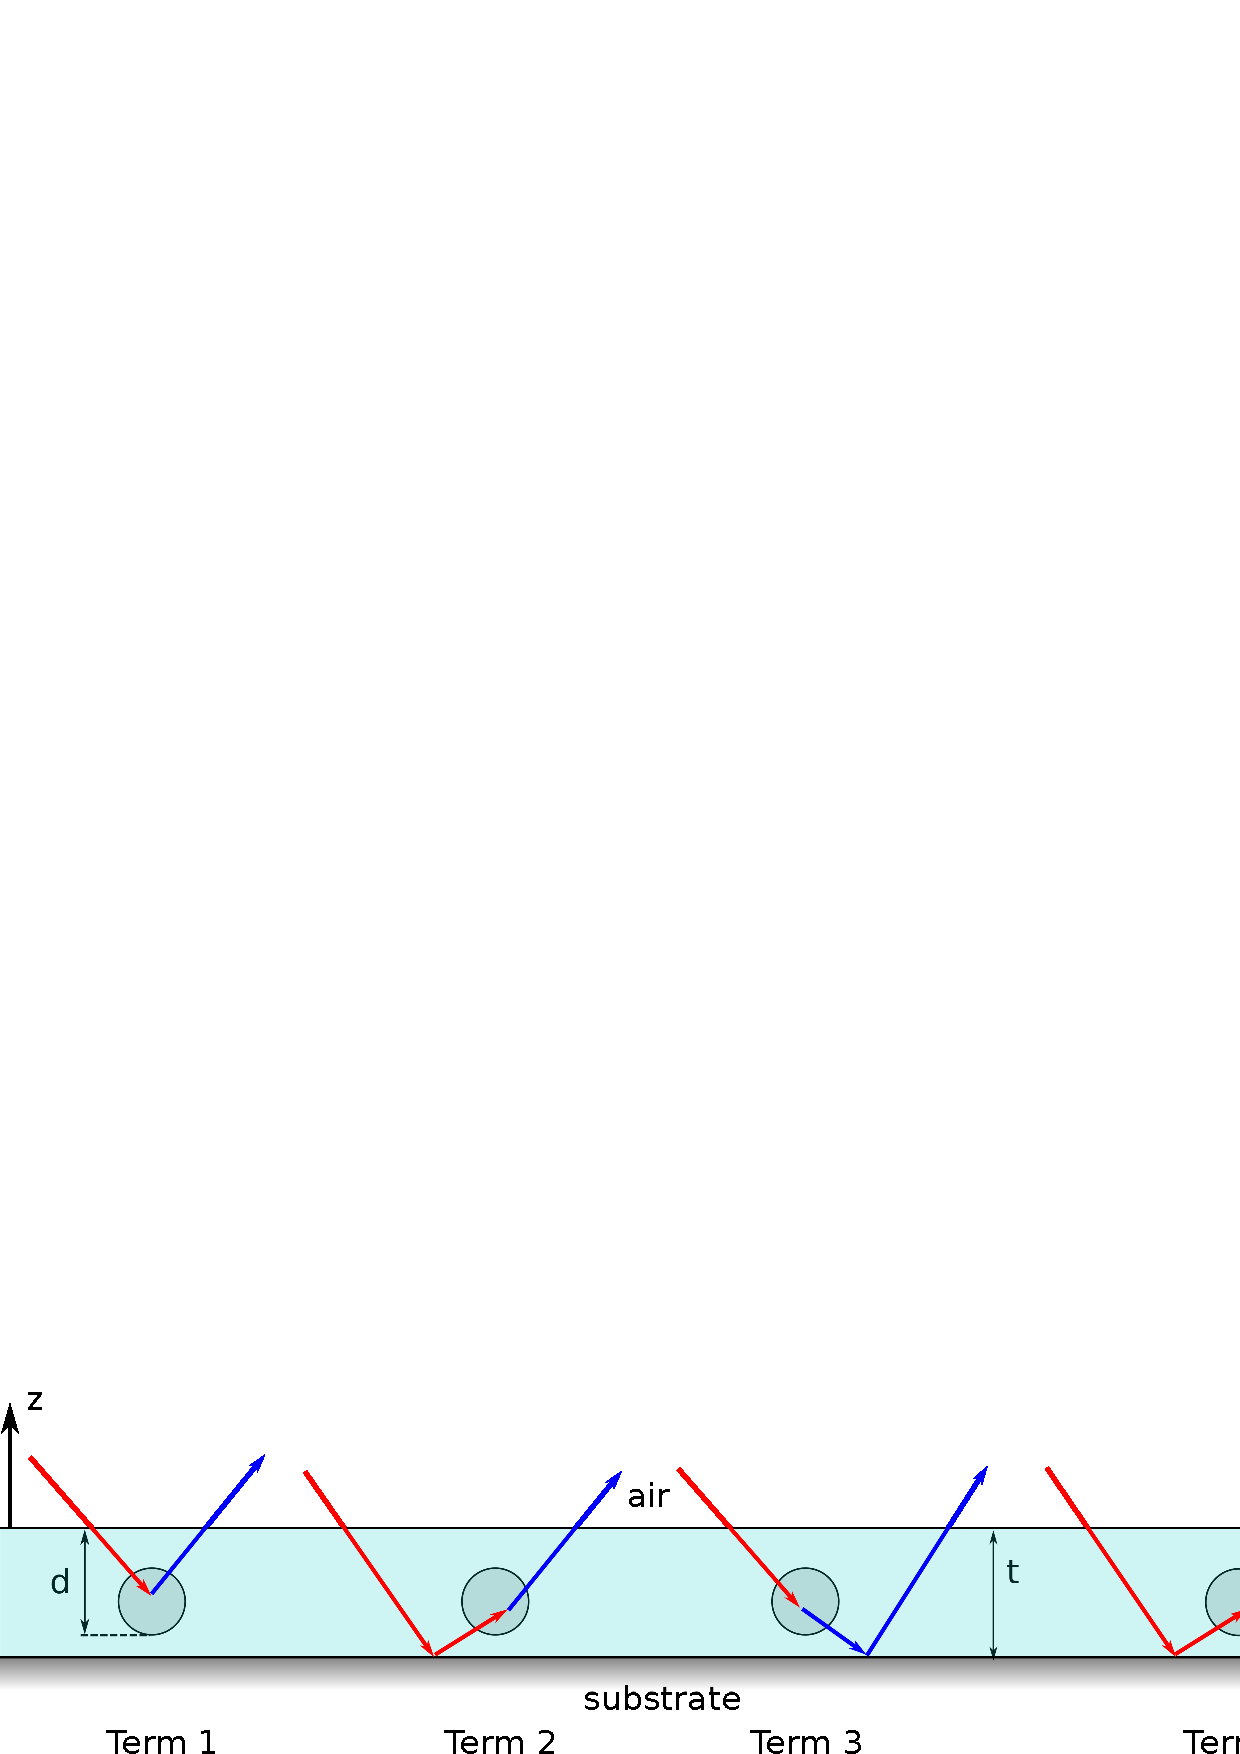
\includegraphics[width=\textwidth]{fig/drawing/drawingDWBAburied.pdf}
\end{center}
\caption{Schematic views of the different terms appearing in the expression of the form factor under the DWBA for buried particles.}
\label{fig:SchemDWBAburied}
\end{figure}


Figure~\ref{fig:dwbaburied} shows a typical example of the output intensity scattered from a sample made of 3 layers: air, substrate, and in between, spherical particles embedded in the middle of a 30~nm-thick layer. This figure had been generated using listing~\ref{lst:dwbaburied}.

\begin{lstlisting}[language=python, style=eclipseboxed,numbers=none,nolol,caption={\Code{Python} script to generate a sample where spherical particles are embedded in the middle of a layer on a substrate.},label={lst:dwbaburied}]
def get_sample():
    """
    Build and return the sample with buried spheres in DWBA.
    """
    # defining materials
    m_ambience = HomogeneousMaterial("Air", 0.0, 0.0)
    m_interm_layer = HomogeneousMaterial("IntermLayer",3.45e-6, 5.24e-9)
    m_substrate = HomogeneousMaterial("Substrate", 7.43e-6, 1.72e-7)
    m_particle = HomogeneousMaterial("Particle", 0.0, 0.0)

    # collection of particles
    ff = FormFactorFullSphere(10.2*nanometer)
    particleshape = Particle(m_particle, ff)
    particleshape.setPosition(0.0, 0.0, -25.2)
    particle_layout = ParticleLayout()
    particle_layout.addParticle(particleshape, 1.0)

    # interferences
    interference = InterferenceFunctionNone()
    particle_layout.addInterferenceFunction(interference)

    # assembling the sample
    air_layer = Layer(m_ambience)
    intermediate_layer = Layer(m_interm_layer, 30.*nanometer)
    intermediate_layer.addLayout(particle_layout)
    substrate_layer = Layer(m_substrate, 0)

    multi_layer = MultiLayer()
    multi_layer.addLayer(air_layer)
    multi_layer.addLayer(intermediate_layer)
    multi_layer.addLayer(substrate_layer)
    return multi_layer
\end{lstlisting}


\begin{figure}[tb]
\centering
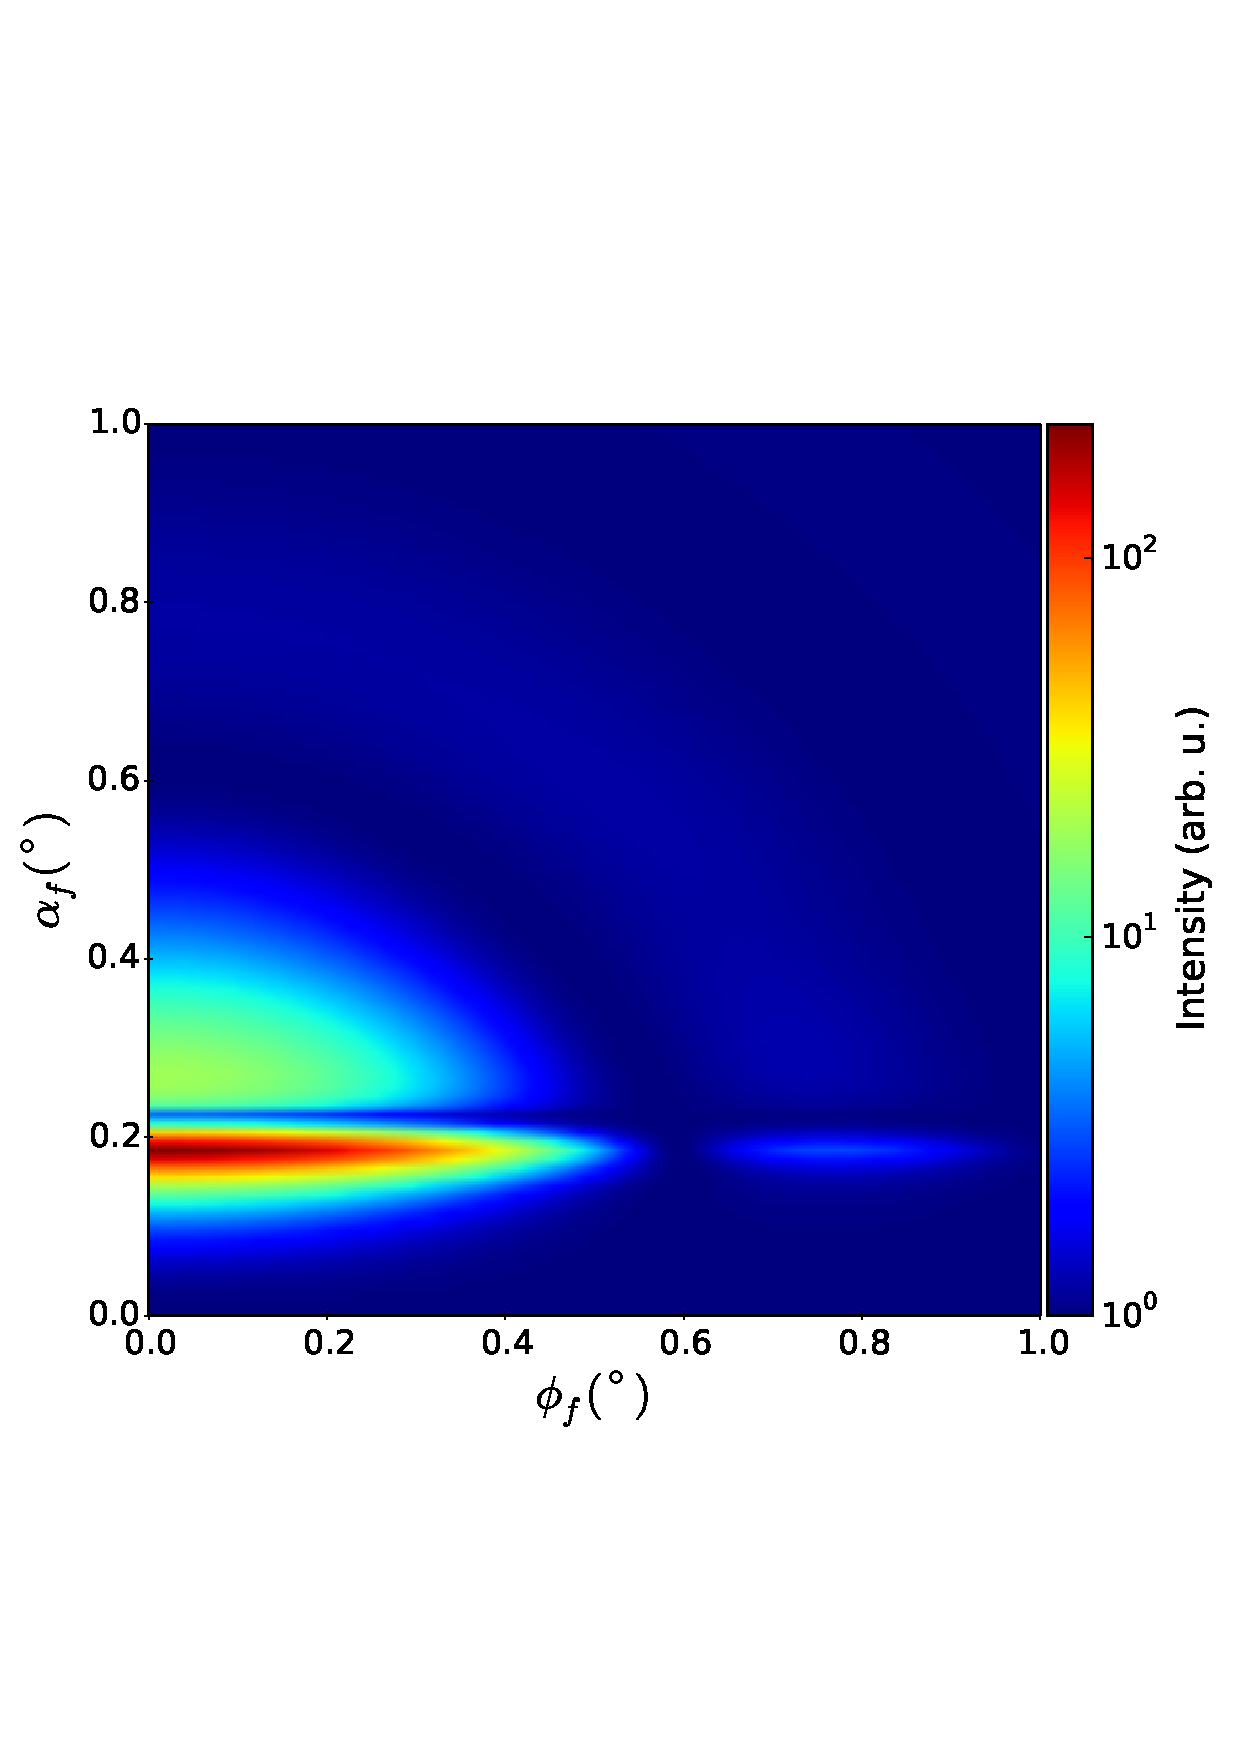
\includegraphics[angle=-90,width=0.6\textwidth]{fig/gisasmap/figIntBuriedPart.pdf}
\caption{Map of intensity scattered from a sample made of spherical particles embedded in the middle of a 30~nm-thick layer on a substrate (see Script~\ref{lst:dwbaburied} for details about the sample).}
\label{fig:dwbaburied}
\end{figure}

\newpage

\ImportantPoint{Remark:}{For layers different from the air layer, the top interface is considered as the reference level to position the encapsulated particles. For example, spheres positioned at depth $d$ (positive) are located at a distance $d$ from the top of the layer up to the bottom of these particles. This convention is different for the top air layer, where particles sitting at the interface with an underlying layer (\idest the bottom of the air layer) are located at depth 0 (see fig.~\ref{fig:depthpartBA}).}


\begin{figure}[tb]
\centering
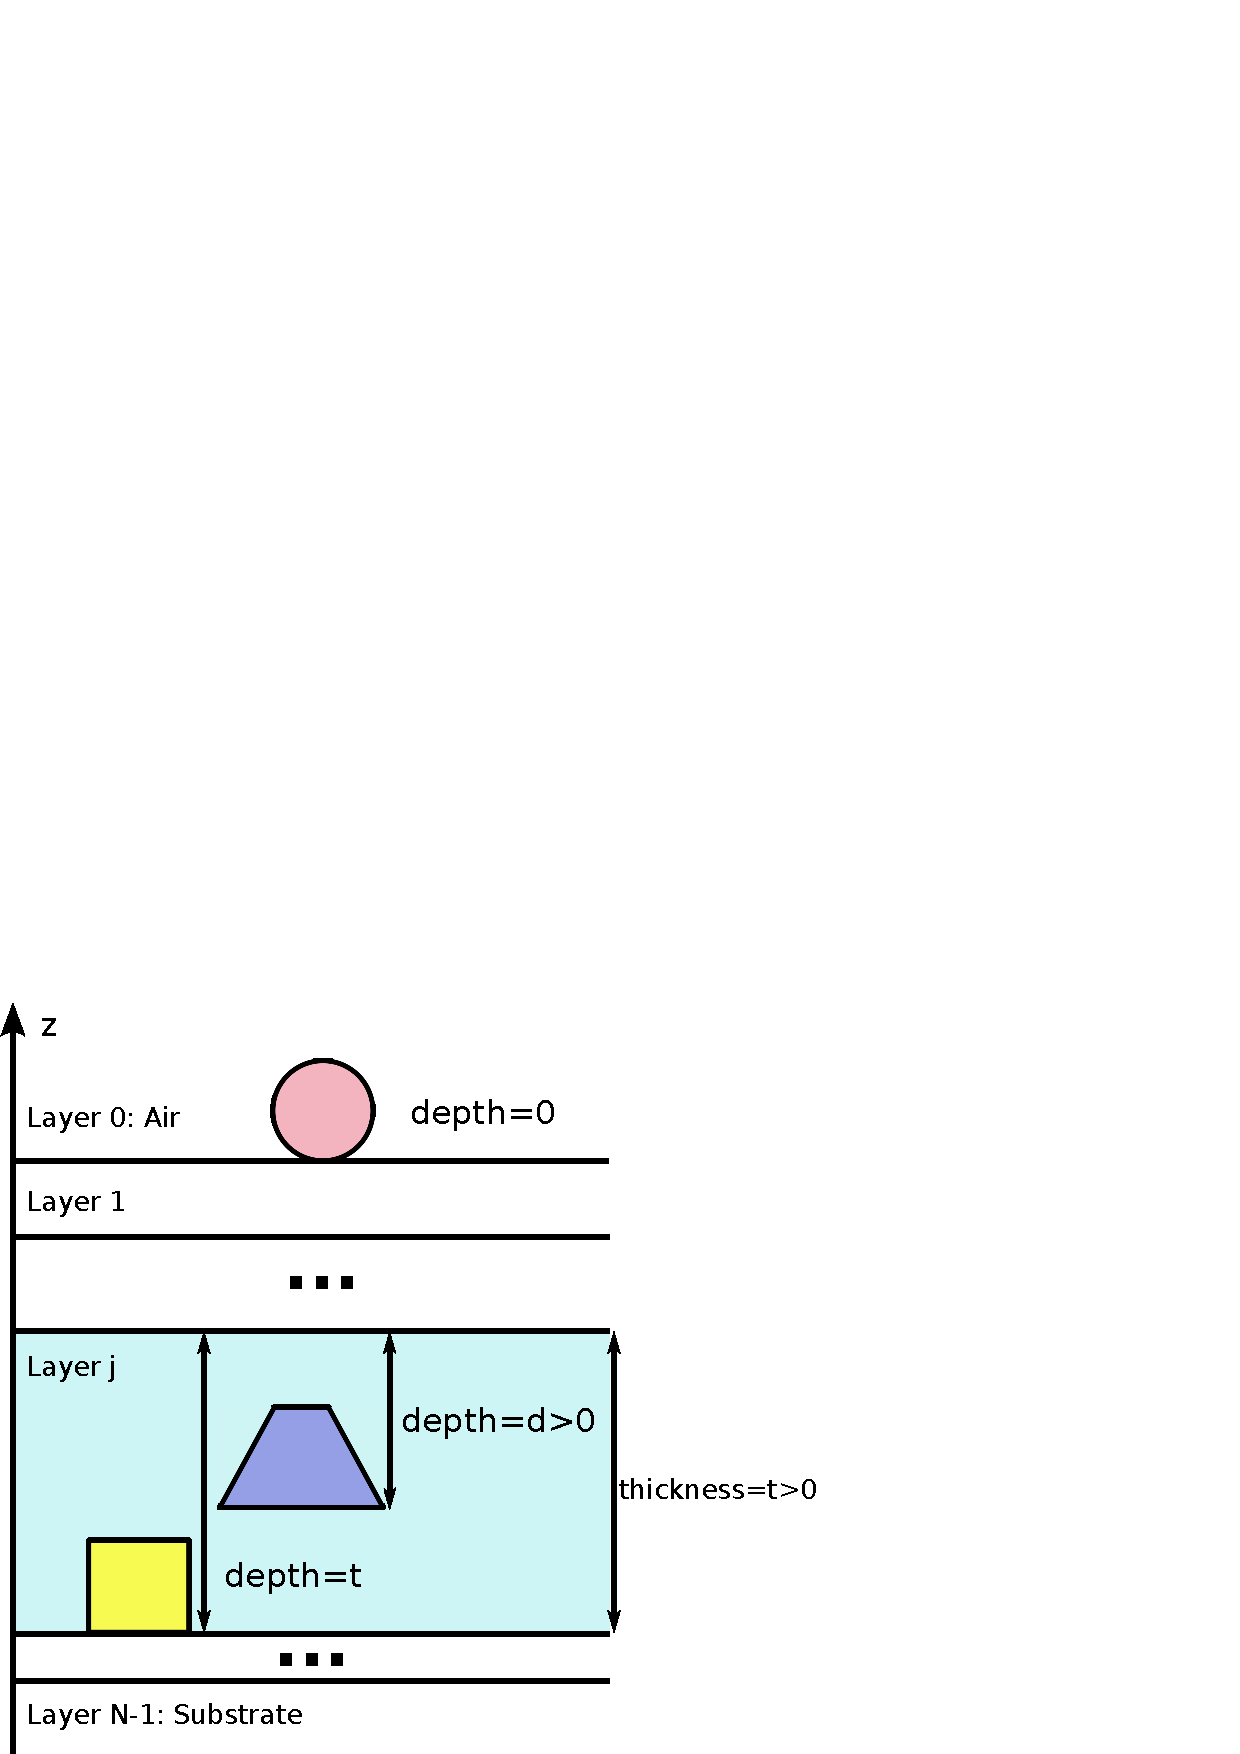
\includegraphics[width=0.5\textwidth]{fig/drawing/drawingDepthParticle.pdf}
\caption{Illustration of the convention about \Code{depth} used in \BornAgain\ to encapsulate particles in layers.}
\label{fig:depthpartBA}
\end{figure}


%%%%%%%%%%%%%%%%%%%%%%%%%%%%%%%%%%%%%%%%%%%%%%%%%%%%%%%%%%%%%%%%%%%%%%%%%%%%%%%%
\section{Implementation in \BornAgain}
%%%%%%%%%%%%%%%%%%%%%%%%%%%%%%%%%%%%%%%%%%%%%%%%%%%%%%%%%%%%%%%%%%%%%%%%%%%%%%%%

This section describes the implementation of the interference functions in \BornAgain.
For an implementation of all the components of a simulation,
the use is referred, for example, to Sec.~\ref{sec:Example1Python}.\\


\ImportantPoint{Remark:}{In \BornAgain\ the particles are positioned in the same vertical layer.}

\subsection{Size-distribution models}
\index{Size-distribution models}
The decoupling approximation (DA), local monodisperse approximation (LMA) and size spacing correlation approximation (SSCA) can be used in \BornAgain.
The selection between DA and SSCA is made using\\
\Code{ILayout.setApproximation(EInterferenceFunction approximation)} when defining the characteristics of the way particles and interference functions are embedded in a layer.  For example,
\begin{lstlisting}[language=python, style=eclipseboxed,numbers=none,nolol]
    particle_layout = ParticleLayout()
   ....
# interference approx chosen between: DA (default) and SSCA
    particle_layout.setApproximation(ILayout.DA)
\end{lstlisting}

Note that with the SSCA, the users have to specify the coupling parameter $\kappa$ (with the function \Code{setKappa}), which should be a positive dimensionless value. $\kappa$ characterizes the influence of the neighboring particles' sizes on their distance. If $\kappa=0$, the SSCA reduces to the DA with a radial paracrystal for the interference function.\\

For the LMA, its implementation is automatically done when using more than one layout of particles:
\begin{lstlisting}[language=python, style=eclipseboxed,numbers=none,nolol]
    particle_layout0 = ParticleLayout()
    particle_layout1 = ParticleLayout()
   ....
# association of each particles' layout with materials, form factors
#... and with a material layer
    layer_a = Layer(m_material_a)
    layer_a.addLayout(particle_layout0)
    layer_a.addLayout(particle_layout1)
\end{lstlisting}

%%ADD EXPLANATION ABOUT LMA

%-------------------------------------------------------------------------------
\subsection{Probability distribution functions}\label{baftd}
%-------------------------------------------------------------------------------

The probability distribution functions have been implemented in the reciprocal space in \BornAgain. Their expressions are given in Table~\ref{table:pdf}.

\begin{table}[H]
\centering
\begin{tabular}{ccc}
\hline
Function & One dimension & Two dimensions\\
\hline
Cauchy & $(1+q^2\omega^2)^{-3/2}$ & $(1 + q_x^2 cl_x^2 + q_y^2 cl_y^2)^{-3/2}$ \\
Gauss & $\dfrac{1}{2}\exp(-\dfrac{q^2\omega^2}{4})$ & $\frac{1}{2}\exp\left(-\dfrac{q_x^2 cl_x^2+ q_y^2cl_y^2}{4}\right)$ \\
Voigt & $\dfrac{\eta}{2} \exp\left(-\dfrac{q^2\omega^2}{4}\right) + \dfrac{1 - \eta}{(1 + q^2\omega^2)^{3/2}}$ & $\dfrac{\eta}{2} \exp\left(-\dfrac{q_x^2 cl_x^2+ q_y^2cl_y^2}{4}\right)+ \dfrac{1 - \eta}{(1 + q_x^2 cl_x^2+ q_y^2cl_y^2)^{3/2}}$ \\
\hline
\end{tabular}
\caption{List of probability distribution functions in reciprocal space. $\omega$, $cl$ stand for coherence lengths (the index refers to the axis) and  $\eta$ is a weighting coefficient.}
\label{table:pdf}
\end{table}

The Cauchy distribution corresponds to $\exp(-r)$ in real space and the Voigt one  is a linear combination of the Gaussian and Cauchy probability distribution functions.\\

\noindent \underline{One dimension}
\begin{itemize}
\item \Code{FTDistribution1DCauchy($\omega$)},
\item \Code{FTDistribution1DGauss($\omega$)},
\item \Code{FTDistribution1DVoigt($\omega, \eta$)}.
\end{itemize}
where $\omega$ is the coherence length and $\eta$ is a weighting factor.\\

\noindent \underline{Two dimensions}
\begin{itemize}
\item \Code{FTDistribution2DCauchy($cl_x$, $cl_y$)},
\item \Code{FTDistribution2DGauss($cl_x$, $cl_y$)},
\item \Code{FTDistribution2DVoigt($cl_x$, $cl_y$)}
\end{itemize}
where $cl_{x,y}$ are the coherence lengths in the $x$ or $y$ direction, respectively.

These functions can be used with all interference functions, except the case without any interference.

%-------------------------------------------------------------------------------
\subsection{Interferences}
%-------------------------------------------------------------------------------
\index{Interference function}

The interference function is specified when building the sample. It is linked with the particles (shape, material). Examples of implementation are given at the end of each description.

\paragraph{Syntax:}
 \Code{particle\_layout.addInterferenceFunction(interference\_function)},\\ where \Code{particle\_layout} holds the information about the different shapes and their proportions for a given layer of particles, and \Code{interference\_function}  is one of the following expressions:
\begin{itemize}
\item \Code{InterferenceFunctionNone()}
\item \Code{InterferenceFunction1DLattice(lattice\_parameters)}
\item \Code{InterferenceFunctionRadialParaCrystal(peak\_distance, damping\_length)}
\item \Code{InterferenceFunction2DLattice(lattice\_parameters)}
\item \Code{InterferenceFunction2DParaCrystal(length\_1, length\_2, $\alpha$\_lattice, $\xi$, \\ damping\_length)}
\end{itemize}

\ImportantPoint{Remark:}{\Code{InterferenceFunction1DLattice} can only be used for particles which are infinitely long in one direction of the sample's surface like for example a rectangular grating.}

\newpage
%-------------------------------------------------------------------------------
\subsection{InterferenceFunctionNone}
%-------------------------------------------------------------------------------

The particles are placed randomly in the dilute limit and are considered as individual, non-interacting scatterers. The scattered intensity is function of the form factors only.

\paragraph{Example} The sample is made of a substrate on which are deposited half-spheres. Script~\ref{lst:nointerf} details the commands necessary to generate such a sample. Figure~\ref{fig:nointerf} shows an example of output intensity: Script~\ref{lst:nointerf}  + detector's + input beam's characterizations.


\begin{figure}[tb]
\begin{center}
\includegraphics[angle=-90,width=0.5\textwidth]{fig/gisasmap/HSphere_NoInterf.pdf}
\end{center}
\caption{Output intensity scattered from a sample made of half-spheres with no interference between them.}
\label{fig:nointerf}
\end{figure}

\FloatBarrier
\newpage

\begin{lstlisting}[language=python, style=eclipseboxed,numbers=none,nolol,caption={\Code{Python} script to simulate a sample made of half-spheres deposited on a substrate layer without any interference. The part specific to the interferences is marked in a red italic font.},label={lst:nointerf}]
def get_sample():
    """
    Build and return the sample representing particles with no interference
    """
    # defining materials
    m_ambience = HomogeneousMaterial("Air", 0.0, 0.0)
    m_substrate = HomogeneousMaterial("Substrate", 6e-6, 2e-8)
    m_particle = HomogeneousMaterial("Particle", 6e-4, 2e-8)
    # collection of particles
    sphere_ff = FormFactorTruncatedSphere(5*nanometer, 5*nanometer)
    sphere = Particle(m_particle, sphere_ff)
    particle_layout = ParticleLayout()
    particle_layout.addParticle(sphere, 1.0)
    |interference = InterferenceFunctionNone()|
    |particle_layout.addInterferenceFunction(interference)|
    # assembling the sample
    air_layer = Layer(m_ambience)
    air_layer.addLayout(particle_layout)
    substrate_layer = Layer(m_substrate, 0)

    multi_layer = MultiLayer()
    multi_layer.addLayer(air_layer)
    multi_layer.addLayer(substrate_layer)
    return multi_layer
\end{lstlisting}

\newpage
%-------------------------------------------------------------------------------
\subsection{\Code{InterferenceFunction1DLattice(lattice\_length, xi)}}
%-------------------------------------------------------------------------------
where lattice\_length is the lattice constant and $\xi$ the angle in radian between the lattice unit vector and the $\v{x}$-axis of the reference Cartesian frame as shown in fig.~\ref{fig:1dgrating}.

\begin{figure}[tb]
\begin{center}
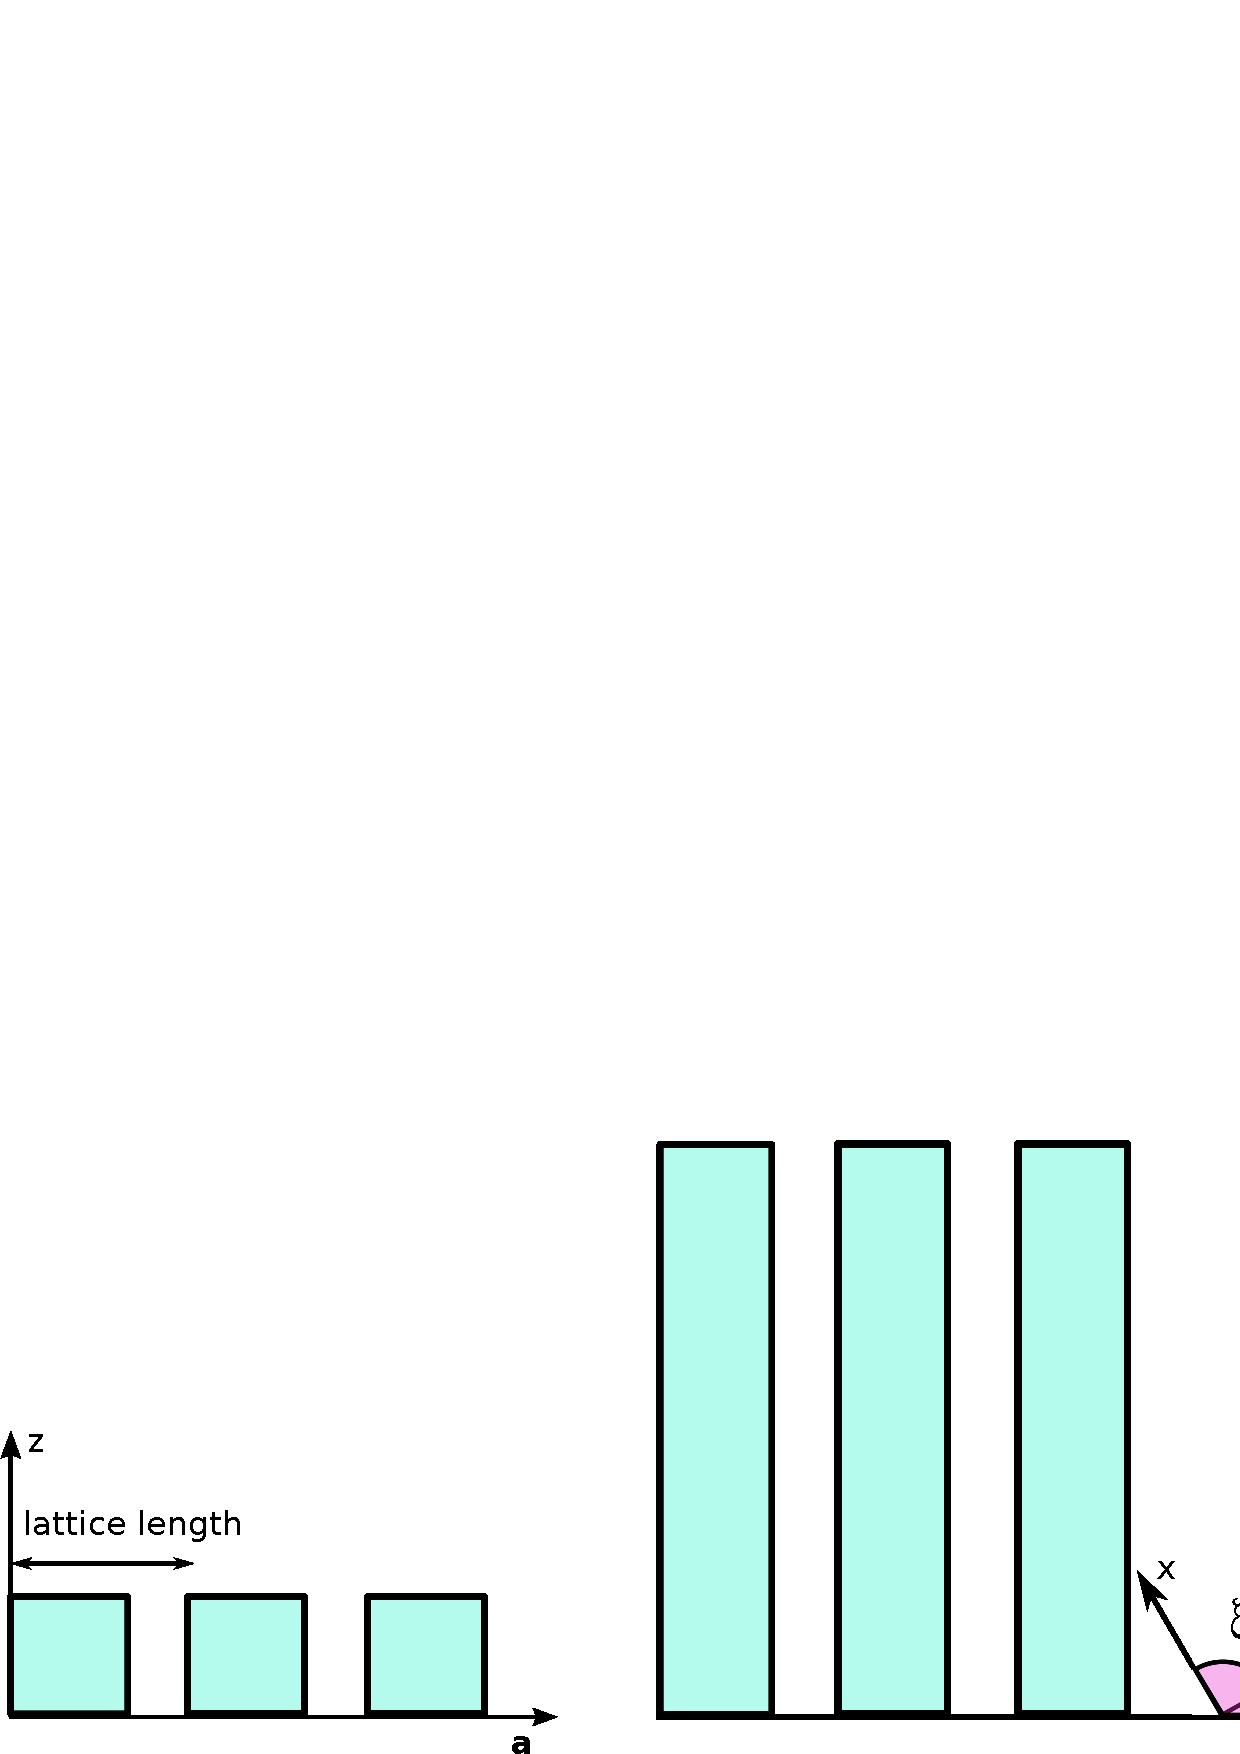
\includegraphics[width=0.75\textwidth]{fig/drawing/1DGrating.pdf}
\end{center}
\caption{Schematic representation of a 1D lattice (side and top views). Such a lattice is characterized by a lattice length and the angle $\xi$.}
\label{fig:1dgrating}
\end{figure}

\ImportantPoint{Remark:}{By default the long axis of the particles in this 1D lattice is along the beam axis. That is the reason why in the example below the particles are rotated by  $90^{\circ}$ in the $(x,y)$ plane: the main axis of the lattice is therefore parallel to the y-axis, perpendicular to the long axis of the particles.}

\vspace{12pt}
A probability distribution function \Code{pdf} has to be chosen from the list in section~\ref{baftd} in order to apply some modifications to the scattering peaks. This function is implemented using \Code{setProbabilityDistribution(pdf)}.

\paragraph{Example:} Script~\ref{lst:1dlattinterf} details how to build in  \BornAgain\ a sample using\\ \Code{InterferenceFunction1DLattice} as the interference function. As mentioned previously, this interference function can only be used with infinitely wide or long particles.\\ Here the sample is made of infinitely long boxes deposited on a substrate (these particles are characterized by their widths and heights). They are also rotated by $90^{\circ}$  in the sample surface in order to have their long axis perpendicular to the input beam, which is along the $x$-axis.\\
 The lattice parameters (the lattice length and angle between the lattice main axis and the $x$-axis) are passed into the constructor of the interference function.

\newpage
\begin{lstlisting}[language=python, style=eclipseboxed,numbers=none,nolol,caption={\Code{Python} script to generate a sample made of infinitely long boxes deposited on a substrate layer with the 1DLatticeInterference function. The part specific to the interferences is marked in a red italic font.},label={lst:1dlattinterf}]
def get_sample():
    """
    Build and return the sample with 1DLatticeInterference function
    """
    # defining materials
    m_air = HomogeneousMaterial("Air", 0.0, 0.0)
    m_substrate = HomogeneousMaterial("Substrate", 6e-6, 2e-8)
    m_particle = HomogeneousMaterial("Particle", 6e-4, 2e-8)

    # collection of particles
    ff = FormFactorInfLongBox(10.*nanometer, 15.0*nanometer)
    box = Particle(m_particle, ff)
    particle_layout = ParticleLayout()
    transform = Transform3D.createRotateZ(90.0*degree)
    particle_layout.addParticle(box, transform)

    # interference function
    |interference = InterferenceFunction1DLattice(30.0*nanometer, 0.0*degree)|
    |pdf = FTDistribution1DCauchy(200./2./M_PI*nanometer)|
    |interference.setProbabilityDistribution(pdf)|
    |particle_layout.addInterferenceFunction(interference)|

    # air layer with particles and substrate form multi layer
    air_layer = Layer(m_air)
    air_layer.addLayout(particle_layout)
    substrate_layer = Layer(m_substrate, 0)

    multi_layer = MultiLayer()
    multi_layer.addLayer(air_layer)
    multi_layer.addLayer(substrate_layer)
    return multi_layer
\end{lstlisting}

\newpage
%-------------------------------------------------------------------------------
\subsection{\Code{InterferenceFunctionRadialParaCrystal(peak\_distance, damping\_length)}}
%-------------------------------------------------------------------------------
\begin{itemize}
\item[where] \Code{peak\_distance} is the average distance to the first neighbor peak,
\item[]\Code{width} is the width parameter of the probability distribution,
\item[] \Code{damping\_length} is used to introduce finite size effects by applying a multiplicative coefficient equal to  $\exp$(-\Code{peak\_distance/damping\_length}) to the Fourier transform of the probability densities. \Code{damping\_length} is equal to 0 by default and, in this case, no correction is applied.
\end{itemize}

A probability distribution function \Code{pdf} has to be chosen from the list in section~\ref{baftd} in order to apply some modifications to the scattering peaks. This function is implemented using \Code{setProbabilityDistribution(pdf)}.


\MakeRemark{Remark}{
This interference function is not one-dimensional.  It takes into account the radial component of the scattering vector.
}

\paragraph{Example}
To illustrate the radial paracrystal interference function, we use the same sample as in the case without interference: half-spheres deposited on a substrate.

\begin{lstlisting}[language=python, style=eclipseboxed,numbers=none,nolol,caption={\Code{Python} script to define the radial paracrystal interference function between half-spheres, where \Code{trsphere} is of type \Code{Particle}.},label={lst:1dpara}]
    particle_layout = ParticleLayout()
    particle_layout.addParticle(trsphere, 1.0)
    interference = InterferenceFunctionRadialParaCrystal(25.0*nanometer, 1e3*nanometer)
    pdf = FTDistribution1DGauss(7 * nanometer)
    interference.setProbabilityDistribution(pdf)
    particle_layout.addInterferenceFunction(interference)
\end{lstlisting}



\begin{figure}[tb]
\begin{center}
\includegraphics[angle=-90,width=0.5\textwidth]{fig/gisasmap/HSphere_1DDL.pdf}
\end{center}
\caption{Output intensity scattered from a sample made of half-spheres with the radial paracrystal interference between them. This figure has been generated using Script~\ref{lst:1dpara} for the interference function.}
\label{fig:1ddl}
\end{figure}

\FloatBarrier

\newpage
%-------------------------------------------------------------------------------
\subsection{\Code{InterferenceFunction2DLattice(L\_1, L\_2, alpha, xi)}}
%-------------------------------------------------------------------------------
where ($L_1$, $L_2$, $\alpha$, $\xi$) are shown in figure~\ref{fig:2dlattice} with
\begin{itemize}
\item[]$L_1$, $L_2$ the lengths of the lattice cell,
\item[]$\alpha$ the angle between the lattice basis vectors $\v{a}, \v{b}$ in direct space,
\item[] $\xi$ is the angle defining the lattice orientation (set to $0$ by default); it is taken as the angle between the $\v{a}$ vector of the lattice basis and the $\v{x}$ axis of the reference Cartesian frame (as shown in figure~\ref{fig:multil3d}).
\end{itemize}

\begin{figure}[tb]
\begin{center}
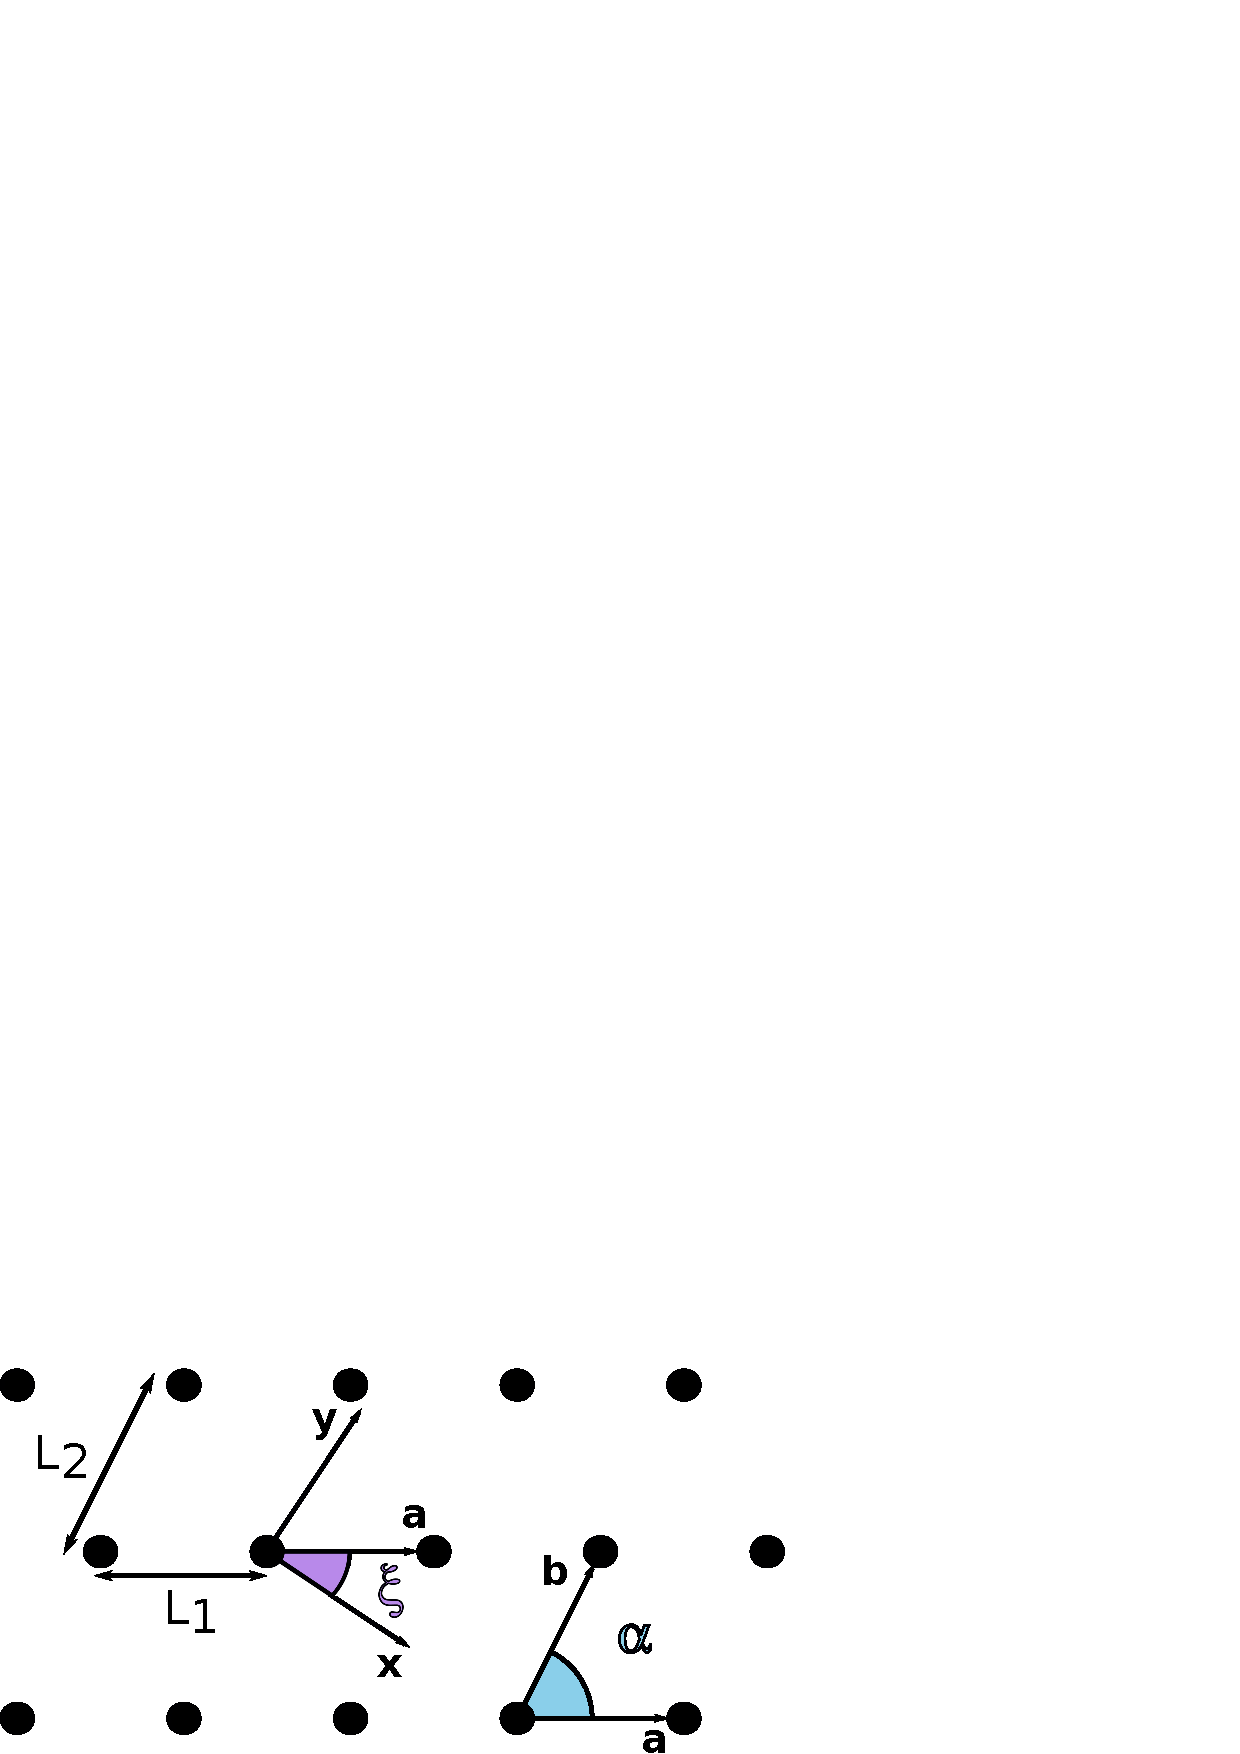
\includegraphics[width=0.5\textwidth]{fig/drawing/2Dlattice.pdf}
\end{center}
\caption{Schematic representation of a 2D lattice (top view). Such a lattice is characterized by lattice lengths $L_1$, $L_2$ and angles $\alpha$ and $\xi$.}
\label{fig:2dlattice}
\end{figure}

Like for the one-dimensional case, a probability distribution function \Code{pdf} has to be defined. One can choose between those listed in Sec.~\ref{baftd} and implements it using \Code{setProbabilityDistribution(pdf)}.

\paragraph{Example} The sample used to run the simulation is made of half-spheres deposited on a substrate. The interference function is "2Dlattice" and the particles are located at the nodes of a square lattice with $L_1=L_2=20$~nm, $\v{a}\equiv \v{b}$ and the probability distribution function is Gaussian. We also use the Decoupling Approximation.

\begin{lstlisting}[language=python, style=eclipseboxed,numbers=none,nolol,caption={\Code{Python} script to define a 2DLattice interference function between hemi-spherical particles as well as the Decoupling Approximation in \Code{getSimulation()}.  The part specific to the interferences is marked in a red italic font.},label={lst:2dlatticeinterf}]
    #collection of particles
    sphere_ff = FormFactorTruncatedSphere(5*nanometer, 5*nanometer)
    sphere = Particle(m_particle, sphere_ff)
    |interference = InterferenceFunction2DLattice(20.0*nanometer, 20.0*nanometer, 90.0*degree, 0.0*degree)|
    |pdf = FTDistribution2DGauss(200.0*nanometer/2.0/M_PI, 75.0*nanometer/2.0/M_PI)|
    |interference.setProbabilityDistribution(pdf)|
    particle_layout = ParticleLayout()
    particle_layout.addParticle(sphere, 1.0)
    |particle_layout.addInterferenceFunction(interference)|

    # interference approx chosen between: DA (default) and SSCA
    |particle_layout.setApproximation(ILayout.DA)|
\end{lstlisting}

%\begin{lstlisting}[language=python, style=eclipseboxed,numbers=none,nolol]
%def get_simulation():
%    """
%    Create and return GISAXS simulation with beam and detector
%    """
%    simulation = Simulation()
%    simulation.setDetectorParameters(100, 0.0*degree, 2.0*degree, 100, 0.0*degree, 2.0*degree, True)
%    simulation.setBeamParameters(1.0*angstrom, 0.2*degree, 0.0*degree)
%    return simulation
%\end{lstlisting}


\begin{figure}[tb]
\begin{center}
\includegraphics[angle=-90,width=0.5\textwidth]{fig/gisasmap/HSphere_2Dlattice.pdf}
\end{center}
\caption{Output intensity scattered from a sample made of half-spheres with 2DLattice interference function in the Decoupling Approximation.}
\label{fig:2dlatticeintensity}
\end{figure}

\FloatBarrier

\newpage%{\cleardoublepage}
%-------------------------------------------------------------------------------
\subsection{InterferenceFunction2DParaCrystal($L_1$, $L_2$, lattice\_angle, $xi$, damping\_length)} % TODO RESTORE \Code{}, \xi
%-------------------------------------------------------------------------------
\begin{itemize}
\item[where] $L_1$, $L_2$ are the lengths of the lattice cell,
\item[] lattice\_angle the angle between the lattice basis vectors $\v{a}, \v{b}$ in direct space,
\item[] $\xi$ is the angle defining the lattice orientation (set to $0$ by default).
\item[] \Code{damping\_length} is used to introduce finite size effects by applying a multiplicative coefficient equal to  $\exp$(-\Code{peak\_distance/damping\_length}) to the Fourier transform of the probability densities. \Code{damping\_length} is equal to 0 by default and, in this case, no correction is applied.
\end{itemize}
Two predefined interference functions can also be used:
\begin{itemize}
\item  \Code{createSquare(peak\_distance, damping\_length, domain\_size\_1, domain\_size\_2)}\\
where the angle between the base vectors of the lattice is set to $\pi/2$,
it creates a squared lattice,
\item \Code{createHexagonal(peak\_distance, damping\_length, domain\_size\_1, domain\_size\_2)}\\
where the angle between the base vectors of the lattice is set to $2\pi/3$ ,
\end{itemize}
where
\Code{domain\_size1, 2} are the dimensions of coherent domains of the paracrystal along the main axes,\\ \Code{peak\_distance} is the same in both directions and $\v{a}\equiv \v{x}$.\\

Probability distribution functions have to be defined. As the two-dimensional paracrystal is defined from two independent one-dimensional paracrystals, we need two of these functions, using\\ \Code{setProbabilityDistributions(pdf\_1, pdf\_2)}, with \Code{pdf\_{1,2}} related to each main axis of the paracrystal (see figure~\ref{fig:2dparaschematic}).


\begin{figure}[tb]
\begin{center}
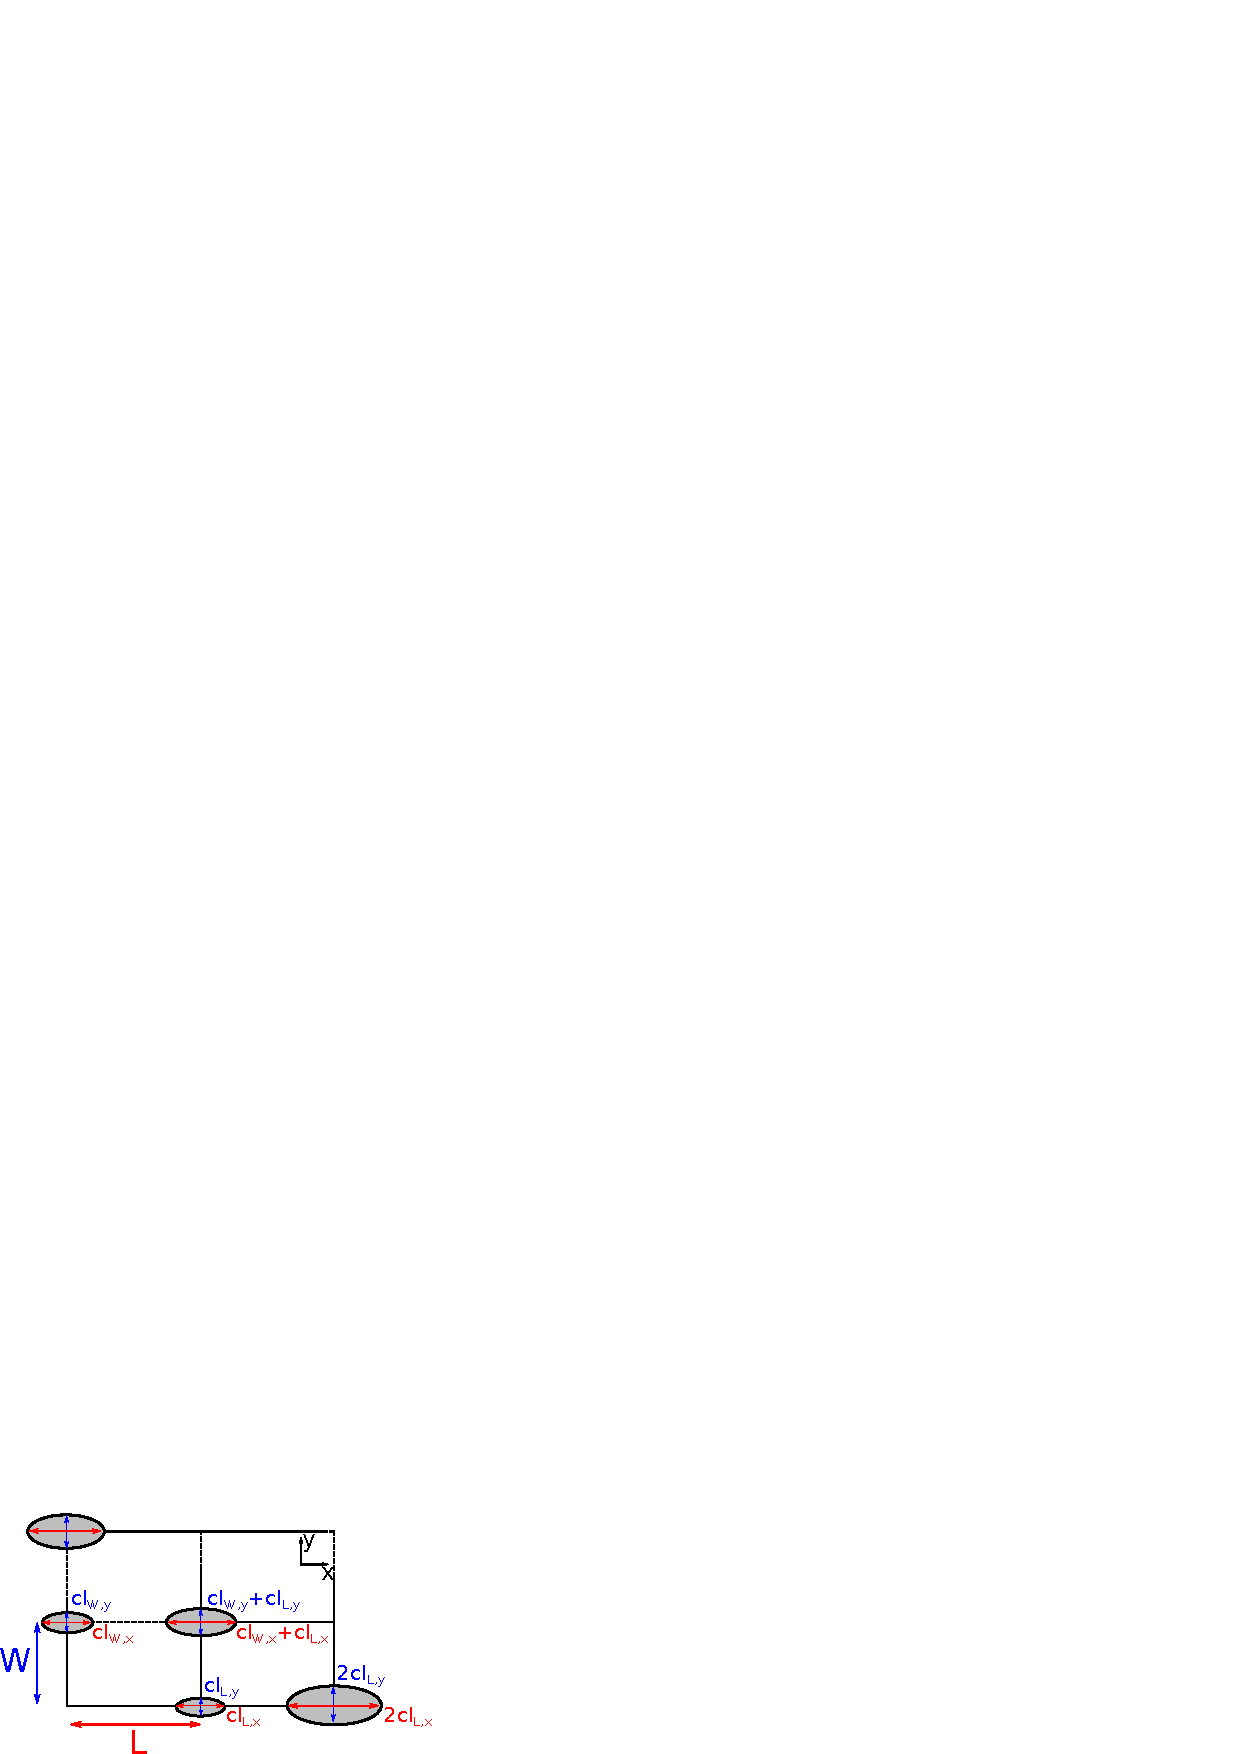
\includegraphics[width=0.75\textwidth]{fig/drawing/drawing2Dparacrystal.pdf}
\end{center}
\caption{Schematics of the ideal 2D paracrystal. The gray-shaded areas mark the regions where the probability to find a node is larger that the width at half-maximum of the distribution. $L$ and  $W$ are the mean inter-node distances along the two crystallographic axes. cl$_{(L,W),(x,y)}$ are the widths of the distribution of distance. The disorder is propagated as we add more nodes. Such a structure would be generated using \Code{InterferenceFunction2DParacrystal(L,W,90.*degrees,0,damp\_length)}, with \Code{pdf$_1$ = FTDistribution2DGauss(cl$_{L,x}$,cl$_{L,y}$)} and  \Code{pdf$_2$ = FTDistribution2DGauss(cl$_{W,x}$,cl$_{W,y}$)}.}
\label{fig:2dparaschematic}
\end{figure}


\paragraph{Example} The particles deposited on a substrate are half-spheres. The scattered beams interference via the 2DParacrystal distribution function. The paracrystal is based on a 2D hexagonal lattice with a Gaussian probability distribution function in reciprocal space.  Script~\ref{lst:2dparainterf} shows the implementation of the interference function and fig.~\ref{fig:2ddl} an example of output intensity using hemi-spherical particles.

\begin{lstlisting}[language=python, style=eclipseboxed,numbers=none,nolol,caption={\Code{Python} script to define a "2DParacrystal" interference function between particles forming an hexagonal monolayer. },label={lst:2dparainterf}]
    interference = InterferenceFunction2DParaCrystal.createHexagonal(30.0*nanometer,0.0, 40.0*micrometer, 40.0*micrometer)|
    pdf = FTDistribution2DCauchy(1.0*nanometer, 1.0*nanometer)
    interference.setProbabilityDistributions(pdf, pdf)
    particle_layout.addInterferenceFunction(interference)
\end{lstlisting}

\begin{figure}[tb]
\begin{center}
\includegraphics[angle=-90,width=0.5\textwidth]{fig/gisasmap/HSphere_2DDL.pdf}
\end{center}
\caption{Output intensity scattered from a sample made of half-spheres with 2DParacrystal interference function.}
\label{fig:2ddl}
\end{figure}

\FloatBarrier


%===============================================================================
\subsection{Summary}
%===============================================================================

\begin{table}[h]
  \footnotesize
\begin{tabular}{lll}
\hline
Function  & Parameters & Comments\\
\hline
\Code{InterferenceFunctionNone}  & None & disordered distribution \\
\hline
\Code{InterferenceFunction1DLattice} & \Code{lattice\_length} & use only with infinitely long/wide particles \\
  & $\xi=\widehat{(\v{x},\v{a})}$ & pdf=(Cauchy, Gauss or Voigt)  to be defined\\
\hline
 \Code{InterferenceFunctionRadialParaCrystal}  & peak\_distance of pdf & pdf=(Cauchy, Gauss or Voigt) to be defined \\
& damping\_length (optional) & \\
\hline
 \Code{InterferenceFunction2DLattice}  & L\_1, L\_2: lattice lengths & pdf=(Cauchy, Gauss or Voigt) to be defined\\
                        & lattice\_angle=$\widehat{(\v{a},\v{b})}$ & \\
                                                            & $\xi =\widehat{(\v{x},\v{a})}$ & \\
\hline
\Code{InterferenceFunction2DParaCrystal}  & L\_1, L\_2: lattice lengths & 2D pdf=(Cauchy, Gauss or Voigt) to be defined \\
                          & lattice\_angle=$\widehat{(\v{a},\v{b})}$ & (1 pdf per axis) \\
& $\xi=\widehat{(\v{x},\v{a})}$ & \\
& damping\_length (optional)  &  same for both axes\\
\hline
\hline
\end{tabular}
\caption{List of interference functions implemented in \BornAgain. pdf : probability distribution function, $\v{a}, \v{b}$ are the lattice base vectors, and $\v{x}$ is the axis vector perpendicular to the detector plane.}
\end{table}

\index{Particle assemblies)}%
\fi

%%\include{Roughness}
%%%%%%%%%%%%%%%%%%%%%%%%%%%%%%%%%%%%%%%%%%%%%%%%%%%%%%%%%%%%%%%%%%%%%%%%%%%%%%%%%%
%%
%%   BornAgain User Manual
%%
%%   homepage:   http://www.bornagainproject.org
%%
%%   copyright:  Forschungszentrum Jülich GmbH 2015
%%
%%   license:    Creative Commons CC-BY-SA
%%
%%   authors:    Scientific Computing Group at MLZ Garching
%%               C. Durniak, M. Ganeva, G. Pospelov, W. Van Herck, J. Wuttke
%%
%%%%%%%%%%%%%%%%%%%%%%%%%%%%%%%%%%%%%%%%%%%%%%%%%%%%%%%%%%%%%%%%%%%%%%%%%%%%%%%%

\chapter{Polarized GISAS}  \label{SPol}

In this chapter,
we generalize our treatment of wave propagation and
grazing-incidence small-angle scattering
to polarized neutrons.
\index{Neutrons!polarized}
\index{Polarization!neutrons}
We therefore need to study spinor wave equations,
in contrast to the scalar theory of the previous chapter.

\MissingSection
\iffalse
%===============================================================================
\section{Polarized neutrons}\label{Snpol}
%===============================================================================


\Work{This is preliminary and incomplete material waiting for revision and extension}


%===============================================================================
\subsection{Wave equation and propagation within one layer}
%===============================================================================

%\cite{Deak_ppt, PhysRevB.76.224420, Deak2001113, PhysRevB.53.6158}.
%\cite{RevModPhys.23.287}

To allow for polarization-dependent interactions,
we replace the squared index of refraction $n^2$
by $1+\uu\chi$, where $\uu\chi$ is a $2\times 2$ susceptibility matrix.
The wave equation \cref{EHomoK} for layer~$l$ becomes
\begin{equation}\label{Ewaveqp}
(\Delta +K^2 +K^2 \uu\chi_l) \u\psi(\r)= 0,
\end{equation}
where $\u\psi(\r)$ is a two-component spinor wavefunction,
with components $\psi_\UP(\r)$ and~$\psi_\DN(\r)$.
At interfaces between layers,
both spinor components of $\u\psi(\r)$ and $\Nabla\u\psi(\r)$
must evolve continuously.

The reasons for the factorization \cref{Ekpar} still apply,
and so we can write
\begin{equation}\label{Ewave3p}
\u\psi(\r) = \u\psi(z) \e^{i \k_\parallel\r_\parallel}.
\end{equation}
As before, $\k_\parallel$ is constant across layers.
The wave equation~\cref{Ewaveqp} reduces to
\begin{equation}\label{Ewavezp}
\left(\partial_z^2 + K^2 + K^2\uu\chi_l - k_\parallel^2 \right) \u\psi(z) = 0.
\end{equation}
We abbreviate
\begin{equation}
  \uu H_l \coloneqq  K^2(1+\uu\chi_l)-k_\parallel^2
\end{equation}
so that the wave equation becomes simply
\begin{equation}\label{Ewaveqp2}
  \left(\partial_z^2 + \uu H_l\right) \u\psi(z) = 0.
\end{equation}
The solution is
\begin{equation}\label{Epsizp}
  \u\psi_l(z)
  = \sum_{k=1}^2 \u x_{l k}\left(\alpha_{l k}\e^{i p_{l k}(z-z_k)}
                            + \beta_{l k}\e^{-i p_{l k}(z-z_k)}\right),
\end{equation}
where the $\u x_{l k}$ are eigenvectors of $\uu H_l$
with eigenvalues $p_{l k}^2$:
\begin{equation}
  \left( -p_{l k}^2 + \uu H_l \right) \u x_{l k} = 0
   \;\text{ for }\;l=1,2.
\end{equation}
In a reproducible algorithm,
the eigenvectors $\u x_{l k}$ must be chosen according to some arbitrary
normalization rule,
for instance
\begin{equation}
  |\u x_{l k}|=1,\quad x_{il\UP} \text{ real and nonnegative}.
\end{equation}
Similarly,
a rule is needed how to handle the case of one degenerate eigenvalue,
which includes in particular the case of scalar interactions.


%-------------------------------------------------------------------------------
\subsection{Wave propagation across layers}
%-------------------------------------------------------------------------------

Generalizing \Cref{Sacrolay},
we introduce the coefficient vector
\begin{equation}
  c_l \coloneqq  {(\alpha_{l1}, \alpha_{l2}, \beta_{l1}, \beta_{l2})}^\text{T}.
\end{equation}
To match solutions for neighboring layers,
continuity is requested for both spinorial components
of $\u\psi$ and $\Nabla\u\psi$.
We have at the bottom of layer~$l$
\begin{equation}\label{EFcFDcp}
  F_l c_l = F_{l+1} D_{l+1} c_{l+1},
\end{equation}
where the matrices are
\begin{equation}
  F_l \coloneqq  \left(\begin{array}{cccc}
    x_{i1\UP}      &x_{i2\UP}     &x_{i1\UP}       &x_{i2\UP}       \\
    x_{i1\DN}      &x_{i2\DN}     &x_{i1\DN}       &x_{i2\DN}       \\
    x_{i1\UP}p_{l1}&x_{i2\UP}p_{l2}&-x_{i1\UP}p_{l1}&-x_{i2\UP}p_{l2}\\
    x_{i1\DN}p_{l1}&x_{i2\DN}p_{l2}&-x_{i1\DN}p_{l1}&-x_{i2\DN}p_{l2}
  \end{array}\right)
\end{equation}
and
\begin{equation}
  D_l \coloneqq  \text{diag}(\delta_{l1}, \delta_{l2}, \delta_{l1}^*, \delta_{l2}^*)
\end{equation}
with the phase factor
\begin{equation}
   \delta_{l k} \coloneqq  \e^{ip_{l k}d_k}.
\end{equation}
Note that matrix $F_l$ has the block form
\begin{equation}
  F_l
  =\left(\begin{array}{ll}\uu x_l&\hphantom{-}\uu x_l\\[1ex]
    \uu x_l\; \uu P_l&-\uu x_l\; \uu P_l\end{array}\right)
    = \uu x_l \cdot
    \left(\begin{array}{cc}\uu 1&\uu 1\\[1ex]
    \uu P_l&-\uu P_l\end{array}\right),
\end{equation}
with
\begin{equation}
  \uu x_l \coloneqq
  \left(\u x_{l1}, \u x_{l2}\right),
  \quad
  \uu P_l \coloneqq
  \text{diag}\left(p_{l1},p_{l2}\right).
\end{equation}
This facilitates the computation of the inverse
\begin{equation}
  F_l^{-1}
    = \frac{1}{2}
    \left(\begin{array}{cc}\uu 1&\hphantom{-}\uu P_l^{-1}\\[1.2ex]
      \uu 1 &-\uu P_l^{-1}\end{array}\right)
      \cdot\uu x_l^{-1},
\end{equation}
which is needed for the transfer matrix $M_l$,
defined as in \cref{EMil}.
With the new meaning of $c_l$ and $M_l$,
the recursion \cref{EcMc} and the explicit solution~\cref{EAtildel}
hold as derived above.
To resolve~\cref{Eci} for the reflected amplitudes $\alpha_{0l}$
as function of the incident amplitudes $\beta_{0l}$,
we choose the notations
\begin{equation}
  \u\alpha_l
  \coloneqq \left(\begin{array}{c}\alpha_{l1}\\\alpha_{l2}\end{array}\right),\quad
  \u\beta_l
  \coloneqq \left(\begin{array}{c}\beta_{l1}\\\beta_{l2}\end{array}\right),\quad
  M\coloneqq M_1 ... M_N % TODO restore \cdots
  \eqqcolon \left(\begin{array}{cc}\uu m_{11}&\uu m_{12}\\
                           \uu m_{21}&\uu m_{22}\end{array}\right),
\end{equation}
where the $\uu m_{l k}$ are $2\times2$ matrices.
Eq.~\cref{Eci} then takes the form
\begin{equation}
  \left(\begin{array}{c}\u\alpha_{0}\\\u\beta_{0}\end{array}\right)
  =
  \left(\begin{array}{cc}\uu m_{11}&\uu m_{12}\\
    \uu m_{21}&\uu m_{22}\end{array}\right)
  \left(\begin{array}{c}\u{0}\\\u\beta_{N}\end{array}\right),
\end{equation}
which immediately yields
\begin{equation}
  \u\alpha_0 = \uu m_{12}\,\uu m_{22}^{-1}\,\u\beta_0.
\end{equation}
\fi

%%%%%%%%%%%%%%%%%%%%%%%%%%%%%%%%%%%%%%%%%%%%%%%%%%%%%%%%%%%%%%%%%%%%%%%%%%%%%%%%
%%
%%   BornAgain User Manual
%%
%%   homepage:   http://www.bornagainproject.org
%%
%%   copyright:  Forschungszentrum Jülich GmbH 2015
%%
%%   license:    Creative Commons CC-BY-SA
%%
%%   authors:    Scientific Computing Group at MLZ Garching
%%               C. Durniak, M. Ganeva, G. Pospelov, W. Van Herck, J. Wuttke
%%
%%%%%%%%%%%%%%%%%%%%%%%%%%%%%%%%%%%%%%%%%%%%%%%%%%%%%%%%%%%%%%%%%%%%%%%%%%%%%%%%

\chapter{Instrument simulation}  \label{SInstr}

%%%%%%%%%%%%%%%%%%%%%%%%%%%%%%%%%%%%%%%%%%%%%%%%%%%%%%%%%%%%%%%%%%%%%%%%%%%%%%%%
\section{Incoming beam and resolution}\label{SBeam}
%%%%%%%%%%%%%%%%%%%%%%%%%%%%%%%%%%%%%%%%%%%%%%%%%%%%%%%%%%%%%%%%%%%%%%%%%%%%%%%%

\MissingSection

%%%%%%%%%%%%%%%%%%%%%%%%%%%%%%%%%%%%%%%%%%%%%%%%%%%%%%%%%%%%%%%%%%%%%%%%%%%%%%%%
\section{Detector images}\label{SdetImg}
%%%%%%%%%%%%%%%%%%%%%%%%%%%%%%%%%%%%%%%%%%%%%%%%%%%%%%%%%%%%%%%%%%%%%%%%%%%%%%%%

\def\tc{\text{c}}

%-------------------------------------------------------------------------------
\begin{figure}[t]
\begin{center}
\includegraphics[width=.5\textwidth]{fig/drawing/experimental_geometry.png}
\end{center}
\caption{Experimental geometry with a two-dimensional pixel detector.}
\label{FexpGeom}
\end{figure}
%-------------------------------------------------------------------------------

To conclude this chapter on the foundations of small-angle scattering,
we shall derive the geometric factors
that allow us to convert differential cross sections into detector counts.
We shall also discuss how to present data on a physically meaningful scale.

%===============================================================================
\subsection{Pixel coordinates, scattering angles, and $\symbf{q}$ components}
%===============================================================================

We assume that scattered radiation is detected in a flat,
two-dimensional detector
that generates histograms on a rectangular grid,
consisting of $n\cdot m$ pixels of constant width and height,
as sketched in \cref{FexpGeom}.
This figure also shows the coordinate system
\index{Conventions|see {Coordinate system}}%
\index{Coordinate system}%
according to unanimous GISAS convention,
with $z$ normal to the sample plane,
and with the incident beam in the $xz$ plane.
The origin is at the center of the sample surface.
We suppose that the detector is mounted perpendicular to the $x$ axis
at a distance $L$ from the sample position.
%the $x$ axis intersects the detector plane at $(L,y_\tc,z_\tc)$.
The real-space coordinate at the center of pixel $(i,j)$ is $(L,y_i,z_i)$.
Each pixel has a width~$\Delta y$ and a height~$\Delta z$.
\index{Detector!pixel coordinate}%
\index{Pixel|see {Detector}}%
BornAgain requires a full parametrization of the detector geometry
\index{Detector!calibration}%
to correctly perform the affine-linear mapping from pixel indices $i,j$
to pixel coordinates $x_i,y_i$;
see the \tuto{141}{rectangular detector tutorial}.
% TODO: link to Detector Reference

Since the differential scattering cross section \cref{Exsectiondef}
is given with respect to a solid-angle element $\d\Omega$,
we need to express the scattered wavevector $\k_\sf$ in spherical coordinates,
using the horizontal azimuth angle~$\phi_\sf$
and the vertical glancing angle $\alpha_\sf$.
The projection of $(\alpha_\sf,\phi_\sf)$ into
the detector plane~$(y,z)$ is known as the \E{gnomonic projection}.
\index{Gnomonic projection}%
\index{Projection!wave vector to pixel coordinate}%
\index{Mapping!wave vector to pixel coordinate}%
\index{Transformation!wave vector to pixel coordinate}%
From elementary trigonometry one finds
\begin{equation}\label{Eyzdet}
  \begin{array}{lcl}
  y &=& L \tan\phi_\sf,\\
  z &=& (L/ \cos\phi_\sf) \tan\alpha_\sf.
  \end{array}
\end{equation}
\cref{Fconstalphi} shows lines of equal $\alpha_\sf$,~$\phi_\sf$
in the detector plane.
To emphasize the curvature of the constant-$\alpha_\sf$ lines,
scattering angles up to more than 25$^\circ$ are shown.
In typical SAS or GISAS,
scattering angles are much smaller,
and therefore the mapping between pixel coordinates and
scattering angles is in a good first approximation linear.
Of course \BornAgain\ is not restricted to this linear regime,
but uses the exact nonlinear mapping~\cref{Eyzdet}.

%-------------------------------------------------------------------------------
\begin{figure}[t]
\begin{center}
\includegraphics[width=.47\textwidth]{fig/drawing/SAS_const_alphi.ps}
\end{center}
\caption{Lines of constant $\alpha_\sf$ (red) or $\phi_\sf$ (blue)
in the detector plane,
for a planar detector at distance~$L$ from the sample.
The black dot indicates the beamstop location for
the central incident beam (SAS geometry, $\hat\k_\si = \hat x$).}
\label{Fconstalphi}
\end{figure}
%-------------------------------------------------------------------------------

To determine the scattering vector $\q_{ij}$
that corresponds to a pixel $(i,j)$,
we need to express the outgoing wavevector~$\k_\sf$ as function of $y$ and~$z$.
This can be done either by inverting \cref{Eyzdet}
and inserting the so obtained $\alpha_\sf(y,z)$ and $\phi_\sf(y)$ in
\begin{equation}\label{Ekf_by_angle}
  \k_\sf=K\left(\begin{array}{c}
   \cos\alpha_\sf\cos\phi_\sf\\
   \cos\alpha_\sf\sin\phi_\sf\\
   \sin\alpha_\sf\end{array}\right),
\end{equation}
or much more directly by using geometric similarity in Cartesian coordinates.
The result is rather simple:
\Emph{
\begin{equation}\label{Ekf_by_pixel}
  \k_\sf=\frac{K}{\sqrt{L^2+y^2+z^2}}\left(\begin{array}{c}
   L\\
   y\\
   z\end{array}\right).
\end{equation}
\vspace*{-5pt}}


%-------------------------------------------------------------------------------
\begin{figure}[t]
\begin{center}
\includegraphics[width=.47\textwidth]{fig/drawing/SAS_const_q_x.ps}
\hfill
\includegraphics[width=.47\textwidth]{fig/drawing/SAS_const_q_yz.ps}
\end{center}
\caption{Lines of constant $q_x$ (left), $q_y$ or $q_z$ (right),
in units of the incident wavenumber $K=2\pi/\lambda$,
for a planar detector.
SAS geometry as in Fig.~\protect\ref{Fconstalphi}.}
\label{Fconstq}
\end{figure}
%-------------------------------------------------------------------------------

The transform \cref{Eqalgo} between pixel coordinates $y$,~$z$
and physical scattering vector components $q_y$, $q_z$
is nonlinear, due to the square-root term in the denominator of~\cref{Ekf_by_pixel}.
For $y,z\ll L$, however, nonlinear terms loose importance.

%-------------------------------------------------------------------------------
\begin{figure}[t]
\begin{center}
\includegraphics[width=1\textwidth]{fig/ff2/ff_det_box.pdf}
\end{center}
\caption{Simulated detector image for small-angle scattering from
uncorrelated cuboids (right rectangular prisms).
  \index{Box (form factor)}
  \index{Cuboid (form factor)}
  \index{Prism (form factor)!reactangular (Box)}
  \index{FormFactorBox@\Code{FormFactorBox}}
The incoming wavelength is 0.1~nm.
The prisms have edge lengths $L_y=L_z=10$~nm;
the length $L_x$, in beam direction, is varied as shown above the plots.
\index{Circular modulation}%
The circular modulation comes from a factor $\sinc(q_x L_x/2)$
in the cuboid form factor, with $q_x$ given by~\cref{Eqxasy}.}
\label{Fdetbox}
\end{figure}
%-------------------------------------------------------------------------------

The left detector frame in \cref{Fconstq}
shows circles of constant values of $\pm q_x$.
For given steps in $q_x$, the distance between adjacent circles
increases towards the detector center.
From \cref{Eq} and \cref{Ekf_by_pixel},
one finds asymptotically for $y,z\to L$
that $q_x$ goes with the square of the two other components of the scattering vector,
\begin{equation}\label{Eqxasy}
  \frac{q_x}{K}
  \doteq \frac{y^2+z^2}{2 L^2}
  \doteq \frac{q_y^2 + q_z^2}{2K^2}.
\end{equation}
Therefore, under typical small angle conditions $y,z\to L$
the dependence of the scattering signal on $q_x$ is unimportant:
one basically measures $v(\q)\simeq v(0,q_y,q_z)$.
The exception, for sample structures with long correlations in $x$~direction,
is illustrated in~\cref{Fdetbox}.

%-------------------------------------------------------------------------------
\begin{figure}[t]
\begin{center}
\includegraphics[width=.47\textwidth]{fig/drawing/SAS_const_p_yz.ps}
\end{center}
\caption{The outer contour of the blue and red grid
shows the border of a square detector image
after transformation into the physical coordinates $q_y$,~$q_z$.
The blue and red curves correspond to horizontal and vertical lines in the detector.}
\label{Fconstp}
\end{figure}
%-------------------------------------------------------------------------------

As anticipated in \cref{Eqxasy},
the other two components of $\q$ are in first order linear in the pixel coordinates,
\begin{equation}
  \frac{q_y}{K}=\frac{y}{L}\left(1-\frac{y^2+z^2}{2L^2}+\ldots\right),
\end{equation}
and similarly for~$q_z$.
The nonlinear correction terms lead to the pincushion distortion
shown in the right detector frame in \cref{Fconstq}.
\index{Distortion!of $q_x$, $q_y$ grid in detector plane}%
\index{Detector!distortion of $q_x$, $q_y$ grid}%
\index{Pincushion distortion}%

Since pixel coordinates are meaningful only
with respect to a specific experimental setup,
users may wish to transform detector images
towards the physical coordinates $q_y$ and~$q_z$.
As shown in \cref{Fconstp},
this would yield a barrel-shaped illuminated area
in the $q_y$,~$q_z$~plane.

To summarize this section,
the wavevector $\q_{ij}$ can be determined from the pixel indices
through the following steps:
\begin{equation}\label{Eqalgo}
  \begin{array}{cl}
      (i,j)&\\
      \downarrow&\mbox{calibrate of origin, then employ affine-linear mapping}\\
      (y,z)\\
      \downarrow&\mbox{use (\protect\ref{Ekf_by_pixel})}\\
      \k_\sf&\\
      \downarrow&\mbox{use (\protect\ref{Eq})}\\
      \q&\\
  \end{array}
\end{equation}

\Note{\indent Transforming detector images
  from pixel coordinates into the $q_y$,~$q_z$~plane is not implemented in \BornAgain,
  and not on our agenda.
  We would, however, like to hear about use cases.}

\Emph{\indent When simulating and fitting experimental data with \BornAgain,
detector images remain unchanged.
All work is done in terms of reduced pixel coordinates $y/L$ and~$z/L$.
Corrections are applied to the simulated, not to the measured data.}

\Work{\indent \ldots show how to plot $q$ grid on top of detector image \ldots}

%===============================================================================
\subsection{Intensity transformation}
%===============================================================================

The solid angle under which a detector pixel
is illuminated from the sample is in linear approximation
\begin{equation}
  \Delta\Omega
  = \cos\alpha_\sf\:\Delta\alpha_\sf\,\Delta\phi_\sf
  = \cos\alpha_\sf
    \left|\frac{\partial(\alpha_\sf,\phi_\sf)}{\partial(y,z)}\right|
    \Delta y \,\Delta z
  = \cos^3\!\alpha_\sf\, \cos^3\!\phi_\sf\: \frac{\Delta y \,\Delta z}{L^2}.
\end{equation}
\index{Detector!illumination angle correction factor}%
\index{Illumination!detector}%
Altogether,
the expected count rate in detector pixel $(i,j)$ is proportional to
\begin{equation}\label{EItrafo_cos}
  I_{ij} = \cos^3\!\alpha_\sf\, \cos^3\!\phi_\sf\:
          \frac{\partial\sigma}{\partial\Omega}(\q_{ij}),
\end{equation}
where we have omitted constant factors $L^{-2}$, $\Delta y$ and $\Delta z$.
Using pixel coordinates instead of angles, this can be rewritten as
\Emph{%
\begin{equation}\label{EItrafo_pix}
  I_{ij} = \left( 1+\frac{y^2+z^2}{L^2}\right)^{-3/2}
          \frac{\partial\sigma}{\partial\Omega}\bigl(\q_{ij}(y,z)\bigr).
\end{equation}
\vspace*{-2pt}}
%(usually as the centre between the transmitted
%and the specularly reflected beam spot).

%Tradition wants that raw data be \E{treated} or \E{reduced}
%before they are \E{analyzed}.
%In our case, raw data reduction would comprise
%the transform \cref{Eqalgo} of pixel coordinates into scattering vectors,
%and the accompanying renormalization \cref{EItrafo} of pixel counts.


%%%%%%%%%%%%%%%%%%%%%%%%%%%%%%%%%%%%%%%%%%%%%%%%%%%%%%%%%%%%%%%%%%%%%%%%%%%%%%%%%
%%
%%   BornAgain User Manual
%%
%%   homepage:   http://www.bornagainproject.org
%%
%%   copyright:  Forschungszentrum Jülich GmbH 2016
%%
%%   license:    Creative Commons CC-BY-SA
%%
%%   authors:    Scientific Computing Group at MLZ Garching
%%               M. Ganeva, G. Pospelov, W. Van Herck, J. Wuttke
%%
%%%%%%%%%%%%%%%%%%%%%%%%%%%%%%%%%%%%%%%%%%%%%%%%%%%%%%%%%%%%%%%%%%%%%%%%%%%%%%%%

\newpage
\chapter{The three interfaces of \BornAgain}  \label{sec:API3}

The core of \BornAgain\
\index{Core|see {\Code{libBornAgainCore}}}
For a given model,
\BornAgain\ provides an efficient computation of the expected detector image.
Furthermore \BornAgain\ comes with various minimizers that optimize model parameters
to fit the simulated detector image to a given experimental image.

All this functionality is implemented in a library, \Code{libBornAgainCore}.
\index{libBornAgainCore@\Code{libBornAgainCore}}
This library, in turn, depends on a number of other libraries,
as indicated in \cref{Farchi}.
One of these libraries, the minimizer wrapper \Code{libBornAgainFit}
\index{libBornAgainFit@\Code{libBornAgainFit}}
\index{Minimizers|see \Code{libBornAgainFit}}
has been written specifically for use in \BornAgain,
and for the time being is only distributed as part of \BornAgain,
though in the future it may find applications in other contexts.
The other library dependences of \Code{libBornAgainCore}
are multi-purpose libraries that are easily available as open-source packages.
\index{Dependences!libraries}

%%%%%%%%%%%%%%%%%%%%%%%%%%%%%%%%%%%%%%%%%%%%%%%%%%%%%%%%%%%%%%%%%%%%%%%%%%%%%%%%%
%%
%%   BornAgain User Manual
%%
%%   homepage:   http://www.bornagainproject.org
%%
%%   copyright:  Forschungszentrum Jülich GmbH 2015
%%
%%   license:    Creative Commons CC-BY-SA
%%
%%   authors:    Scientific Computing Group at MLZ Garching
%%               C. Durniak, M. Ganeva, G. Pospelov, W. Van Herck, J. Wuttke
%%
%%%%%%%%%%%%%%%%%%%%%%%%%%%%%%%%%%%%%%%%%%%%%%%%%%%%%%%%%%%%%%%%%%%%%%%%%%%%%%%%

\def\PyImport#1{%
\lstinputlisting[language=python,style=eclipseboxed,name=ex1,nolol]{../../Examples/python/#1}}

\newpage
\chapter{Using the Python API}  \label{sec:Usage}


%%%%%%%%%%%%%%%%%%%%%%%%%%%%%%%%%%%%%%%%%%%%%%%%%%%%%%%%%%%%%%%%%%%%%%%%%%%%%%%%
\section{Running a simulation}
%%%%%%%%%%%%%%%%%%%%%%%%%%%%%%%%%%%%%%%%%%%%%%%%%%%%%%%%%%%%%%%%%%%%%%%%%%%%%%%%

A simulation of GISAS using \BornAgain\ consists of the following steps:
\begin{itemize}
\item define materials by specifying name and refractive index,
\item define layers by specifying thickness, roughness, material,
\item define embedded particles by specifying shape, size,
   constituting material, interference function,
\item embed the particles in layers, specifying density, position, orientation,
\item assemble a multilayered sample,
\item specify input beam and detector characteristics,
\item run the simulation,
\item save the simulated detector image.
\end{itemize}

\noindent
All these steps can be organized in either a Graphical User Interface (GUI) or by providing a Python script with the simulation description.
In the following, we describe how to write a
\Code{Python} script which runs a \BornAgain\ simulation. For tutorials about this programming language, the users are referred to \cite{Lut09}.


% More information about the general software architecture and \BornAgain\ internal design are given in \cref{sec:SoftwareArchitecture}.


%===============================================================================
\subsection{Units:}
%===============================================================================
\index{Units}

By default the angles are expressed in radians and the lengths are given in
nanometers.  But it is possible to use other units by
specifying them right after the value of the corresponding
parameter like, for example, \Code{20.0*micrometer}.


%===============================================================================
\subsection{A first example} \label{sec:Example1Python}
%===============================================================================

In this example, we simulate the scattering from a mixture of
cylindrical and prismatic nanoparticles without any interference
between them. These particles are placed in air, on top
of a substrate.\\ We are going to go through each step of the
simulation. The Python code snippet specific to each stage will be given at
the beginning of the description.
More examples can be found at our project web site \url{http://www.bornagainproject.org/documentation/python_examples}

% But for the sake of completeness the full code is given
% in \cref{PythonSimulationExampleScript}.

%-------------------------------------------------------------------------------
\subsubsection{Importing Python modules}
%-------------------------------------------------------------------------------

\setPy
\begin{lstlisting}
import numpy @\label{import_lib_beg}@
import matplotlib
import pylab @\label{import_lib_end}@
from bornagain import * @\label{import_ba}@
\end{lstlisting}
We start by importing different functions from external
modules, for example \Code{NumPy} (lines~\ref{import_lib_beg}-\ref{import_lib_end}), which
is a fundamental package for scientific computing with Python
\cite{s:numpy}.  In particular, line~\ref{import_ba}
imports the features of \BornAgain\ software.

%-------------------------------------------------------------------------------
\subsubsection{Defining the materials}
%-------------------------------------------------------------------------------

\begin{lstlisting}
def get_sample(): @\label{def_function}@
    """
    Build and return the sample representing cylinders and pyramids on top of substrate without interference.
   """
    # defining materials @\label{material1}@
    m_air = HomogeneousMaterial("Air", 0.0, 0.0)  @\label{material2}@
    m_substrate = HomogeneousMaterial("Substrate", 6e-6, 2e-8) @\label{material3}@
    m_particle = HomogeneousMaterial("Particle", 6e-4, 2e-8) @\label{materialparticle}@

\end{lstlisting}
Line~\ref{def_function} marks the beginning of the
function to define our sample. Lines~\ref{material2}, \ref{material3} and \ref{materialparticle} define different
materials using class \Code{HomogeneousMaterial}. The general syntax is the following
\begin{lstlisting}
<material_name> = HomogeneousMaterial("name", delta, beta)
\end{lstlisting}
where \Code{name} is the name of the
material associated with its complex refractive index
n=1-\Code{delta} +i \Code{beta}. \Code{<material\_name>} is later used when
referring to this particular material. The three materials defined in this example are \Code{Air} with a refractive
index of 1 (\Code{delta = beta = 0}), a \Code{Substrate} associated with a complex refractive index
equal to $1-6\times 10^{-6} +i2\times 10^{-8} $, and the material of the particles, whose refractive index is \Code{n}$=1-6\times 10^{-4}+i2\times 10^{-8}$.

%-------------------------------------------------------------------------------
\subsubsection{Defining the particles}
%-------------------------------------------------------------------------------
\begin{lstlisting}
    # collection of particles @\label{particles1}@
    cylinder_ff = FormFactorCylinder(5*nanometer, 5*nanometer) @\label{particlescyl1}@
    cylinder = Particle(m_particle, cylinder_ff) @\label{particlescyl2}@
    prism_ff = FormFactorPrism3(10*nanometer, 5*nanometer) @\label{particlesprism1}@
    prism = Particle(m_particle, prism_ff) @\label{particlesprism2}@
\end{lstlisting}
We implement two different shapes of particles: cylinders and
prisms (\idest  elongated particles with a constant equilateral triangular cross section).

All particles implemented in \BornAgain\ are defined by their
form factors (see \cref{SFF}), their sizes and the material
they are made of. Here, for the
cylindrical particle, we input its radius and height.  For the prism,
the possible inputs are the length of one side of its equilateral triangular
base and its height.

In order to define a particle, we proceed in two steps. For example for
the cylindrical particle, we first specify the form factor of a cylinder with
its radius and height, both equal to 5 nanometers in this particular
case (see line~\ref{particlescyl1}). Then we associate this shape with
the constituting material as in line~\ref{particlescyl2}.
The same procedure has been applied for the prism in lines~\ref{particlesprism1} and \ref{particlesprism2}, respectively.

%-------------------------------------------------------------------------------
\subsubsection{Characterizing particles assembly}
%-------------------------------------------------------------------------------
\begin{lstlisting}
    particle_layout = ParticleLayout()  @\label{particlesdecor1}@
    particle_layout.addParticle(cylinder, 0.5)  @\label{particlesdecor2}@
    particle_layout.addParticle(prism, 0.5)@\label{particlesdecor3}@
    interference = InterferenceFunctionNone()  @\label{particlesnointerf}@
    particle_layout.addInterferenceFunction(interference)  @\label{particlesinterf}@
\end{lstlisting}
The object which holds the information about the positions and densities of particles
in our sample is called \Code{ParticleLayout}
(line~\ref{particlesdecor1}). We use the associated function \Code{addParticle}
for each particle shape (lines~\ref{particlesdecor2}, \ref{particlesdecor3}). Its general syntax is

\begin{lstlisting}addParticle(<particle_name>, abundance)
\end{lstlisting}
where \Code{<particle\_name>} is the name used to define the particles
(lines~\ref{particlescyl2} and \ref{particlesprism2}) and
\Code{abundance} is the proportion of this type of particles,
normalized to the total number of particles. Here we have 50\% of cylinders
and 50\% of prisms.

\noindent Finally, lines~\ref{particlesnointerf} and
\ref{particlesinterf} specify that there is \textbf{no coherent interference} between
the waves scattered by these particles. In this case, the intensity is calculated by
the incoherent sum of the scattered waves: $\bra |F_j|^2\ket$,
where $F_j$ is the form factor associated with the particle of type $j$.  The way these waves
interfere imposes the horizontal distribution of
the particles as
the interference reflects the long or short-range order of the
particles distribution (see  \cref{sec:sect:interf}). On the contrary, the vertical position is
imposed when we add the particles in a given layer by parameter \Code{depth}, as shown in lines~\ref{particlesdecor2} and \ref{particlesdecor3}.

%-------------------------------------------------------------------------------
\subsubsection{Multilayer}
%-------------------------------------------------------------------------------
\begin{lstlisting}
# air layer with particles and substrate form multi layer  @\label{sampleassembling}@
    air_layer = Layer(m_air) @\label{airlayer}@
    air_layer.addLayout(particle_layout) @\label{airlayerdecorator}@
    substrate_layer = Layer(m_substrate, 0)  @\label{substratelayer}@
    multi_layer = MultiLayer() @\label{multilayercanvas}@
    multi_layer.addLayer(air_layer) @\label{layerairdecor}@
    multi_layer.addLayer(substrate_layer) @\label{layersubstrate}@
    return multi_layer @\label{returnmlayer}@
\end{lstlisting}
We now have to configure our sample. For this first example,
the particles, \idest  cylinders and prisms, are on top of a substrate in an
air layer. \textbf{The order in which we define these layers is important: we
start from the top layer down to the bottom one}.

Let us start with the air layer. It contains the particles. In
line~\ref{airlayer}, we use the previously defined \Code{m\_air}
(="air" material) (line~\ref{material2}). The command in line~\ref{airlayerdecorator} shows that this layer contains particles
which are defined using particle layout object. The substrate layer
only contains the substrate material (line~\ref{substratelayer}).
%Note that the
%\Code{depth} is referenced to the bottom of the top layer (negative
%values would correspond to particles floating above layer 1 as
%the vertical axis is pointing upwards).

There are different possible syntaxes to define a layer. As shown in
lines~\ref{airlayer} and \ref{substratelayer}, we can use
\Code{Layer(<material\_name>,thickness)} or
\Code{Layer(<material\_name>)}. The second case corresponds
to the default value of the \Code{thickness}, equal to 0. The \Code{thickness} is
expressed in  nanometers.

Our two layers are now fully characterized. The sample is assembled using
\Code{MultiLayer()} constructor (line~\ref{multilayercanvas}): we start with the air layer decorated
with the particles (line~\ref{layerairdecor}), which is the layer at
the top and end with the bottom layer, which is the
substrate (line~\ref{layersubstrate}).

%-------------------------------------------------------------------------------
\subsubsection{Characterizing the input beam and output detector}
%-------------------------------------------------------------------------------

\begin{lstlisting}
def get_simulation():  @\label{run1}@
    """
    Create and return GISAXS simulation with beam and detector defined
    """
    simulation = Simulation() @\label{run2}@
    simulation.setDetectorParameters(100, -1.0*degree, 1.0*degree, 100, 0.0*degree, 2.0*degree) @\label{rundetector}@
    simulation.setBeamParameters(1.0*angstrom, 0.2*degree, 0.0*degree) @\label{runbeam}@
    return simulation @\label{returnsimul}@
\end{lstlisting}
The first stage is to create the \Code{Simulation()} object (line~\ref{run2}). Then we define the detector (line~\ref{rundetector}) and beam
parameters (line~\ref{runbeam}). %, which are associated with the
%sample previously defined (line~\ref{runsample}). Finally we run
%the simulation (line~\ref{runsimul}).
Those functions are part of the Simulation class.
The different incident and exit angles are shown in \cref{fig:multil3d}.

The detector parameters are set using ranges of angles via
the function:

\begin{lstlisting}
setDetectorParameters(n_phi, phi_f_min, phi_f_max, n_alpha, alpha_f_min, alpha_f_max),
\end{lstlisting}


\noindent where number of bins \Code{n\_phi}, low edge of first bin \Code{phi\_f\_min} and
upper edge of last bin \Code{phi\_f\_max} all together define $\phi_f$ detector axis,
while \Code{n\_alpha}, \Code{alpha\_f\_min} and \Code{alpha\_f\_max} are related to
$\alpha_f$ detector axis.

\Note{Axis binning:
By default axes are binned to provide constant bin size in k-space, which means slightly
non-equidistant binning in angle space. Other possible options, including user defined
axes with custom variable bin size are explained elsewhere.}

%are the minimum and maximum values of $\phi_f$, respectively, \Code{n\_alpha} is
%the number of bins for $\alpha_f$ axis, \Code{alpha\_f\_min} and \Code{alpha\_f\_max}
%are the minimum and maximum values of
%$\alpha_f$, respectively.

%\Code{isgisaxs\_style=True} (default value = \Code{False}) is a boolean
%used to characterise the structure of the output data. If
%\Code{isgisaxs\_style=True}, the output data is binned at constant
%values of the sine of the output angles, $\alpha_f$ and $\phi_f$, otherwise it is binned
%at constant values of these two angles.\\

\noindent To characterize the beam we use function
\begin{lstlisting}
setBeamParameters(lambda, alpha_i, phi_i),
\end{lstlisting}

\noindent where \Code{lambda} is the incident beam wavelength,
\Code{alpha\_i} is the incident
grazing angle on the surface of the sample,
\Code{phi\_i} is the in-plane
direction of the incident beam (measured with respect to the $x$-axis).


%-------------------------------------------------------------------------------
\subsubsection{Running the simulation and plotting the results}
%-------------------------------------------------------------------------------

\begin{lstlisting}
def run_simulation(): @\label{run_simulation}@
    """
   Run simulation and plot results
    """
    sample = get_sample() @\label{get_sample}@
    simulation = get_simulation() @\label{get_simulation}@
    simulation.setSample(sample)  @\label{setsample}@
    simulation.runSimulation()  @\label{runsimul}@
    result = simulation.getIntensityData().getArray() + 1  # for log scale  @\label{outputdata}@
    pylab.imshow(numpy.rot90(result, 1), norm=matplotlib.colors.LogNorm(), extent=[-1.0, 1.0, 0, 2.0]) @\label{plot1}@
    pylab.show() @\label{plot2}@
\end{lstlisting}
%In function \Code{run\_simulation()}, we associate the sample
%characterised by function \Code{get\_sample()} with the input beam and
%output detector, defined in function \Code{get\_simulation()} (line~\ref{runsample}).
The function, whose definition starts from line~\ref{run_simulation}, gathers all
items. We create the sample and the simulation objects at the lines
~\ref{get_sample} and \ref{get_simulation}, using calls to the previously defined functions. We assign the sample to the simulation at line ~\ref{setsample} and
finally launch the simulation at line ~\ref{runsimul}.

In line~\ref{outputdata} we obtain the simulated intensity
as a function of outgoing angles $\alpha_f$ and $\phi_f$ for further
uses (plots, fits,\ldots) as a \Code{NumPy} array containing
\Code{n\_phi}$\times$\Code{n\_alpha}
datapoints. Lines~\ref{plot1}-\ref{plot2} produces the two-dimensional
contour plot of the intensity as a function of $\alpha_f$ and
$\phi_f$ shown in \cref{fig:output_ex1}.

\begin{figure}[htbp]
  \begin{center}
   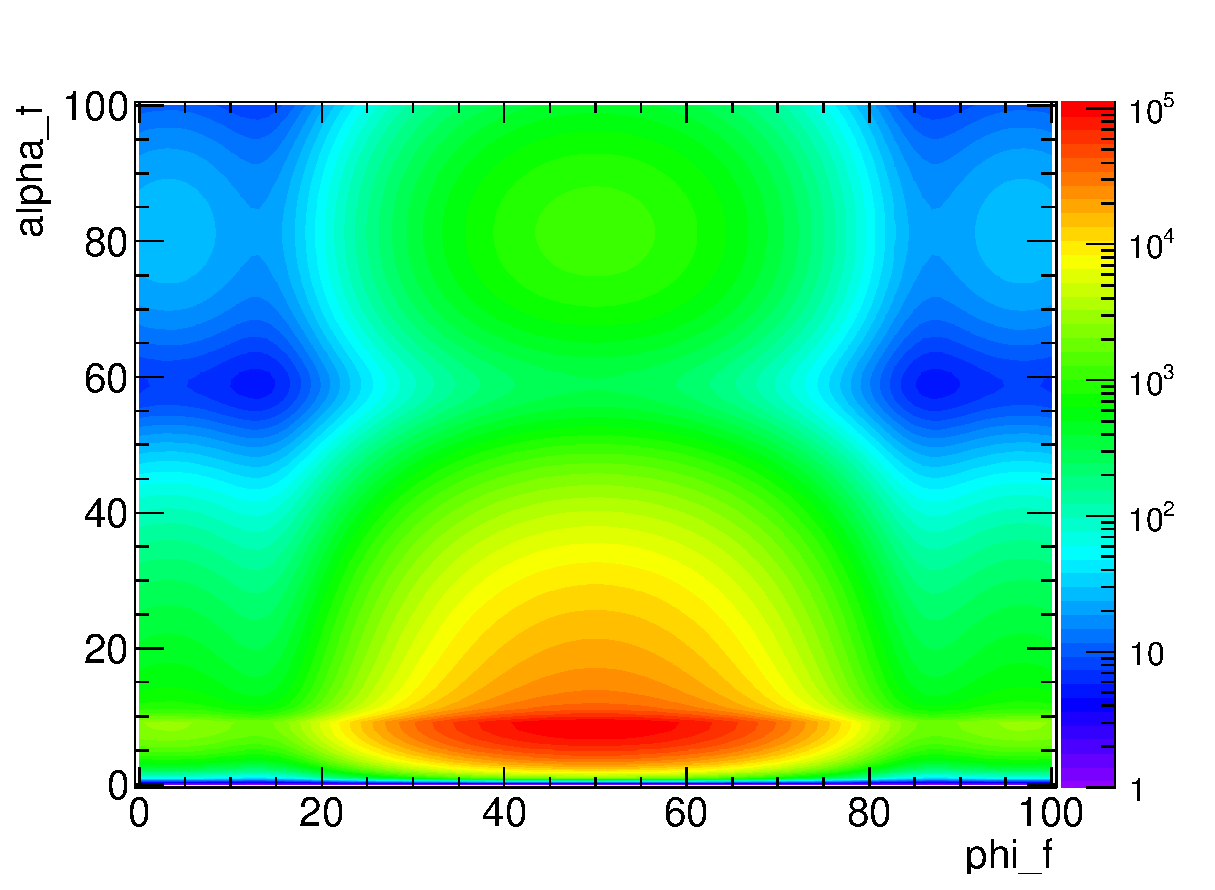
\includegraphics[clip=true, width=120mm]{fig/gisasmap/Manual_ex1.eps}
  \end{center}
  \caption[Example 1: Simulated grazing-incidence small-angle X-ray scattering from a mixture of
cylindrical and prismatic nanoparticles without any interference, deposited on top
of a substrate]{Simulated grazing-incidence small-angle X-ray scattering from a mixture of
cylindrical and prismatic nanoparticles without any interference, deposited on top
of a substrate. The input beam is characterized by a wavelength
$\lambda$ of 1~\AA\ and incident angles $\alpha_i=0.2^{\circ}$, $\phi_i=0^{\circ}$. The
cylinders have a radius and a height both equal to 5~nm, the prisms
are characterized by a side length equal to 10~nm and they are 5~nm high. The
material of the particles has a refractive index of $1-6\times 10^{-4}+i2\times 10^{-8}$. For the substrate
it is equal to $1-6\times 10^{-6} +i2\times 10^{-8} $. The color scale
is associated with the output intensity in arbitrary units. }
\label{fig:output_ex1}
\end{figure}


%===============================================================================
\subsection{Working with sample parameters}
   \label{sec:WorkingWithSampleParameters}
%===============================================================================


This section gives additional details about the manipulation of sample parameters
during run time; that is after the sample has already been constructed.
For a single simulation this is normally not necessary. However it might be useful
during interactive work when the user tries to find optimal sample parameters by
running a series of simulations.
A similar task also arises when the theoretical model, composed of the
description of the sample and of the simulation, is used for fitting real data.
In this case, the fitting kernel requires a list of the existing sample parameters
and a mechanism for changing the values of these parameters in order to find
their optima.

In \BornAgain\ this is done using the so-called sample parameter pool
mechanism. We are going to briefly explain this approach using the example
of \cref{sec:Example1Python}.

In \BornAgain\ a sample is described by a hierarchical tree of objects.
For the multilayer created in the previous section this tree can be graphically
represented as shown in \cref{fig:sample_tree}. Similar trees can
be printed in a Python
session by running \Code{multi\_layer.printSampleTree()}

\begin{figure}[p!]

\tikzstyle{every node}=[draw=black,thick,anchor=west]
\tikzstyle{selected}=[draw=red,fill=red!30]
\tikzstyle{optional}=[dashed,fill=gray!50]
\begin{tikzpicture}[%
  grow via three points={one child at (0.5,-0.7) and
  two children at (0.5,-0.7) and (0.5,-1.4)},
  edge from parent path={(\tikzparentnode.south) |- (\tikzchildnode.west)}]
  \node {MultiLayer}
    child { node {Layer \#0}
		child { node {ParticleLayout }
			child { node {Particle Info 0}
				child {node {Particle }
					child { node {FormFactorCylinder}
						child { node [optional] { radius:5.0} }
						child { node [optional] { height:5.0} }
					}
				}
    			child [missing] {}
    			child [missing] {}
			    child [missing] {}
				child {node [optional] { abundance:0.5} }
				child {node [optional] { depth:0.0} }
			}
    		child [missing] {}
    		child [missing] {}
			child [missing] {}
    		child [missing] {}
    		child [missing] {}
			child [missing] {}
			child { node {Particle Info 1}
				child {node {Particle }
					child { node {FormFactorPrism3}
						child { node [optional] { length:10.0} }
						child { node [optional] { height:5.0} }
					}
				}
    			child [missing] {}
    			child [missing] {}
			    child [missing] {}
				child {node [optional] { abundance:0.5} }
				child {node [optional] { depth:0.0} }
			}
		}
		child [missing] {}
   		child [missing] {}
	    child [missing] {}
		child [missing] {}
   		child [missing] {}
	    child [missing] {}
	    child [missing] {}
		child [missing] {}
   		child [missing] {}
	    child [missing] {}
		child [missing] {}
   		child [missing] {}
	    child [missing] {}
	    child [missing] {}
		child {node [optional] { thickness:0.0} }
    }
	child [missing] {}
   	child [missing] {}
	child [missing] {}
   	child [missing] {}
	child [missing] {}
	child [missing] {}
   	child [missing] {}
	child [missing] {}
   	child [missing] {}
	child [missing] {}
	child [missing] {}
   	child [missing] {}
	child [missing] {}
   	child [missing] {}
	child [missing] {}
	child [missing] {}
	child { node {Layer interface \#0}
    	child {node { roughness}
    		child {node [optional] { corrlength:0.0} }
    		child {node [optional] { hurst:0.0} }
    		child {node [optional] { sigma:0.0} }
    	}
	}
   	child [missing] {}
	child [missing] {}
	child [missing] {}
    child { node {Layer \#1}
    	child {node [optional] { thickness:0.0} }
    }
	child [missing] {}
    child { node [optional] {CrossCorrLength:0.0} };

\end{tikzpicture}
\caption{Tree representation of the sample structure.}
\label{fig:sample_tree}
\end{figure}


The top \Code{MultiLayer} object is composed of three children, namely
\Code{Layer \#0, Layer Interface \#0} and \Code{Layer \#1}. The
children objects might themselves also be decomposed into tree-like structures. For example,
\Code{Layer \#0} contains a \Code{ParticleLayout} object, which holds information
related to the two types of particles populating the layer. All numerical values used
during the sample construction (thickness of layers, size of particles, roughness parameters) are part of the same tree structure.
They are marked in the figure with shaded gray boxes.

These values are registered in the sample parameter pool using the name
composed of the corresponding nodes' names. And they can be accessed/changed
during run time. For example, the \Code{height} of the cylinders
populating the first layer can be changed from the
current value of $5~\rm{nm}$ to $1~\rm{nm}$ by running the command

\begin{lstlisting}[language=shell, style=commandline]
multi_layer.setParameterValue('/MultiLayer/Layer0/ParticleLayout/ParticleInfo0/Particle/FormFactorCylinder/height', 1.0)
\end{lstlisting}


A list of the names and values of all registered sample's parameters
can be displayed using the command

\begin{lstlisting}[language=shell, style=commandline]
> multi_layer.printParameters()
The sample contains following parameters ('name':value)
'/MultiLayer/Layer0/ParticleLayout/ParticleInfo0/Particle/FormFactorCylinder/height':5
'/MultiLayer/Layer0/ParticleLayout/ParticleInfo0/Particle/FormFactorCylinder/radius':5
'/MultiLayer/Layer0/ParticleLayout/ParticleInfo0/abundance':0.5
'/MultiLayer/Layer0/ParticleLayout/ParticleInfo0/depth':0
'/MultiLayer/Layer0/ParticleLayout/ParticleInfo1/Particle/FormFactorPrism3/length':5
'/MultiLayer/Layer0/ParticleLayout/ParticleInfo1/Particle/FormFactorPrism3/height':5
'/MultiLayer/Layer0/ParticleLayout/ParticleInfo1/abundance':0.5
'/MultiLayer/Layer0/ParticleLayout/ParticleInfo1/depth':0
'/MultiLayer/Layer0/thickness':0
'/MultiLayer/Layer1/thickness':0
'/MultiLayer/LayerInterface/roughness/corrlength':0
'/MultiLayer/LayerInterface/roughness/hurst':0
'/MultiLayer/LayerInterface/roughness/sigma':0
'/MultiLayer/crossCorrLength':0
\end{lstlisting}

Wildcards \Code{'*'} can be used to reduce typing or to work on a group
of parameters. In the example below, the first command will change the
height of all cylinders in the same way, as in the previous example. The second line will change simultaneously the height of {\it both} cylinders and prisms.
\begin{lstlisting}[language=shell, style=commandline]
multi_layer.setParameterValue('*FormFactorCylinder/height', 1.0)
multi_layer.setParameterValue('*height', 1.0)
\end{lstlisting}

The complete example described in this section can be found at
\begin{lstlisting}[language=shell, style=commandline]
./Examples/python/fitting/ex001_SampleParametersIntro/SampleParametersIntro.py
\end{lstlisting}

\section{UNDER CONSTRUCTION}

%\PyImport{simulation/ex01_BasicParticles/AllFormFactorsAvailable.py}

%%\newpage
\chapter{Fitting}

%     Minuit Library:
%         Migrad Algorithm ("Minuit", "Migrad"),
%         Simplex Algorithm ("Minuit", "Simplex")
%         Minimize Algorithm ("Minuit", "Minimize")
%         Scan Algorithm ("Minuit", "Scan")
%         Seek Algorithm ("Minuit", "Seek")
%     Fumili Library:
%         Fumili Algorithm
%     Minuit2 Library:
%         Migrad Algorithm ("Minuit2", "Migrad")
%         Simplex Algorithm ("Minuit2", "Simplex")
%         Minimize Algorithm ("Minuit2", "Minimize")
%         Scan Algorithm ("Minuit2", "Scan")
%         Fumili2 Algorithm ("Minuit2", "Fumili2")
%     GSL Library: (Only available if GSL and MathMore are avaiable too)
%         Fletcher-Reeves Conjugate Gradient Algorithm ("GSLMultiMin", "conjugatefr")
%         Polak-Ribiere Conjugate Gradient Algorithm ("GSLMultiMin", "conjugatepr")
%         BFGS Conjugate Gradient Algorithm ("GSLMultiMin", "bfgs2")
%         Levenberg-Marquardt Algorithm ("GSLMultiFit", "")
%         Simulated Annealing Algorithm ("GSLSimAn", "")

In addition to the simulation of grazing incidence
x-ray and neutron scattering by
multilayered samples, BornAgain also offers the option to
fit a selection of simulated sample parameters to experimental data.  This aspect
of the software is discussed in this chapter.

%%%%%%%%%%%%%%%%%%%%%%%%%%%%%%%%%%%%%%%%%%%%%%%%%%%%%%
\section{Short description of fitting theory}

These features of BornAgain deal with estimating the optimum parameters
in the simulation by minimizing the difference ($\chi^2$) between theory and experimental data.\\

\textbf{From Minuit user's guide}: Minuit is usually used to find the ``best'' values of a set of
parameters, where ``best'' is defined as those values which minimize a
given function, FCN. The width of the function minimum in some
neighbourhood of the minimum, gives information about the uncertainty
in the best parameter values. An important feature of Minuit is that
it offers several tools to analyze the parameter errors.



\noindent \smallpencil \colorbox{Lightgray}{\parbox{\dimexpr\linewidth-8\fboxsep}
{\underline{Theory}: Users wanting to find out more about minimization (also called
maximization or optimization methods) are referred to \ldots.}}\\

%The conjugate gradient and BFGS methods are described in detail in the following book,
%    R. Fletcher, Practical Methods of Optimization (Second Edition) Wiley (1987), ISBN 0471915475. 
%A brief description of multidimensional minimization algorithms and more recent references can be found in,
%    C.W. Ueberhuber, Numerical Computation (Volume 2), Chapter 14, Section 4.4 Minimization Methods, p. 325–335, Springer (1997), ISBN 3-540-62057-5
%The simplex algorithm is described in the following paper,
%    J.A. Nelder and R. Mead, A simplex method for function minimization, Computer Journal vol. 7 (1965), 308–313. 
% W. T. Eadie, D. Drijard, F. James, M. Roos, and B. Sadouletm
% Statistical methods in experimental physics, North-Holland 1971

Local minimum, multiple minima

%\url{http://seal.web.cern.ch/seal/MathLibs/Minuit2/html/}

%\url{http://seal.web.cern.ch/seal/documents/minuit/mntutorial.pdf}

%\url{http://root.cern.ch/root/html/MATH_MINUIT2_Index.html}

A detailed tutorial of Minuit software can be downloaded at the
following address \url{http://seal.web.cern.ch/seal/documents/minuit/mnusersguide.pdf}.
%\cite{MinuitRoot}.

Local or global minimization
%%%%%%%%%%%%%%%%%%%%%%%%%%%%%%%%%%%%%%%%%%%%%%%%%%%%%%
\section{Implementation in BornAgain}
BornAgain fitting features include...\\
Different geometries, number of fit parameters, variety of minimizers\\
and minimization strategies.\\

Minimizer belongs to MinimizerFactory (interacts with Root)

Variable parameters: customize lists, inputs required, default values

Methods: implemented list, possibility to add your own.

Set/create minimizer : name + algorithm + option (part of Minimizer
factory). The minimizers can be chosen from the following list:

FitSuite: m\_minimizer, m\_is\_last\_iteration

\textbf{Questions}
\begin{itemize}
\item Is it possible to fit on the particle kind (cylinder or prism or
\ldots)?
\item Fit using several experimental runs?
\item Number of degrees of freedom?
\item Weighted fits?
\item Errorbars, epsilon for standard error
\item Normalisation of the data (in order to be compared)
\item Constraints between parameters
\item Quick fit option
\item Possible exponential decrease of the form factor
\item fit of 1D plots?
\end{itemize}
%To run tests: python TestFit.py\\
%List of tests\\
%TestFit01 - Two parameter fit using variety of minimizers. Geometry: cylinders in the air.\\
%TestFit02 - Fitting using sample builder\\


Class TestFittingModule1: 
\begin{itemize}
\item mp\_real\_data (experimental data), 
\item mp\_simulated\_data,
\item mp\_simulation, 
\item mp\_sample, 
\item mp\_fitsuite: \texttt{addSimulationAndRealdData}: link a given set of experimental data with a
  particular set of simulated data in order to proceed to a fit. It is
  therefore possible to generate a batch of different numerical
  samples to test different configurations in order to obtain the best
  fit by playing with the number of layers or the shape of particles
  (different form factors). What about \texttt{chi2\_module} by default?
\end{itemize} 

\texttt{attachObserver} uses
\texttt{FitSuiteObserverFactory::CreatePrintObserver()} or
\texttt{FitSuiteObserverFactory::CreateDrawObserver()} or
\texttt{FitSuiteObserverFactory::CreateTreeObserver()}.


%runFit()

%%%%%%%%%%%%%%%%%%%%%%%%%%%%%%%%%%%%%%%
\subsubsection{General procedure to fit / for fitting}

Format of input (experimental data) - requirements (structure,
normalisation, values...)
Experimental data can be entered by importing it from ASCII files created by other applications.
%Therefore the number of layers cannot be used as a fitting parameter

A fit is run for a fixed value of \textbf{the number of layers
  constituting the sample}, the \textbf{input beam wavelength}.

Input = matrix of intensity as function of ?

Generation of the numerical model (cf other examples or detailed
description or only script given and description of main steps)

\textbf{Structure of fitting module in BornAgain.}


\textbf{Structure of Fit folder (sources *.cpp):}
\begin{itemize}
\item FitObject.cpp
\item FitSuiteObjects.cpp		
\item MinimizerFactory.cpp
\item ROOTMinimizer.cpp
\item FitParameter.cpp		
\item FitSuiteParameters.cpp		
\item MinimizerScan.cpp		
\item ROOTMinimizerHelper.cpp
\item FitParameterLinked.cpp		
\item FitSuitePrintObserver.cpp	
\item MinimizerTest.cpp
\item FitSuite.cpp			
\item FitSuiteStrategies.cpp		
\item ROOTGSLNLSMinimizer.cpp
\item FitSuiteFunctions.cpp		
\item IFitSuiteStrategy.cpp
\item ROOTGSLSimAnMinimizer.cpp
\end{itemize}

\textbf{Structure of Fit folder (headers *.h):}
\begin{itemize}
\item AttFitting.h		
\item FitSuite.h		
\item FitSuiteStrategies.h	
\item MinimizerTest.h		
\item ROOTMinimizerHelper.h
\item AttLimits.h		
\item FitSuiteFunctions.h	
\item IFitSuiteStrategy.h	
\item ROOTGSLNLSMinimizer.h
\item FitObject.h		
\item FitSuiteObjects.h	
\item IMinimizer.h		
\item ROOTGSLSimAnMinimizer.h
\item FitParameter.h		
\item FitSuiteParameters.h	
\item MinimizerFactory.h	
\item ROOTMinimizer.h
\item FitParameterLinked.h	
\item FitSuitePrintObserver.h	
\item MinimizerScan.h		
\item ROOTMinimizerFunction.h
\end{itemize}

\myparagraph{\underline{Choice of parameters to be fitted}}
In principle, every parameter used in the construction of the sample
can be used as a fit parameter. For example

\begin{table}[h]
\centering
\begin{tabular}{|@{}l||l@{}|}
\hline
\textbf{Particles} &  dimensions: height, radius, length, width, \\
                             &  half side length, thickness, \textbf{index of refraction} 
                             height\_aspect\_ratio, \textbf{orientation?} \\
& (depending on the shape) \\
& inteference (density, proportion, width, distance,\\
& probability,
dispersion radius) \\
\hline
\textbf{Lattice} & \\
\hline
\textbf{Layers} & roughness, thickness, \textbf{index of refraction} \\
\hline
\textbf{Beam} & intensity \\
\hline
\textbf{Detector} & \\
\hline
\end{tabular}
\label{table:fitting_parameters}
\caption{List of parameters that can be defined as fitting parameters.}
\end{table}

The heights of different particles can be associated to two different
fitting parameters and optimized / minimized separately.


m\_cylinder\_ratio, m\_cylinder\_height
m\_prism3\_half\_side, m\_prism3\_height
                          
  *Normalizer/scale
  *Normalizer/shift

  *SampleBuilder/particle\_probability1
  *SampleBuilder/particle\_radius1
  *SampleBuilder/dispersion\_radius1
  *SampleBuilder/height\_aspect\_ratio1

  *SampleBuilder/interf\_distance
  *SampleBuilder/interf\_width

 *SampleBuilder/height\_aspect\_ratio
 
   */lattice\_length\_a 
   */lattice\_length\_c   
   */nanoparticle\_radius",     
   */sigma\_nanoparticle\_radius
   */meso\_height       
   */meso\_radius  
   */sigma\_meso\_height
   */sigma\_meso\_radius
   */sigma\_lattice\_length\_a
   */surface\_filling\_ratio
   */roughness

 
In BornAgain, the parameters used for the fit are specified using the
function \texttt{addFitParameter} with the following syntax:

\begin{lstlisting}[language=C++, style=eclipse,numbers=none]
m\_fitSuite->addFitParameter("*height", 4.*Units::nanometer,
0.04*Units::nanometer, AttLimits::lowerLimited(0.01) );

m\_fitSuite->addFitParameter("*radius", 6.*Units::nanometer,
0.06*Units::nanometer, AttLimits::lowerLimited(0.01) );

m\_fitSuite->addFitParameter("*SampleBuilder/m\_cylinder\_height",4*Units::nanometer, 0.01*Units::nanometer,AttLimits::lowerLimited(0.01) );

m\_fitSuite->addFitParameter("*SampleBuilder/m\_cylinder\_radius",
  6*Units::nanometer, 0.01*Units::nanometer, AttLimits::lowerLimited(0.01) );

m\_fitSuite->addFitParameter("*SampleBuilder/m\_prism3\_half\_side", 4*Units::nanometer, 0.01*Units::nanometer,  AttLimits::lowerLimited(0.01) );
\end{lstlisting}

There are two possible syntaxes:
\begin{itemize}
\item First option: \\ \texttt{m\_fitSuite->addFitParameter(name, value, step, attlim, error);},
where \texttt{value}, \texttt{step} and \texttt{error} are double values corresponding to the ... respectively.
\item Second option: \\
\texttt{m\_fitSuite->addFitParameter(name, value, attlim, error);}
\end{itemize}

\texttt{attlim} is , \texttt{name} is ...
By default the input value of \texttt{error} is 0.
 

\texttt{AttLimits} can be
\begin{itemize}
\item fixed(), 
\item lowerLimited(double value), 
\item limited(double min value, double max value).
\end{itemize}
The unit of \texttt{AttLimits} is  identical to the one used to characterize the
parameter.

Number of iterations
Interrupt fit
Procedure: initially choose a small number of fitting parameters

\textbf{ Software Scatter :The program allows to automatically fit large number of data files such as files from timeresolved
studies. A requirement is that subsequent scattering curves do not differ too much, so
that the fitted values of the first curve can be used as starting parameters for a fit to the next
curve. Before starting a fit series, choose the first data file and perform a fit so that the
parameter values are set to an optimal start value. The first/last point, qmin/max and Imin for
the fit will apply to all data sets.}

Background noise, intensity threshold.


%%%%%%%%%%%%%%%%%%%%%%%%%%%%%%%%%%%%%%%
\subsubsection{Fitting methods implemented}

\textbf{Is there any default method implemented?}
Different minimizers from Root library can be used in BornAgain. They are listed in
Table~\ref{table:fit_minimizers}. Users can also add their own by
implementing their definition in the \texttt{Catalogue} contained in
program \texttt{MinimizerFactory}.
Minuit user's manual describes which minimizer to use in order to best
fit our data\ldots  \cite{MinuitRoot}.

\begin{table}[h]
\centering
\begin{tabular}{@{}ll@{}}
\hline
\hline
\textbf{Minimizer name - Library} & \textbf{Algorithm} \\
\hline
%Test & \\
%Scan & \\%[-3pt] 
Minuit & Migrad, Simplex, Combined, Scan\\
Minuit2 & Migrad, Simplex, Combined, Scan, Fumili \\
Fumili & \\
GSLMultiMin & ConjugateFR, ConjugatePR, BFGS, BFGS2, SteepestDescent \\
GSLMultiFit & \\
GSLSimAn & \\ %Simulatded annealing algorithm
Genetic &  \\ %TMVA Toolkit for Multivariate Data Analysis with ROOT 
\hline
\hline
\end{tabular}
\label{table:fit_minimizers}
\caption{List of fitting minimizers implemented in BornAgain.}
\end{table}




Minuit2, originally developed in the SEAL project, is now distributed
within ROOT. The classes have been moved inside the namespace
ROOT::Minuit2. 

Minuit is conceived as a tool to find the minumum value of a
multi-parameter function and analyze the shape of the function around
the minimum. The principal application is foreseen for statistical
analysis, working on chisquare or log-likelihood functions, to compute
the best-fit parameter values and uncertainties, including
correlations between the parameters. It is especially suite to handle
difficult problems, including those which may requier guidance in
order to find the correct solution.

Minuit2, optional package in the ROOT framework, is a numerical minimization computer program
originally written in C++ programming language. The program searches for minima in a user-defined function with
respect to one or more parameters using several different methods as
specified by the user. 
%%%%%%%%%%%%%%%%%%%%%%%%%%%%%%%%%%%%%%%
\subsubsection{Outputs}
log file, how to interpret the data, how to save the estimated parameters.
Customize using \texttt{Observer}.
See FitGISAXS, IsGISAXS, Fish.
%%%%%%%%%%%%%%%%%%%%%%%%%%%%%%%%%%%%%%%%%%%%%%%%%%%%%%
\section{Examples}
in C++ or Python?
TestPyFit: testfit01.py, testfit02.py
FitSuite

Observer

Screenshot after running the program
Graph?
Simulation
Real data


Difference between TestFit and TestPyFit

Different steps to follow - order of execution

%%%%%%%%%%%%%%%%%%%%%
\myparagraph{\underline{First step:} Initializing the simulation}

 definition of the detector's
  parameters \texttt{setDetectorParameters} and the beam's parameters
  \texttt{setBeamParameters}

%%%%%%%%%%%%%%%%%%%%%
\myparagraph{\underline{Generating the sample}}

Layers, particles, 

%%%%%%%%%%%%%%%%%%%%%
\myparagraph{\underline{Choice of parameters to be fitted}}

choice of parameters
  to be used for minimization \texttt{addFitParameter}. 

%%%%%%%%%%%%%%%%%%%%%
\myparagraph{\underline{Running the simulation / the fit}}

Normalisation ?

Output = two-dimensional matrix.

How to run the fit: using the function \texttt{fit}



\begin{lstlisting}[caption={Python script of fitting example},
  label=script_exfit1,captionpos=b,escapeinside={@}{@} ,language=python,style=eclipse, numbers= none,frame = leftline ,
      framerule = 2mm ,
      rulecolor = \color{lightgrey},
      breaklines = true]
# In this test we are using simple geometry: cylinders without interference in
# air layer with two parameters (radius and height of cylinders), describing
# the sample. Our "real" data is 2D intensity map obtained from the simulation of
# the same geometry with fixed values height = 5nm and radius = 5nm.
# Then we run our minimization consequently using different minimization engines,
# with height=4nm, radius=6nm as starting fit parameter values.
import sys
import os
import numpy
import time

sys.path.append(os.path.abspath(
                os.path.join(os.path.split(__file__)[0],
                '..', '..', '..', 'lib')))

from libBornAgainCore import *
from libBornAgainFit import *

# sample parameters we are going to find
cylinder_height = 5*nanometer
cylinder_radius = 5*nanometer

# minimizer name and type of minimization algorithm
Minimizers = [ 
    ("Minuit2","Migrad"), 
    ("Minuit2","Fumili"), 
    ("GSLMultiMin","BFGS"),
    ("GSLMultiMin","SteepestDescent"),
    ("GSLMultiFit",""),
#    ("GSLSimAn","")
]

# -----------------------------------------------------------------------------
# run several minimization rounds using different minimizers
# -----------------------------------------------------------------------------
def runTest():
    #print "**********************************************************************"
    #print "*  Starting  TestFit01                                               *"
    #print "**********************************************************************"
    nTest=0
    status = "OK"
    for m in Minimizers:
        minimizer_name = m[0]
        minimizer_algorithm = m[1]
        print "Minimizer {0:-2d}   {1:}({2:})".format(nTest, minimizer_name, minimizer_algorithm)
        result_ok = run_fitting(minimizer_name, minimizer_algorithm)
        nTest+=1
        if not result_ok: status = "FAILED"

    return "TestFit01", "Two parameters fit using variety of minimizers.", status

# -----------------------------------------------------------------------------
# run fitting specified minimizer
# -----------------------------------------------------------------------------
def run_fitting(minimizer_name, minimizer_algorithm):
    sample = buildSample()
    simulation = createSimulation()
    simulation.setSample(sample)

    # creating real data, which is simply results of our simulation with default values
    simulation.runSimulation()
    real_data = simulation.getOutputDataClone()

    # setting fit suite
    fitSuite = FitSuite()
    fitSuite.setMinimizer( MinimizerFactory.createMinimizer(minimizer_name, minimizer_algorithm) )
    fitSuite.addFitParameter("*height", 4.*nanometer, 0.04*nanometer, AttLimits.lowerLimited(0.01) )
    fitSuite.addFitParameter("*radius", 6.*nanometer, 0.06*nanometer, AttLimits.lowerLimited(0.01) )
    fitSuite.addSimulationAndRealData(simulation, real_data)

    # run fit
    start_time = time.time()
    fitSuite.runFit()
    real_time = time.time() - start_time

    height_found = fitSuite.getMinimizer().getValueOfVariableAtMinimum(0)
    height_diff = abs(height_found - cylinder_height)/cylinder_height
    radius_found = fitSuite.getMinimizer().getValueOfVariableAtMinimum(1)
    radius_diff = abs(radius_found - cylinder_radius)/cylinder_radius

    print "            RealTime : {0:.3f} sec".format(real_time)
    print "            NCalls   : {0:<5d}".format(fitSuite.getNCalls())
    print '            par1     : {0:.4f} ({1:.3g}) '.format(height_found, height_diff)
    print '            par2     : {0:.4f} ({1:.3g}) '.format(radius_found, radius_diff)

    diff = 1.0e-02
    isSuccess = True
    if( (height_diff > diff) or (radius_diff > diff) ) : isSuccess=False
    return isSuccess

# -----------------------------------------------------------------------------
# create cylinders in the air
# -----------------------------------------------------------------------------
def buildSample():
    cylinder_ff = FormFactorCylinder(cylinder_height, cylinder_radius)
    n_particle = complex(1.0-6e-4, 2e-8)
    cylinder = Particle(n_particle, cylinder_ff)
    interference = InterferenceFunctionNone()

    particle_decoration = ParticleDecoration()
    particle_decoration.addParticle(cylinder)
    particle_decoration.addInterferenceFunction(interference)

    mAmbience = MaterialManager.getHomogeneousMaterial("Air", 1.0, 0.0 )
    air_layer = Layer(mAmbience)
    air_layer_decorator = LayerDecorator(air_layer, particle_decoration)
    multi_layer = MultiLayer()
    multi_layer.addLayer(air_layer_decorator)

    return multi_layer

def createSimulation():
    simulation = Simulation();
    simulation.setDetectorParameters(100, 0.0*degree, 2.0*degree,100 , 0.0*degree, 2.0*degree);
    simulation.setBeamParameters(1.0*angstrom, -0.2*degree, 0.0*degree);
    simulation.setBeamIntensity(1e10);
    return simulation

#-------------------------------------------------------------
# main()
#-------------------------------------------------------------
if __name__ == '__main__':
    name,description,status = runTest()
    print name,description,status
    if("FAILED" in status) : exit(1)
\end{lstlisting}


Output of functional test: fit module 2 params

TestFittingModule1.cpp with "Minuit2", "Migrad"

\begin{lstlisting}[style=eclipse,numbers=none]
FitSuitePrintObserver::update() -> Info. NCall:0 NStrategy:0 Chi2:6.26500281e+09
Time spend since last call, cpu:0.03 sec, wall time 0.03sec
   # 0 *height                                 4.00000000e+00  lim(0.01,)
   # 1 *radius                                 6.00000000e+00  lim(0.01,)
FitSuitePrintObserver::update() -> Info. NCall:20 NStrategy:0 Chi2:9.29429839e+07
Time spend since last call, cpu:1.27 sec, wall time 4.72sec
   # 0 *height                                 4.51488966e+00  lim(0.01,)
   # 1 *radius                                 4.68705140e+00  lim(0.01,)
FitSuitePrintObserver::update() -> Info. NCall:40 NStrategy:0 Chi2:9.74308159e+05
Time spend since last call, cpu:0.97 sec, wall time 1.05sec
   # 0 *height                                 4.94285364e+00  lim(0.01,)
   # 1 *radius                                 5.07666127e+00  lim(0.01,)
FitSuitePrintObserver::update() -> Info. NCall:60 NStrategy:0 Chi2:7.91181985e+00
Time spend since last call, cpu:1.00 sec, wall time 1.07sec
   # 0 *height                                 4.99977322e+00  lim(0.01,)
   # 1 *radius                                 4.99985065e+00  lim(0.01,)
FitSuitePrintObserver::update() -> Info. NCall:80 NStrategy:0 Chi2:1.01820395e-02
Time spend since last call, cpu:0.98 sec, wall time 1.05sec
   # 0 *height                                 5.00000020e+00  lim(0.01,)
   # 1 *radius                                 5.00000004e+00  lim(0.01,)

FitSuiteObserverPrint::update() -> Info. Printing results

--- FitSuite::printResults --------------------------
 Chi2:1.19798858e-02    chi2.NCall:85  grad.NCall:0,0,0 (neval, ngrad, total)
   # 0 *height                                 4.99999992e+00  lim(0.01,)
   # 1 *radius                                 5.00000004e+00  lim(0.01,)
-----------------------------------------------------
  MinimizerType          : Minuit2
  MinimizerAlgorithm     : Migrad
--- Options -----------------------------------------
  Strategy               : 1
  Tolerance              : 0.01
  MaxFunctionCalls       : 10000
  MaxIterations          : 10000
  Precision              : -1.00
  ErrorDefinition        : 1.00 (1-chi2, 0.5 likelihood)
  ExtraOptions           : 0
--- Status ------------------------------------------ 
  Status                 : 0 'OK, valid minimum'
  IsValidError           : 0 'No detailed error validation'
  CovMatrixStatus        : 3 'full accurate'
  NCalls                 : 85
  MinValue               : 1.01756899e-02
  Edm                    : 4.39332982e-12
--- Variables ---------------------------------------
  NumberOfVariables      : 2 (free), 2 (total) 
  Errors                 : yes, see below
      Npar  Name                                  Value         Error         GlobalCC      
      0    *height                                5.000000e+00  1.109913e-04  1.208255e-01  
      1    *radius                                5.000000e+00  8.941040e-05  1.208255e-01  
--- Correlations-------------------------------------
      1.000000e+00  -1.208255e-01 
      -1.208255e-01 1.000000e+00  
fitting1  : Real Time =   8.33 seconds Cpu Time =   4.58 seconds
\end{lstlisting}


%%%%%%%%%%%%%%%%%%%%%%%%%%%%%%%%%%%%%%%%%%%%%%%%%%%%%%%%%%%%%%%%%%%%%%%%%%%%%%%%%%
\section{User API} \label{UserAPI}
%%%%%%%%%%%%%%%%%%%%%%%%%%%%%%%%%%%%%%%%%%%%%%%%%%%%%%%%%%%%%%%%%%%%%%%%%%%%%%%%

%===============================================================================
\subsection{IntensityData}
%===============================================================================

The \Code{IntensityData} object stores the
simulated or real intensity data together with the axes definition of the detector in BornAgain's internal format.
During the simulation setup
it is created automatically when the user specifies the detector characteristics and is filled with the simulated intensities after the simulation is completed.

\begin{lstlisting}[language=python, style=eclipseboxed]
simulation = Simulation()
simulation.setDetectorParameters(10, -5.0*degree, 5.0*degree, 5, 0.0*degree, 1.0*degree)
...
simulation.runSimulation()
intensity = simulation.getIntensityData() @\label{py:UserApi:intensity}@
\end{lstlisting}

The \Code{IntensityData} object retrieved in line~\ref{py:UserApi:intensity} corresponds to
the two dimensional detector pixel array as shown in \cref{fig:UserApi:IntensityData}.

\begin{figure}[ht]
  \centering
    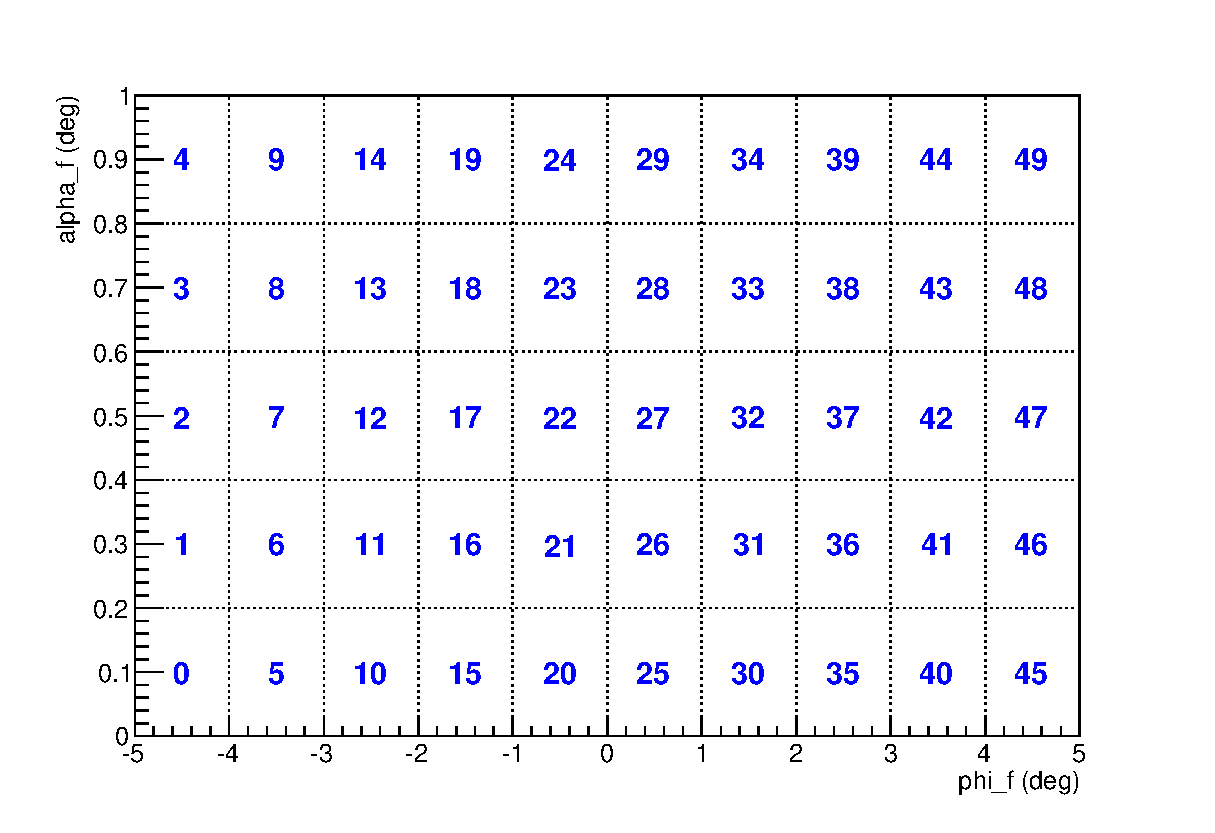
\includegraphics[clip=, width=120mm]{fig/drawing/UserAPI_IntensityDataLayout.eps}
  \caption{The axes layout of IntensityData object.}
  \label{fig:UserApi:IntensityData}
\end{figure}

The x-axis and y-axis of the figure correspond to the $\phi_f$ and $\alpha_f$ axes of the detector.
The x-axis is divided into 10 bins,
with low edge of the first bin set to $-5.0\,{\rm deg}$ and upper edge of the last bin set to $+5.0\,{\rm deg}$.
The y-axis is divided into 5 bins,
with low edge of the first bin set to $0.0\,{\rm deg}$ and upper edge of the last bin set to $1.0\,{\rm deg}$.
There are 50 bins in total (they are marked on the plot with indexes from 0 to 49), each bin will contain one intensity value.

During a standard simulation (i.e. no Monte-Carlo integration involved) intensities are calculated for $\phi_f, \alpha_f$ values corresponding to the bin centers, e.g. the intensity stored in bin\#42 will correspond to $\phi_f=3.5\,{\rm deg}, \alpha_f=0.5\,{\rm deg}$.
\vspace*{2mm}


\Note{
The \Code{IntensityData} object is not intended for direct usage from Python API. The idea is
that the API provides the user with the possibility to export the data from BornAgain internal format to the format of his choice as well as import user's data into BornAgain.
For the moment this functionality is limited to a few options explained below.
We encourage users feedback to implement the support of most requested formats.}


\subsubsection{Import/export of intensity data}
For the moment we provide following options:
\begin{itemize}
\item Import/export of \Code{IntensityData} object from/to \Code{numpy} array.
\item Import/export of \Code{IntensityData} object from/to text file.

\end{itemize}

\paragraph{Export to numpy array}

To export intensity data into  \Code{numpy} array the method \Code{getArray()} should be used
on \Code{IntensityData} object as shown in line \ref{py:UserApi:getArray} of
following code snippet.

\begin{lstlisting}[language=python, style=eclipseboxed]
intensity = simulation.getIntensityData()
array = intensity.getArray() @\label{py:UserApi:getArray}@
...
pylab.imshow(numpy.rot90(array, 1)) @\label{py:UserApi:imshow}@
pylab.show()
\end{lstlisting}

For the detector settings defined in the previous paragraph the dimensions of the resulting array will be (10,5). By using \Code{numpy} indexes the user can get access to the intensity values, e.g.
\Code{array[0][0]} corresponds to the intensity in bin\#0 of \cref{fig:UserApi:IntensityData},
\Code{array[0][4]} to bin\#4,
\Code{array[1][0]} to bin\#5,
\Code{array[8][2]} to bin\#42,
\Code{array[9][4]} to bin\#49.


To plot this resulting numpy array with \Code{matplotlib} it has to be rotated counter-clockwise
to match \Code{matplotlib} conventions as shown in line~\ref{py:UserApi:imshow}.


%\subsubsection{Direct access to the data}
%User can access to the

%\begin{lstlisting}[language=python, style=eclipseboxed]
%for i in range(0, intensity.getAllocatedSize()):
%    print intensity[i]
%\end{lstlisting}


\subsubsection{Importing from numpy array}

To use fitting the user has to load experimental data into BornAgain fitting kernel.
To read experimental data the user has to create
IntensityData object, fill it with the experimental  intensity values and pass
this object to the fitting kernel.

First, the user creates empty \Code{IntensityData} as shown
in line~\ref{py:UserApi:IntensityData} of the following code snippet.
\begin{lstlisting}[language=python, style=eclipseboxed]
data = IntensityData() @\label{py:UserApi:IntensityData}@
data.addAxis(FixedBinAxis("phi_f", 10, -5.0*degree, 5.0*degree)) @\label{py:UserApi:phi_f}@
data.addAxis(FixedBinAxis("alpha_f", 5, 0.0*degree, 1.0*degree)) @\label{py:UserApi:alpha_f}@
...
array = numpy.zeros((10, 5)) # fill array with experimental intensities @\label{py:UserApi:create_array}@
...
data.setRawDataVector(array.flatten().tolist()) @\label{py:UserApi:set_raw}@

fitSuite = FitSuite() @\label{py:UserApi:fit_suite}@
fitSuite.addSimulationAndRealData(simulation, data) @\label{py:UserApi:add_real_data}@
\end{lstlisting}

In lines~\ref{py:UserApi:phi_f}, \ref{py:UserApi:alpha_f} two axes with fixed bin sizes
are defined to represent the detector layout as shown in \cref{fig:UserApi:IntensityData}.
The constructor of \Code{FixedBinAxis} object has the following signature

\begin{lstlisting}[language=python, style=eclipse,numbers=none]
FixedBinAxis(title, nbins, min_angle, max_angle)
\end{lstlisting}

The created \Code{IntensityData} object has to be filled with experimental intensities
using \Code{numpy} array prepared by the user (lines ~\ref{py:UserApi:create_array}-~\ref{py:UserApi:set_raw}). In lines \ref{py:UserApi:fit_suite},\ref{py:UserApi:add_real_data} the fitting kernel is created and initialized with \Code{Simulation} object and
\Code{IntensityData} object representing the experimental data.


\subsubsection{Saving intensity data to text file.}

The special class \Code{IntensityDataIOFactory} is intended for saving the intensity data
in different datafile formats. For the moment, it only supports saving the data in specific BornAgain's text files (the file extention \Code{*.int}).

\begin{lstlisting}[language=python, style=eclipseboxed]
intensity = simulation.getIntensityData()
IntensityDataIOFactory.writeIntensityData(intensity, 'file_name.int')
\end{lstlisting}

\subsubsection{Reading intensity data from a text file.}
The same class is also intended for reading intensity data
from files with different formats. For the moment, it only supports reading the data from text files of special BornAgain's format (the file extention \Code{*.int}).

\begin{lstlisting}[language=python, style=eclipseboxed]
intensity = IntensityDataIOFactory.readIntensityData('file_name.int')
\end{lstlisting}


%%%%%%%%%%%%%%%%%%%%%%%%%%%%%%%%%%%%%%%%%%%%%%%%%%%%%%%%%%%%%%%%%%%%%%%%%%%%%%%%%
%%
%%   BornAgain User Manual
%%
%%   homepage:   http://www.bornagainproject.org
%%
%%   copyright:  Forschungszentrum Jülich GmbH 2015
%%
%%   license:    Creative Commons CC-BY-SA
%%
%%   authors:    Scientific Computing Group at MLZ Garching
%%               C. Durniak, M. Ganeva, G. Pospelov, W. Van Herck, J. Wuttke
%%
%%%%%%%%%%%%%%%%%%%%%%%%%%%%%%%%%%%%%%%%%%%%%%%%%%%%%%%%%%%%%%%%%%%%%%%%%%%%%%%%

\chapter{Particle form factors}\label{SPFF}

\iffalse
%%%%%%%%%%%%%%%%%%%%%%%%%%%%%%%%%%%%%%%%%%%%%%%%%%%%%%%%%%%%%%%%%%%%%%%%%%%%%%%%
\section{Usage}\label{SintroPFF}
%%%%%%%%%%%%%%%%%%%%%%%%%%%%%%%%%%%%%%%%%%%%%%%%%%%%%%%%%%%%%%%%%%%%%%%%%%%%%%%%

\index{Form factor!tutorial}%
\index{Form factor!examples}%
\index{Form factor!custom implementation}%
The online tutorial contains an entire section on
  \tuto{47}{embedded particles}, including several usage examples
  and a \tutoNomar{72}{list of all available form factors}.
  If a particle shape is missing, try to implement a \tutoNomar{107}{custom form factor},
  or/and contact us.

The particles can be rotated in a different direction by using one of
the following transformations: \Code{CreateRotateX($\theta$),
  CreateRotateY($\theta$), CreateRotateZ($\theta$)}, where capital X, Y, Z mark rotations
around the associated axis and $\theta$ is the
angle of rotation from this axis. For example, the following \Code{Python}\ script shows how to rotate a pyramid by $45^{\circ}$ around
the $z$-axis:\\

\setPy
\begin{lstlisting}
    pyramid_ff = ba.FormFactorPyramid(10*nm, 5*nm, 54.73*deg )
    pyramid = ba.Particle(m_particle, pyramid_ff)
    transform = ba.Transform3D.createRotateZ(45*deg)
    particle_layout = ba.ParticleLayout().addParticle(pyramid, transform)
\end{lstlisting}

Particle rotation is demonstrated in the example~\tuto{61}{rotated pyramids}.

For particles that are made of different materials,
the definition % TODO RESTORE ~\cref{EFFdef}
of the form factor~$F(\q)$
must be generalized in obvious ways.
In practice, the most important case is the \E{core-shell particle}.
\index{Inhomogeneous particles}%
\index{Core-shell particles}%
\index{Particle!Core-shell}%
This is supported in \BornAgain\ through the function
\index{ParticleCoreShell@\Code{ParticleCoreShell}}
\setCpp
\begin{lstlisting}
    ParticleCoreShell(const Particle& shell, const Particle& core,
            kvector_t relative_core_position={0., 0., 0.});
\end{lstlisting}
where \Code{shell\_particle} is assumed to be inscribed
in \Code{core\_particle}.
\Code{rel\_\discretionary{}{}{}position}
specifies the position of the
center of the base of the core particle relative
to center of the base of the shell particle.

See the online tutorial for an example with \tuto{59}{core-shell nanoparticles}.

%===============================================================================
\index{Polydispersity!embedded particles}%
\index{Particle!polydispersity}%
\index{Distribution!of particle parameters}%
\index{Form factor!parameter distributions}%
Embedded particles may be \E{polydisperse}, i.~e.\ have statistical distributions
for some or all their numeric parameters.
This is supported in \BornAgain\ through the same mechanism
as for other numeric parameters.

See the online tutorial for the example \tuto{66}{cylinders with size distribution}.
  The example also shows how two parameters can be tied to each other
(size distribution with constant ratio radius/height).

\fi

%%%%%%%%%%%%%%%%%%%%%%%%%%%%%%%%%%%%%%%%%%%%%%%%%%%%%%%%%%%%%%%%%%%%%%%%%%%%%%%%
\section{Hard particles}\label{SHPFF}
%%%%%%%%%%%%%%%%%%%%%%%%%%%%%%%%%%%%%%%%%%%%%%%%%%%%%%%%%%%%%%%%%%%%%%%%%%%%%%%%

\index{Form factor!hard particles|(}

% Don't number subfigures in this chapter.
\makeatletter
\renewcommand{\@thesubfigure}{\relax}
\makeatother

% \lstset{language=python,style=eclipseboxed,numbers=none,nolol}

\def\ffsection#1{%
%\FloatBarrier\clearpage\ifodd\value{page}\E{Page intentionally left blank}\clearpage\else\fi
\subsection{#1}}


\BornAgain\ comes with a comprehensive collection of hard-coded
shape transforms for standard particle geometries like
spheres, cylinders, prisms, pyramids or ripples.
This collection is documented in the following.
For each shape,
the real-space geometry is shown in orthogonal projections,
the parameters of the \BornAgain\ method are defined,
an analytical expression for the form factor is given,
and exemplary results for $\left|F(\q)\right|^2$ versus
$\alpha_\sf,\phi_\sf$ are shown for small-angle scattering conditions
($\alpha_\si=\phi_\si=0$).

The computation of $F(\q)$ is based on
shapes $S(\r)$ given in Cartesian coordinates,
as defined in the orthogonal projections.
Typically, the vertical ($z$) direction is chosen
along a symmetry axis of the particle.
The origin is always at the center of the bottom side of the particle.
Different parametrization or a different choice of the origin
cause our analytic form factors to trivially deviate
from expressions given in the \IsGISAXS\ manual \cite[Sec.~2.3]{Laz08}
or in the literature \cite[Appendix]{ReLL09}.

We recomputed all expressions to make sure
that they also hold for complex scattering vectors,
used to describe in order to take any material absorption into account.
The implementation in \BornAgain\ allows all three components
of~$\q$ to be complex.\footnote
{Per~\cref{Ekconst},
only the vertical components of $\k_\si$ and $\k_\sf$ can have imaginary parts.
However,
for tilted particles
$F(\v{\tilde{q}})$ needs to be computed with
a rotated scattering vector~$\v{\tilde q}$
that may be complex in all three components.}

The following tables summarize the implemented particle geometries,
 roughly ordered by decreasing symmetry.
Afterwards, the detailed documentation is in alphabetical order.

%\clearpage\thispagestyle{empty}
\def\entry#1#2#3#4#5#6{%
\raisebox{-3.8ex}{\includefinal{5em}{fig/blue/#2.png}} &
 \texttt{#1}& %\newline\textsl{#1} &
#5 & % symmetry
#4 & % parameters
Page~\pageref{S#3}\\} % , \cref{S#3}
\begin{center}
  \def\h{\text{h}}
  \def\v{\text{v}}
\small
\begin{longtable}
  {@{}p{.14\textwidth}
   @{}p{.32\textwidth}
   @{}p{.17\textwidth}
   @{}p{.19\textwidth}
   @{}p{.15\textwidth}@{}}
% Shape&{Name\newline \textsl{Legacy Name}}&Symmetry&Parameters&Reference\\\hline
Shape&Name&Symmetry&Parameters&Reference\\\hline
\entry{FullSphere}{FullSphere3d}{FullSphere}{$R$}{R$_3$}{Sphere}
\entry{FullSpheroid}{FullSpheroid3d}{FullSpheroid}{$R$, $H$}{D$_{\infty\h}$}{Spheroid}
\entry{Cylinder}{Cylinder3d}{Cylinder}{$R$, $H$}{D$_{\infty\h}$}{Cylinder}
\entry{TruncatedSphere}{Sphere3d}{TruncatedSphere}{$R$, $H$}{C$_{\infty\v}$}{SphericalCap}
\entry{TruncatedSpheroid}{Spheroid3d}{TruncatedSpheroid}{$R$, $H$, $f_p$}{C$_{\infty\v}$}{SpheroidalCap}
\entry{Cone}{Cone3d}{Cone}{$R$, $H$, $\alpha$}{C$_{\infty\v}$}{ConicalFrustum}
\entry{Icosahedron}{Icosahedron3d}{Icosahedron}{$L$}{I$_\h$}{Icosahedron}
\entry{Dodecahedron}{Dodecahedron3d}{Dodecahedron}{$L$}{I$_\h$}{Dodecahedron}
\entry{TruncatedCube}{TruncatedCube3d}{TruncatedCube}{$L$, $t$}{O$_\h$}{TruncatedCube}
\entry{Prism6}{Prism63d}{Prism6}{$R$, $H$}{D$_{6\h}$}{Prism6}
\entry{Cone6}{Cone63d}{Cone6}{$R$, $H$, $\alpha$}{C$_{6\v}$}{Frustum6}
\entry{Pyramid}{Pyramid3d}{Pyramid}{$L$, $H$, $\alpha$}{C$_{4\v}$}{Frustum4}
\entry{Cuboctahedron}{Cuboctahedron3d}{Cuboctahedron}{$L$, $H$, $r_H$, $\alpha$}{C$_{4\v}$}{BiFrustum4}
\entry{Prism3}{Prism33d}{Prism3}{$L$, $H$}{D$_{3\h}$}{Prism3}
\entry{Tetrahedron}{Tetrahedron3d}{Tetrahedron}{$L$, $H$, $\alpha$}{C$_{3\v}$}{Frustum3}
\entry{EllipsoidalCylinder}{EllipsoidalCylinder3d}{EllipsoidalCylinder}{$R_a$, $R_b$, $H$}{D$_{2\h}$}{EllipsoidalCylinder}
\entry{Box}{Box3d}{Box}{$L$, $W$, $H$}{D$_{2\h}$}{Prism2}
\entry{HemiEllipsoid}{HemiEllipsoid3d}{HemiEllipsoid}{$R_a$, $R_b$, $H$}{C$_{2\v}$}{HemiEllipsoid}
\entry{AnisoPyramid}{AnistropicPyramid3d}{AnisoPyramid}{$L$, $W$, $H$, $\alpha$}{C$_{2\v}$}{Frustum2}
\hline
\end{longtable}
\end{center}
%\thispagestyle{empty}\clearpage

\index{Rotation of particles}
\index{Orientation of particles}
\index{CreateRotateX@\Code{CreateRotateX}}
\index{Transform3D@\Code{Transform3D}}

In the following subsections,
information about the implemented geometries is given in standardized form.
Analytical expressions are given for the form factor $F(\q)$,
for the volume $V=F(0)$,
and for the maximum horizontal section $S$
(the area of the particle as seen from above).
\nomenclature[2s130 0]{$S$}{Maximum horizontal section of embedded particle}%
Mathematical notation in the form factor expressions includes
the cardinal sine functions $\sinc(z)\coloneqq\sin(z)/z$
and the Bessel function of first kind and first order $J_1(z)$
\cite[Ch.~9]{AbSt64}.
\nomenclature[2j132 01]{$J_1$}{Bessel function of first kind and first order}%
If results contain an integral,
then no analytical form was found,
and the integral is evaluated by numeric quadrature.
\index{Quadrature}%
For polyhedral figures,
\index{Polyhedron!form factor}
\index{Form factor!polyhedron}
except a few simple ones like the rectangular box,
we use a generic form factor computation,
parametrized by the vertices of the figure,
that is described in full detail in a mathematical paper~\cite{ba:ffp}.

Almost all analytical expressions for $F(\q)$ contain
removable singularities for certain values of $\q$.
Our implementation uses proper analytic continuations at these singularities,
\index{Form factor!singularities}
\index{Singularitiy!in form factor computation}
though this is not explicitly denoted in the following formula collection.
Furthermore, series expansions are used to ensure numeric accuracies
in the neighborhood of the singularities.
For polyhedra, see Ref.~\cite{ba:ffp} for a meticulous discussion.

\begin{figure}[t]
\begin{center}
\includefinal{1\TW}{fig/ff2/ff_demo_1quadrants.pdf}
\end{center}
\caption{Normalized intensity $I(\alpha_\sf,\phi_\sf)$
for small-angle scattering by a truncated sphere with $R=4.2$~nm and $H=6.1$~nm,
for four different tilt angles~$\vartheta$ (rotation around the $y$ axis).
Since $I$ possess the standard symmetry (\protect\ref{EFq4sym}),
data are only shown for first quadrant $0^\circ\le\phi_\sf,\alpha_\sf\le 5^\circ$.}
\label{F1quadrants}
\end{figure}

Geometrical objects can be parametrized in different ways.
Concerns about user experience and about code readability
sometimes lead to different choices.
For the \BornAgain\ user interfaces (GUI and API)
we have chosen the most standard parameters,
as used in elementary geometry, like length, height, radius,
even if this is at variance from the \IsGISAXS\ precedent.
Where our parametrization made analytic expressions too tedious,
we use alternate internal parameters to alleviate the formul\ae.

Examplary form factors are numerically computed in Born approximation.
The particles are assigned a refractive index of $n=10^{-5}$.
Parameters are chosen such that
the particle volume~$V$ is about 250~nm$^3$ (within $\pm5$~\%);
except ripples, which are chosen with a vertical section $V/L$ of 40~nm$^2$
and a length of 25~nm.
The incident wavelength is 1~\AA.
The incident beam is always in $x$ direction, hence $\alpha_\si=\phi_\si=0$.
Simulated detector images are normalized to the maximum scattering intensity at $F(0)=V$,
\begin{equation}
  I(\alpha_\sf,\phi_\sf)\coloneqq |F(q(\alpha_\sf,\phi_\sf))|^2/V^2.
\end{equation}
All plots have the same logarithmic color scale,
extending over ten decades from $10^{-1)}$ to~1.
Plot ranges in $\alpha_\sf$ and $\phi_\sf$ are also standardized as far as
reasonably possible.
For most particle geometries,
$I$ has horizontal and vertical mirror planes:
\begin{equation}\label{EFq4sym}
  I(\alpha_\sf,\phi_\sf)
  = I(\alpha_\sf,-\phi_\sf)
  = I(-\alpha_\sf,-\phi_\sf)
  = I(\alpha_\sf,-\phi_\sf).
\end{equation}
% TODO RESTORE TEMPORARILY REMOVED XREF
% The physical origin this symmetry is discussed in \cref{Ssym}.
For these particles,
plots of $I$ are restricted to the quadrant $\alpha_\sf\ge0$, $\phi_\sf\ge0$.
However, it requires some experience to fully appreciate the
information content of these plots.
For a demonstration of this,
try to grasp the main features of \cref{F1quadrants}.
Then compare with \cref{F4quadrants}.

\begin{figure}[t]
\begin{center}
\includefinal{1\TW}{fig/ff2/ff_demo_4quadrants.pdf}
\end{center}
\caption{Same data as in Fig.~\protect\ref{F1quadrants},
but now shown for all four quadrants ($-5^\circ\le\phi_\sf,\alpha_\sf\le 5^\circ$).
The vertical interference pattern,
which gradually disappears with increasing tilt angle,
 is much more salient in this plot
than in the preceding one-quadrant representation.}
\label{F4quadrants}
\end{figure}

\index{Large particles!numeric difficulty}%
\index{Numeric difficulty!form factor oscillations}%
\index{Oscillations!from large particle form factor}%
\index{Monte-Carlo integration!for large particle form factor}%
\index{Particle!rapid form factor oscillations}%
\index{Form factor!rapid oscillations}%
\index{Form factor!large particles}%
\Warn{For large particles (typically of order 1000nm),
  the form factor oscillates rapidly within one detector bin
  so that analytical calculations (performed for the bin center)
  may give a completely wrong intensity pattern.}

In this case, the best solution we can currently provide
  is a Monte-Carlo integration, as shown in the example
  \tuto{TODO}{large particle form factor}.

\index{Shape transform!catalogue|(}
\index{Form factor!catalogue|(}

%===============================================================================
\ffsection{AnisoPyramid (rectangle-based)} \label{SAnisoPyramid}
%===============================================================================
  \index{Anisotropic pyramid (form factor)}
  \index{Pyramid (form factor)!rectangular (AnisoPyramid)}
  \index{Truncated pyramid (form factor)!rectangular (AnisoPyramid)}
  \index{FormFactorAnisoPyramid@\Code{FormFactorAnisoPyramid}}

\paragraph{Real-space geometry}\strut\\

\begin{figure}[H]
\hfill
\subfigure[Perspective]{\includefinal{.24\TW}{fig/blue/AnistropicPyramid3d.png}}
\hfill
\subfigure[Top view]{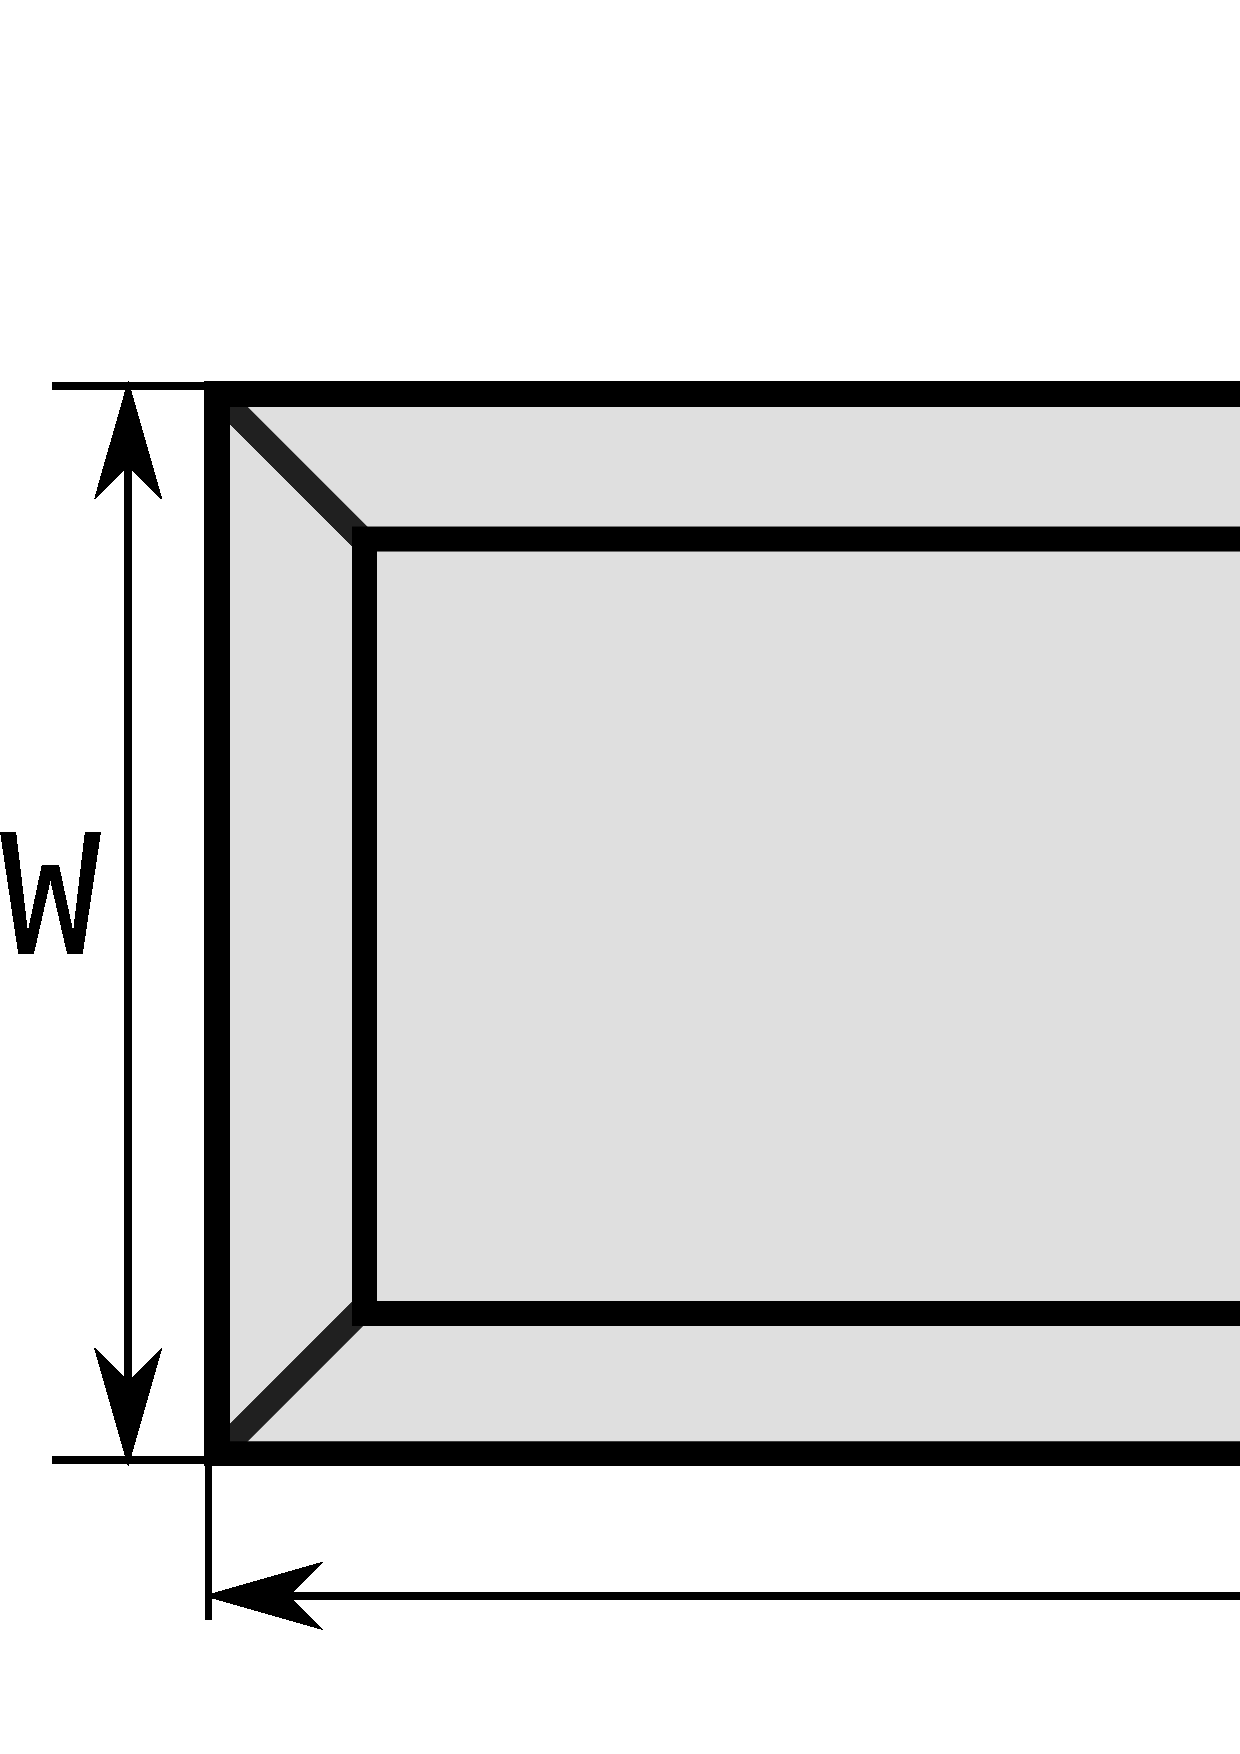
\includegraphics[width=.30\textwidth]{fig/cuts/AnisoPyramid2dxy.pdf}}
\hfill
\subfigure[Side view]{\raisebox{2mm}{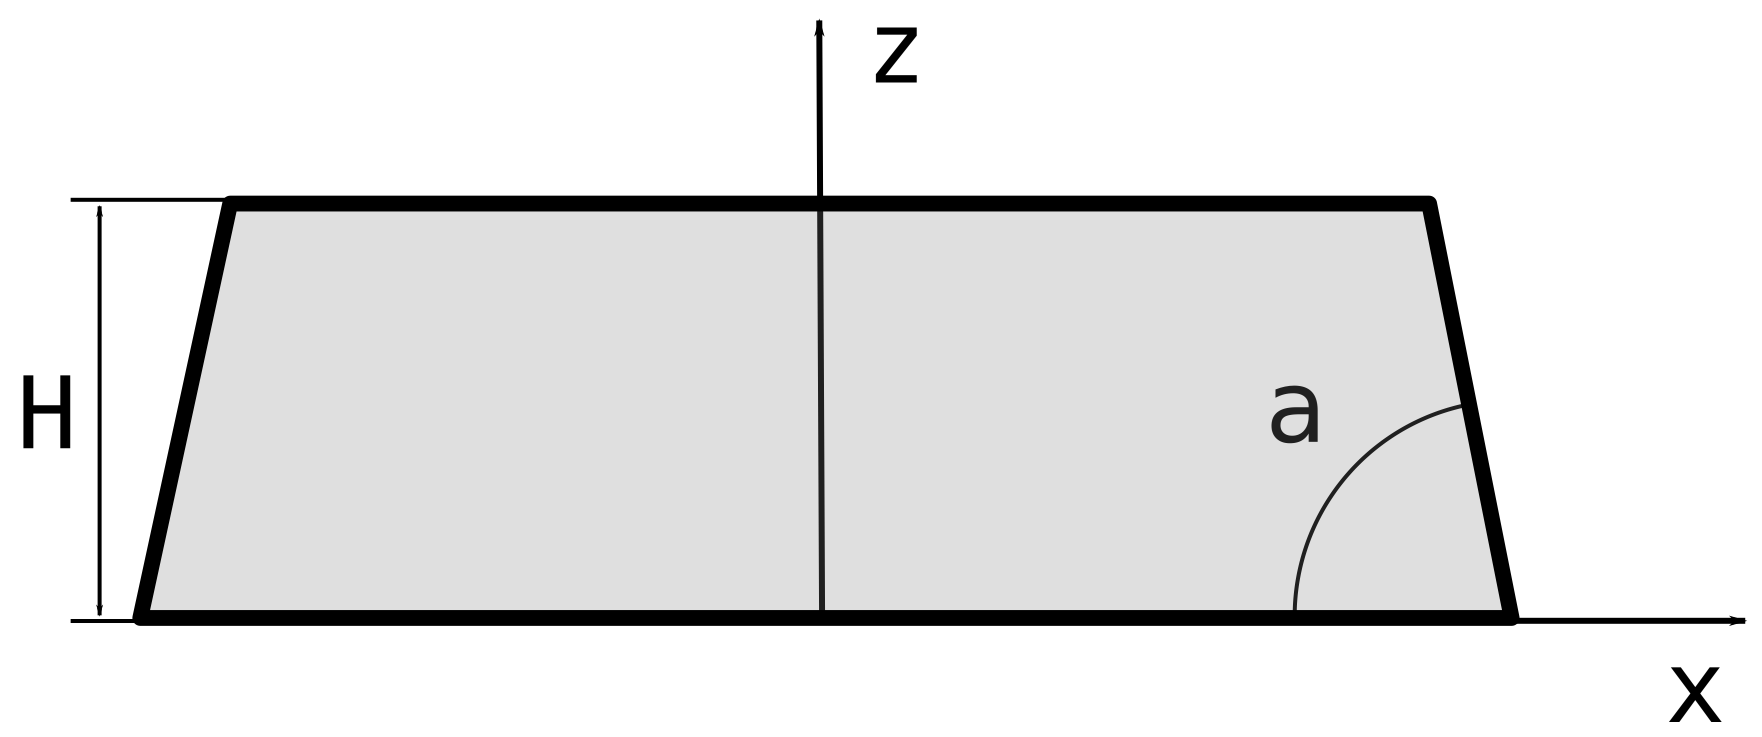
\includegraphics[width=.30\textwidth]{fig/cuts/AnisoPyramid2dxz.pdf}}}
\hfill
\caption{A truncated pyramid with a rectangular base.}
\end{figure}

\FloatBarrier

\paragraph{Syntax and parameters}\strut\\[-2ex plus .2ex minus .2ex]
\begin{lstlisting}
  FormFactorAnisoPyramid(double length, double width, double height, double alpha)
\end{lstlisting}
with the parameters
\begin{itemize}
\item \texttt{length} of the base, $L$,
\item \texttt{width} of the base, $W$,
\item \texttt{height}, $H$
\item \texttt{alpha}, angle between the base and a side face, $\alpha$.
\end{itemize}
They must fulfill
\begin{displaymath}
  H \le \frac{\tan\alpha}{2} \min\,(L,W).
\end{displaymath}

\paragraph{Form factor, volume, horizontal section}\strut\\
\begin{equation*}
  F \text{~: computed using the generic polyhedron form factor~\cite{ba:ffp},}
\end{equation*}
\begin{equation*}
  V= H \Big[LW - \dfrac{(L + W)H}{\tan\alpha} + \dfrac{4}{3} \dfrac{H^2}{\tan^2\alpha}\Big].
\end{equation*}
\begin{equation*}
  S=LW.
\end{equation*}

\paragraph{Examples}\strut\\
\begin{figure}[H]
\begin{center}
\includefinal{1\TW}{fig/ff2/ff_AnisoPyramid.pdf}
\end{center}
\caption{Normalized intensity $|F|^2/V^2$,
computed with $L=13$~nm, $W=8$~nm, $H=4.2$~nm, and $\alpha=60^\circ$,
for four different angles~$\omega$ of rotation around the $z$ axis.}
\label{fig:FFAnisoPyramidEx}
\end{figure}

\paragraph{History}\strut\\
Agrees with the \E{In-plane anisotropic pyramid} form factor of \IsGISAXS\
\cite[Eq.~2.40]{Laz08} \cite[Eq.~217]{ReLL09},
except for different parametrization.
This is \E{not} the \E{anisotropic pyramid} of \FitGISAXS,
which is a true pyramid with an off-center apex \cite{Bab13}.

Formfactors~$F(\q)$ have been checked against the different computation of \IsGISAXS,
and were found to fully agree.

%===============================================================================
\ffsection{Box (cuboid)} \label{SBox}
%===============================================================================
  \index{Box (form factor)}
  \index{Cuboid (form factor)}
  \index{Prism (form factor)!reactangular (Box)}
  \index{Platonic solids!cube}
  \index{FormFactorBox@\Code{FormFactorBox}}

\paragraph{Real-space geometry}\strut\\

\begin{figure}[H]
\hfill
\subfigure[Perspective]{\includefinal{.24\TW}{fig/blue/Box3d.png}}
\hfill
\subfigure[Top view]{\includefinal{.3\TW}{fig/cuts/Box2dxy.pdf}}
\hfill
\subfigure[Side view]{\raisebox{2mm}{\includefinal{.3\TW}{fig/cuts/Box2dxz.pdf}}}
\hfill
\caption{A rectangular cuboid.}
\end{figure}

\FloatBarrier

\paragraph{Syntax and parameters}\strut\\[-2ex plus .2ex minus .2ex]
\begin{lstlisting}
  FormFactorBox(double length, double width, double height)
\end{lstlisting}
with the parameters
\begin{itemize}
\item \texttt{length} of the base, $L$,
\item \texttt{width} of the base, $W$,
\item \texttt{height}, $H$.
\end{itemize}

\paragraph{Form factor, volume, horizontal section}

\begin{equation*}
F= L W H\exp\left(i q_z \frac{H}{2}\right) \sinc\left(q_x \frac{L}{2}\right)
\sinc\left(q_y \frac{W}{2}\right) \sinc\left(q_z \frac{H}{2}\right),
\end{equation*}
\begin{equation*}
  V= LWH,
\end{equation*}
\begin{equation*}
  S = LW.
\end{equation*}

\paragraph{Examples}\strut

\begin{figure}[H]
\begin{center}
\includefinal{1\TW}{fig/ff2/ff_Box.pdf}
\end{center}
\caption{Normalized intensity $|F|^2/V^2$,
computed with $L=18$~nm, $W=4.6$~nm, and $H=3$~nm,
for four different angles~$\omega$ of rotation around the $z$ axis.}
\end{figure}

\paragraph{History}\strut\\
Agrees with \E{Box} form factor of \IsGISAXS\
\cite[Eq.~2.38]{Laz08} \cite[Eq.~214]{ReLL09},
except for factors $1/2$ in the definitions of parameters $L$, $W$, $H$.


%===============================================================================
\ffsection{Cone (circular)} \label{SCone}
%===============================================================================
  \index{Cone (form factor)!circular}
  \index{Truncated cone (form factor)}
  \index{FormFactorCone@\Code{FormFactorCone}}

\paragraph{Real-space geometry}\strut\\

\begin{figure}[H]
\hfill
\subfigure[Perspective]{\includefinal{.24\TW}{fig/blue/Cone3d.png}}
\hfill
\subfigure[Top view]{\includefinal{.3\TW}{fig/cuts/Cone2dxy.pdf}}
\hfill
\subfigure[Side view]{\raisebox{3mm}{\includefinal{.3\TW}{fig/cuts/Cone2dxz.pdf}}}
\hfill
\caption{A truncated cone with circular base.}
\end{figure}

\paragraph{Syntax and parameters}\strut\\[-2ex plus .2ex minus .2ex]
\begin{lstlisting}
  FormFactorCone(double radius, double height, double alpha)
\end{lstlisting}
with the parameters
\begin{itemize}
\item \texttt{radius}, $R$,
\item \texttt{height}, $H$,
\item \texttt{alpha}, angle between the side and the base, $\alpha$.
\end{itemize}
They must fulfill
\begin{displaymath}
  H\le R\tan\alpha.
\end{displaymath}

\paragraph{Form factor, volume, horizontal section}\strut\\
Notation:
\begin{equation*}
  R_H \coloneqq R-\dfrac{H}{\tan \alpha}, \quad
  q_{\parallel} \coloneqq \sqrt{q_x^2+ q_y^2}, \quad
  \tilde{q}_z \coloneqq q_z \tan\alpha.
\end{equation*}
Results:
\begin{equation*}
  F = 2\pi \tan\alpha\; \e^{i\tilde{q}_z R}
      \int_{R_H}^R \!\d\rho\, \rho^2
        \frac{J_1(q_{\parallel}\rho)}{q_{\parallel}\rho}\,\e^{-i\tilde{q}_z \rho},
\end{equation*}
\begin{equation*}
  V = \dfrac{\pi}{3}\tan\alpha  \left( R^3 - R_H^3\right),
\end{equation*}
\begin{equation*}
  S=\pi R^2.
\end{equation*}

\paragraph{Examples}\strut

\begin{figure}[H]
\begin{center}
\includefinal{1\TW}{fig/ff2/ff_Cone.pdf}
\end{center}
\caption{Normalized intensity $|F|^2/V^2$,
computed with $R=4$~nm, $H=11$~nm, and $\alpha=75^\circ$,
for four different tilt angles~$\vartheta$ (rotation around the $y$ axis).}
\end{figure}

\paragraph{History}\strut\\
Agrees with \E{Cone} form factor of \IsGISAXS\
\cite[Eq.~2.28]{Laz08} \cite[Eq.~225]{ReLL09},
except for a substitution $z\to\rho$ in our expression for~$F$.


%===============================================================================
\ffsection{Cone6 (hexagonal)} \label{SCone6}
%===============================================================================
  \index{Cone (form factor)!hexagonal (Cone6)}
  \index{Pyramid (form factor)!hexagonal (Cone6)}
  \index{Truncated pyramid (form factor)!hexagonal (Cone6)}
  \index{FormFactorCone6@\Code{FormFactorCone6}}

\paragraph{Real-space geometry}\strut\\

\begin{figure}[H]
\hfill
\subfigure[Perspective]{\includefinal{.24\TW}{fig/blue/Cone63d.png}}
\hfill
\subfigure[Top view]{\includefinal{.3\TW}{fig/cuts/Cone62dxy.pdf}}
\hfill
\subfigure[Side view]{\raisebox{5mm}{\includefinal{.3\TW}{fig/cuts/Cone62dxz.pdf}}}
\hfill
\caption{A truncated pyramid, based on a regular hexagon}
\end{figure}

\FloatBarrier
\paragraph{Syntax and parameters}\strut\\[-2ex plus .2ex minus .2ex]
\begin{lstlisting}
  FormFactorCone6(double base_edge, double height, double alpha)
\end{lstlisting}
with the parameters
\begin{itemize}
\item \texttt{base\_edge}, edge of the regular hexagonal base, $R$,
\item \texttt{height}, $H$,
\item \texttt{alpha}, dihedral angle between the base and a side face, $\alpha$.
\end{itemize}
Note that the orthographic projection does not show~$\alpha$,
but the angle~$\beta$ between the base and a side edge.
They are related through $\sqrt{3}\tan \alpha = 2 \tan \beta$.
The following is written more conveniently in terms of~$\beta$.
The parameters must fulfill
\begin{displaymath}
  H \le (\tan\beta)R.
\end{displaymath}

\paragraph{Form factor, volume, horizontal section}\strut\\
\begin{equation*}
  F \text{~: computed using the generic polyhedron form factor~\cite{ba:ffp},}
\end{equation*}
\begin{equation*}
  V = \tan\beta  \left( R^3- \left(R-\frac{H}{\tan\beta}\right)^3 \right),
\end{equation*}
\begin{equation*}
  S =\dfrac{3\sqrt{3}R^2}{2}.
\end{equation*}

\paragraph{Examples}\strut

\begin{figure}[H]
\begin{center}
\includefinal{1\TW}{fig/ff2/ff_Cone6.pdf}
\end{center}
\caption{Normalized intensity $|F|^2/V^2$,
computed with $R=6$~nm, $H=5$~nm, and $\alpha=60^\circ$,
for four different angles~$\omega$ of rotation around the $z$ axis.}
\end{figure}

\paragraph{History}\strut\\
Our parametrization deviates from the form factor \E{Cone6} of \IsGISAXS
\cite[Eq.~2.32]{Laz08} \cite[Eq.~222]{ReLL09}.

Up to \BornAgain-1.5 computed by numeric integration, as in \IsGISAXS.
Since \BornAgain-1.6 higher speed and better accuracy are achieved
by using the generic polyhedron form factor \cite{ba:ffp},
with series expansions near singularities.

%===============================================================================
\ffsection{Cuboctahedron} \label{SCuboctahedron}
%===============================================================================
  \index{Cuboctahedron (form factor)}
  \index{Platonic solids!octahedron}
  \index{FormFactorCuboctahedron@\Code{FormFactorCuboctahedron}}

\paragraph{Real-space geometry}\strut\\

\begin{figure}[H]
\hfill
\subfigure[Perspective]{\includefinal{.24\TW}{fig/blue/Cuboctahedron3d.png}}
\hfill
\subfigure[Top view]{\includefinal{.3\TW}{fig/cuts/Cuboctahedron2dxy.pdf}}
\hfill
\subfigure[Side view]{\raisebox{2mm}{\includefinal{.3\TW}{fig/cuts/Cuboctahedron2dxz.pdf}}}
\hfill
\caption{A compound of two truncated pyramids with a common square base
and opposite orientations.}
\end{figure}

\FloatBarrier

\paragraph{Syntax and parameters}\strut\\[-2ex plus .2ex minus .2ex]
\begin{lstlisting}
  FormFactorCuboctahedron(double length, double height, double height_ratio, double alpha)
\end{lstlisting}
with the parameters
\begin{itemize}
\item \texttt{length} of the shared square base, $L$,
\item \texttt{height} of the bottom pyramid, $H$,
\item \texttt{height\_ratio} between the top and the bottom pyramid, $r_H$,
\item \texttt{alpha}, angle between the base and a side face, $\alpha$.
\end{itemize}
They must fulfill
\begin{displaymath}
  H \le \frac{\tan\alpha}{2} L
  \quad\text{and}\quad
  r_h H \le \frac{\tan\alpha}{2} L.
\end{displaymath}

\paragraph{Form factor, volume, horizontal section}\strut\\
\begin{equation*}
  F \text{~: computed using the generic polyhedron form factor~\cite{ba:ffp},}
\end{equation*}
\begin{equation*}
  V= \dfrac{1}{6} \tan(\alpha)L^3 \Big[ 2
         - \Big(1 - \dfrac{2H }{L\tan(\alpha)} \Big)^3
           - \Big(1 - \dfrac{2 r_H
             H}{L\tan(\alpha) }\Big)^3\Big],
\end{equation*}
\begin{equation*}
  S =L^2.
\end{equation*}

\paragraph{Examples}\strut

\begin{figure}[H]
\begin{center}
\includefinal{1\TW}{fig/ff2/ff_Cuboctahedron.pdf}
\end{center}
\caption{Normalized intensity $|F|^2/V^2$,
computed with $L=8$~nm, $H=5$~nm, $r_H=0.5$, and $\alpha=60^\circ$,
for four different angles~$\omega$ of rotation around the $z$ axis.}
\end{figure}

\paragraph{History}\strut\\
Agrees with \E{Cuboctahedron} form factor of \IsGISAXS\
\cite[Eq.~2.34]{Laz08} \cite[Eq.~218]{ReLL09},
except for different parametrization $L=2R_{\rm{\Code{IsGISAXS}}}$.
Since \BornAgain-1.6 implemented
using the generic polyhedron form factor \cite{ba:ffp}.


%===============================================================================
\ffsection{Cylinder} \label{SCylinder}
%===============================================================================
  \index{Cylinder (form factor)}
  \index{FormFactorCylinder@\Code{FormFactorCylinder}}

\paragraph{Real-space geometry}\strut\\

\begin{figure}[H]
\hfill
\subfigure[Perspective]{\includefinal{.24\TW}{fig/blue/Cylinder3d.png}}
\hfill
\subfigure[Top view]{\includefinal{.3\TW}{fig/cuts/Cylinder2dxy.pdf}}
\hfill
\subfigure[Side view]{\raisebox{-2.5mm}{\includefinal{.3\TW}{fig/cuts/Cylinder2dxz.pdf}}}
\hfill
\caption{An upright circular cylinder.}
\end{figure}

\paragraph{Syntax and parameters}\strut\\[-2ex plus .2ex minus .2ex]
\begin{lstlisting}
  FormFactorCylinder(double radius, double height)
\end{lstlisting}
with the parameters
\begin{itemize}
\item \texttt{radius} of the circular base, $R$,
\item \texttt{height}, $H$.
\end{itemize}

\paragraph{Form factor, volume, horizontal section}\strut\\
Notation:
\begin{equation*}
  q_{\parallel} \coloneqq \sqrt{q_x^2+q_y^2}.
\end{equation*}
Note that this does \E{not} involve the sesquilinear product
$|q_x|^2=q_x^* q_x$ but the plain product $q_xq_x$ of complex numbers
(and analogous for~$q_y$).

Results:
\begin{equation*}
  F=  2\pi R^2 H  \sinc\left(q_ z \frac{H}{2}\right) \exp\left(i q_ z \frac{H}{2}\right)
    \frac{J_1(q_{\parallel} R )}{q_{\parallel} R },
\end{equation*}
\begin{equation*}
  V = \pi R^2 H,
\end{equation*}
\begin{equation*}
  S=\pi R^2.
\end{equation*}

\paragraph{Examples}\strut

\begin{figure}[H]
\begin{center}
\includefinal{1\TW}{fig/ff2/ff_Cylinder.pdf}
\end{center}
\caption{Normalized intensity $|F|^2/V^2$,
computed with $R=3$~nm and $H=8.8$~nm,
for four different tilt angles~$\vartheta$ (rotation around the $y$ axis).}
\end{figure}

\paragraph{History and Derivation}\strut\\
For real wave vectors, this form factor is well known;
it goes back to Lord Rayleigh.
In \IsGISAXS, it has been implemented as form factor \E{Cylinder}
\cite[Eq.~2.27]{Laz08} \cite[Eq.~223]{ReLL09},
allowing for complex wavevectors.

Since it is not obvious that the standard formula also holds for complex~$\q$,
let us provide a derivation. We only consider the integral over the polar angle,
\begin{equation}
  I(\q) \coloneqq \int_0^{2\pi}\!\d\varphi\,\exp\left(iq_xr\sin\varphi+iq_yr\cos\varphi\right).
\end{equation}
With the abbreviations $a\coloneqq r(q_x+iq_y)/2$ and $b\coloneqq r(q_x-iq_y)/2$,
\begin{equation}
  I(\q) = \int_0^{2\pi}\!\d\varphi\,\exp\left(a\e^{i\varphi}-b\e^{-i\varphi}\right).
\end{equation}
Expansion of the exponential, combined with a binomial expansion of its argument, yields
\begin{equation}
  I(\q)
  = \int_0^{2\pi}\!\d\varphi\,
  \sum_{n=0}^\infty\sum_{k=0}^n(-)^k\frac{a^{n-k}b^{k}}{(n-k)!k!}\e^{i(n-2k)\varphi}.
\end{equation}
The integral over $\varphi$ vanishes except for $n=2k$. Hence
\begin{equation}
  I(\q)
  = 2\pi \sum_{k=0}^\infty(-)^k\frac{{\sqrt{ab}\,}^{2k}}{k!k!}
  = 2\pi J_0\left(rq_\parallel\right).
\end{equation}
Integration over~$r$ then yields the in-plane contribution to the form factor~$F(\q)$.


%===============================================================================
\ffsection{Dodecahedron} \label{SDodecahedron}
%===============================================================================
  \index{Dodecahedron (form factor)}
  \index{Platonic solids!dodecahedron}
  \index{FormFactorDodecahedron@\Code{FormFactorDodecahedron}}

\paragraph{Real-space geometry}\strut\\

\begin{figure}[H]
\strut\hfill
%\subfigure[Perspective]
{\includefinal{.24\TW}{fig/blue/Dodecahedron3d.png}}
%\hfill
%\subfigure[Top view]{\includefinal{.3\TW}{fig/cuts/Box2dxy.pdf}}
%\hfill
%\subfigure[Side view]{\raisebox{2mm}{\includefinal{.3\TW}{fig/cuts/Box2dxz.pdf}}}
\hfill\strut
\caption{A regular dodecahedron.}
\end{figure}

\FloatBarrier

\paragraph{Syntax and parameters}\strut\\[-2ex plus .2ex minus .2ex]
\begin{lstlisting}
  FormFactorDodecahedron(double edge)
\end{lstlisting}
with the parameter
\begin{itemize}
\item \texttt{edge}, length of one edge, $a$.
\end{itemize}

\paragraph{Form factor, volume, horizontal section}\strut\\
\begin{equation*}
  F \text{~: computed using the generic form factor of a polyhedron
             with inversion symmetry~\cite{ba:ffp},}
\end{equation*}
\begin{equation*}
  V= \frac{1}{4} (15+7\sqrt{5}) a^3 \approx 7.663\,a^3,
\end{equation*}
%\begin{equation*}
%  S = %% wait for Holden, Shapes, Space, and Symmetry
%\end{equation*}

\paragraph{Examples}\strut

\begin{figure}[H]
\begin{center}
\includefinal{1\TW}{fig/ff2/ff_Dodecahedron_sym.pdf}
\end{center}
\caption{Normalized intensity $|F|^2/V^2$,
computed with $a=3.2$~nm,
for three orientations of high symmetry:
$x$ axis perpendicular to a polygonal face;
vertex on the $x$ axis;
edge in the $xy$ plane and perpendicular to the $x$ axis.}
\end{figure}

\begin{figure}[H]
\begin{center}
\includefinal{1\TW}{fig/ff2/ff_Dodecahedron_asy.pdf}
\end{center}
\caption{Normalized intensity $|F|^2/V^2$,
computed with $a=3.2$~nm,
for three orientations of decreasing symmetry:
base pentagon in $xy$ plane and pointing in $x$ direction;
rotated by $13^\circ$ around the $z$ axis;
ditto, and tilted by $9^\circ$ around the $x$ axis.}
\end{figure}

\paragraph{History}\strut\\
New in \BornAgain-1.6,
based on the generic form factor of the polyhedron~\cite{ba:ffp}.


%===============================================================================
\ffsection{EllipsoidalCylinder} \label{SEllipsoidalCylinder}
%===============================================================================
  \index{Ellipsoidal cylinder (form factor)}
  \index{Cylinder (form factor)!ellipsoidal}
  \index{FormFactorEllipsoidalCylinder@\Code{FormFactorEllipsoidalCylinder}}

\paragraph{Real-space geometry}\strut\\

\begin{figure}[H]
\hfill
\subfigure[Perspective]{\includefinal{.24\TW}{fig/blue/EllipsoidalCylinder3d.png}}
\hfill
\subfigure[Top view]{\includefinal{.3\TW}{fig/cuts/EllipsoidalCylinder2dxy.pdf}}
\hfill
\subfigure[Side view]{\raisebox{4mm}{\includefinal{.3\TW}{fig/cuts/EllipsoidalCylinder2dxz.pdf}}}
\hfill
\caption{A upright cylinder whose cross section is an ellipse.}
\end{figure}

\paragraph{Syntax and parameters}\strut\\[-2ex plus .2ex minus .2ex]
\begin{lstlisting}
  FormFactorEllipsoidalCylinder(double radius_a, double radius_b, double height)
\end{lstlisting}
with the parameters
\begin{itemize}
\item \texttt{radius\_a}, in $x$ direction, $R_a$,
\item \texttt{radius\_b}, in $y$ direction, $R_b$,
\item \texttt{height}, $H$.
\end{itemize}

\paragraph{Form factor, volume, horizontal section}\strut\\
Notation:
\begin{equation*}
  \gamma \coloneqq \sqrt{(q_x R_a)^2+(q_y R_b)^2}
\end{equation*}
Results:
\begin{equation*}
F = 2\pi R_a R_b H \exp\left(i\frac{q_z H}{2}\right)
   \sinc\left(\frac{q_z H}{2}\right) \frac{J_1(\gamma)}{\gamma},
\end{equation*}
\begin{equation*}
  V = \pi R_a R_bH,
\end{equation*}
\begin{equation*}
  S = R_a R_b.
\end{equation*}

\paragraph{Examples}\strut

\begin{figure}[H]
\begin{center}
\includefinal{1\TW}{fig/ff2/ff_EllipsoidalCylinder.pdf}
\end{center}
\caption{Normalized intensity $|F|^2/V^2$,
computed with $R_a=6.3$~nm, $R_b=4.2$~nm and $H=3$~nm,
for four different angles~$\omega$ of rotation around the $z$ axis.}
\end{figure}

\paragraph{History}\strut\\
Agrees with the \IsGISAXS\ form factor
\E{Ellipsoid} \cite[Eq.~2.41, wrongly labeled in Fig.~2.4]{Laz08}
or \E{Ellipsoidal Cylinder} \cite[Eq.~224]{ReLL09}.


%===============================================================================
\ffsection{FullSphere} \label{SFullSphere}
%===============================================================================
  \index{Full sphere (form factor)}
  \index{Sphere (form factor)}
  \index{FormFactorFullSphere@\Code{FormFactorFullSphere}}

\paragraph{Real-space geometry}\strut\\

\begin{figure}[H]
\hfill
\subfigure[Perspective]{\includefinal{.24\TW}{fig/blue/FullSphere3d.png}}
\hfill
\subfigure[Top view]{\includefinal{.3\TW}{fig/cuts/FullSphere2dxy.pdf}}
\hfill
\subfigure[Side view]{\raisebox{-2mm}{\includefinal{.3\TW}{fig/cuts/FullSphere2dxz.pdf}}}
\hfill
\caption{A full sphere.}
\end{figure}

\FloatBarrier

\paragraph{Syntax and parameters}\strut\\[-2ex plus .2ex minus .2ex]
\begin{lstlisting}
  FormFactorFullSphere(double radius)
\end{lstlisting}
with the parameter
\begin{itemize}
\item \texttt{radius}, $R$.
\end{itemize}

\paragraph{Form factor, volume, horizontal section}\strut\\
Notation:
\begin{equation*}
  q \coloneqq \sqrt{q_x^2+q_y^2+q_z^2}.
\end{equation*}
Note that this does \E{not} involve the sesquilinear product
$|q_x|^2=q_x^* q_x$ but the plain product $q_xq_x$ of complex numbers
(and analogous for~$q_y$, $q_z$).
\begin{equation*}
F = \frac{4\pi}{q^3} \exp(iq_z R)\left[\sin(qR) - qR \cos(qR)\right],
\end{equation*}
\begin{equation*}
  V = \dfrac{4\pi}{3}R^3,
\end{equation*}
\begin{equation*}
  S= \pi R^2.
\end{equation*}

\paragraph{Example}\nopagebreak\strut\nopagebreak

\begin{figure}[H]
\begin{center}
\includefinal{.5\TW}{fig/ff2/ff_FullSphere.pdf}
\end{center}
\caption{Normalized intensity $|F|^2/V^2$,
computed with $R=3.9$~nm.}
\end{figure}

\paragraph{History and Derivation}\strut\\
For real wave vectors, this form factor is well known;
it goes back at least to Lord Rayleigh.
In \IsGISAXS, it has been implemented as form factor \E{Full sphere}
\cite[Eq.~2.36]{Laz08} \cite[Eq.~226]{ReLL09},
allowing for complex wavevectors.
Since it is not obvious that Rayleigh's formula also holds for complex~$\q$,
let us outline a derivation
(if you know a more elegant one, we would like to hear).

If the origin is at the center of the sphere, then the form factor is
\begin{equation}
I(\q,R)
 = \int_0^R\d r\, r^2\int_0^{\pi}\d\theta\,\sin\theta\int_0^{2\pi}\d\varphi
  \:\e^{i\q\r}
\end{equation}
with $\q\r
= q_x r\sin\theta\cos\varphi + q_y r\sin\theta\sin\varphi + q_z r\cos\theta$.
For the integration over $\varphi$,
see \cref{SCylinder} on the form factor of a cylinder:
\begin{equation}
  I(\q,R)
  = 2\pi \int_0^R \d r\,r^2 \int_0^{\pi} \d\theta\, \sin\theta
   \exp\left(i q_z \cos \theta\right) J_0\left(q_\parallel r\sin \theta\right)
\end{equation}
with $q_{\parallel}=\sqrt{q_x^2+q_y^2}$.
By symmetry, the imaginary part is zero,
so that the exponential reduces to a cosine:
\begin{equation}
  I(\q,R)
  = 2\pi \int_0^R \d r\,r^2 \int_0^{\pi} \d\theta\, \sin\theta
   \cos\left(q_z \cos \theta\right) J_0\left(q_\parallel r\sin \theta\right).
\end{equation}
Expand the cosine and the Bessel function:
\begin{equation}
  I(\q,R)
  = 2\pi \int_0^R \d r\,r^2 \int_0^{\pi} \d\theta\, \sin\theta
    \sum_{j=0}^\infty (-)^j \frac{(q_zr\cos\theta)^{2j}}{(2j)!}\,
    \sum_{k=0}^{\infty} (-)^k \frac{(q_\parallel r \sin\theta)^{2k}}{4^k k!^2}.
\end{equation}
Sort by powers of $r$, and integrate:
\begin{equation}
  I(\q,R)
  = 2\pi \sum_{n=0}^\infty (-)^n \frac{R^{2n+3}}{2n+3} \sum_{k=0}^n
    \frac{{q_z}^{2n-2k}}{(2n-2k)!}\,\frac{{q_\parallel}^{2k}}{4^k k!^2} \zeta(k,n)
\end{equation}
with
\begin{equation}
  \zeta(k,n)
  \coloneqq \int_0^{\pi} \d\theta\, \sin\theta
  (\cos\theta)^{2n-2k}(\sin\theta)^{2k}.
\end{equation}
This integral \cite[no.\ 2.512.4]{GrRy07} yields
\begin{equation}
  \zeta(k,n)
  = \frac{2^{2k+1}(2n-2k)! n! k!}{(2n+1)!(n-k)!}.
\end{equation}
Hence
\begin{equation}\label{ESphereU}
  I(\q,R)
  = 4\pi \sum_{n=0}^\infty (-)^n \frac{R^{2n+3}}{(2n+3)(2n+1)!}
    \sum_{k=0}^n \frac{n!}{(n-k)!k!}{q_z}^{2n-2k}{q_\parallel}^{2k}.
\end{equation}
The inner sum happens to be the binomial expansion of
$q^{2n}=\left({q_z}^2+{q_\parallel}^2\right)^n$.
Therefore \cref{ESphereU} coincides with the series expansion of
\begin{equation}
  I(\q,R)
  = 4\pi q^{-3} \left( \sin(qR) - qR\cos(qR) \right),
\end{equation}
which is what we wanted to prove.

%===============================================================================
\ffsection{FullSpheroid} \label{SFullSpheroid}
%===============================================================================
  \index{Full spheroid (form factor)}
  \index{Spheroid (form factor)}
  \index{FormFactorFullSpheroid@\Code{FormFactorFullSpheroid}}

\paragraph{Real-space geometry}\strut\\

\begin{figure}[H]
\hfill
\subfigure[Perspective]{\includefinal{.24\TW}{fig/blue/FullSpheroid3d.png}}
\hfill
\subfigure[Top view]{\includefinal{.3\TW}{fig/cuts/FullSpheroid2dxy.pdf}}
\hfill
\subfigure[Side view]{\raisebox{-3mm}{\includefinal{.3\TW}{fig/cuts/FullSpheroid2dxz.pdf}}}
\hfill
\caption{A full spheroid, generated by rotating an ellipse around the vertical axis.}
\end{figure}

\FloatBarrier

\paragraph{Syntax and parameters}\strut\\[-2ex plus .2ex minus .2ex]
\begin{lstlisting}
  FormFactorFullSpheroid(double radius, double height)
\end{lstlisting}
with the parameters
\begin{itemize}
\item \texttt{radius}, $R$,
\item \texttt{height}, $H$.
\end{itemize}

\paragraph{Form factor, volume, horizontal section}\strut\\
Notation:
\begin{equation*}
 R_z \coloneqq R\sqrt{1-\frac{4z^2}{H^2}},\quad
 q_\plll \coloneqq \sqrt{q_x^2+q_y^2}.
\end{equation*}
Results:
\begin{equation*}
  F = 4\pi \exp(i q_z H/2) \int_0^{H/2} \!\d z\,
     R_z^2 \frac{J_1(q_{\parallel}R_z)}{q_{\parallel}R_z} \cos(q_z z),
\end{equation*}
\begin{equation*}
  V =\dfrac{2}{3}R^2H,
\end{equation*}
\begin{equation*}
  S =\pi R^2.
\end{equation*}

\paragraph{Example}\strut

\begin{figure}[H]
\begin{center}
\includefinal{.5\TW}{fig/ff2/ff_FullSpheroid.pdf}
\end{center}
\caption{Normalized intensity $|F|^2/V^2$,
computed with $R=3.5$~nm and $H=9.8$~nm.}
% changes very little under tilt !
\end{figure}

\paragraph{History}\strut\\
Agrees with the \E{Full spheroid} form factor of \IsGISAXS\
\cite[Eq.~2.37]{Laz08} \cite[Eq.~227]{ReLL09},
with corrected volume formula.
We also discovered a wrong factor of~2 in the \IsGISAXS\ code.


%===============================================================================
\ffsection{HemiEllipsoid} \label{SHemiEllipsoid}
%===============================================================================
  \index{Hemi ellipsoid (form factor)}
  \index{Ellipsoid (form factor)!truncated}
  \index{Truncated ellipsoid (form factor)}
  \index{FormFactorHemiEllipsoid@\Code{FormFactorHemiEllipsoid}}

\paragraph{Real-space geometry}\strut\\

\begin{figure}[H]
\hfill
\subfigure[Perspective]{\includefinal{.24\TW}{fig/blue/HemiEllipsoid3d.png}}
\hfill
\subfigure[Top view]{\includefinal{.3\TW}{fig/cuts/HemiEllipsoid2dxy.pdf}}
\hfill
\subfigure[Side view]{\raisebox{5mm}{\includefinal{.3\TW}{fig/cuts/HemiEllipsoid2dxz.pdf}}}
\hfill
\caption{An horizontally oriented ellipsoid, truncated at the central plane.}
\end{figure}

\paragraph{Syntax and parameters}\strut\\[-2ex plus .2ex minus .2ex]
\begin{lstlisting}
  FormFactorHemiEllipsoid(double radius_a, double radius_b, double height)
\end{lstlisting}
with the parameters
\begin{itemize}
\item \texttt{radius\_a}, in $x$ direction, $R_a$,
\item \texttt{radius\_b}, in $y$ direction, $R_b$,
\item \texttt{height}, equal to radius in $z$ direction, $H$
\end{itemize}

\paragraph{Form factor, volume, horizontal section}\strut\\
Notation:
\begin{equation*}
 r_{a,z} \coloneqq R_a \sqrt{1-\left(\dfrac{z}{H} \right)^2},\quad
 r_{b,z} \coloneqq R_b \sqrt{1-\left(\dfrac{z}{H} \right)^2}, \quad
 \gamma_z =\sqrt{(q_x r_{a,z})^2+(q_y r_{b,z})^2}.
\end{equation*}
Results:
\begin{equation*}
  F = 2\pi \int_0^{H} \!\d z\, r_{a,z} r_{b,z}
                               \frac{J_1(\gamma_z)}{\gamma_z}\exp(iq_z z),
\end{equation*}
\begin{equation*}
  V = \dfrac{2}{3}\pi R_a R_bH,
\end{equation*}
\begin{equation*}
  S =\pi R_a R_b.
\end{equation*}

\paragraph{Examples}\strut

\begin{figure}[H]
\begin{center}
\includefinal{1\TW}{fig/ff2/ff_HemiEllipsoid.pdf}
\end{center}
\caption{Normalized intensity $|F|^2/V^2$,
computed with $R_a=10$~nm, $R_b=3.8$~nm and $H=3.2$~nm,
for four different angles~$\omega$ of rotation around the $z$ axis.}
\end{figure}

\paragraph{History}\strut\\
Agrees with the \IsGISAXS\ form factor
\E{Anisotropic hemi-ellipsoid}
\cite[Eq.~2.42, with wrong sign in the $z$-dependent phase factor]{Laz08}
or \E{Hemi-spheroid} \cite[Eq.~229]{ReLL09}.


%===============================================================================
\ffsection{Icosahedron} \label{SIcosahedron}
%===============================================================================
  \index{Icosahedron (form factor)}
  \index{Platonic solids!icosahedron}
  \index{FormFactorIcosahedron@\Code{FormFactorIcosahedron}}

\paragraph{Real-space geometry}\strut\\

\begin{figure}[H]
\strut\hfill
%\subfigure[Perspective]
{\includefinal{.24\TW}{fig/blue/Icosahedron3d.png}}
%\hfill
%\subfigure[Top view]{\includefinal{.3\TW}{fig/cuts/Box2dxy.pdf}}
%\hfill
%\subfigure[Side view]{\raisebox{2mm}{\includefinal{.3\TW}{fig/cuts/Box2dxz.pdf}}}
\hfill\strut
\caption{A regular icosahedron.}
\end{figure}

\FloatBarrier

\paragraph{Syntax and parameters}\strut\\[-2ex plus .2ex minus .2ex]
\begin{lstlisting}
  FormFactorIcosahedron(double edge)
\end{lstlisting}
with the parameter
\begin{itemize}
\item \texttt{edge}, length of one edge, $a$.
\end{itemize}

\paragraph{Form factor, volume, horizontal section}\strut\\
\begin{equation*}
  F \text{~: computed using the generic form factor of a polyhedron
             with inversion symmetry~\cite{ba:ffp},}
\end{equation*}
\begin{equation*}
  V= \frac{5}{12} (3+\sqrt5)a^3 \approx 2.182\,a^3
\end{equation*}
%\begin{equation*}
%  S = %% wait for Holden, Shapes, Space, and Symmetry
%\end{equation*}

\paragraph{Examples}\strut

\begin{figure}[H]
\begin{center}
\includefinal{1\TW}{fig/ff2/ff_Icosahedron_sym.pdf}
\end{center}
\caption{Normalized intensity $|F|^2/V^2$,
computed with $a=4.8$~nm,
for three orientations of high symmetry:
$x$ axis perpendicular to a polygonal face;
vertex on the $x$ axis;
edge in the $xy$ plane and perpendicular to the $x$ axis.}
\end{figure}

\begin{figure}[H]
\begin{center}
\includefinal{1\TW}{fig/ff2/ff_Icosahedron_asy.pdf}
\end{center}
\caption{Normalized intensity $|F|^2/V^2$,
computed with $a=4.8$~nm,
for three orientations of decreasing symmetry:
base pentagon in $xy$ plane and pointing in $x$ direction;
rotated by $13^\circ$ around the $z$ axis;
ditto, and tilted by $9^\circ$ around the $x$ axis.}
\end{figure}

\paragraph{History}\strut\\
New in \BornAgain-1.6,
based on the generic form factor of the polyhedron~\cite{ba:ffp}.


%===============================================================================
\ffsection{Prism3 (triangular)} \label{SPrism3}
%===============================================================================
  \index{Prism (form factor)!triangular (Prism3)}
  \index{FormFactorPrism3@\Code{FormFactorPrism3}}

\paragraph{Real-space geometry}\strut\\

\begin{figure}[H]
\hfill
\subfigure[Perspective]{\includefinal{.24\TW}{fig/blue/Prism33d.png}}
\hfill
\subfigure[Top view]{\includefinal{.3\TW}{fig/cuts/Prism32dxy.ps}}
\hfill
\subfigure[Side view]{\includefinal{.3\TW}{fig/cuts/Prism32dxz.ps}}
\hfill
\caption{A prism based on an equilateral triangle.}
\end{figure}

\FloatBarrier

\paragraph{Syntax and parameters}\strut\\[-2ex plus .2ex minus .2ex]
\begin{lstlisting}
  FormFactorPrism3(double length, double height)
\end{lstlisting}
with the parameters
\begin{itemize}
\item \texttt{length} of one base edge, $L$,
\item \texttt{height}, $H$.
\end{itemize}

\paragraph{Form factor, volume, horizontal section}\strut\\
\begin{equation*}
F = H \sinc\left(q_z\frac{H}{2}\right) \exp\left(-i q_z\frac{ H}{2}\right) F_\parallel(\q_\parallel)
\end{equation*}
with the form factor $F_\parallel$ of the base triangle
computed using the generic form factor of a planar polygon \cite{ba:ffp},
\begin{equation*}
  V= \dfrac{\sqrt{3}}{4} H L^2,
\end{equation*}
\begin{equation*}
  S =\dfrac{\sqrt{3}}{4}L^2.
\end{equation*}

\paragraph{Examples}\strut

\begin{figure}[H]
\begin{center}
\includefinal{1\TW}{fig/ff2/ff_Prism3.pdf}
\end{center}
\caption{Normalized intensity $|F|^2/V^2$,
computed with $L=13.8$~nm and $H=3$~nm,
for four different angles~$\omega$ of rotation around the $z$ axis.}
\label{fig:FFprism3Ex}
\end{figure}

\paragraph{History}\strut\\
Has been validated against the \E{Prism3} form factor of \IsGISAXS\
\cite[Eq.~2.29]{Laz08} \cite[Eq.~219]{ReLL09}.
Note the different parameterization $L= 2 R_{\rm{\Code{IsGISAXS}}}$.
In \FitGISAXS\ just called \E{Prism} \cite{Bab13}.
In \BornAgain-1.6,
redefined to let the $x$ axis point along a symmetry axis
(rotated by $30^\circ$ with respect to the previous version).

Reimplemented in \BornAgain-1.6 using the generic form factor
of a polygonal prism \cite{ba:ffp},
to achieve numerical stability near the removable singularity at $q\to0$.

%===============================================================================
\ffsection{Prism6 (hexagonal)} \label{SPrism6}
%===============================================================================
  \index{Prism (form factor)!hexagonal (Prism6)}
  \index{FormFactorPrism6@\Code{FormFactorPrism6}}

\paragraph{Real-space geometry}\strut\\

\begin{figure}[H]
\hfill
\subfigure[Perspective]{\includefinal{.24\TW}{fig/blue/Prism63d.png}}
\hfill
\subfigure[Top view]{\includefinal{.3\TW}{fig/cuts/Prism62dxy.pdf}}
\hfill
\subfigure[Side view]{\raisebox{-3mm}{\includefinal{.3\TW}{fig/cuts/Prism62dxz.pdf}}}
\hfill
\caption{A prism based on a regular hexagon.}
\end{figure}

\FloatBarrier

\paragraph{Syntax and parameters}\strut\\[-2ex plus .2ex minus .2ex]
\begin{lstlisting}
  FormFactorPrism6(double radius, double height)
\end{lstlisting}
with the parameters
\begin{itemize}
\item \texttt{radius} of the hexagonal base, $R$,
\item \texttt{height}, $H$.
\end{itemize}

\paragraph{Form factor, volume, horizontal section}\strut\\
\begin{equation*}
F = H \sinc\left(q_z\frac{H}{2}\right) \exp\left(-i q_z\frac{ H}{2}\right) F_\parallel(\q_\parallel)
\end{equation*}
with the form factor $F_\parallel$ of the base hexagon
computed using the generic form factor of a planar polygon
with two-fold symmetry~($S_2$) \cite{ba:ffp},
\begin{equation*}
  V = \dfrac{3\sqrt{3}}{2}H R^2,
\end{equation*}
\begin{equation*}
  S =\dfrac{3\sqrt{3}R^2}{2}.
\end{equation*}

\paragraph{Examples}\strut\nopagebreak

\begin{figure}[H]
\begin{center}
\includefinal{1\TW}{fig/ff2/ff_Prism6.pdf}
\end{center}
\caption{Normalized intensity $|F|^2/V^2$,
computed with $R=5.7$~nm and $H=3$~nm,
for four different angles~$\omega$ of rotation around the $z$ axis.}
\label{fig:FFprism6Ex}
\end{figure}

\paragraph{History}\strut\\
Has been validated against the \E{Prism6} form factor of \IsGISAXS\
\cite[Eq.~2.31]{Laz08} \cite[Eq.~221]{ReLL09},
which has different parametrization
and lacks a factor $H$ in $F(\q)$.

Reimplemented in \BornAgain-1.5 using the generic form factor
of a polygonal prism with symmetry~$S_2$ \cite{ba:ffp},
to achieve numerical stability near the removable singularity at $q\to0$.


%===============================================================================
\ffsection{Pyramid (square-based)}\label{SPyramid}
%===============================================================================
  \index{Pyramid (form factor)!square}
  \index{Truncated pyramid (form factor)!square}
  \index{FormFactorPyramid@\Code{FormFactorPyramid}}

\paragraph{Real-space geometry}\strut\\

\begin{figure}[H]
\hfill
\subfigure[Perspective]{\includefinal{.24\TW}{fig/blue/Pyramid3d.png}}
\hfill
\subfigure[Top view]{\includefinal{.3\TW}{fig/cuts/Pyramid2dxy.pdf}}
\hfill
\subfigure[Side view]{\raisebox{2mm}{\includefinal{.3\TW}{fig/cuts/Pyramid2dxz.pdf}}}
\hfill
\caption{A truncated pyramid with a square base.}
\end{figure}

\FloatBarrier

\paragraph{Syntax and parameters}\strut\\[-2ex plus .2ex minus .2ex]
\begin{lstlisting}
  FormFactorPyramid(double length, double height, double alpha)
\end{lstlisting}
with the parameters
\begin{itemize}
\item \texttt{length} of one edge of the square base, $L$,
\item \texttt{height}, $H$,
\item \texttt{alpha}, angle between the base and a side face, $\alpha$,
\end{itemize}
They must fulfill
\begin{displaymath}
  H \le \frac{\tan\alpha}{2}L.
\end{displaymath}

\paragraph{Form factor, volume, horizontal section}\strut\\
\begin{equation*}
  F \text{~: computed using the generic polyhedron form factor~\cite{ba:ffp},}
\end{equation*}
\begin{equation*}
  V = \dfrac{1}{6}  L^3 \tan\alpha\left[ 1
             - \left(1 - \dfrac{2H}{L\tan\alpha}\right)^3 \right],,
\end{equation*}
\begin{equation*}
  S = L^2.
\end{equation*}

\paragraph{Examples}\strut

\begin{figure}[H]
\begin{center}
\includefinal{1\TW}{fig/ff2/ff_Pyramid.pdf}
\end{center}
\caption{Normalized intensity $|F|^2/V^2$,
computed with $L=10$~nm, $H=4.2$~nm and $\alpha=60^{\circ}$,
for four different angles~$\omega$ of rotation around the $z$ axis.}
\end{figure}

\paragraph{History}\strut\\
Corresponds to \E{Pyramid} form factor of \IsGISAXS\
\cite[Eq.~2.31]{Laz08} \cite[Eq.~221]{ReLL09},
except for different parametrization $L=2R_{\rm{\Code{IsGISXAXS}}}$
and a corrected sign.

Reimplemented in \BornAgain-1.6 using the generic form factor
of a polygonal prism \cite{ba:ffp},
to achieve numerical stability near the removable singularity at $q\to0$.


%===============================================================================
\ffsection{Tetrahedron} \label{STetrahedron}
%===============================================================================
  \index{Tetrahedron (form factor)}
  \index{Truncated tetrahedron (form factor)}
  \index{Platonic solids!tetrahedron}
  \index{FormFactorTetrahedron@\Code{FormFactorTetrahedron}}

\paragraph{Real-space geometry}\strut\\

\noindent
Incorrectly named so, since it actually has five, not four surfaces.

\begin{figure}[H]
\hfill
\subfigure[Perspective]{\includefinal{.24\TW}{fig/blue/Tetrahedron3d.png}}
\hfill
\subfigure[Top view]{\includefinal{.3\TW}{fig/cuts/Tetrahedron2dxy.ps}}
\hfill
\subfigure[Side view]{\includefinal{.3\TW}{fig/cuts/Tetrahedron2dxz.ps}}
\hfill
\caption{A truncated pyramid, based on an equilateral triangle.}
\end{figure}

\FloatBarrier

\paragraph{Syntax and parameters}\strut\\[-2ex plus .2ex minus .2ex]
\begin{lstlisting}
  FormFactorTetrahedron(double length, double height, double alpha)
\end{lstlisting}
with the parameters
\begin{itemize}
\item \texttt{length} of one edge of the equilateral triangular base, $L$,
\item \texttt{height}, $H$,
\item \texttt{alpha}, dihedral angle between the base and a side face, $\alpha$.
\end{itemize}
They must fulfill
\begin{displaymath}
  H\le \frac{\tan{\alpha}}{2\sqrt{3}} L.
\end{displaymath}
The orthographic projection also shows the angle~$\beta$ between the base and a side edge.
It is related to the dihedral angle through $\tan \alpha = 2 \tan \beta$.

\paragraph{Form factor, volume, horizontal section}\strut\\
\begin{equation*}
  F\text{~: computed using the generic polyhedron form factor~\cite{ba:ffp},}
\end{equation*}
\begin{equation*}
  V= \dfrac{\tan(\alpha) L^3}{24} \left[1- \left(1 -
  \dfrac{2\sqrt{3} H}{L \tan(\alpha)} \right)^3\right],
\end{equation*}
\begin{equation*}
  S =\dfrac{\sqrt{3}}{4}L^2.
\end{equation*}

\paragraph{Examples}\strut

\begin{figure}[H]
\begin{center}
\includefinal{1\TW}{fig/ff2/ff_Tetrahedron.pdf}
\end{center}
\caption{Normalized intensity $|F|^2/V^2$,
computed with $L=12$~nm, $H=8$~nm, and $\alpha=75^\circ$,
for four different angles~$\omega$ of rotation around the $z$ axis.
The low symmetry requires other angular ranges than used in most other figures.}
\end{figure}

\paragraph{History}\strut\\
Previous implementations as \E{Tetrahedron} in \IsGISAXS\
\cite[Eq.~2.30]{Laz08} \cite[Eq.~220]{ReLL09},
and as  \E{Truncated tetrahedron} in \FitGISAXS\ \cite{Bab13}.
In \BornAgain-1.6,
redefined to let the $x$ axis lie in a mirror plane
(rotated by $30^\circ$ with respect to the previous version).

Up to \BornAgain-1.5, we computed the form factor by numeric integration, as in \IsGISAXS.
Since \BornAgain-1.6 higher speed and accuracy are achieved
by using the generic polyhedron form factor \cite{ba:ffp},
with series expansions near singularities.

%===============================================================================
\ffsection{TruncatedCube} \label{STruncatedCube}
%===============================================================================
  \index{Cube (form factor)!facetted}
  \index{Facetted cube (form factor)}
  \index{FormFactorTruncatedCube@\Code{FormFactorTruncatedCube}}

\paragraph{Real-space geometry}\strut\\

\begin{figure}[H]
\hfill
\subfigure[Perspective]{\includefinal{.24\TW}{fig/blue/TruncatedCube3d.png}}
\hfill
\subfigure[Top view]{\includefinal{.3\TW}{fig/cuts/Truncatedcube2dxy.pdf}}
\hfill
\subfigure[Side view]{\includefinal{.3\TW}{fig/cuts/Truncatedcube2dxz.pdf}}
\hfill
\caption{A cube whose eight vertices have been removed.
The truncated part of each vertex is a trirectangular tetrahedron.}
\end{figure}

\FloatBarrier

\paragraph{Syntax and parameters}\strut\\[-2ex plus .2ex minus .2ex]
\begin{lstlisting}
  FormFactorTruncatedCube(double length, double removed_length)
\end{lstlisting}
with the parameters
\begin{itemize}
\item \texttt{length} of the full cube, $L$,
\item \texttt{removed\_length}, side length of the trirectangular tetrahedron removed from the cube's vertices, $t$.
\end{itemize}
They must fulfill
\begin{displaymath}
  t \le L/2.
\end{displaymath}

\paragraph{Form factor, volume, horizontal section}\strut\\
\begin{equation*}
  F \text{~: computed using the generic form factor of a polyhedron
             with inversion symmetry~\cite{ba:ffp},}
\end{equation*}
\begin{equation*}
  V = L^3 - \dfrac{4}{3}t^3,
\end{equation*}
\begin{equation*}
  S = L^2.
\end{equation*}

\paragraph{Examples}\strut

\begin{figure}[H]
\begin{center}
\includefinal{1\TW}{fig/ff2/ff_TruncatedCube.pdf}
\end{center}
\caption{Normalized intensity $|F|^2/V^2$,
computed with $L=25$~nm, $W=10$~nm, $H=8$~nm, and $d=5$~nm,
for four different angles~$\omega$ of rotation around the $z$ axis.}
\end{figure}

\paragraph{History}\strut\\
Motivated by \cite{HeSS74}.
Reimplemented in \BornAgain-1.6 using the generic form factor
of a polygonal prism \cite{ba:ffp}.


%===============================================================================
\ffsection{TruncatedSphere}\label{STruncatedSphere}
%===============================================================================
  \index{Sphere (form factor)!truncated}
  \index{Truncated sphere (form factor)}
  \index{FormFactorTruncatedSphere@\Code{FormFactorTruncatedSphere}}

\paragraph{Real-space geometry}\strut\\

\begin{figure}[H]
\hfill
\subfigure[Perspective]{\includefinal{.24\TW}{fig/blue/Sphere3d.png}}
\hfill
\subfigure[Top view]{\includefinal{.3\TW}{fig/cuts/Sphere2dxy.pdf}}
\hfill
\subfigure[Side view]{\raisebox{-2mm}{\includefinal{.3\TW}{fig/cuts/Sphere2dxz.pdf}}}
\hfill
\caption{A truncated sphere.}
\end{figure}
\FloatBarrier

\paragraph{Syntax and parameters}\strut\\[-2ex plus .2ex minus .2ex]
\begin{lstlisting}
  FormFactorTruncatedSphere(double radius, double height)
\end{lstlisting}
with the parameters
\begin{itemize}
\item \texttt{radius}, $R$,
\item \texttt{height}, $H$.
\end{itemize}
They must fulfill
\begin{displaymath}
   0 < H\leq 2R.
\end{displaymath}

\paragraph{Form factor, volume, horizontal section}\strut\\
Notation:
\begin{equation*}
  q_{\parallel} \coloneqq \sqrt{q_x^2+q_y^2},\quad
  R_z \coloneqq \sqrt{R^2-z^2}.
\end{equation*}
Results:
\begin{equation*}
F= 2\pi \exp[i q_z (H-R)]\int_{R-H}^{R}\!\d z\, R_z^2
       \frac{J_1(q_{\parallel} R_z) }{q_{\parallel} R_z} \exp(i q_z z) dz,
\end{equation*}
\begin{equation*}
  V=\pi R^3 \left[\dfrac{2}{3} + \dfrac{H-R}{R} - \dfrac{1}{3}\left(\dfrac{H-R}{R}\right)^3\right],
\end{equation*}
\begin{equation*}
  S = \left\{\begin{array}{ll} \pi R^2, & H \geq R \\
         \pi\left(2RH-H^2\right), & H < R \end{array}\right..
\end{equation*}

\paragraph{Example}\strut

\begin{figure}[H]
\begin{center}
\includefinal{1\TW}{fig/ff2/ff_TruncatedSphere.pdf}
\end{center}
\caption{Normalized intensity $|F|^2/V^2$,
computed with $R=4.2$~nm and $H=6.1$~nm,
for four different tilt angles~$\vartheta$ (rotation around the $y$ axis).}
\end{figure}

\paragraph{History}\strut\\
Agrees with the \IsGISAXS\ form factor
\E{Sphere} \cite[Eq.~2.33]{Laz08} or
\E{Truncated sphere} \cite[Eq.~228]{ReLL09}.


%===============================================================================
\ffsection{TruncatedSpheroid} \label{STruncatedSpheroid}
%===============================================================================
  \index{Spheroid (form factor)!truncated}
  \index{Truncated spheroid (form factor)}
  \index{FormFactorTruncatedSpheroid@\Code{FormFactorTruncatedSpheroid}}

\paragraph{Real-space geometry}\strut\\

\begin{figure}[H]
\hfill
\subfigure[Perspective]{\includefinal{.24\TW}{fig/blue/Spheroid3d.png}}
\hfill
\subfigure[Top view]{\raisebox{5mm}{\includefinal{.3\TW}{fig/cuts/Spheroid2dxy.pdf}}}
\hfill
\subfigure[Side view]{\includefinal{.3\TW}{fig/cuts/Spheroid2dxz.pdf}}
\hfill
\caption{A vertically oriented, horizontally truncated spheroid.}
\end{figure}

\paragraph{Syntax and parameters}\strut\\[-2ex plus .2ex minus .2ex]
\begin{lstlisting}
  FormFactorTruncatedSpheroid(double radius, double height, double height_flattening)
\end{lstlisting}
with the parameters
\begin{itemize}
\item \texttt{radius}, $R$,
\item \texttt{height}, $H$.
\item \texttt{height\_flattening}, $f_p$.
\end{itemize}
They must fulfill
\begin{displaymath}
  0< \dfrac{H}{R}\le 2f_p.
\end{displaymath}

\paragraph{Form factor, volume, horizontal section}\strut\\
Notation:
\begin{equation*}
  q_{\parallel} \coloneqq \sqrt{q_x^2+q_y^2}, \quad
  R_z \coloneqq \sqrt{R^2-z^2/f_p^2}.
\end{equation*}
Results:
\begin{equation*}
F =   2\pi \exp[iq_z(H-f_pR)] \int_{f_p R-H}^{f_p R} \!\d z\,
     R_z^2\frac{J_1(q_{\parallel}R_z)}{q_{\parallel}R_z} \exp(i q_z z)
\end{equation*}
\begin{equation*}
  V = \dfrac{\pi R H^2}{f_p}  \Big(1-\dfrac{H}{3f_p R}\Big),
\end{equation*}
\begin{equation*}
  S = \left\{\begin{array}{ll} \pi R^2, & H \geq f_pR \\
         \pi\left(\dfrac{2RH}{f_p}-\dfrac{H^2}{f_p^2}\right), & H < R \end{array}\right..
\end{equation*}

\paragraph{Example}\strut

\begin{figure}[H]
\begin{center}
\includefinal{1\TW}{fig/ff2/ff_TruncatedSpheroid.pdf}
\end{center}
\caption{Normalized intensity $|F|^2/V^2$,
computed with $R=3.3$~nm, $H=9.8$~nm, and $f_p=1.8$,
for four different tilt angles~$\vartheta$ (rotation around the $y$ axis).}
\end{figure}

\paragraph{History}\strut\\
Agrees with the \IsGISAXS\ form factor
\E{Sphere} \cite[Eq.~2.33]{Laz08} or
\E{TruncatedSpheroid} \cite[Eq.~228]{ReLL09}.
% Note an erroneous factor~2 in the expression of the volume
% in the \Code{IsGISAXS} manual.

\index{Shape transform!catalogue|)}
\index{Form factor!catalogue|)}

%%%%%%%%%%%%%%%%%%%%%%%%%%%%%%%%%%%%%%%%%%%%%%%%%%%%%%%%%%%%%%%%%%%%%%%%%%%%%%%%
\section{Ripples}\label{SRipple}
%%%%%%%%%%%%%%%%%%%%%%%%%%%%%%%%%%%%%%%%%%%%%%%%%%%%%%%%%%%%%%%%%%%%%%%%%%%%%%%%


%===============================================================================
\ffsection{Ripple1 (sinusoidal)} \label{SRipple1}
%===============================================================================
  \index{Ripple (form factor)!sinusoidal (Ripple1)}
  \index{Sinusoidal ripple (form factor)}
  \index{FormFactorRipple1@\Code{FormFactorRipple1}}

\paragraph{Real-space geometry}\strut\\

\begin{figure}[H]
\hfill
\subfigure[Perspective]{\includefinal{.24\TW}{fig/blue/Ripple13d.png}}
\hfill
\subfigure[Top view]{\includefinal{.3\TW}{fig/cuts/Ripple12dxy.pdf}}
\hfill
\subfigure[Side view]{\includefinal{.3\TW}{fig/cuts/Ripple12dyz.pdf}}
\hfill
\caption{A ripple with a sinusoidal profile.}
\end{figure}

\paragraph{Syntax and parameters}\strut\\[-2ex plus .2ex minus .2ex]
\begin{lstlisting}
  FormFactorRipple1(double length, double width, double height)
\end{lstlisting}
with the parameters
\begin{itemize}
\item \texttt{length}, $L$,
\item \texttt{width}, $W$,
\item \texttt{height}, $H$.
\end{itemize}

The ripple is modelled as a surface
\begin{equation*}
  Z(y) = \frac{H}{2}\left[ 1 + \cos\frac{2\pi y}{W} \right].
\end{equation*}

\paragraph{Form factor}\strut\\
Using the inverse profile
\begin{equation*}
  Y(z) = \frac{W}{2\pi}\text{arccos}\left( \frac{2z}{H}-1 \right),
\end{equation*}
the form factor is computed by numeric integration:
\begin{equation*}
F = L \sinc\left(\frac{q_xL}{2}\right)
   \int_0^H\!\d z\,\e^{iq_zz}\, 2Y(z)\sinc\left(q_y Y(z)\right).
\end{equation*}
The integration is substantially accelerated by the substitution
$u=\text{arccos}( 2z/H-1)$.

\paragraph{Volume, horizontal section}\strut\\
\begin{equation*}
  V = \dfrac{L W H}{2},
\end{equation*}
\begin{equation*}
  S = L W.
\end{equation*}

\paragraph{Examples}\strut

\begin{figure}[H]
\begin{center}
\includefinal{1\TW}{fig/ff2/ff_Ripple1.pdf}
\end{center}
\caption{Normalized intensity $|F|^2/V^2$,
computed with $L=25$~nm, $W=10$~nm and $H=8$~nm,
for four different angles~$\omega$ of rotation around the $z$ axis.}
\end{figure}

\paragraph{History}\strut\\
Agrees with the \E{Ripple1} form factor of \FitGISAXS\ \cite{Bab13}.

%===============================================================================
\ffsection{Ripple2 (saw-tooth)} \label{SRipple2}
%===============================================================================
  \index{Ripple (form factor)!saw-tooth (Ripple2)}
  \index{Saw-tooth ripple (form factor)}
  \index{FormFactorRipple2@\Code{FormFactorRipple2}}

\paragraph{Real-space geometry}\strut\\

\begin{figure}[H]
\hfill
\subfigure[Perspective]{\includefinal{.24\TW}{fig/blue/Ripple23d.png}}
\hfill
\subfigure[Top view]{\includefinal{.3\TW}{fig/cuts/Ripple22dxy.pdf}}
\hfill
\subfigure[Side view]{\includefinal{.3\TW}{fig/cuts/Ripple22dyz.pdf}}
\hfill
\caption{A ripple with an asymmetric saw-tooth profile.}
\end{figure}

\FloatBarrier

\paragraph{Syntax and parameters}\strut\\[-2ex plus .2ex minus .2ex]
\begin{lstlisting}
  FormFactorRipple2(double length, double width, double height, asymmetry)
\end{lstlisting}
with the parameters
\begin{itemize}
\item \texttt{length}, $L$,
\item \texttt{width}, $W$,
\item \texttt{height}, $H$.
\item \texttt{asymmetry}, $d$.
\end{itemize}
They must fulfill
\begin{displaymath}
  |d| \le W/2.
\end{displaymath}

\paragraph{Form factor, volume, horizontal section}\strut\\
\begin{align*}
F &=L W
\sinc\left(\frac{q_xL}{2}\right)\times \\ &
\int_0^H \!\d z\,
\left(1-\frac{z}{H}\right)
 \sinc\left[\frac{q_y
    W}{2}\left(1-\frac{z}{H}\right)\right]
\exp\left\{ i\left[q_zz -
    q_yd\left(1-\frac{z}{H}\right)\right]\right\}
\end{align*}
\begin{equation*}
  V = \dfrac{L W H}{2},
\end{equation*}
\begin{equation*}
  S = L W.
\end{equation*}

\paragraph{Examples}\strut

\begin{figure}[H]
\begin{center}
\includefinal{1\TW}{fig/ff2/ff_Ripple2.pdf}
\end{center}
\caption{Normalized intensity $|F|^2/V^2$,
computed with $L=25$~nm, $W=10$~nm, $H=8$~nm, and $d=5$~nm,
for four different angles~$\omega$ of rotation around the $z$ axis.
The low symmetry requires other angular ranges than used in most other figures.}
\end{figure}

\paragraph{History}\strut\\
Agrees with the \E{Ripple2} form factor of \FitGISAXS\ \cite{Bab13}.

\index{Form factor!hard particles|)}


\appendix %\addtocontents{toc}{\protect\setcounter{tocdepth}{1}}
%%%%%%%%%%%%%%%%%%%%%%%%%%%%%%%%%%%%%%%%%%%%%%%%%%%%%%%%%%%%%%%%%%%%%%%%%%%%%%%%
%%
%%   BornAgain User Manual
%%
%%   homepage:   http://www.bornagainproject.org
%%
%%   copyright:  Forschungszentrum Jülich GmbH 2015
%%
%%   license:    Creative Commons CC-BY-SA
%%   
%%   authors:    Scientific Computing Group at MLZ Garching
%%               C. Durniak, M. Ganeva, G. Pospelov, W. Van Herck, J. Wuttke
%%
%%%%%%%%%%%%%%%%%%%%%%%%%%%%%%%%%%%%%%%%%%%%%%%%%%%%%%%%%%%%%%%%%%%%%%%%%%%%%%%%

\chapter{Some proofs}  \label{sec:Proofs}

This appendix contains proofs that were taken out of the main text
in order not to disrupt the physics narration.

%%%%%%%%%%%%%%%%%%%%%%%%%%%%%%%%%%%%%%%%%%%%%%%%%%%%%%%%%%%%%%%%%%%%%%%%%%%%%%%%
\section{Source-detector reciprocity for the scalar Schrödinger equation}
  \label{Sreci1}
%%%%%%%%%%%%%%%%%%%%%%%%%%%%%%%%%%%%%%%%%%%%%%%%%%%%%%%%%%%%%%%%%%%%%%%%%%%%%%%%

\textit{reciprocity}
\index{Reciprocity|(}%
\index{Green function!reciprocity}%
of Green functions for self-adjoint differential equations.

Let us derive the reciprocity theorem
for a generic stationary Schrödinger equation
with an isolated inhomogeneity,
\begin{equation}\label{EgsSchrodi}
  \left\{\Nabla^2+v(\r)\right\}G(\r,\rS) = \delta(\r-\rS).
\end{equation}
We assume that $\rS$ lies within our sample.
Outside the sample volume
the potential~$v(\r)$ has the constant value~$K^2$
so that (\ref{EgsSchrodi})
reduces to the Helmholtz equation%
\begin{equation}\label{EgsSchrodiHelmh}
  \left\{\Nabla^2+K^2\right\}G(\r,\rS) = 0.
\end{equation}
We introduce the adjoint Green function~$B$
\nomenclature[2b030 2r040 2r041]{$B(\r,\r')$}{Green function, adjoint of $G$}%
that originates from a source term at the detector location
and obeys
\begin{equation}\label{EgsSchrodiAdj}
  \left\{\Nabla^2+v(\r)\right\}B(\r,\rD) = \delta(\r-\rD).
\end{equation}
We also introduce the auxiliary vector field
\begin{equation}
  \v{X}(\r,\rS,\rD):=B(\r,\rD)\Nabla G(\r,\rS) - G(\r,\rS)\Nabla B(\r,\rD).
\end{equation}
\nomenclature[2x150 2r040]{$\v{X}(\r,\rS,\rD)$}{Auxiliary vector field}%
We inscribe the sample, the detector, and the origin of the coordinate system
into a sphere $\Sphere$ with radius~$R$,
\nomenclature[2s180]{$\Sphere$}{Auxiliary spherical volume}%
\nomenclature[2r120]{$R$}{Radius of $\Sphere$}%
and compute the volume integral
\begin{equation}\label{Eprerecipro}
  \begin{array}{lcl}
    I(\rS,\rD)
  &=& \displaystyle\int_\Sphere\!\d^3r\,\Nabla \v{X}(\r,\rS,\rD)
  \\[1.8em]
  &=& \displaystyle\int_\Sphere\!\d^3r\,\left(
    B\Nabla^2 G- G\Nabla^2 B \right)
  \\[1.4em]
  &=&  B(\rS,\rD) - G(\rD,\rS).
  \end{array}
\end{equation}
Alternatively, we can compute $I$ as a surface integral
\begin{equation}
  I(\rS,\rD)
  =\displaystyle\int_{\partial\Sphere}\d\v{\sigma}\,\v{X}(\r,\rS,\rD)
  =\displaystyle\int_{\partial\Sphere}\d{\sigma}\,
       \left(B\partial_R G - G\partial_R B\right).
\end{equation}
On the surface $\partial\Sphere$,
$B$ and $G$ are outgoing wave fields that obey the Helmholtz equation.
Solutions of this equation in spherical coordinates
have a well-known series expansion.
We send $R\to\infty$ so that we need only to retain the lowest order,
the form of which has been anticipated
in the boundary condition~(\ref{Escabouco}),
\begin{equation}
   G(\r(R,\vartheta,\varphi),\rS)
   \doteq \frac{\e^{iKR}}{4\pi R} g(\vartheta,\varphi),
\end{equation}
and similarly 
\begin{equation}
   B(\r(R,\vartheta,\varphi),\rD)
   \doteq \frac{\e^{iKR}}{4\pi R} b(\vartheta,\varphi).
\end{equation}
The functions $g$ and $b$ can be further expanded into spherical harmonics,
but this is of no interest here.
The decisive point is the factorization of $G$ and $B$
and their common $R$ dependence.
It follows at once that
\begin{equation}
  I(\rS,\rD)
  =\displaystyle\int_{\partial\Sphere}\d\sigma\,
       (\text{$R$-dependent})(bg-gb)
  = 0.
\end{equation}
From (\ref{Eprerecipro}) we obtain the \textit{reciprocity theorem}
\begin{equation}\label{Ereci}
  G(\rD,\rS) = B(\rS,\rD).
\end{equation}
To obtain the forward-propagating Green function~$G$,
it is sufficient to determine the adjoint Green function~$B$
that traces a neutron back from the detector position~$\rD$
to a scattering center~$\rS$.
\index{Reciprocity|)}%

The solution $B(\r,\rD)$ of (\ref{EgsSchrodiAdj})
is analogous to (\ref{EGreens1}).
Choosing the origin inside the sample,
and assuming that $\rD$ lies far outside the sample,
we can copy the far-field expansion from~(\ref{EGreenFar})
to obtain
\index{Far-field approximation}%
\begin{equation}\label{EBFar}
  B_\text{far}(\r,\rD)
  =\frac{\e^{iKr_\text{D}}}{4\pi r_\text{D}}\e^{-i\k_\tf \r}.
\end{equation}
When this backward propagating plane waves impinges on the sample,
it undergoes reflection and refraction in exactly the same way as
the incident plane wave $\e^{i\k_\ti\r}$.
Therefore,
 (\ref{EBFar}) admits a generalization that also holds inside the sample:
\begin{equation}\label{EBFull}
  B_\text{far}(\r,\rD)
  = \frac{\e^{iKr_\text{D}}}{4\pi r_\text{D}}\psi^*_\tf(\r).
\end{equation}
Applying now the reciprocity theorem (\ref{Ereci}),
we can conclude that the far-field Green function
is still given by (\ref{EGreenFar}),
though $\psi_\tf$ no longer is a plane wave.
Accordingly,
the scattered far-field is still given by (\ref{EsandwichC}),
and the differential cross section by (\ref{Exsection}).



\otherchapter{Bibliography}{Bib}
\bibliographystyle{switch}
\bibliography{jw7}

\otherchapter{List of Symbols}{Sym}
\chapter*{List of Symbols}
\label{Snomencl}
\printnomenclature[6em]

\otherchapter{Index}{Idx}
\small
\printindex

\end{document}
